\documentclass[10pt]{book}
\usepackage{../styles/weltbuch}



% Hyperref bitte im main.tex lassen (sollte fast zuletzt geladen werden)
\usepackage{hyperref}
\hypersetup{colorlinks=true, linkcolor=blue, citecolor=teal, urlcolor=magenta}

\begin{document}
	
	% Optional: Titel-/Cover-Seite
	% \begin{titlepage}
		%   \centering
		%   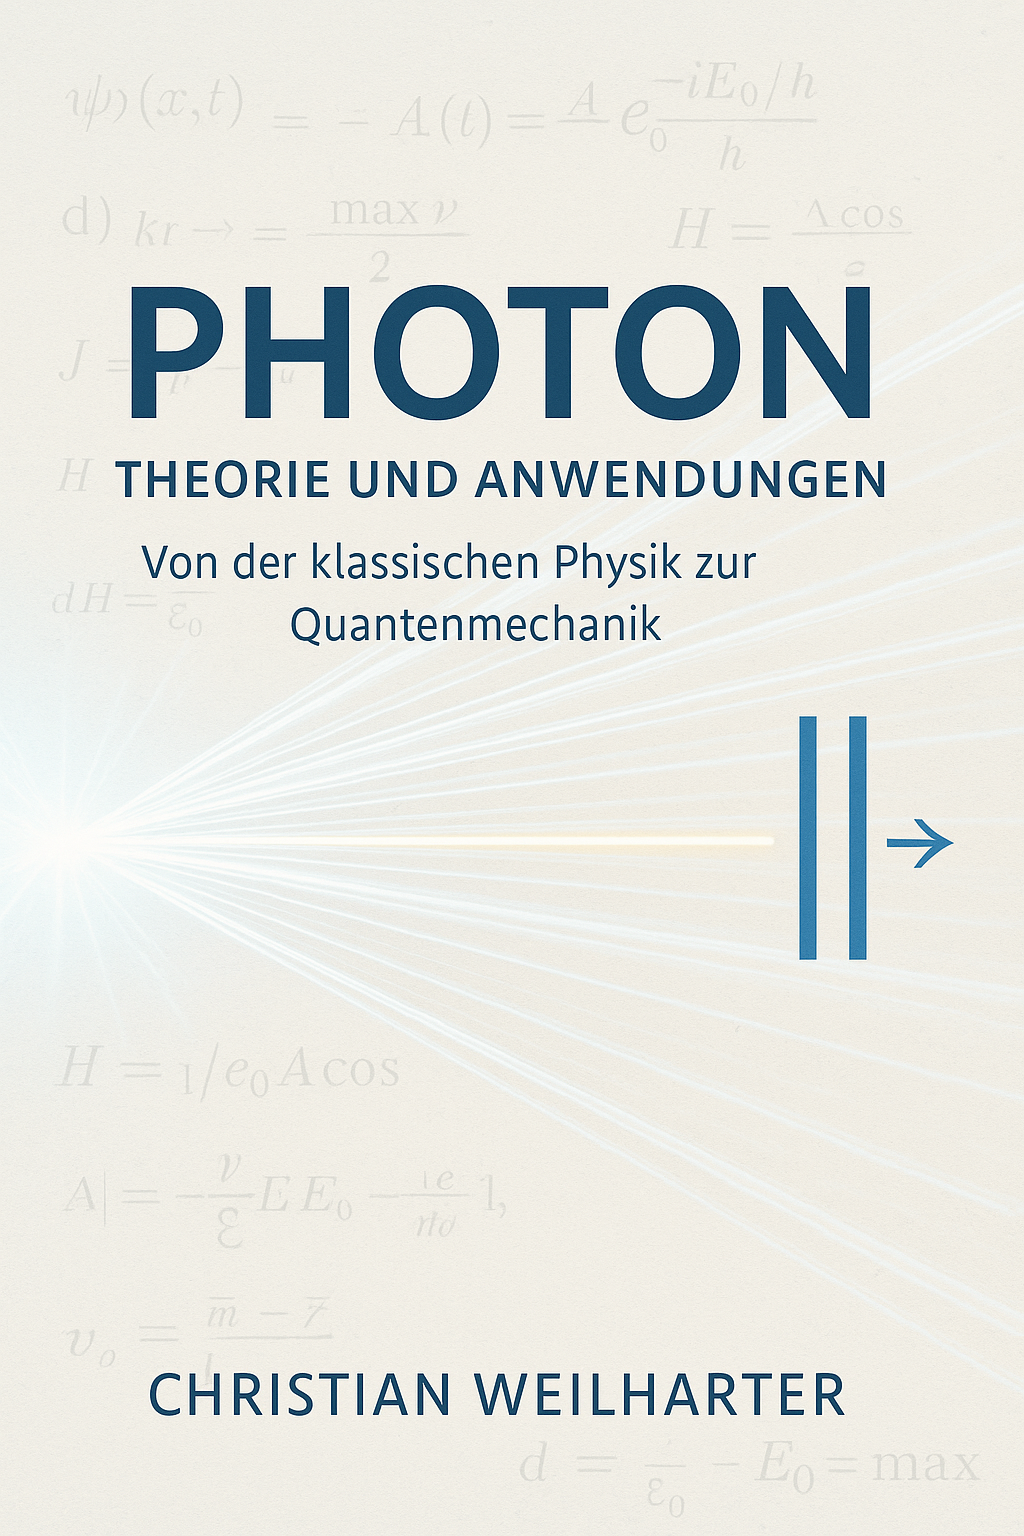
\includegraphics[width=\textwidth]{bilder/cover.png}
		% \end{titlepage}
	
	\hyphenation{exis-tiert}
	
	% Vorwort, ToC
	\cleardoublepage
\thispagestyle{empty}
\begin{center}
	
	{\Large\textbf{Photon – Theory and Applications}}\\[1.2em]
	{\large Dipl.-Ing.\,(FH)\,Christian Weilharter}\\[1.2em]
	\textcopyright~2025, Christian Weilharter, Traunstein\\[2em]
\end{center}

\begin{flushleft}
	\begin{tabular}{@{}l l}
		\textbf{ISBN (Print):} & 978-3-912302-02-8 \\[0.5em]
		\textbf{ISBN (E-Book):} & 978-3-912302-03-5 \\[0.5em]
		\textbf{Edition:} & 1st edition, 2025 \\[0.5em]
		\textbf{Typesetting:} & \LaTeX \\[0.5em]
		\textbf{Publisher:} & Self-published by Christian Weilharter \\[0.5em]

		\textbf{Print:} & Amazon KDP (Print-on-Demand) \\[0.5em]
		\textbf{E-book edition:} & Apple Books \\[0.5em]
		& Amazon Kindle Direct Publishing \\[0.5em]
		\textbf{Contact:} & \href{mailto:info@mathandphysics.de}{info@mathandphysics.eu} \\[0.5em]
		\textbf{Web:} & \href{https://www.mathandphysics.de}{www.mathandphysics.eu} \\

	\end{tabular}
\end{flushleft}

\vspace{2em}
\noindent
All rights reserved. No part of this book may be reproduced, stored, or transmitted
in any form or by any means, electronic or mechanical, including photocopying,
recording, or by any information storage and retrieval system, without prior written
permission of the author.

\begin{center}\small Printed in Germany\end{center}

\cleardoublepage


\chapter*{Preface}
\markboth{Preface}{Preface} % optional für Kopfzeile
% kein addcontentsline → Preface erscheint NICHT im Inhaltsverzeichnis



The creation of this book has been driven by a deep fascination with light and its fundamental mediator – the photon. In modern physics, the photon plays a central role: as a particle without mass, yet carrying energy and momentum; as the messenger of the electromagnetic interaction; and as a key figure in quantum mechanics.  
\noindent
My goal has been to present this multifaceted concept in its historical development, its physical significance, and its technical applications in such a way that both interested laypersons and advanced readers gain a solid understanding – without unnecessary oversimplification, yet always in a clear and accessible manner.  
\noindent
In the conception and preparation of this book, modern technology was also employed. The AI system ChatGPT by OpenAI (as of 2025) was used in a supportive role for formulating, structuring, and reflecting on the content. This collaboration made it possible to articulate ideas more quickly, test alternative phrasings, and clarify complex relationships.  
All content, however, was critically reviewed, revised, and is solely the responsibility of the author.  
\noindent
Thus, this book is not only a contribution to the didactics of modern physics – it is also an experiment in how traditional science can gain a new level of clarity and accessibility through modern tools.  
\noindent
I hope that the enthusiasm for this subject will resonate with the readers – just as it has accompanied me for many years.  

\begin{flushright}
	\textit{Dipl.-Ing.(FH) Christian Weilharter} \\
	\vspace{0.5em}
	[Traunstein, 2025]
\end{flushright}

	\tableofcontents
	
	% Hauptkapitel
	\chapter{Einführung: Theorie und Anwendungen des Photons}\index{Photon}\index{Licht}\index{Quantenmechanik}\index{Quantenfeldtheorie}\index{Quantenelektrodynamik (QED)}

\setcounter{section}{1}
\setcounter{subsection}{0}
\setcounter{subsubsection}{1}
\setcounter{secnumdepth}{3}
\setlength{\parindent}{0pt}
% Boxen-Stile definieren
\tcbset{physikbox/.style={colback=blue!5!white, colframe=blue!75!black, fonttitle=\bfseries}}
\tcbset{mathebox/.style={colback=green!5!white, colframe=green!50!black, fonttitle=\bfseries}}
\tcbset{didaktikbox/.style={colback=yellow!5!white, colframe=yellow!50!black, fonttitle=\bfseries}}
\tcbset{hypobox/.style={colback=orange!5!white, colframe=orange!75!black, fonttitle=\bfseries}}
\tcbset{hinweisbox/.style={colback=gray!10!white, colframe=black!40!black, fonttitle=\bfseries}}

\subsection{Motivation und historische Entwicklung}
\subsubsection{Die zentrale Rolle des Lichts in Naturwissenschaft und Technik}

Licht ist für die Naturwissenschaften weit mehr als ein bloßes Studienobjekt – es ist ein universeller Informationsträger, ein präzises Werkzeug und ein grundlegendes Bindeglied zwischen Theorie und Messung.\index{Informationsträger (Licht)} In gewisser Weise ist Licht das „Auge der Physik“: Ohne Licht würden wir weder in den Kosmos blicken können noch in die inneren Strukturen der Materie.

\subsubsection*{Licht als Erkenntnismittel – Vom Fernrohr zum Teilchenbeschleuniger}
\phantomsection
Die Astronomie wäre ohne Licht schlicht undenkbar.\index{Astronomie} Schon mit Galileis Fernrohr begann die Beobachtung der Himmelskörper auf der Basis des sichtbaren Lichts – und mit der Entwicklung von Spektroskopie,\index{Spektroskopie} Radioteleskopen\index{Radioteleskop} und Röntgendetektoren\index{Röntgendetektor} wurde klar: Jedes Himmelsobjekt sendet Strahlung aus, die uns seine Temperatur, Zusammensetzung und Bewegung verrät. Licht ist der einzige „Bote“, der uns aus Milliarden Lichtjahren Entfernung zuverlässig erreicht.

Umgekehrt, in die kleinsten Dimensionen hinein, ist Licht ebenso unverzichtbar. Die Mikroskopie – ob mit sichtbarem Licht, Elektronen oder Lasern – hat uns eine ganze verborgene Welt eröffnet: Zellen, DNA, Atome.\index{Mikroskopie} Moderne Techniken wie die Rastertunnelmikroskopie\index{Rastertunnelmikroskopie} oder optische Pinzetten\index{Optische Pinzette} beruhen auf der gezielten Wechselwirkung von Licht mit Materie auf kleinstem Raum.

\subsubsection*{Licht in der Technik – vom Alltag zur Hochpräzision}
\phantomsection
Technisch ist Licht längst zum zentralen Medium geworden. Kommunikation über Glasfasern wäre ohne kohärentes, verlustarmes Licht unmöglich – Terabit-Datenströme rasen täglich als modulierte Lichtimpulse durch den Globus.\index{Glasfaserkommunikation} Auch in der Lasertechnologie\index{Laser} hat Licht eine Schlüsselrolle: Vom CD-Player über präzise Materialbearbeitung bis zur Laserchirurgie\index{Laserchirurgie} – überall wird Energie und Information durch Licht gesteuert.

Selbst Navigation und Zeitmessung nutzen Licht: GPS-Signale beruhen auf Uhren, die mit Lasern kalibriert werden,\index{GPS} und die genauesten Uhren der Welt – optische Gitteruhren – ticken mit Hilfe von Lichtfrequenzen.\index{Optische Uhr}

\subsubsection*{Licht als Messinstrument – universell und berührungslos}
\phantomsection
Licht ermöglicht berührungslose Messung. In der Spektroskopie z.\,B. wird Licht genutzt, um die chemische Zusammensetzung von Gasen, Flüssigkeiten und Festkörpern zu bestimmen – von der Analyse von Sternatmosphären bis zur Qualitätskontrolle in der Industrie.

Auch die Temperatur lässt sich über Licht messen – durch das Plancksche Strahlungsgesetz.\index{Plancksches Strahlungsgesetz} Bewegungen lassen sich über den Doppler-Effekt\index{Doppler-Effekt} bestimmen, Entfernungen über Laserinterferometrie.\index{Laserinterferometrie} Die Gravitationswellen,\index{Gravitationswellen} die 2015 erstmals gemessen wurden, hinterließen ihre Spuren im Abstand zweier Spiegel – gemessen mit Licht bis auf ein Tausendstel des Protonendurchmessers.

\subsubsection*{Licht als theoretisches Fundament}
\phantomsection
In der theoretischen Physik ist Licht das Paradebeispiel für Felder, Quanten und Wechselwirkungen. Die klassische Elektrodynamik beschreibt Licht als Welle; die Quantenelektrodynamik beschreibt es als Austausch von Lichtquanten.\index{Elektrodynamik, klassische}\index{Lichtquant} Die relativistische Struktur der Raumzeit ist eng mit der konstanten Lichtgeschwindigkeit verknüpft – Licht ist hier nicht nur ein Phänomen, sondern ein strukturgebender Bestandteil der Naturgesetze selbst.
\newpage
\noindent
\subsubsection{Fazit}
\phantomsection
\emph{Licht ist Werkzeug, Informationsträger, Naturgesetz und Forschungsobjekt zugleich.} In kaum einem anderen Bereich der Physik greifen Theorie und Praxis so tief ineinander wie beim Licht. Es eröffnet uns den Blick ins Universum – und gleichzeitig ins Innerste der Materie. In der Technik bringt es Präzision, Geschwindigkeit und neue Möglichkeiten. Deshalb steht es zu Recht im Zentrum der modernen Naturwissenschaften.

\subsection{Dualismus von Welle und Teilchen}\index{Welle-Teilchen-Dualismus}

Ein zentrales Ergebnis der modernen Physik ist die Erkenntnis, dass Licht (und allgemein Quantenobjekte) nicht eindeutig als Welle oder als Teilchen beschrieben werden kann. Vielmehr zeigt sich ein \emph{Welle-Teilchen-Dualismus}: Je nach Experiment tritt Licht entweder in Erscheinung als elektromagnetische Welle mit Interferenz- und Beugungsmustern (z.\,B. im Doppelspaltversuch),\index{Doppelspalt} oder als Teilchenstrom aus Lichtquanten, sogenannten Photonen (z.\,B. im Photoeffekt).\index{Photoeffekt}

Dieses Verhalten widerspricht der klassischen Intuition, nach der Wellen und Teilchen strikt getrennte Konzepte sind. In der Quantenphysik sind sie jedoch zwei komplementäre Aspekte desselben physikalischen Phänomens. Die mathematische Beschreibung dieses Dualismus erfordert eine fundamentale Umformulierung der Physik: Die klassische Bahn eines Teilchens wird ersetzt durch die Wellenfunktion,\index{Wellenfunktion} deren Betragsquadrat die Aufenthaltswahrscheinlichkeit angibt. Dies markiert den Beginn der Quantenmechanik.

Der Welle-Teilchen-Dualismus ist kein Mangel an Wissen, sondern eine tiefere Eigenschaft der Natur, die experimentell bestätigt und mathematisch durch die Quantenfeldtheorie weiter verallgemeinert wurde.
\newpage
\noindent

\section*{Stimmen bedeutender Physiker zum Welle-Teilchen-Dualismus}

\begin{tcolorbox}[physikbox, title={Albert Einstein, (1909)\cite{einstein1909}}]
	\label{box:einstein1909}
	„Es sieht so aus, als ob wir gezwungen sind, die elektromagnetischen Felder mit gewissen quantenhaften Eigenschaften auszustatten, um die beobachteten Erscheinungen zu erklären.“
\end{tcolorbox}
\index{Einstein, Albert}

\begin{tcolorbox}[physikbox, title={Niels Bohr (1933)\cite{bohr1933}}]
	\label{box:bohr1933}
	„Das Gegenteil einer richtigen Aussage ist eine falsche Aussage. Aber das Gegenteil einer tiefen Wahrheit kann sehr wohl auch eine andere tiefe Wahrheit sein.“\\
\end{tcolorbox}
\index{Bohr, Niels}

\begin{tcolorbox}[physikbox, title={Richard P. Feynman (1965) \cite{feynman1965}}]
	\label{box:feynman1965}
	„Ich denke, ich kann mit Sicherheit sagen, dass niemand die Quantenmechanik wirklich versteht.“\\
\end{tcolorbox}
\index{Feynman, Richard P.}

\subsection{Der Photonbegriff in der neuen Weltanschauung der Quantenmechanik}

\subsubsection{Vom klassischen Lichtbegriff zur Quantenrevolution}

In der klassischen Physik wurde Licht entweder als Teilchen (Newton) oder als Welle (Huygens, später Maxwell) verstanden.\index{Newton, Isaac}\index{Huygens, Christiaan}\index{Maxwell, James Clerk} Mit den Maxwell-Gleichungen verfügte man über eine elegante Theorie elektromagnetischer Wellen, die Licht vollständig als Wellenphänomen erklärte. Ein Teilchencharakter war aus dieser Perspektive unnötig.

Doch zum Ende des 19. Jahrhunderts geriet dieses Weltbild ins Wanken. Der Versuch, das Strahlungsspektrum schwarzer Körper mit klassischer Physik zu erklären, führte zur sogenannten \emph{Ultraviolettkatastrophe}:\index{Ultraviolettkatastrophe} Die Rayleigh-Jeans-Gleichung sagte eine unphysikalisch divergente Energieverteilung bei hohen Frequenzen voraus.\index{Rayleigh-Jeans-Gleichung}

\subsubsection{Plancks Quantisierungsidee}

Den Ausweg bot Max Planck (1900), indem er postulierte, dass Energie nicht kontinuierlich, sondern nur in diskreten Einheiten abgegeben werden kann:\index{Planck, Max}
\begin{equation}
	E = n h f, \quad n \in \mathbb{N}
\end{equation}
Dabei ist $h$ das später nach ihm benannte Plancksche Wirkungsquantum und $f$ die Frequenz der Strahlung.\index{Wirkungsquantum, Plancksches}

\subsubsection{Einsteins Lichtquantenhypothese}

Albert Einstein interpretierte Plancks Annahme 1905 radikaler: Licht besteht aus \emph{diskreten Energiepaketen}, sogenannten \textbf{Lichtquanten} oder \textbf{Photonen}, die mit einer Energie von
\begin{equation}
	E_\gamma = h f
\end{equation}
auftreten.\index{Lichtquant} Er konnte damit den \emph{Photoeffekt} erklären, bei dem Elektronen nur dann aus einem Metall ausgelöst werden, wenn die Frequenz des Lichts einen bestimmten Schwellenwert überschreitet – unabhängig von der Lichtintensität.

Diese Erkenntnis stellte das klassische Wellenbild in Frage und legte den Grundstein für ein neues Verständnis des Lichts.

\subsubsection{Wellen-Teilchen-Dualismus des Photons}

Moderne Experimente, wie das Doppelspaltexperiment mit Einzelphotonen, zeigen eindrucksvoll: Photonen verhalten sich sowohl wie Teilchen als auch wie Wellen. Sie erzeugen bei Einzelbeobachtung lokalisierten Impulsübertrag, im Kollektiv jedoch Interferenzmuster.

Ein Photon besitzt:
\begin{itemize}
	\item eine Energie $E = h f$
	\item einen Impuls $p = \dfrac{h}{\lambda}$
	\item keine Ruhemasse
	\item konstante Geschwindigkeit $c$ im Vakuum
\end{itemize}
\index{Impuls}\index{Energie}\index{Ruhemasse}\index{Lichtgeschwindigkeit}
(Eine detaillierte Herleitung der Energie- und Impulsbeziehungen des Photons findet sich in Anhang~A, Abschnitt~\ref{anhangA:energie_impuls}.)
\subsubsection{Photonen in der Quantenelektrodynamik (QED)}

In der quantisierten Feldtheorie wird das Photon als \emph{Anregung des elektromagnetischen Feldes} verstanden. Es ist das Wechselwirkungsteilchen der elektromagnetischen Kraft, ein sogenanntes \emph{Austauschteilchen} im Rahmen der Quantenfeldtheorie (QFT).\index{Austauschteilchen}\index{Elektromagnetisches Feld}

Das Photon:
\begin{itemize}
	\item ist masselos, besitzt jedoch Spin $1$
	\item hat keine wohldefinierte Position im klassischen Sinn
	\item existiert nur als \emph{Detektionsereignis} im Messprozess
\end{itemize}
\index{Spin}
(Die mathematische Beschreibung des elektromagnetischen Feldes, einschließlich Feldstärketensor und Lagrangedichte, ist in Anhang~A näher dargestellt; vgl. Abschnitt~\ref{anhangA:feldtheorie}.)
\subsubsection{Weltanschaulicher Wandel durch das Photon}

Der Photonbegriff sprengt die Grenzen klassischer Vorstellungen und illustriert exemplarisch die zentralen Paradigmen der Quantenmechanik:
\begin{enumerate}
	\item Naturgrößen sind oft nicht kontinuierlich, sondern gequantelt.
	\item Messung verändert das System und bringt bestimmte Eigenschaften erst hervor.
	\item Welle und Teilchen sind keine Gegensätze, sondern komplementäre Beschreibungen.
\end{enumerate}
\index{Quantisierung}\index{Messung (Quantenphysik)}

\vspace{0.5em}

\textbf{Zitat zur Verdeutlichung:}
\vspace{1em}
\begin{tcolorbox}[colback=yellow!10!white, colframe=yellow!50!black, title=Quantenobjekt statt Lichtkugel]
	\label{box:lichtkugel}
	\emph{„Das Photon ist keine Lichtkugel, sondern ein Quantenobjekt – definiert nicht durch ein Sein, sondern durch ein Geschehen.“}\footnote{Sinngemäß formuliert, angelehnt an moderne Interpretationen wie z.\,B. Zeilinger [15].}
	
	\vspace{0.5em}
	Dieses Zitat bringt den Wandel im physikalischen Weltbild auf den Punkt: Das Photon ist kein klassisches Objekt, sondern ein Ereignis, das erst durch die Messung konkret wird. Es verkörpert das Prinzip der Wechselwirkung statt Substanz – eine der tiefsten Einsichten der Quantenmechanik.
\end{tcolorbox}
\index{Zeilinger, Anton}

\subsubsection{Ausblick und Anwendungen}

Photonen spielen heute eine zentrale Rolle in zahlreichen Bereichen:
\begin{itemize}
	\item \emph{Photonik:} Licht als Informations- und Energieträger in der Technologie\index{Photonik}
	\item \emph{Laserphysik:} stimulierte Emission kohärenter Photonen\index{Laserphysik}
	\item \emph{Quantenoptik:} Einzelphotonenquellen, Verschränkung und Teleportation\index{Quantenoptik}
	\item \emph{Quantenkryptographie:} sichere Kommunikation durch Photonen-Zustände\index{Quantenkryptographie}
\end{itemize}

\subsubsection{Philosophische Reflexionen zum Photonbegriff}

Der Photonbegriff hat nicht nur unser physikalisches, sondern auch unser philosophisches Weltbild verändert. Mehrere große Denker der Quantenphysik haben diesen Wandel auf prägnante Weise beschrieben:

\vspace{1em}

\begin{tcolorbox}[didaktikbox, title=Was ist Realität in der Quantenphysik?]
	\label{box:realitaet}
	„Es gibt keine Quantenwelt. Es gibt nur eine abstrakte Quantentheorie.“ – \textbf{Niels Bohr} \cite{bohr1933} \\
	„Die Quantentheorie hat uns gelehrt, dass man der Natur keine Eigenschaften zuschreiben kann, ohne den Beobachtungsprozess zu berücksichtigen.“ – \textbf{Werner Heisenberg} \cite{heisenberg1959} \\
	„Das Photon ist die reine Information – es existiert erst, wenn es mit der Welt interagiert.“ – \textbf{Anton Zeilinger} \cite{zeilinger2005}
\end{tcolorbox}
\index{Heisenberg, Werner}

\vspace{1em}

Diese Aussagen verdeutlichen: Das Photon ist kein materielles Teilchen im klassischen Sinn, sondern ein quantenmechanisches Ereignis – ein Geschehen, das sich erst durch Messung konkretisiert. Die klassische Vorstellung eines fest definierten Objekts wird durch eine probabilistische Beschreibung in Raum, Zeit und Wirkung ersetzt.



\subsection{Methodik und Experimente: Wie wir das \newline Unsichtbare sichtbar machen}\index{Experiment (Physik)}

Die Vorstellung, dass Licht aus winzigen Energieportionen – sogenannten Photonen – besteht, klingt heute fast selbstverständlich. Doch wie kann man so etwas eigentlich messen? Wie weist man etwas nach, das so klein und flüchtig ist, dass es nicht einmal eine feste Form besitzt?

Tatsächlich ist der Weg von der Theorie zur Messung im Fall des Photons besonders faszinierend. Die Quantenphysik zeigt uns, dass Licht nicht einfach „gesehen“ wird – sondern sich erst in der Wechselwirkung mit Materie zeigt.

\subsubsection{Das Einzelphoton: Wenn das Licht klickt}
Stellen Sie sich vor, Sie dunkeln einen Raum vollständig ab und schießen nur ein einziges Lichtteilchen auf eine sehr empfindliche Oberfläche. Dort – wenn alles stimmt – \textbf{macht es „klick“}: ein Stromimpuls entsteht, ausgelöst durch genau dieses eine Photon.

Solche Detektoren gibt es tatsächlich. Sie heißen \textit{Einzelphotonendetektoren}\index{Einzelphotonendetektor} und können Lichtteilchen einzeln zählen. Besonders empfindliche Geräte – sogenannte \textit{Avalanche-Detektoren}\index{Avalanche-Detektor} – lösen eine kleine Elektronenlawine aus, wenn ein Photon sie trifft. Aus einem winzigen Ereignis wird so ein messbares Signal.
\vspace{1em}
\begin{tcolorbox}[physikbox, title=Das einzelne Photon – wenn es klickt]
	\label{box:einzelphoton}
	Ein Photon kann einzeln nachgewiesen werden – durch Detektoren, die so empfindlich sind, dass sie auf ein einziges Lichtquant reagieren.
	
	Wenn ein Photon auf die aktive Fläche trifft, wird ein messbares elektrisches Signal erzeugt. Dieser „Klick“ ist der direkte Nachweis eines einzelnen Photons – und damit ein Beweis für seinen Teilchencharakter.
	
	Besonders empfindliche Geräte wie Avalanche-Photodioden oder supraleitende Detektoren zählen Photonen einzeln. Diese Technologie ist die Grundlage moderner Quantenoptik.
\end{tcolorbox}
\vspace{1em}

\subsubsection{Doppelspalt: Die Magie der vielen Einzelnen}
Ein berühmtes Experiment zeigt die doppelte Natur des Photons besonders eindrücklich: das Doppelspalt-Experiment.\index{Doppelspalt} Dabei schickt man Photonen einzeln – eins nach dem anderen – auf eine Wand mit zwei Spalten.
Jedes einzelne Photon trifft scheinbar zufällig irgendwo auf einen Schirm dahinter. Doch nach vielen Treffern ergibt sich ein Interferenzmuster – so, als wären alle Photonen gleichzeitig durch beide Spalte gegangen und hätten miteinander „interferiert“.
Wie ist das möglich? Die Quantenphysik sagt: Jedes Photon \emph{verhält sich wie eine Welle}, solange es nicht beobachtet wird – und wie ein Teilchen, wenn es detektiert wird. Es ist beides – oder genauer: etwas ganz Neues, das sich klassischer Beschreibung entzieht.

\subsubsection{Wenn zwei Photonen mehr wissen als eins}
Noch erstaunlicher wird es, wenn man zwei Photonen gleichzeitig erzeugt – sogenannte \textit{verschränkte Photonenpaare}.\index{Verschränkung} Misst man eines, verändert sich scheinbar sofort der Zustand des anderen – selbst wenn es sich weit entfernt befindet.

Solche Experimente zeigen, dass die Welt im Kleinsten nicht so funktioniert, wie wir es aus dem Alltag kennen. Ursache und Wirkung, Raum und Zeit – all das bekommt neue Bedeutung. Die Physik spricht hier von \textit{Verschränkung} und \textit{Nichtklassizität}. Für uns bedeutet das: Die Natur ist tiefer, vernetzter – und überraschender – als wir es je vermutet hätten.
\
\vspace{1em}
\begin{tcolorbox}[didaktikbox, title=Was bedeutet Verschränkung?]
	\label{box:verschr}
	Zwei verschränkte Photonen bilden ein gemeinsames Quantensystem – ihre Eigenschaften sind nicht unabhängig voneinander bestimmbar.
	
	\begin{itemize}
		\item Misst man ein Photon, ist der Zustand des anderen sofort festgelegt – unabhängig von der Entfernung.
		\item Es gibt keine versteckten klassischen Informationen – die Korrelation entsteht erst bei der Messung.
		\item Das „Wissen“ liegt nicht in einem einzelnen Photon, sondern in der Gesamtheit des verschränkten Systems.
	\end{itemize}
	
	Diese Quantenverbindung widerspricht der klassischen Vorstellung lokal wirkender Kräfte – und wurde in zahlreichen Experimenten bestätigt.
\end{tcolorbox}
\vspace{1em}
\begin{tcolorbox}[physikbox, title=Wie entstehen verschränkte Photonen?]
	\label{box:spdc}
	In der Quantenoptik werden verschränkte Photonen meist durch sogenannte nichtlineare Kristalle erzeugt – z.\,B. durch \emph{Spontane Parametrische Fluoreszenz} (SPDC).\index{Spontane Parametrische Fluoreszenz (SPDC)}
	
	Dabei trifft ein einzelnes Photon hoher Energie (Pumplaser) auf einen speziellen Kristall. Mit geringer Wahrscheinlichkeit entsteht dabei ein Photonpaar geringerer Energie, das die Impuls- und Energieerhaltung erfüllt.
	
	\begin{itemize}
		\item Diese beiden Photonen sind verschränkt – z.\,B. im Polarisationszustand.
		\item Das Ergebnis ist kein „Zerfall“ im klassischen Sinn, sondern eine Quantenkopplung zweier Zustände.
		\item Die Photonen bewegen sich in entgegengesetzte Richtungen – so kann man sie getrennt analysieren.
	\end{itemize}
	
	Diese Technik ist die Grundlage moderner Experimente zu Quantenverschränkung, Bell-Tests und Quantenkommunikation.
\end{tcolorbox}
(Eine formale Beschreibung verschränkter Zustände mit Dirac-Notation findet sich in Anhang~A, Abschnitt~\ref{anhangA:verschr}.)

\subsubsection{Die Bedeutung der Experimente}
\label{box:experimente}
\begin{tcolorbox}[didaktikbox, title=Was uns die Experimente lehren]
	Diese Experimente haben den Begriff des Photons nicht nur bestätigt – sie haben unser Weltbild revolutioniert. 
	
	Photonen zeigen, dass man Natur nicht immer in klare Kategorien wie „Welle“ oder „Teilchen“ pressen kann. Sie zeigen, dass Messung und Beobachtung eine tiefere Rolle spielen als bisher gedacht. Und sie öffnen die Tür zu Technologien wie Quantencomputer,\index{Quantencomputer} Quantenkryptographie und ultraschnellen Lichtschaltern.
\end{tcolorbox}
\newpage
\noindent
\subsubsection{Fazit}

Was wir heute über das Licht wissen, verdanken wir einer Kombination aus Theorie und experimenteller Kunst. Ohne moderne Detektoren, präzise Zeitmessung und kluge Versuchsanordnungen könnten wir vom Photon nur reden – aber nicht wissen, dass es wirklich da ist. Die Experimente sind der Beweis: Das Photon ist kein Hirngespinst, sondern ein Baustein der Wirklichkeit. Und zugleich ein Fenster in eine Welt, die noch viele Geheimnisse bereithält.

\vspace{1em}
\begin{tcolorbox}[didaktikbox, title=Was wir aus Kapitel I mitnehmen]
	\label{box:kapitel1faz}
	Das Photon ist kein theoretisches Konstrukt – es ist real messbar, einzeln detektierbar und durch Versuche vielfach bestätigt.
	
	\begin{itemize}
		\item Es besitzt keine Masse, aber Energie und Impuls.
		\item Es zeigt Wellen- und Teilcheneigenschaften – je nach Experiment.
		\item Es ist unteilbar, aber kein klassisches „Kügelchen“.
		\item Es steht am Beginn vieler moderner Technologien (Laser, Quantenkryptographie, Lichtdetektion).
	\end{itemize}
	
	Das Photon ist der Prototyp eines Quantenobjekts – es zwingt uns, über Realität, Information und Messung neu nachzudenken.
\end{tcolorbox}
\newpage
\noindent
\subsection{Aufbau dieses Buches}\index{Buchaufbau}
Dieses Buch ist in acht thematisch aufeinander abgestimmte Kapitel gegliedert. Es führt den Leser von den physikalischen Grundlagen des Lichts über die Quantisierung des elektromagnetischen Feldes bis hin zu modernen Anwendungen und offenen Fragen der Forschung. Jedes Kapitel verfolgt das Ziel, die Rolle des Photons aus einer bestimmten Perspektive zu beleuchten – historisch, theoretisch, experimentell oder technologisch.

\begin{itemize}
	\item \textbf{Kapitel II} schildert den Weg von der klassischen Lichttheorie zur Einführung des Lichtquants. Dabei werden zentrale Experimente wie der Photoeffekt\index{Photoeffekt} und die Schwarzkörperstrahlung\index{Schwarzkörperstrahlung} behandelt, die zur Quantentheorie führten.
	
	\item \textbf{Kapitel III} widmet sich den physikalischen Eigenschaften des Photons, darunter Energie, Impuls, Spin, Polarisation und der Aspekt seiner Masselosigkeit.\index{Polarisation}
	
	\item \textbf{Kapitel IV} beleuchtet die experimentelle Bestätigung des Photons – von Millikans Photoeffektmessung\index{Millikan, Robert A.} bis hin zu modernen Einzelphotonenexperimenten und Quantenradierern\index{Quantenradierer}.
	
	\item \textbf{Kapitel V} führt in die Quantenelektrodynamik (QED) ein und zeigt, wie das Photon dort als Eichboson der elektromagnetischen Wechselwirkung verstanden wird.
	
	\item \textbf{Kapitel VI} beschreibt die praktischen Anwendungen des Photons, etwa in der Lasertechnologie, der medizinischen Bildgebung und der Kommunikationstechnik.\index{Medizinische Bildgebung}
	
	\item \textbf{Kapitel VII} zeigt aktuelle Entwicklungen und Zukunftspotenziale auf, insbesondere im Bereich der Quanteninformation,\index{Quanteninformation} Photonik und fundamentalen Forschung.
	
	\item \textbf{Kapitel VIII} ordnet das Photon in das Standardmodell der Teilchenphysik ein.\index{Standardmodell der Teilchenphysik} Es wird gezeigt, wie das masselose Photon aus Symmetrien der Theorie hervorgeht und welche offenen Fragen sich daraus ergeben.
\end{itemize}

Zahlreiche Abbildungen, Zitate und Reflexionen begleiten die fachlichen Inhalte, um auch philosophische, historische und erkenntnistheoretische Dimensionen sichtbar zu machen. Die mathematischen Mittel werden behutsam eingeführt, sodass das Werk auch für interessierte Leser mit naturwissenschaftlichem Grundverständnis zugänglich bleibt.

\begin{quote}
	\textit{Mit dem Verständnis für die historische, konzeptionelle und experimentelle Basis des Photons im Gepäck, betreten wir im nächsten Kapitel das Terrain der Quantisierung – jenen Schritt, der das Licht aus der klassischen Welt in die Quantenphysik überführt.}
\end{quote}

\subsubsection*{Hinweise zum Lesen}
Um die unterschiedlichen Aspekte der Darstellung klar voneinander zu trennen,
werden im gesamten Buch farbige Boxen eingesetzt. Sie dienen der Orientierung
und helfen dabei, zentrale Inhalte hervorzuheben:

\begin{itemize}
	\item \textbf{Physikboxen} (blau) geben physikalische Erklärungen und
	Hintergrundinformationen.
	\item \textbf{Matheboxen} (grün) enthalten Herleitungen, Formeln und
	mathematische Details.
	\item \textbf{Didaktikboxen} (gelb) weisen auf Denkfallen hin oder liefern
	alternative Erklärungen.
	\item \textbf{Hinweisboxen} (grau) geben Strukturhinweise oder Verweise auf
	andere Kapitel und Anhänge.
	\item \textbf{Warnboxen} (rot) markieren besonders kritische Aspekte oder
	Missverständnisse.
	\item \textbf{Hypoboxen} (orange) beleuchten hypothetische Szenarien oder
	„Was-wäre-wenn“-Fragen.
\end{itemize}

So kann der Leser je nach Interesse entscheiden, ob er sich auf den
Haupttext konzentriert oder in den Boxen weiterführende Perspektiven entdeckt.
\phantomsection



	\chapter{ Der Weg zum Lichtquant}\index{Lichtquant}\index{Photon}\index{Licht}\index{Quantenphysik}\index{Quantenmechanik}

\setcounter{section}{2}
\setcounter{subsection}{0}
\setcounter{subsubsection}{1}
\setcounter{secnumdepth}{3}
% Boxen-Stile definieren
\tcbset{physikbox/.style={colback=blue!5!white, colframe=blue!75!black, fonttitle=\bfseries}}
\tcbset{mathebox/.style={colback=green!5!white, colframe=green!50!black, fonttitle=\bfseries}}
\tcbset{didaktikbox/.style={colback=yellow!5!white, colframe=yellow!50!black, fonttitle=\bfseries}}
\tcbset{hypobox/.style={colback=orange!5!white, colframe=orange!75!black, fonttitle=\bfseries}}
\tcbset{hinweisbox/.style={colback=gray!10!white, colframe=black!40!black, fonttitle=\bfseries}}

\subsection{Die klassische Lichttheorie und ihre Grenzen}\index{Klassische Physik}\index{Lichttheorie}

Die klassische Physik entwickelte im Laufe der Jahrhunderte zwei grundlegende Modelle zur Beschreibung des Lichts: das Teilchenmodell und das Wellenmodell.\index{Teilchenmodell}\index{Wellenmodell} Beide Modelle lieferten überzeugende Erklärungen für verschiedene Phänomene, stießen jedoch an fundamentale Grenzen, die zur Entwicklung der Quantentheorie führten.\index{Quantentheorie}

\subsubsection{Newtons Teilchentheorie des Lichts}
Isaac Newton\index{Newton, Isaac} ging davon aus, dass Licht aus winzigen Teilchen – sogenannten \emph{Korpuskeln} – bestehe, die sich geradlinig ausbreiten. Dieses Modell konnte die Reflexion und die geradlinige Ausbreitung gut erklären, versagte jedoch bei Phänomenen wie Beugung oder Interferenz.\index{Beugung}\index{Interferenz}
% In der Präambel (falls noch nicht vorhanden):
%\AtBeginEnvironment{tcolorbox}{\pretocmd{\tcbtitletext}{\ignorespaces}{}{}}
\vspace{1em}
% Im Dokument:
\begin{tcolorbox}[physikbox, title=Isaac Newton(1704) Teilchentheorie\textit{ \cite{newton_opticks}}]
	\label{box:newton}
	
	\emph{„Are not the rays of light very small bodies emitted from shining substances?“}
	
	\vspace{6pt}
	\textbf{Kommentar:} Newton formulierte die erste systematische Teilchentheorie des Lichts. Obwohl sein Modell viele Phänomene erklären konnte, scheiterte es an Beugung und Interferenz – was später zur Entwicklung der Wellentheorie führte.
\end{tcolorbox}
\index{Teilchentheorie des Lichts}
\subsubsection{Huygens’ Wellenmodell}
Christiaan Huygens\index{Huygens, Christiaan} stellte dem ein Wellenmodell gegenüber, in dem sich Licht als Ausbreitung von Wellenfronten in einem hypothetischen Medium, dem \emph{Äther}, bewegt.\index{Äther} Dieses Modell konnte Phänomene wie Interferenz und Beugung erfolgreich beschreiben, insbesondere nach Youngs Doppelspalt-Experiment (1801).\index{Doppelspalt}
\vspace{1em}
\begin{tcolorbox}[physikbox, title={Huygens (1960) über Lichtausbreitung \cite{huygens_light}}]
	\label{box:huygens}
	“Light is produced by a very small agitation of the ether and spreads successively.”\\
	
	
	\vspace{1em}
	
	\textbf{Kommentar:} Huygens entwickelte ein konsistentes Wellenmodell des Lichts, bei dem sich Licht als mechanische Schwingung im Äther ausbreitet – ähnlich dem Schall in der Luft. Diese Theorie war richtungsweisend für die Erklärung von Brechung und Interferenz, auch wenn die Existenz des Äthers später widerlegt wurde.
\end{tcolorbox}
\vspace{1em}
\index{Wellenmodell}
\newpage
\noindent
\subsubsection{Maxwells Elektrodynamik}
Ein Meilenstein war James Clerk Maxwells\index{Maxwell, James Clerk} Theorie der Elektrodynamik (1865).\index{Elektrodynamik} Sie vereinte Elektrizität und Magnetismus zu einer einheitlichen Theorie und zeigte, dass sich elektromagnetische Wellen mit Lichtgeschwindigkeit ausbreiten – ein Durchbruch, der Licht als elektromagnetische Welle erklärte.\index{Elektromagnetische Welle} Die Wellennatur des Lichts war damit in der klassischen Physik fest verankert.
	\vspace{1em}
\begin{tcolorbox}[physikbox,title={Maxwell (1873)über Licht und elektromagnetische Wellen \cite{maxwell_treatise}}]
	\label{box:maxwell}
	“The agreement of the results seems to show that light and magnetism are affections of the same substance, and that light is an electromagnetic disturbance propagated through the field according to electromagnetic laws.”\\
	
	
	\vspace{1em}
	
	\textbf{Kommentar:} Maxwell verknüpfte erstmals Licht mit dem elektromagnetischen Feld.\index{Elektromagnetisches Feld} In seinen Gleichungen erscheint Licht nicht mehr als mechanische Bewegung eines Äthers, sondern als selbständige elektromagnetische Welle, die sich mit endlicher Geschwindigkeit durch den Raum ausbreitet. Damit legte er den Grundstein für ein neues Verständnis der Lichtausbreitung ohne materielles Trägermedium.
\end{tcolorbox}

\subsubsection{Grenzen der klassischen Theorie}
Trotz ihrer Erfolge stieß die klassische Lichttheorie gegen Ende des 19. Jahrhunderts an schwerwiegende Grenzen:

\begin{itemize}
	\item \textbf{Schwarzkörperstrahlung:}\index{Schwarzkörperstrahlung} Die klassische Theorie sagte eine unendliche Energieabstrahlung bei hohen Frequenzen voraus (\emph{Ultraviolett-Katastrophe}).\index{Ultraviolett-Katastrophe}
	\item \textbf{Photoelektrischer Effekt:}\index{Photoeffekt} Die beobachteten Ergebnisse (z.\,B. frequenzabhängige Elektronenemission) widersprachen den Vorhersagen der klassischen Theorie.
	\item \textbf{Compton-Effekt:}\index{Compton-Effekt} Die Streuung von Röntgenstrahlung an Elektronen ließ sich nur mit Teilchenimpuls erklären.
\end{itemize}

Diese Widersprüche markierten eine fundamentale Krise der klassischen Physik und leiteten den Paradigmenwechsel zur Quantentheorie ein, bei dem das Licht sowohl Teilchen- als auch Welleneigenschaften besitzt.

\subsection{Die Schwarzkörperstrahlung}\index{Schwarzer Körper}

\subsubsection{Einleitung}
Die Schwarzkörperstrahlung zählt zu den Phänomenen, die das klassische Weltbild der Physik ins Wanken brachten. Zwar konnte man das von erhitzten Körpern ausgesandte Strahlungsspektrum präzise messen, doch alle klassischen Theorien versagten bei seiner Erklärung. Besonders im kurzwelligen Bereich führten die Gleichungen zu unphysikalischen Vorhersagen: einer unendlichen Energiedichte – bekannt als \emph{Ultraviolett-Katastrophe}.\index{Ultraviolett-Katastrophe}

Dieser fundamentale Widerspruch zwischen Theorie und Experiment zwang die Physik zu einem radikalen Umdenken. Erst Max Plancks\index{Planck, Max} Annahme, dass Energie nur in diskreten Portionen – sogenannten Quanten – abgegeben wird, führte zu einer Formel, die das beobachtete Spektrum korrekt beschreiben konnte. Damit war der Grundstein für die Quantentheorie gelegt.

\subsubsection{Was ist ein Schwarzer Körper?}

Ein \emph{Schwarzer Körper} ist ein ideales physikalisches Objekt, das sämtliche auftreffende elektromagnetische Strahlung vollständig absorbiert – unabhängig von Wellenlänge und Einfallsrichtung. Im thermischen Gleichgewicht gibt ein solcher Körper Strahlung ab, die nur von seiner Temperatur abhängt und ein charakteristisches Spektrum besitzt: die sogenannte \emph{Schwarzkörperstrahlung}.

Ein perfekter Schwarzer Körper reflektiert keinerlei Licht – er erscheint daher bei Zimmertemperatur vollkommen schwarz. In der Realität lassen sich solche Körper nur annähern, beispielsweise durch eine Hohlkugel mit kleiner Öffnung: Strahlung, die einmal ins Innere gelangt, wird vielfach reflektiert und nahezu vollständig absorbiert.

Die thermische Strahlung eines Schwarzen Körpers ist universell: Sie hängt nicht von Material oder Form ab, sondern nur von der Temperatur. Sie stellt damit ein zentrales Referenzmodell in der Thermodynamik und Strahlungsphysik dar.\index{Thermodynamik}\index{Strahlungsphysik}
\newpage
\noindent
\vspace{1em}
\begin{tcolorbox}[colback=blue!5!white, colframe=blue!50!black, title=Was ist ein schwarzer Körper?]
	\label{box:schwarzerkoerper}
	Ein schwarzer Körper ist ein ideales physikalisches Modell:
	
	\begin{itemize}
		\item Er absorbiert sämtliche einfallende elektromagnetische Strahlung – unabhängig von Frequenz oder Einfallswinkel.
		\item Die Strahlung, die er abgibt, hängt ausschließlich von seiner Temperatur ab – nicht von seiner Zusammensetzung.
		\item Die Spektralverteilung folgt dem Planckschen Strahlungsgesetz und zeigt ein Maximum, das sich mit der Temperatur verschiebt (Wiensches Verschiebungsgesetz).
	\end{itemize}
	
	Solche Modelle werden verwendet, um Wärmestrahlung von Sternen, Glühdrähten oder Hohlraumstrahlern zu beschreiben.
\end{tcolorbox}
\index{Plancksches Strahlungsgesetz}\index{Wiensches Verschiebungsgesetz}

\begin{figure}[H]
	\centering
	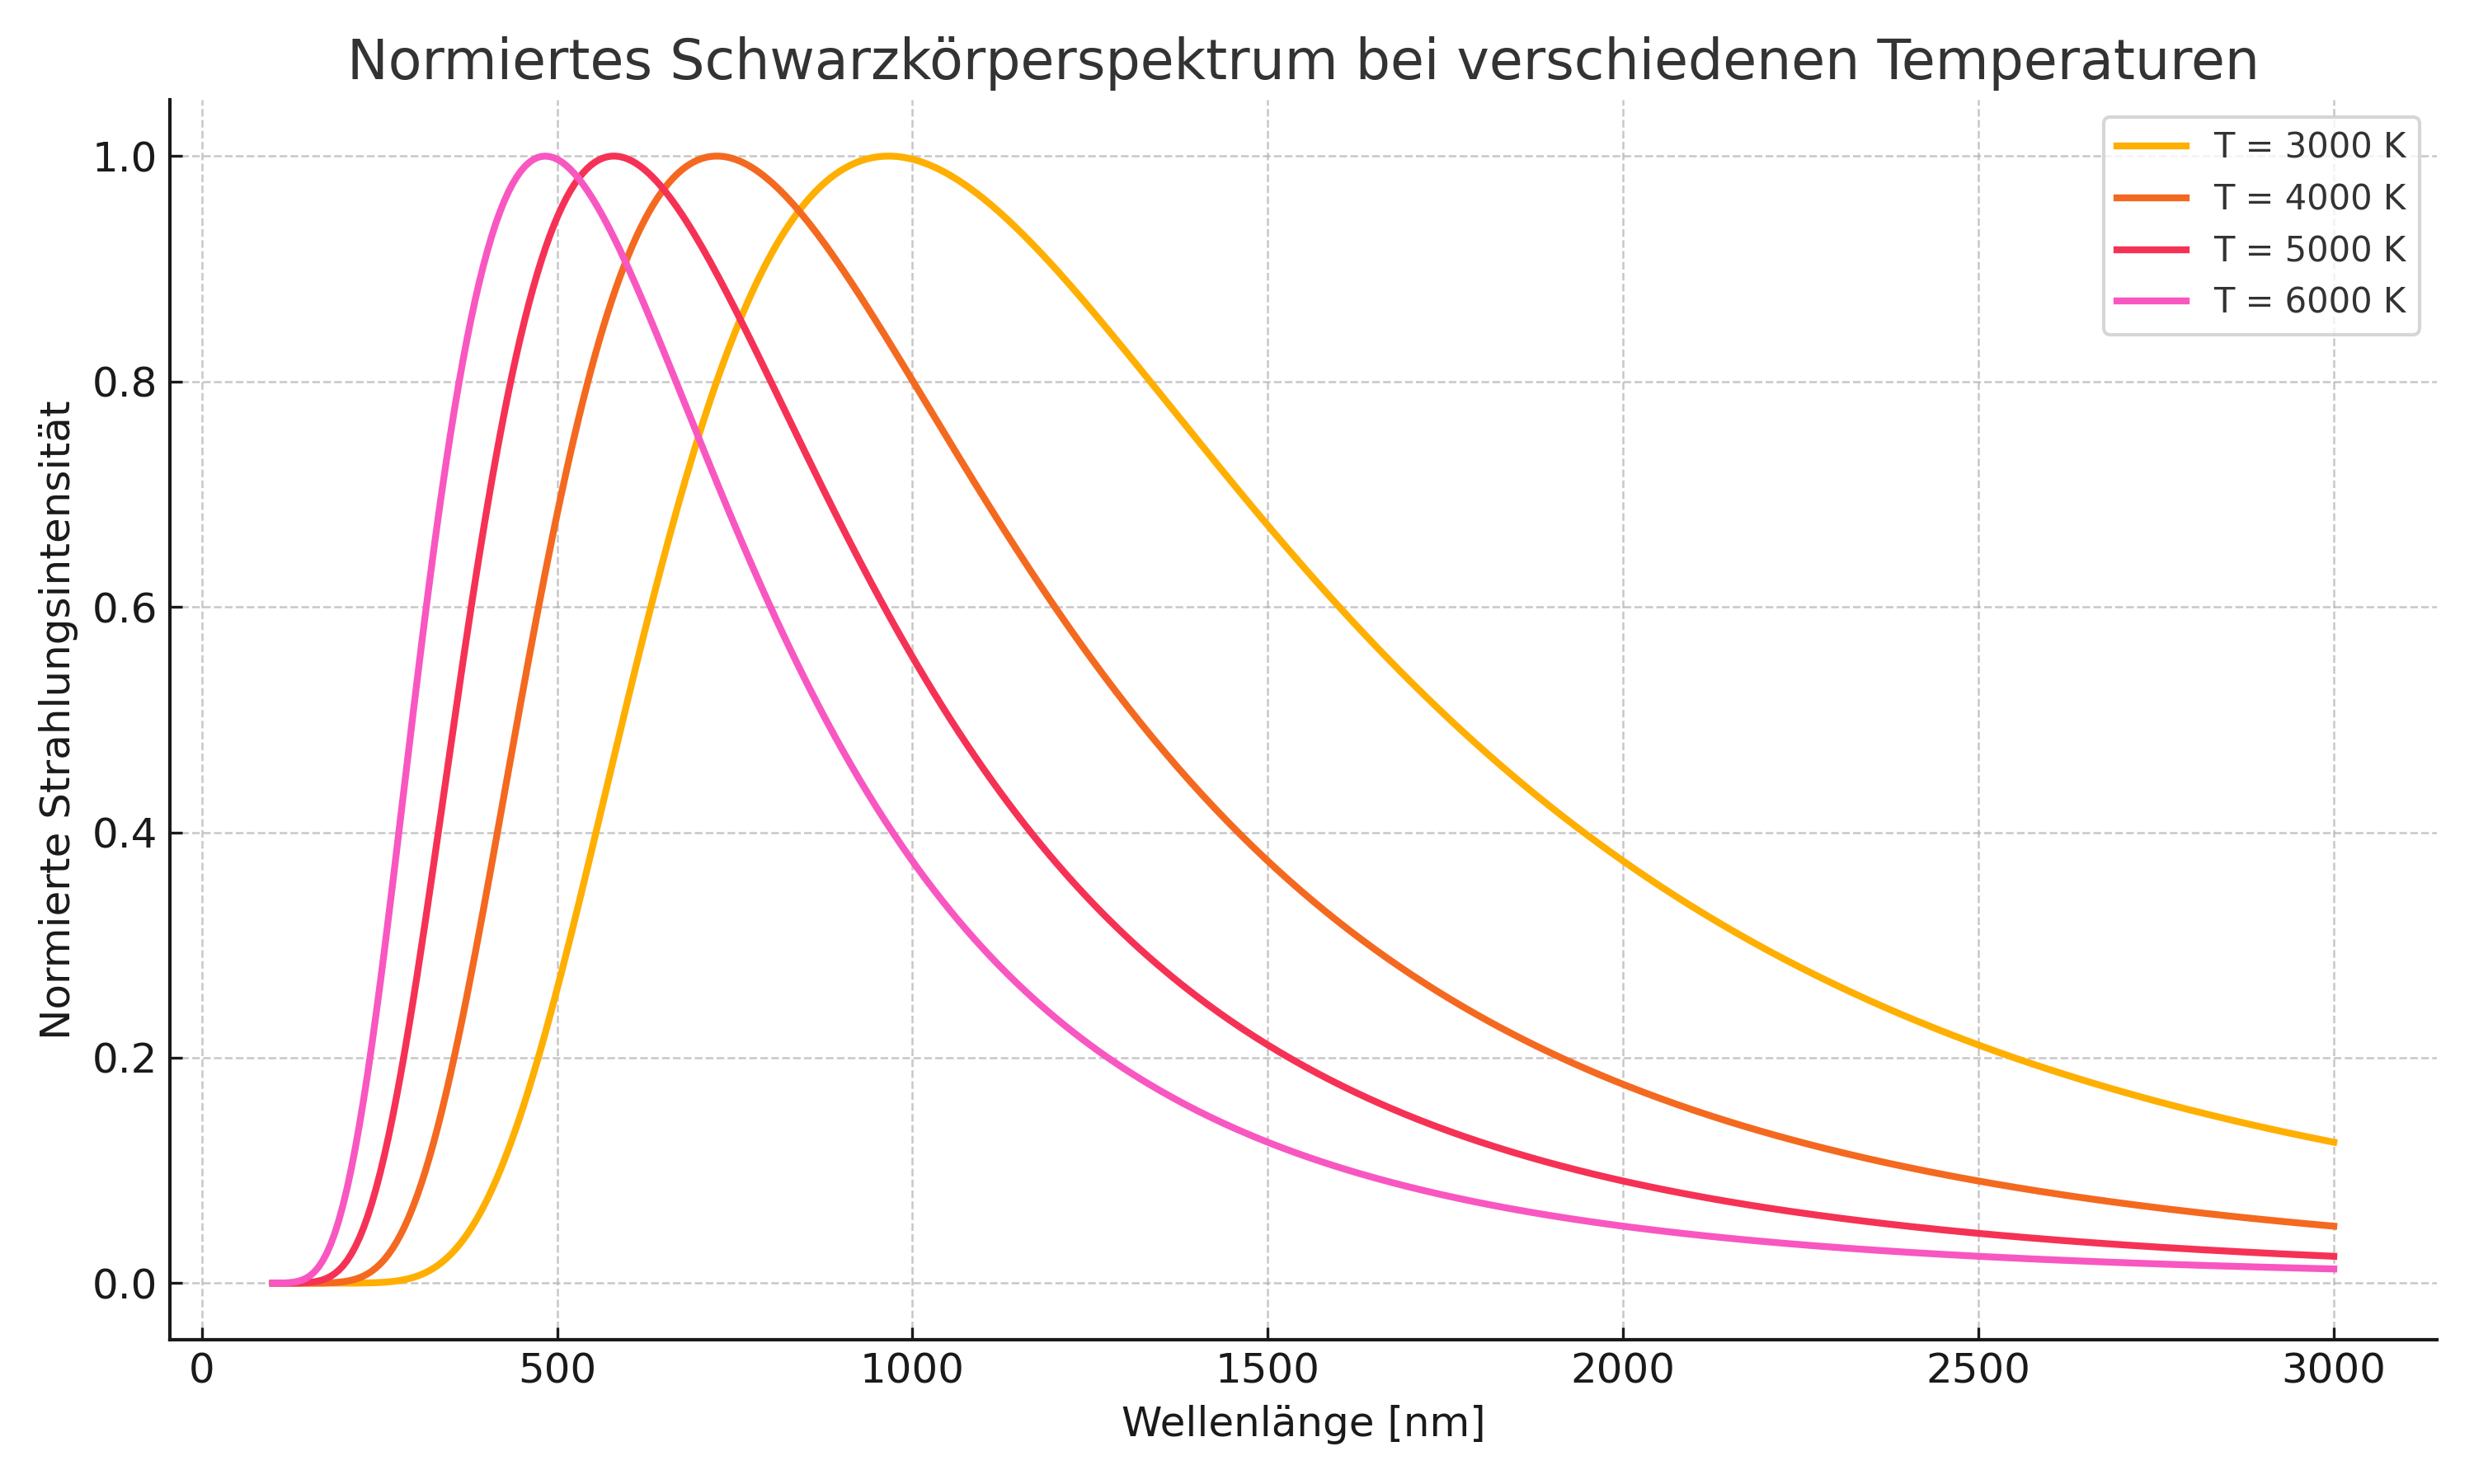
\includegraphics[width=0.85\textwidth]{bilder/schwarzer_koerper_spektrum.png}
	\caption{Normiertes Schwarzkörperspektrum für verschiedene Temperaturen. Das Maximum verschiebt sich mit zunehmender Temperatur zu kürzeren Wellenlängen (Wiensches Verschiebungsgesetz).}
	\label{fig:schwarzerkoerper}
\end{figure}

\subsubsection{Ablauf des Hohlraumexperiments}

Zur experimentellen Untersuchung der thermischen Strahlung verwendet man sogenannte \emph{Hohlraumstrahler}.\index{Hohlraumstrahler} Sie dienen als nahezu ideale Realisierung eines Schwarzen Körpers. Die typische Anordnung besteht aus einem massiven Metallblock mit einem inneren Hohlraum und einer kleinen Öffnung zur Außenwelt.
Strahlung, die durch diese Öffnung in das Innere gelangt, wird dort vielfach an den Wänden reflektiert und nahezu vollständig absorbiert. Umgekehrt tritt aus der Öffnung ein winziger Teil der inneren Gleichgewichtsstrahlung aus – diese entspricht nahezu exakt der theoretischen Schwarzkörperstrahlung bei der Temperatur \( T \) des Blocks.
Die aus der Öffnung austretende Strahlung wird mit einem Spektrometer untersucht.\index{Spektrometer} Dabei zeigt sich das typische Schwarzkörperspektrum: ein intensitätsabhängiger Verlauf mit einem Maximum, das sich mit der Temperatur verschiebt (Wiensches Verschiebungsgesetz), und ein charakteristischer Abfall im UV-Bereich. Diese Ergebnisse widersprachen der klassischen Physik fundamental und führten letztlich zur Entwicklung der Quantentheorie.

\begin{figure}[H]
	\centering
	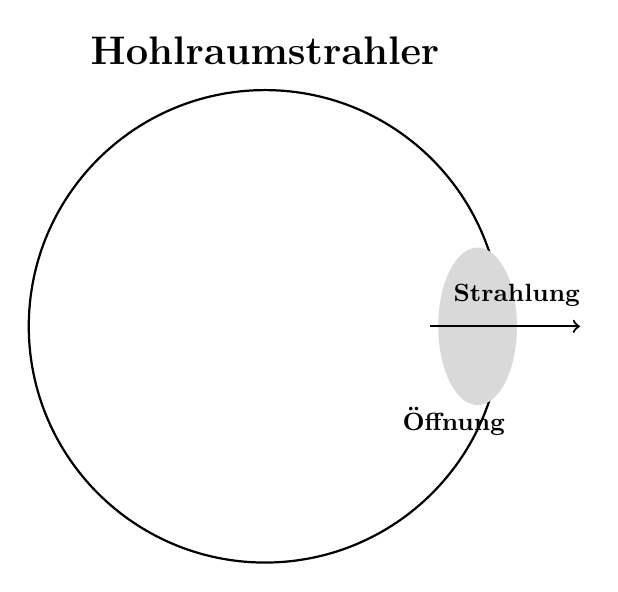
\begin{tikzpicture}
		% Hohlkörper
		\draw[thick] (0,0) circle(3);
		% Öffnung (rechts)
		\fill[gray!30] (2.7,0) ellipse (0.5 and 1.0);
		% Austretende Strahlung
		\draw[->, thick] (2.1,0) -- (4,0);
		\node at (3.2,0.4) {\small \textbf{Strahlung}};
		% Labels
		\node at (2.4,-1.2) {\small \textbf{Öffnung}};
		\node at (0,3.5) {\Large \textbf{Hohlraumstrahler}};
	\end{tikzpicture}
	\caption{Modell eines Hohlraumstrahlers zur Erzeugung nahezu idealer Schwarzkörperstrahlung.}
\end{figure}
\newpage
\noindent
\subsection{Versagen der klassischen Theorie – \newline das Rayleigh-Jeans-Gesetz}\index{Rayleigh-Jeans-Gesetz}

Im 19. Jahrhundert versuchten Lord Rayleigh und Sir James Jeans,\index{Rayleigh, Lord}\index{Jeans, James} die Schwarzkörperstrahlung mithilfe der klassischen Elektrodynamik und der statistischen Mechanik zu beschreiben.\index{Statistische Mechanik} Sie betrachteten stehende elektromagnetische Wellen in einem Hohlraum als harmonische Oszillatoren und berechneten die Energieverteilung durch Anwendung des Ausrüstungsprinzips der klassischen Thermodynamik.\index{Ausrüstungsprinzip}

Das Ergebnis war das sogenannte \emph{Rayleigh-Jeans-Gesetz}, das die spektrale Energiedichte in Abhängigkeit von der Wellenlänge \( \lambda \) und der Temperatur \( T \) beschreibt:

\[
u(\lambda, T) = \frac{8 \pi k T}{\lambda^4}
\]

Hierbei ist:
\begin{itemize}
	\item \( u(\lambda, T) \) die Strahlungsenergie pro Wellenlängenintervall und Volumen,
	\item \( k \) die Boltzmann-Konstante,\index{Boltzmann-Konstante}
	\item \( T \) die absolute Temperatur.
\end{itemize}

Für lange Wellenlängen liefert die Formel sinnvolle Ergebnisse und stimmt gut mit den experimentellen Daten überein. Doch bei kurzen Wellenlängen divergiert der Ausdruck gegen unendlich – es ergibt sich eine unphysikalische, unendliche Energiedichte:

\[
\lim_{\lambda \to 0} u(\lambda, T) \to \infty
\]

Dieses Problem wurde als \emph{Ultraviolett-Katastrophe} bekannt.\index{Ultraviolett-Katastrophe} Es widersprach fundamental den experimentellen Beobachtungen (siehe Abb.~\ref{fig:schwarzerkoerper}), bei denen die Strahlung im UV-Bereich keineswegs zunimmt, sondern stark abfällt.

Diese Katastrophe offenbarte die Grenzen der klassischen Physik. Eine neue Idee war erforderlich, um die Beobachtungen zu erklären – sie kam von Max Planck.
(Der Rechenweg über Modenzählung im Hohlraum und das klassische Ausrüstungsprinzip ist in Anhang~A, Abschnitt~\ref{anhangA:rayleigh} dargestellt.)
\subsection{Versagen der klassischen Theorie - \newline das Wiensche Strahlungsgesetz}\index{Wiensches Strahlungsgesetz}

Noch vor Planck lieferte Wilhelm Wien\index{Wien, Wilhelm} 1896 eine Näherung für das Strahlungsspektrum Schwarzer Körper im kurzwelligen Bereich. Er leitete das sogenannte \emph{Wiensche Strahlungsgesetz} aus thermodynamischen Überlegungen und dimensionsanalytischen Argumenten ab – allerdings ohne die heute bekannte Quantenvorstellung.

Die spektrale Energiedichte ergibt sich in Wellenlängenform zu:

\[
u(\lambda, T) = \frac{c_1}{\lambda^5} \exp\left(-\frac{c_2}{\lambda T}\right)
\]

Dabei sind:
\begin{itemize}
	\item \( u(\lambda, T) \): Energie pro Wellenlängenintervall und Volumen,
	\item \( \lambda \): Wellenlänge,\index{Wellenlänge}
	\item \( T \): absolute Temperatur,
	\item \( c_1 = 2\pi h c^2 \), \( c_2 = \frac{hc}{k} \): Konstanten aus Planckschen Einheiten (erst später vollständig verstanden).\index{Planck-Einheiten}
\end{itemize}

Das Wiensche Gesetz beschreibt die Strahlungsverteilung im hochfrequenten Bereich (\( \lambda \to 0 \)) sehr gut und sagt dort einen exponentiellen Abfall der Intensität voraus. Im langwelligen Bereich (\( \lambda \gg 1\ \mu\mathrm{m} \)) hingegen weicht es deutlich von den Messergebnissen ab.

Wilhelm Wien erhielt 1911 den Nobelpreis für seine Beiträge zur Strahlungstheorie. Sein Gesetz war ein wichtiger Schritt hin zur vollständigen Planckschen Theorie.
(Der mathematische Herleitungsweg des Wienschen Strahlungsgesetzes ist in Anhang~A beschrieben; vgl. Abschnitt~\ref{anhangA:wien}.)
\newpage
\noindent
\vspace{1em}
\begin{tcolorbox}[didaktikbox, title=Warum versagt die klassische Theorie?]
	\label{box:klassik-versagt}
	Das Rayleigh-Jeans-Gesetz beschreibt die Wärmestrahlung bei niedrigen Frequenzen korrekt – aber bei hohen Frequenzen liefert es absurde Ergebnisse:
	
	\begin{itemize}
		\item Die Intensität steigt unbegrenzt – je höher die Frequenz, desto größer die Strahlung.
		\item Diese „ultraviolette Katastrophe“ steht im Widerspruch zu allen Beobachtungen.
		\item Die Ursache: Die klassische Physik nimmt an, dass jeder Modus im Hohlraum beliebig viel Energie aufnehmen kann.
	\end{itemize}
	
	Diese Annahme scheitert in der Realität. Erst die Quantelung der Energie – wie sie Planck eingeführt hat – erklärt, warum hohe Frequenzen unterdrückt sind.
\end{tcolorbox}

\vspace{-1.2em}

\subsection{Entstehung des planckschen Strahlungsgesetzes}\index{Plancksches Strahlungsgesetz}

Im ausgehenden 19. Jahrhundert stellte die Beschreibung der Strahlung eines schwarzen Körpers ein fundamentales Problem der theoretischen Physik dar. Empirisch war der Verlauf der spektralen Strahlungsdichte \( I(\lambda, T) \) gut bekannt, doch keine Theorie konnte das gesamte Spektrum korrekt erklären.
\newpage
\noindent
\subsubsection{Die Krise der klassischen Physik}

Die klassische Physik konnte nur Grenzfälle erklären:

\begin{itemize}
	\item Für große Wellenlängen (\(\lambda \to \infty\)) lieferte das \textbf{Rayleigh-Jeans-Gesetz}:\index{Rayleigh-Jeans-Gesetz}
	\[
	I(\lambda, T) = \frac{8\pi c}{\lambda^4} \cdot kT
	\]
	Dieses Gesetz führte bei kleinen Wellenlängen zu einer unphysikalischen Divergenz – der sogenannten \textbf{Ultraviolett-Katas\-trophe}.\index{Ultraviolett-Katastrophe}
	
	\item Für kleine Wellenlängen (\(\lambda \to 0\)) war das \textbf{Wiensche Strahlungsgesetz} bekannt:\index{Wiensches Strahlungsgesetz}
	\[
	I(\lambda, T) = c_1 \lambda^{-5} \cdot e^{-c_2/(\lambda T)}
	\]
	Es versagte jedoch im langwelligen Bereich.
\end{itemize}

\subsubsection{Plancks Interpolationsansatz}

Max Planck\index{Planck, Max} kannte beide Grenzgesetze und suchte eine mathematische Funktion, die den gesamten beobachteten Kurvenverlauf interpolieren konnte. Dies führte ihn im Oktober 1900 zu seiner berühmten Formel:
\begin{align}
	I(\lambda, T) = \frac{2hc^2}{\lambda^5} \cdot \frac{1}{e^{hc/(\lambda kT)} - 1}
\end{align}

Dabei sind:
\begin{itemize}
	\item \( h \): Plancksches Wirkungsquantum\index{Wirkungsquantum, Plancksches}
	\item \( c \): Lichtgeschwindigkeit\index{Lichtgeschwindigkeit}
	\item \( k \): Boltzmann-Konstante\index{Boltzmann-Konstante}
	\item \( T \): absolute Temperatur
\end{itemize}
\raggedbottom
(Die detaillierte Herleitung des Planckschen Strahlungsgesetzes unter Verwendung der Energiequantelung ist in Anhang~A dargestellt; vgl. Abschnitt~\ref{anhangA:planck}.)
\subsubsection{Bemerkung zur Bedeutung von \( h \)}
\raggedbottom

Planck selbst sah seine Formel zunächst als \textbf{mathematische Interpolation}, nicht als Ausdruck einer fundamentalen Naturkonstante. Er führte die Konstante \( h \) ein, um eine passende Kurve zu erhalten – ohne sich der revolutionären Konsequenzen bewusst zu sein. Erst Albert Einstein\index{Einstein, Albert} erkannte 1905 die tiefergehende Bedeutung im Rahmen seiner Lichtquantenhypothese.\\
\vspace{-0.3em}
\begin{tcolorbox}[physikbox,title={Max Planck – Wissenschaftliche Selbstbiographie \cite{planck1948}}]
	\label{box:planck-zitat}
	„Ich hatte dabei die Empfindung, daß ich gegen meinen Willen etwas Ungeheuerliches eingeführt hatte.“
\end{tcolorbox}
\vspace{1em}
\begin{tcolorbox}[mathebox, title={Plancks Strahlungsgesetz: Eine mathematische Interpolation \cite{Hoffmann2008}}]
	\label{box:planck-interpolation}
	Max Planck suchte Ende 1900 eine Funktion, die die beobachteten Strahlungskurven des Schwarzen Körpers korrekt beschreibt. Er kombinierte bekannte Grenzgesetze (Wien für hohe, Rayleigh für niedrige Frequenzen) und entwickelte eine Interpolationsformel, die später als plancksches Strahlungsgesetz bekannt wurde:
	
	\begin{align}
		I(\nu, T) = \frac{8\pi \nu^2}{c^3} \cdot \frac{h\nu}{e^{h\nu/kT} - 1}
	\end{align}
	
	Dabei war ihm selbst die tiefere Bedeutung der eingeführten Konstante \( h \) zunächst nicht bewusst – sie diente ihm als mathematisches Hilfsmittel. Erst Einstein deutete 1905 mit seiner Lichtquantenhypothese diese Formel als Hinweis auf eine fundamentale Quantisierung der Natur.
\end{tcolorbox}
\subsubsection{Wichtige geschichtliche Erkenntnis}
\vspace{1em}
\begin{tcolorbox}[didaktikbox,title=Wichtige geschichtliche Erkenntnis {\cite{Hoffmann2008}}]
	\label{box:geschichte-planck}
	Am 14. Dezember 1900 stellte Max Planck der Physikalischen Gesellschaft seine berühmte Strahlungsformel vor. Dieser Tag gilt heute als der \textit{„Geburtstag der Quantenphysik“}. Doch weder Planck noch seine Zuhörer erkannten damals die Tragweite der Entdeckung.
	
	\medskip
	
	\textbf{Zitat:} 
	\begin{quote}
		„Obwohl keinem der anwesenden Wissenschaftler – Planck eingeschlossen – die Bedeutung und Tragweite der Formel oder der Konstanten bewusst war. Man sah in Plancks Ergebnis zunächst eine Formel, die die Strahlungsverhältnisse korrekt darstellte.“
	\end{quote}
	
	Wie Hoffmann herausstellt, wurde die Revolution erst durch Einsteins Lichtquantenhypothese (1905) und die kritische Analyse des planckschen Gesetzes durch Einstein und Ehrenfest deutlich. Planck selbst sprach erst Jahre später von einem fundamentalen Umbruch.
\end{tcolorbox}
\index{Quantenphysik}

\subsubsection{Graphische Darstellung der drei Strahlungsgesetze}

Die folgende Abbildung zeigt die spektrale Energiedichte schwarzer Körper in Abhängigkeit von der Wellenlänge. Sie vergleicht das klassische Rayleigh-Jeans-Gesetz, das Wiensche Strahlungsgesetz und das vollständige Plancksche Gesetz. Die Grafik macht deutlich:

\begin{itemize}
	\item Das Rayleigh-Jeans-Gesetz divergiert im UV-Bereich.
	\item Das Wiensche Gesetz trifft nur im kurzwelligen Bereich zu.
	\item Nur das Plancksche Gesetz beschreibt das gesamte Spektrum korrekt.
\end{itemize}

\begin{figure}[H]
	\centering
	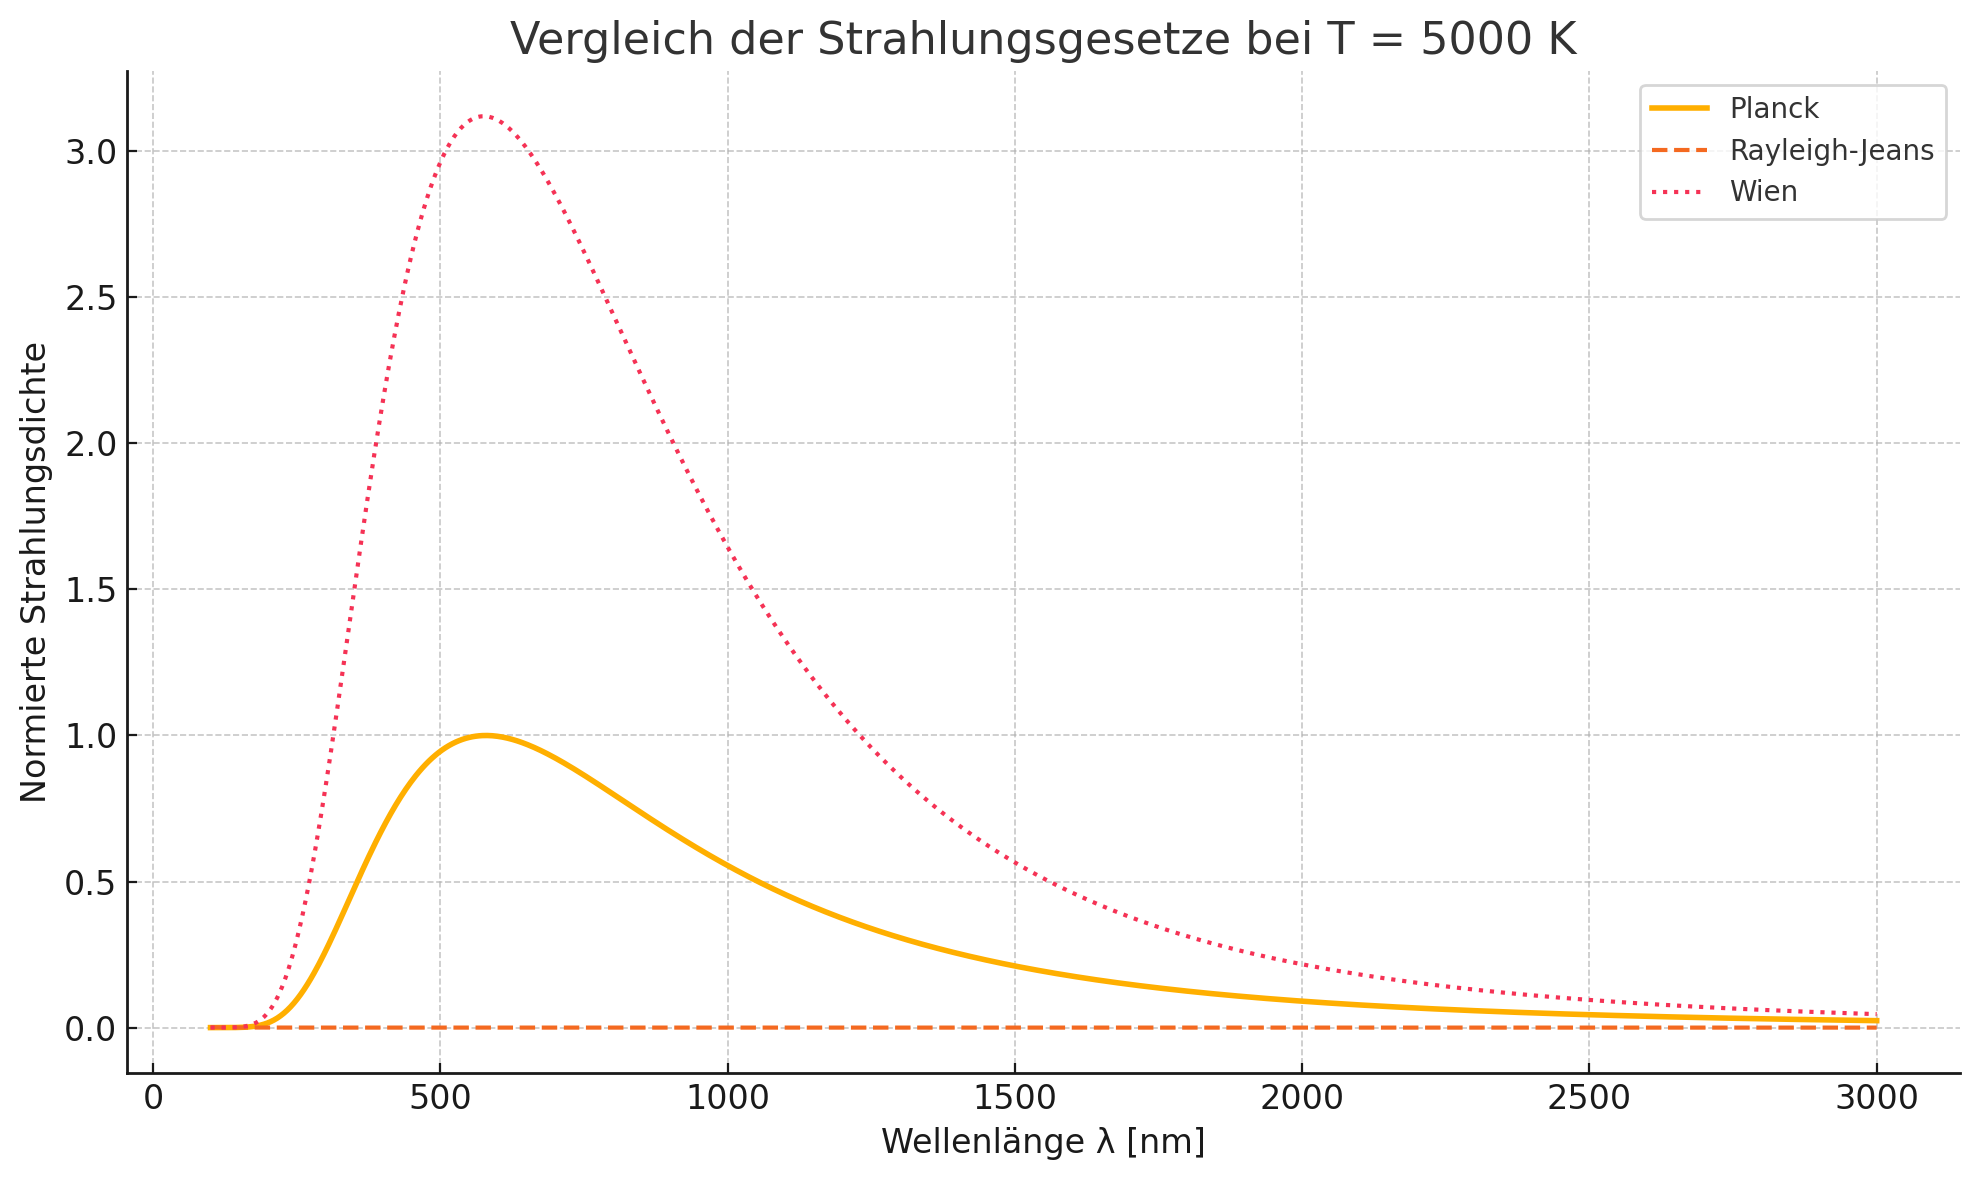
\includegraphics[width=0.85\textwidth]{bilder/strahlungsgesetze.png}
	\caption{Vergleich der drei Strahlungsgesetze. Nur das Plancksche Gesetz stimmt im gesamten Bereich mit den experimentellen Daten überein.}
	\label{fig:strahlungsgesetze}
\end{figure}

\subsubsection{Fazit}

\begin{itemize}
	\item Der Fehler der klassischen Theorie ist nicht nur groß, sondern katastrophal.
	\item Die Abweichung bei kurzen Wellen beträgt mehrere Größenordnungen.
	\item Nur das Plancksche Gesetz erklärt das gesamte Spektrum korrekt – durch die Quantisierung der Energie.
\end{itemize}

\subsection{Der Photoeffekt und Einsteins Lichtquant}\index{Photoeffekt}

Einstein ging 1905 weiter: Nicht nur die Energieabgabe, sondern das Licht selbst sei gequantelt. Er postulierte, dass ein Lichtquant (Photon) die Energie \( E = h\nu \) trägt.\index{Einstein, Albert} Nur wenn diese Energie größer ist als die Austrittsarbeit \( A \), kann ein Elektron emittiert werden:  
\[
E_{\text{kin}} = h\nu - A
\]
Dies erklärt experimentelle Beobachtungen, die mit der Wellentheorie nicht vereinbar sind – etwa die Frequenzabhängigkeit der Elektronenenergie.\index{Austrittsarbeit}

\begin{tcolorbox}[physikbox, title={Einstein (1905)\cite{einstein_lichtquanten}}]
	\label{box:einstein-lichtquant}
	„Die Entstehung von Licht erfolgt nicht überall auf der Wellenfront gleichmäßig, sondern nur an bestimmten Orten, an einzelnen Punkten.“\
	
	
	\textbf{Kommentar:} Einstein beschreibt hier bereits die Quantelung von Licht – der Startpunkt der Photonentheorie.
\end{tcolorbox}
\vspace{1em}
\index{Lichtquantenhypothese}
(Eine detaillierte Herleitung der Photoeffekt-Gleichung findet sich in Anhang~A, Abschnitt~\ref{anhangA:photoeffekt}.)
\subsection{Erste Reaktionen und Bedeutung}

Die Vorstellung, dass Licht nicht nur Wellen- sondern auch Teilcheneigenschaften besitzt, war für viele Physiker zu Beginn des 20. Jahrhunderts schwer akzeptabel. Die Wellentheorie des Lichts war durch Interferenz- und Beugungsexperimente sowie Maxwells Elektrodynamik scheinbar vollständig bestätigt.\index{Wellentheorie des Lichts} Albert Einsteins Lichtquantentheorie von 1905 – die radikale These, dass Licht aus diskreten Energiepaketen (später \emph{Photonen} genannt) besteht – widersprach dieser etablierten Sichtweise.

Einstein selbst war sich der Sprengkraft seiner Hypothese bewusst und nannte sie einen „heuristischen Gesichtspunkt“. Doch das Konzept war mehr als nur ein Rechenkniff – es erklärte den photoelektrischen Effekt vollständig und führte zu präzisen, experimentell überprüfbaren Vorhersagen.

Ein bemerkenswertes Beispiel für die anfängliche Skepsis war Robert A. Millikan.\index{Millikan, Robert A.} Obwohl er selbst 1916 in einer Reihe von Experimenten die Energieformel \( E = h \nu \) mit hoher Genauigkeit bestätigte, blieb er dem Konzept des Lichtquants lange kritisch gegenüber:

Erst nach Jahrzehnten setzte sich die Lichtquantenhypothese als fundamentaler Bestandteil der Quantenphysik durch – insbesondere nachdem auch Phänomene wie die \emph{Compton-Streuung} (1923) die Impulsnatur des Photons bestätigten.\index{Compton-Streuung}
\newpage
\noindent
Die Einführung des Photons revolutionierte nicht nur die Optik, sondern war auch entscheidend für:
\begin{itemize}
	\item die Entwicklung der \emph{Quantenmechanik},\index{Quantenmechanik}
	\item das Verständnis von \emph{Atomen und Molekülen},\index{Atom}\index{Molekül}
	\item die Theorie der \emph{Quantenelektrodynamik (QED)},\index{Quantenelektrodynamik (QED)}
	\item sowie für zahlreiche \emph{technologische Anwendungen} (Laser, Photodetektoren, Solarzellen, Quantencomputer).\index{Laser}\index{Photodetektor}\index{Solarzelle}\index{Quantencomputer}
\end{itemize}

Heute ist das Photon nicht nur ein theoretisches Konstrukt, sondern ein reales, in zahllosen Experimenten nachgewiesenes und technisch nutzbares Objekt – ein \emph{Quant der elektromagnetischen Wechselwirkung}.\index{Elektromagnetische Wechselwirkung}
\vspace{1em}
\begin{tcolorbox}[physikbox, title=Robert A. Millikan über Einstein (1916) \cite{millikan_1916}]
	\label{box:millikan-einstein}
	\emph{„Einstein’s photoelectric equation … cannot in my judgment be looked upon at present as resting upon a satisfactory theoretical foundation.“}
	
	\vspace{6pt}
	\textbf{Kommentar:} Trotz seiner experimentellen Bestätigung von Einsteins Formel lehnte Millikan das Konzept des Lichtquants zunächst ab – ein eindrucksvolles Beispiel dafür, wie tief verwurzelte theoretische Überzeugungen selbst durch klare experimentelle Befunde nicht sofort überwunden werden.
\end{tcolorbox}

\subsection{Fazit}
\vspace{1em}
\begin{tcolorbox}[hypobox, title={Was wäre, wenn nicht gequantelt wäre?}]
	\label{box:hypo-keine-quanten}
	Ohne die Annahme, dass Energie nur in diskreten Portionen ($E = nhf$) aufgenommen oder abgegeben wird:\index{Quantisierung}
	\begin{itemize}
		\item Wären fundamentale Experimente wie Schwarzkörperstrahlung und Photoeffekt unerklärbar geblieben.
		\item Wäre die klassische Physik an den Widersprüchen mit der Realität gescheitert.
		\item Hätte sich kein moderner Zugang zur Wechselwirkung von Licht und Materie entwickelt.
	\end{itemize}
	Die Quantelung war der erste Schritt zu einem neuen physikalischen Weltbild. Sie ist nicht optional – sondern grundlegend für das Verständnis des Photons.
\end{tcolorbox}


	\chapter{Eigenschaften des Photons}\index{Photon}\index{Quantenmechanik}\index{Quantenphysik}

\setcounter{section}{3}
\setcounter{subsection}{0}
\setcounter{subsubsection}{1}
\setcounter{secnumdepth}{3}
% Boxen-Stile definieren
\tcbset{physikbox/.style={colback=blue!5!white, colframe=blue!75!black, fonttitle=\bfseries}}
\tcbset{mathebox/.style={colback=green!5!white, colframe=green!50!black, fonttitle=\bfseries}}
\tcbset{didaktikbox/.style={colback=yellow!5!white, colframe=yellow!50!black, fonttitle=\bfseries}}
\tcbset{hypobox/.style={colback=orange!5!white, colframe=orange!75!black, fonttitle=\bfseries}}
\tcbset{hinweisbox/.style={colback=gray!10!white, colframe=black!40!black, fonttitle=\bfseries}}

\subsection{Photonen als Energiequanten}\index{Energiequant}

Die Vorstellung, dass Energie nicht kontinuierlich, sondern in diskreten Portionen – sogenannten Quanten – existiert, war zu Beginn des 20. Jahrhunderts revolutionär. Der Ausgangspunkt war jedoch kein bewusster physikalischer Umbruch, sondern ein mathematischer Kunstgriff von Max Planck im Jahr 1900.\index{Planck, Max}

\subsubsection{Plancks Formel als Notlösung}

Planck versuchte, das Strahlungsspektrum eines Schwarzen Körpers korrekt zu beschreiben. Um dies zu erreichen, führte er – rein formal – eine Quantisierung der Energie ein.\index{Quantisierung} Er nahm an, dass die Energieelemente, die von hypothetischen Oszillatoren aufgenommen oder abgegeben werden, ganzzahlige Vielfache einer kleinsten Energieportion der Form

\begin{equation}
	\varepsilon = h \nu
\end{equation}

sein müssten. Dabei ist:
\begin{itemize}
	\item $\varepsilon$: Energie eines Oszillators,
	\item $\nu$: dessen Schwingungsfrequenz,\index{Frequenz}
	\item $h$: das von Planck eingeführte Wirkungsquantum, $h \approx 6{,}626 \cdot 10^{-34}~\mathrm{Js}$.\index{Wirkungsquantum, Plancksches}
\end{itemize}
\newpage
\noindent
Planck selbst verstand diese Annahme jedoch nicht als Ausdruck einer realen Naturgegebenheit, sondern als eine mathematisch-statistische Hilfskonstruktion zur Ableitung der Strahlungsformel \cite{planck1948}. In seiner \emph{Wissenschaftlichen Selbstbiographie} schreibt er rückblickend:
	\vspace{1em}
\begin{tcolorbox}[physikbox, title={Max Plank (1905)\cite{planck1948}}]
	\label{box:planck1948}
	„Ich hatte mir die Strahlungsformel um jeden Preis abzuleiten vorgenommen und dies, koste es, was es wolle, auch erreicht. [...] Die Einführung eines Elementarwirkungsquantums war eine rein formale Annahme – ich wollte keineswegs eine physikalische Quantentheorie einführen.“
\end{tcolorbox}
\index{Planck, Max}

\subsubsection{Einstein macht Lichtquanten daraus}

Erst \textbf{Albert Einstein} erkannte 1905 in seiner Arbeit zum Photoeffekt, dass die Quantisierung möglicherweise keine bloße Rechenhilfe ist, sondern eine reale Eigenschaft des Lichts.\index{Einstein, Albert}\index{Photoeffekt} Er postulierte, dass Licht aus einzelnen Energiepaketen besteht – den später so genannten \emph{Photonen}. Die Energie eines solchen Photons ist gegeben durch:

\begin{equation}
	E = h \nu
\end{equation}

Damit war die Grundlage für die Quantentheorie gelegt \cite{einstein1905}.\index{Quantentheorie}

\subsubsection{Beispiele aus verschiedenen Frequenzbereichen}

Die Energie eines Photons hängt ausschließlich von seiner Frequenz $\nu$ (bzw. seiner Wellenlänge $\lambda$) ab – unabhängig von der Lichtintensität.\index{Wellenlänge}\index{Lichtintensität} Dies zeigt sich eindrucksvoll an typischen Beispielen aus Natur und Technik:

\subsubsection*{Grünes Licht}
\phantomsection
Gegeben sei die Frequenz eines typischen grünen Lichtstrahls:
\[
\nu = 6{,}0 \cdot 10^{14}~\mathrm{Hz}
\]

Die Wellenlänge ergibt sich aus dem Zusammenhang:
\[
\lambda = \frac{c}{\nu}
\]
mit der Lichtgeschwindigkeit \( c = 3{,}0 \cdot 10^8~\mathrm{m/s} \).\index{Lichtgeschwindigkeit} 
\newpage
\noindent
Also:

\[
\lambda = \frac{3{,}0 \cdot 10^8~\mathrm{m/s}}{6{,}0 \cdot 10^{14}~\mathrm{Hz}} = 5{,}0 \cdot 10^{-7}~\mathrm{m} = 500~\mathrm{nm}
\]

Nun berechnen wir die Energie eines einzelnen Photons:

\[
E = h \cdot \nu = 6{,}626 \cdot 10^{-34}~\mathrm{Js} \cdot 6{,}0 \cdot 10^{14}~\mathrm{Hz} = 3{,}976 \cdot 10^{-19}~\mathrm{J}
\]

Zur Orientierung: Diese Energiemenge ist klein, reicht aber aus, um in der Netzhaut des Auges eine chemische Reaktion auszulösen – der Beginn des Sehens.
\vspace{1em}

\begin{tcolorbox}[physikbox, title=Grünes Licht]
	\label{box:grünesLicht}
	Ein Photon grünen Lichts mit \( \nu = 6 \cdot 10^{14}~\mathrm{Hz} \) hat eine Wellenlänge von \( \lambda = 500~\mathrm{nm} \) und eine Energie von etwa \( 4 \cdot 10^{-19}~\mathrm{J} \).
\end{tcolorbox}
\index{Sichtbares Licht}

\subsubsection*{Röntgenstrahlung}
\phantomsection
Röntgenstrahlung besitzt eine extrem hohe Frequenz und entsprechend kurze Wellenlänge (im Bereich weniger Zehntel Nanometer).\index{Röntgenstrahlung} Ein einzelnes Photon trägt deutlich mehr Energie als sichtbares Licht – genug, um Elektronen aus inneren Atomschalen herauszuschlagen. Das ist die physikalische Grundlage der medizinischen Bildgebung mit Röntgenstrahlen – aber auch der Grund, warum diese Strahlung biologisch wirksam und potenziell schädlich ist.
	\vspace{1em}
\begin{tcolorbox}[physikbox, title=Röntgenstrahlen]
	\label{box:röntgenstrahlen}
	Ein Photon Röntgenstrahlung mit \( \nu = 3 \cdot 10^{18}~\mathrm{Hz} \) hat eine Wellenlänge von etwa \( \lambda = 0{,}1~\mathrm{nm} \) und eine Energie von etwa \( 2 \cdot 10^{-15}~\mathrm{J} = 12{,}4~\mathrm{keV} \).
\end{tcolorbox}

\subsubsection*{Mikrowellenstrahlung}
\phantomsection
Mikrowellen haben sehr niedrige Frequenzen und entsprechend lange Wellenlängen – typischerweise einige Zentimeter.\index{Mikrowelle} Ein einzelnes Photon trägt nur sehr wenig Energie. Diese reicht nicht aus, um Elektronen zu lösen oder chemische Reaktionen direkt auszulösen, aber sie ist genau richtig, um Wassermoleküle in Lebensmitteln zum Schwingen anzuregen. So entsteht Wärme – das physikalische Prinzip hinter Mikrowellenherden.
\vspace{1em}
\begin{tcolorbox}[physikbox, title=Mikrowellenstrahlung]
	\label{box:Mikrowellenstrahlung}
	Ein Photon typischer Mikrowellenstrahlung mit \( \nu = 2{,}45 \cdot 10^9~\mathrm{Hz} \) hat eine Wellenlänge von etwa \( \lambda = 1{,}22\cdot 10^8~\mathrm{nm} \)
	und eine Energie von etwa \( 1{,}62 \cdot 10^{-24}~\mathrm{J} \).
\end{tcolorbox}

\subsubsection{Zusammenfassung}

\begin{tcolorbox}[mathebox,title=Photonen als Energiequanten]
	\label{box:Photon als Energiequanten}
	Die Gleichung $E = h \nu$ entstand ursprünglich als mathematischer Kunstgriff zur Beschreibung der Schwarzkörperstrahlung \cite{planck1948}. Erst Einstein erkannte 1905, dass sie die reale Natur des Lichts beschreibt: Licht besteht aus diskreten Energiepaketen – Photonen \cite{einstein1905}. Dies markiert den Beginn der Quantentheorie.
\end{tcolorbox}
\index{Schwarzkörperstrahlung}
\index{Einstein, Albert}

\subsection{Impuls des Photons}\index{Impuls}

Ein wesentliches Merkmal des Photons ist sein Impuls – obwohl es keine Ruhemasse besitzt.\index{Ruhemasse} In der klassischen Mechanik ist der Impuls eines Teilchens definiert als Produkt aus Masse und Geschwindigkeit:

\[
p = m \cdot v
\]

Da Photonen masselos sind \((m_0 = 0)\), scheint diese Beziehung auf den ersten Blick nicht anwendbar. Dennoch tragen Photonen Impuls – ein Umstand, der durch Experimente wie die Compton-Streuung eindrucksvoll belegt ist.\index{Compton-Streuung} Die Erklärung liefert die Quantenphysik in Verbindung mit der speziellen Relativitätstheorie.\index{Spezielle Relativitätstheorie}

\subsubsection{Impuls aus der Quantisierung des Lichts}

Die Energie eines Photons ist gemäß Planck und Einstein gegeben durch:

\[
E = h \cdot \nu
\]
\newpage
\noindent
Gleichzeitig gilt in der Relativitätstheorie für masselose Teilchen wie das Photon der Zusammenhang:

\[
E = p \cdot c
\]

Durch Gleichsetzen erhält man den Impuls des Photons:

\[
p = \frac{E}{c} = \frac{h \cdot \nu}{c}
\]

Da die Frequenz \(\nu\) mit der Wellenlänge \(\lambda\) über \(\nu = \frac{c}{\lambda}\) verknüpft ist, ergibt sich:

\[
p = \frac{h}{\lambda} \tag{III.3}
\]

(Diese Herleitung wird in Anhang~A über die relativistische Energie-Impuls-Relation formalisiert; vgl. Abschnitt~\ref{anhangA:impuls}.)

Dieser Ausdruck zeigt: Der Impuls eines Photons ist umgekehrt proportional zu seiner Wellenlänge – je kürzer die Wellenlänge, desto größer der Impuls.
\vspace{1em}
\begin{tcolorbox}[physikbox,title=Photonenimpuls]
	\label{box:Photonenimpuls}
	Ein Photon besitzt den Impuls
	\[
	p = \frac{h}{\lambda}
	\]
	obwohl es keine Ruhemasse hat. Der Impuls steigt mit zunehmender Frequenz bzw. abnehmender Wellenlänge.
\end{tcolorbox}
\index{Photonenimpuls}

\subsubsection{Impulsübertrag in der Praxis}

Dass Licht Impuls trägt, zeigt sich z.\,B. in der Strahlungsdruckwirkung auf Materie – ein Effekt, der schon von Kepler vermutet und später experimentell bestätigt wurde.\index{Strahlungsdruck} 
\newpage
\noindent
In moderner Technik spielt der Impuls des Photons z.\,B. in folgenden Bereichen eine Rolle:

\begin{itemize}
	\item Solarsegel: Nutzung des Strahlungsdrucks zur Bewegung von Raumsonden.\index{Solarsegel}
	\begin{tcolorbox}[hinweisbox, title=Reales Bildmaterial]
		\label{keybox:RealesBildmaterial}
		Ein reales Foto des entfalteten Sonnensegels der Raumsonde \textbf{IKAROS} wurde 2010 von der Mini-Kamera \textbf{DCAM2} aufgenommen.  
		Du findest es online bei der Planetary Society unter:  
		\url{https://www.planetary.org/space-images/ikaros-spacecraft-from-dcam2}
	\end{tcolorbox}
	\item Optische Pinzetten: Manipulation kleiner Partikel mit fokussierten Lichtstrahlen.\index{Optische Pinzette}
	\begin{tcolorbox}[hinweisbox, title=Reales Bildmaterial zur optischen Pinzette]
		\label{box:Manipulation kleiner Partikel}
		Ein reales Bild und schematische Darstellung der Optischen Pinzette (Laserfalle) ist öffentlich verfügbar bei Wikipedia:  
		\url{https://en.wikipedia.org/wiki/Optical_tweezers}
	\end{tcolorbox}
\end{itemize}

\subsubsection{Zusammenhang mit De-Broglie-Wellenlänge}

Der Ausdruck \( p = \frac{h}{\lambda} \) ist nicht nur auf Photonen beschränkt, sondern gilt auch für Materiewellen (De-Broglie-Relation).\index{De-Broglie-Relation} Für massive Teilchen gilt ebenfalls:

\[
\lambda = \frac{h}{p}
\]

Damit verbindet sich der Wellencharakter mit dem Impulsbegriff – eine weitere Bestätigung des Welle-Teilchen-Dualismus auch für Licht.\index{Welle-Teilchen-Dualismus}

\subsection{Gesundheitliche Aspekte elektromagnetischer \newline Strahlung}\index{Elektromagnetische Strahlung}\index{Gesundheit}

\subsubsection{Ionisierende Strahlung: UV-Licht und darüber hinaus}

Ultraviolette Strahlung, insbesondere im Bereich unter \SI{280}{\nano\meter}, besitzt Photonen mit Energien von mehreren \si{\electronvolt}. Diese sind ausreichend, um Elektronen aus Atomen zu lösen oder chemische Bindungen aufzubrechen – man spricht von \textbf{ionisierender Strahlung}.\index{Ionisierende Strahlung}\index{Ultraviolett}

\begin{equation*}
	E = h\nu = \frac{hc}{\lambda}
	\label{eq:photonenergie}
\end{equation*}

Für UV-Licht mit einer Wellenlänge von \(\lambda = \SI{200}{\nano\meter}\) ergibt sich:

\begin{align*}
	E &= \frac{6{,}626 \cdot 10^{-34}\,\si{\joule\second} \cdot 3{,}0 \cdot 10^8\,\si{\meter\per\second}}{200 \cdot 10^{-9}\,\si{\meter}} \\
	&= \SI{9.939e-19}{\joule} \approx \SI{6.2}{\electronvolt}
\end{align*}

Diese Energie reicht aus, um DNA-Moleküle zu schädigen – ein physikalischer Mechanismus, der als Ursache von \textbf{Hautkrebs} bekannt ist.\index{DNA}\index{Hautkrebs}

\subsubsection{Nicht-ionisierende Strahlung: \newline Mobilfunk, WLAN, Mikrowellen}

Strahlung im Bereich von Funk, WLAN oder Mikrowellen hat wesentlich geringere Photonenenergien:

\begin{itemize}
	\item Mobilfunk: $\nu \approx \SI{900}{\mega\hertz} \Rightarrow E \approx \SI{3.7e-6}{\electronvolt}$
	\item WLAN: $\nu \approx \SI{2.4}{\giga\hertz} \Rightarrow E \approx \SI{1.0e-5}{\electronvolt}$
	\item Mikrowelle: $\nu \approx \SI{2.45}{\giga\hertz} \Rightarrow E \approx \SI{1.01e-5}{\electronvolt}$
\end{itemize}

Diese Energien sind \textbf{nicht ausreichend}, um ionisierende Wirkungen hervorzurufen.\index{Nicht-ionisierende Strahlung} Dennoch wird diskutiert, ob thermische oder biologische Effekte durch \textbf{kumulative Energieaufnahme} auftreten können.

\subsubsection{Zusammenfassung -- Ionisierte und  \newline Nicht-ionisierte Strahlung}
\vspace{1em}
\begin{tcolorbox}[physikbox,title=Ionisierende und Nicht-ionisierende Strahlung]
	\label{box:ionisierende}
	\begin{itemize}
		\item \textbf{Nicht-ionisierend:} Photonen besitzen zu wenig Energie, um Elektronen aus Atomen zu entfernen. Beispiele:
		\begin{itemize}
			\item Radiowellen, Mikrowellen
			\item Infrarot, sichtbares Licht
			\item Mobilfunk, WLAN, Bluetooth
		\end{itemize}
		\item \textbf{Ionisierend:} Photonen besitzen genug Energie, um Atome zu ionisieren. Dies kann Zell- oder DNA-Schäden verursachen. Beispiele:
		\begin{itemize}
			\item Ultraviolett (v.\,a.\ UV-B, UV-C)
			\item Röntgenstrahlung
			\item Gammastrahlung
		\end{itemize}
	\end{itemize}
\end{tcolorbox}
\index{Radiowellen}\index{Infrarot}\index{Sichtbares Licht}\index{Röntgenstrahlung}\index{Gammastrahlung}
\vspace{1em}
\subsubsection{Grenzwerte und Schutzmaßnahmen}

In der Praxis werden Sicherheitsgrenzwerte festgelegt, um eine übermäßige Exposition zu vermeiden. Der wichtigste Messwert ist die \textbf{Spezifische Absorptionsrate (SAR)}, gemessen in \si{\watt\per\kilogram}, die beschreibt, wie viel elektromagnetische Energie pro Kilogramm Körpergewebe absorbiert wird.\index{SAR (Spezifische Absorptionsrate)}

\begin{itemize}
	\item EU-Grenzwert für Mobilgeräte: \SI{2}{\watt\per\kilogram}
	\item WLAN-Router: meist deutlich darunter
\end{itemize}

\subsubsection{Fallstudie: UV-C-Strahlung zur Keimabtötung}

Ultraviolette Strahlung im Bereich von \SI{200}{nm} bis \SI{280}{nm} – sogenanntes \textbf{UV-C} – besitzt eine hohe Photonenenergie von bis zu \SI{6.2}{\electronvolt}.\index{UV-C} Diese reicht aus, um \textbf{DNA und RNA von Mikroorganismen direkt zu schädigen}, etwa durch Bildung von Pyrimidindimeren. Dadurch wird die Vermehrung von Bakterien und Viren wirksam unterbunden.
\newpage
\noindent
\textbf{Anwendung:}
\begin{itemize}
	\item In Krankenhäusern werden UV-C-Lampen zur Desinfektion von Oberflächen, Luft und Geräten eingesetzt.
	\item Auch in der Trinkwasseraufbereitung findet UV-C Anwendung – ohne chemische Zusätze.
\end{itemize}

\textbf{Physikalische Grundlage:}
\[
E = \frac{hc}{\lambda} = \frac{6{,}626 \cdot 10^{-34}\,\si{\joule\second} \cdot 3{,}0 \cdot 10^8\,\si{\meter\per\second}}{254 \cdot 10^{-9}\,\si{\meter}} \approx \SI{7.83e-19}{\joule} \approx \SI{4.9}{\electronvolt}
\]

Diese Energie reicht aus, um kovalente Bindungen in DNA-Molekülen aufzubrechen – ein physikalisch klar nachvollziehbarer Mechanismus der Desinfektion.
\vspace{0.5em}
\begin{tcolorbox}[physikbox, title=Hinweis zur Gefährdung]
	\label{box:Hinweis zur Gefärdung}
	UV-C-Strahlung wirkt nicht nur auf Mikroorganismen, sondern kann auch menschliche Haut und Augen schädigen. Der direkte Kontakt ist daher unbedingt zu vermeiden.
\end{tcolorbox}

\subsection{Das elektromagnetische Spektrum}\index{Elektromagnetisches Spektrum}

\subsubsection{Überblick}

Das elektromagnetische Spektrum umfasst alle Formen elektromagnetischer Strahlung – von langwelligen Radiowellen bis hin zu kurzwelligen Gammastrahlen. Die Unterscheidung erfolgt typischerweise nach Frequenz \(\nu\), Wellenlänge \(\lambda\) oder Photonenenergie \(E = h\nu = \frac{hc}{\lambda}\).
\newpage
\noindent
\subsubsection{Darstellung}

\begin{figure}[H]
	\centering
	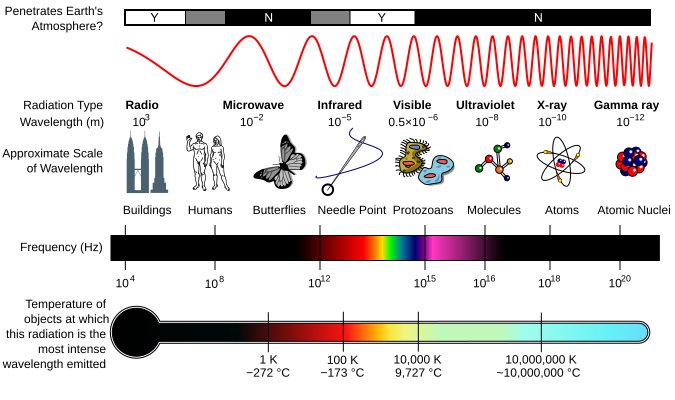
\includegraphics[width=\textwidth]{bilder/spektrum.png}
	\caption{Das elektromagnetische Spektrum mit Zuordnung typischer Anwendungen. Quelle: Wikimedia Commons}
	\label{fig:em_spektrum}
\end{figure}

\subsubsection{Frequenz-, Wellenlängen- und Energiebereiche}

\begin{table}[H]
	\centering
	\scriptsize
	\resizebox{0.95\textwidth}{!}{   % 0.95 = ca. 0,5 cm kleiner machen
		\begin{tabular}{|l|c|c|c|}
			\hline
			\textbf{\raisebox{-0.2ex}{Bereich}}& \textbf{\raisebox{-0.2ex}{Frequenz}}& \textbf{\raisebox{-0.2ex}{Wellenlänge}} &\textbf{\raisebox{-0.2ex}{Photonenenergie}}\\
			\hline
			Radiowellen      & \SI{1e3}{}–\SI{1e8}{Hz} & km – m & \(\sim\)\SI{1e-9}{eV} \\
			Mikrowellen      & \SI{1e8}{}–\SI{1e11}{Hz} & m – mm & \(\sim\)\SI{1e-6}{eV} \\
			Infrarot         & \SI{1e11}{}–\SI{4e14}{Hz} & mm – \SI{750}{nm} & \SI{1e-3}{eV} – \SI{1}{eV} \\
			Sichtbares Licht & \SI{4e14}{}–\SI{8e14}{Hz} & \SI{750}{nm} – \SI{380}{nm} & \SI{1.6}{eV} – \SI{3.3}{eV} \\
			Ultraviolett     & \SI{8e14}{}–\SI{3e16}{Hz} & \SI{380}{nm} – \SI{10}{nm} & bis \SI{100}{eV} \\
			Röntgen          & \SI{3e16}{}–\SI{3e19}{Hz} & \SI{10}{nm} – \SI{0.01}{nm} & \SI{100}{eV} – \SI{100}{keV} \\
			Gammastrahlung   & >\SI{3e19}{Hz} & < \SI{0.01}{nm} & > \SI{100}{keV} \\
			\hline
		\end{tabular}
	} % Ende resizebox
	\caption{Typische Bereiche des elektromagnetischen Spektrums mit Frequenz, Wellenlänge und Energie}
	\label{tab:spektrum}
\end{table}


\subsubsection{Einordnung von Anwendungen}

Typische Anwendungen in verschiedenen Spektralbereichen:

\begin{itemize}
	\item \textbf{Radiowellen:} Rundfunk, Funktechnik, MRT
	\item \textbf{Mikrowellen:} Mobilfunk, WLAN, Mikrowellenherd
	\item \textbf{Infrarot:} Fernbedienung, Thermografie
	\item \textbf{Sichtbar:} Optik, Fotografie, biologische Wahrnehmung
	\item \textbf{UV:} Sonnenbrand, Desinfektion (UV-C)
	\item \textbf{Röntgen:} Medizinische Bildgebung, Materialprüfung
	\item \textbf{Gamma:} Strahlentherapie, Astrophysik
\end{itemize}

\begin{tcolorbox}[hinweisbox,title=Fazit zum elektromagnetischen Spektrum]
	\label{box:Fazit zum elektro}
	\textbf{Physikalisches Fazit:}
	
	\begin{itemize}
		\item Das elektromagnetische Spektrum umfasst Wellen aller Frequenzen – von Radiowellen bis Gammastrahlen.
		\item Die Photonenenergie wächst mit zunehmender Frequenz (bzw. abnehmender Wellenlänge) gemäß \(E = h \nu = \frac{hc}{\lambda}\).
		\item Der Übergang zur \textbf{ionisierenden Strahlung} beginnt typischerweise im Bereich der UV-Strahlung, bei Photonenergien von etwa \SI{10}{\electronvolt}.
	\end{itemize}
	
	\vspace{0.5em}
	\textbf{Didaktisches Fazit:}
	
	\begin{itemize}
		\item Die Einordnung typischer Anwendungen – z.\,B. Mobilfunk, Mikrowelle, UV-Desinfektion oder Röntgendiagnostik – in das Spektrum erleichtert das Verständnis ihrer physikalischen und biologischen Wirkung.
		\item Besonders hilfreich ist die visuelle Verbindung zwischen Frequenz, Wellenlänge, Energie und biologischer Relevanz.
		\item \textbf{Merksatz:} Je kürzer die Wellenlänge, desto höher die Photonenenergie – und desto größer das Potenzial für biologische Schäden.
	\end{itemize}
\end{tcolorbox}
\newpage
\noindent
\subsection{Masselosigkeit und Bewegung mit \newline Lichtgeschwindigkeit}\index{Masselosigkeit}\index{Lichtgeschwindigkeit}

\subsubsection{Keine Ruhemasse -- aber Energie und Impuls}

Das Photon besitzt keine Ruhemasse, d.\,h. $m_0 = 0$. Dennoch ist es Tr\"ager von Energie und Impuls.\index{Energie} Die Energie eines Photons ergibt sich nach Planck und Einstein zu:
\begin{equation}
	E = h \nu
\end{equation}
Der Impuls eines Photons folgt daraus direkt:
\begin{equation}
	p = \frac{E}{c} = \frac{h\nu}{c} = \frac{h}{\lambda}
\end{equation}
Damit widerspricht das Photon nicht der Relativit\"atstheorie -- im Gegenteil: Diese Beziehungen sind genau die Konsequenz der speziellen Relativit\"at f\"ur masselose Teilchen.

\subsubsection{Was w\"are, wenn das Photon eine winzige Masse h\"atte?}

\paragraph{Relativistische Energieformel:} W\"are das Photon nicht ganz masselos, m\"usste man die allgemeine relativistische Energieformel verwenden:
\begin{equation}
	E = \gamma m_0 c^2 = \frac{m_0 c^2}{\sqrt{1 - \frac{v^2}{c^2}}}
\end{equation}
Dann g\"alte auch f\"ur den Impuls:
\begin{equation}
	p = \gamma m_0 v
\end{equation}
Die einfache Beziehung $E = pc$ w\"are dann nicht mehr korrekt, sondern es m\"usste gelten:
\begin{equation}
	E^2 = (pc)^2 + (m_0 c^2)^2
\end{equation}

(Eine mathematisch detaillierte Darstellung der Energie-Impuls-Relation für masselose und hypothetisch massive Photonen findet sich in Anhang~A, Abschnitt~\ref{anhangA:masse}.)
\newpage
\noindent
\subsubsection*{Physikalische Konsequenzen:}
\phantomsection
\begin{itemize}
	\item Die Lichtgeschwindigkeit w\"are nicht mehr konstant f\"ur alle Photonen.
	\item Die Geschwindigkeit h\"ange von der Energie (bzw. Frequenz) ab $\Rightarrow$ Verletzung der Lorentz-Invarianz.
	\item Langwelliges Licht w\"urde langsamer als kurzwelliges.
	\item Das Coulomb-Gesetz m\"usste modifiziert werden $\Rightarrow$ Reichweite der elektrischen Kraft endlich.
\end{itemize}

\paragraph{Experimentelle Grenzen:}
Pr\"azise Messungen zeigen: Wenn das Photon eine Masse besitzt, dann ist sie extrem klein:
\begin{equation}
	m_\gamma < 10^{-54} \text{ kg} \approx 10^{-18} \text{ eV}/c^2
\end{equation}
\index{Photonenmasse}

\textbf{Die Zahl} $10^{-54} \text{ kg}$ 	\textbf{ist kein Naturgesetz und auch kein theoretischer Wert}, sondern eine Obergrenze, die sich aus dem Ergebnis vieler Experimente und Beobachtungen ergibt – unter der Annahme, dass das Photon eine Masse haben könnte.
Solche winzigen Abweichungen konnten bisher nicht experimentell festgestellt werden.

\begin{figure}[H]
	\centering
	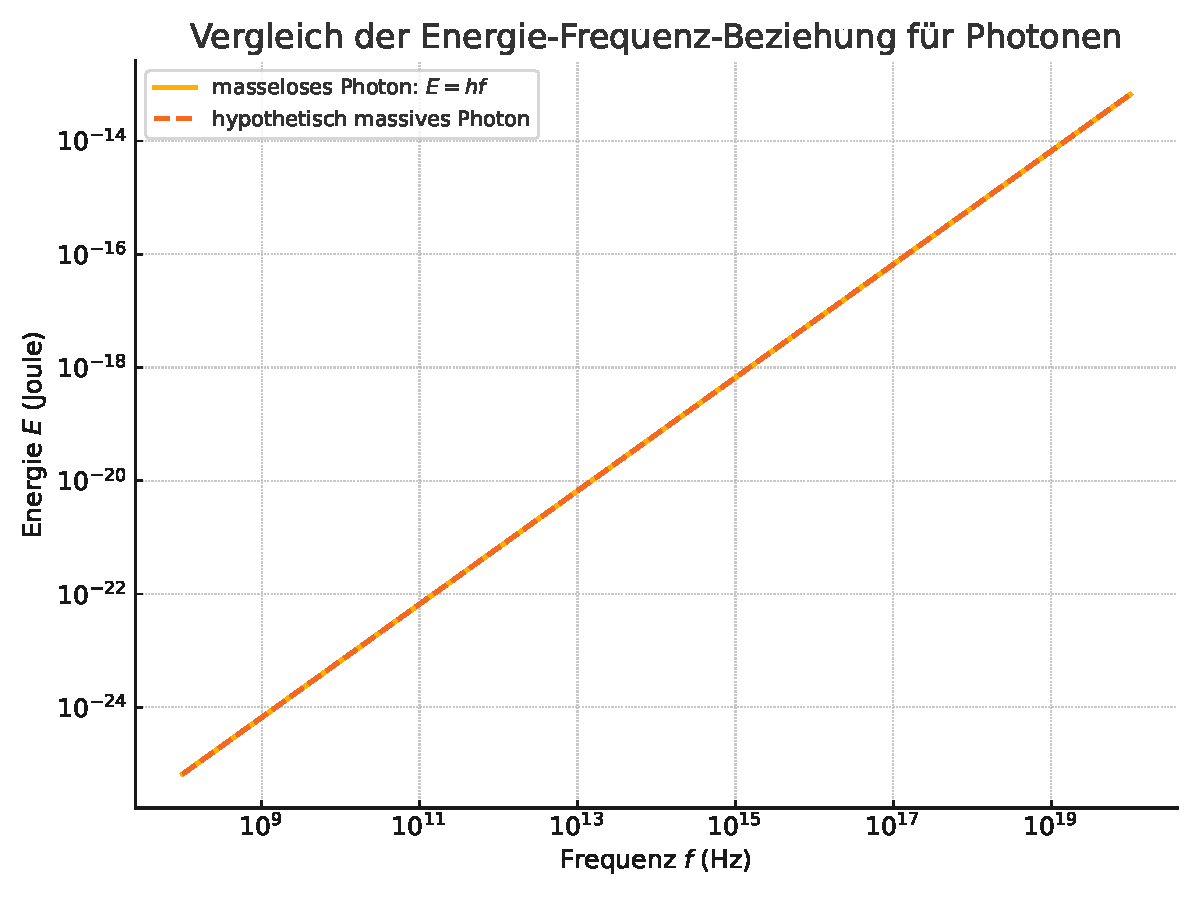
\includegraphics[width=0.85\textwidth]{bilder/photon_energie_vergleich_didaktisch.pdf}
	\caption{Didaktischer Vergleich der Energie-Frequenz-Beziehung \( E(f) \) für ein masseloses Photon (blau) und ein hypothetisch massives Photon mit überhöhter Masse (rot gestrichelt). }
	\label{fig:energie_f_masselos_massiv}
\end{figure}
\vspace{1em}
\begin{tcolorbox}[hinweisbox, title=Hinweis zur Grafik: Warum sieht man keinen Unterschied?]
	\label{box:Warum sieht man}
	Die Energie-Frequenz-Beziehung $E(f)$ wurde grafisch f\"ur masselose und hypothetisch massereiche Photonen dargestellt. Aufgrund der extrem kleinen experimentellen Obergrenze f\"ur die Photonenmasse ($m_\gamma < 10^{-54}$ kg) unterscheiden sich die beiden Kurven selbst im Log-Log-Diagramm praktisch nicht. \\[1ex]
	\textbf{Genau diese fehlende Abweichung ist ein starker Hinweis auf die Masselosigkeit des Photons.}
\end{tcolorbox}
\vspace{1em}
\begin{tcolorbox}[hypobox, title={Was wäre wenn, wenn das Photon eine Masse hätte? }]
	\label{box:was wäre wenn}
	Wenn das Photon eine auch nur winzige Masse hätte ($m_\gamma > 0$), dann:
	\begin{itemize}
		\item Würde es sich langsamer als Lichtgeschwindigkeit bewegen ($v < c$),
		\item Wäre die Energie-Frequenz-Beziehung nicht mehr $E = hf$, sondern:
		\begin{equation*}
			E = \sqrt{(hf)^2 + (m_\gamma c^2)^2}
		\end{equation*}
		\item Wäre die Lichtgeschwindigkeit nicht mehr konstant – z.\,B. würde langwelliges Licht langsamer laufen als kurzwelliges,
		\item Würde sich das Coulomb-Gesetz \textit{abschneiden} – die Reichweite elektrischer Felder wäre endlich.
	\end{itemize}
	Da all dies nicht beobachtet wird, gilt: Das Photon ist mit höchster Wahrscheinlichkeit wirklich masselos.
\end{tcolorbox}
\vspace{1em}
\newpage
\noindent
\subsubsection{Warum w\"urde \( E = h f \) bei massereichem Photon nicht mehr gelten?}

Die Formel $E = hf$ gilt nur exakt f\"ur masselose Teilchen. W\"are das Photon massereich, m\"usste gelten:
\begin{equation}
	E = \sqrt{(hf)^2 + (m_\gamma c^2)^2} > hf
\end{equation}
Die Energie hinge nicht mehr nur von der Frequenz ab -- und das w\"are experimentell messbar.

\paragraph{Best\"atigte Experimente:}
\begin{itemize}
	\item Photoeffekt
	\item Compton-Effekt
	\item Spektrallinien und Laserspektroskopie
	\item Quantenoptik und QED-Experimente
\end{itemize}
Alle best\"atigen mit hoher Pr\"azision die Beziehung $E = hf$. Eine systematische Abweichung wurde nie gefunden.
\vspace{1em}
\begin{tcolorbox}[physikbox, title=Fazit: Warum das Photon masselos ist]
	\begin{itemize}
		\label{box:Warum das Photon}
		\item Das Photon hat keine Ruhemasse ($m_0 = 0$), aber Energie und Impuls.
		\item Es bewegt sich zwingend mit Lichtgeschwindigkeit:\newline $v = c$.
		\item Nur unter dieser Bedingung gilt $E = pc$ und $E = hf$.
		\item W\"are $m_\gamma > 0$, w\"urde das gegen viele Beobachtungen und die spezielle Relativit\"at versto\"sen.
	\end{itemize}
\end{tcolorbox}
\vspace{1em}
\newpage
\noindent
\subsection{Spin und Polarisation}\index{Spin}\index{Polarisation}\index{Boson}\index{Helizität}

\subsubsection{Spin des Photons}

In der Quantenmechanik ist der \textbf{Spin} eine fundamentale Eigenschaft von Elementarteilchen – vergleichbar mit einem intrinsischen Drehimpuls. Anders als der klassische Drehimpuls bezieht sich der Spin nicht auf eine tatsächliche Rotation im Raum, sondern ist eine rein quantenmechanische Größe mit diskreten Werten.

\vspace{0.5em}
\textbf{Photonen besitzen den Spin 1}, gehören also zur Klasse der sogenannten \textit{Bosonen}. Während Teilchen mit halbzahligem Spin (wie Elektronen mit Spin $1/2$) den Fermionen zugeordnet werden und dem Pauli-Prinzip unterliegen, dürfen Bosonen denselben Quantenzustand einnehmen – ein Prinzip, das für Lichtteilchen fundamentale Konsequenzen hat, z.\,B. bei der Verstärkung von Laserlicht.\index{Fermion}\index{Pauli-Prinzip}\index{Laser}
\vspace{1em}
\begin{tcolorbox}[physikbox, title=Eigenschaften des Photon-Spins]
	\label{box:Eigenschaften des}
	\begin{itemize}
		\item Photonen haben \textbf{Spin 1}, aber keine Ruhemasse.
		\item Es gibt nur zwei messbare Spin-Zustände: \textbf{Helizität $+1$ und $-1$}.
		\item Die \textbf{Spinrichtung} liegt stets entlang der Bewegungsrichtung des Photons.
	\end{itemize}
\end{tcolorbox}
\vspace{1em}
Der Grund für die Beschränkung auf nur zwei Spin-Zustände liegt in der \textbf{Masselosigkeit des Photons}. Im Gegensatz zu massiven Spin-1-Teilchen (wie etwa dem Z-Boson) existiert für das Photon keine Ruhemasse, und somit auch kein Ruhesystem. Dadurch entfällt die Möglichkeit eines longitudinalen Spin-Zustands (Spin-0-Komponente), wie sie bei massiven Teilchen auftritt. Übrig bleiben nur die beiden Transversalmoden mit Helizität $\pm1$.\index{Z-Boson}

(Eine formale Herleitung der zulässigen Helizitätszustände des Photons findet sich in Anhang~A, Abschnitt~\ref{anhangA:helizitaet}.)

\newpage
\noindent
\textbf{Helizität} bezeichnet die Projektion des Spins auf die Bewegungsrichtung des Teilchens. Für Photonen bedeutet dies:
\begin{itemize}
	\item \textbf{Helizität $+1$}: Rechtszirkular polarisiertes Licht.
	\item \textbf{Helizität $-1$}: Linkszirkular polarisiertes Licht.
\end{itemize}

\begin{figure}[H]
	\centering
	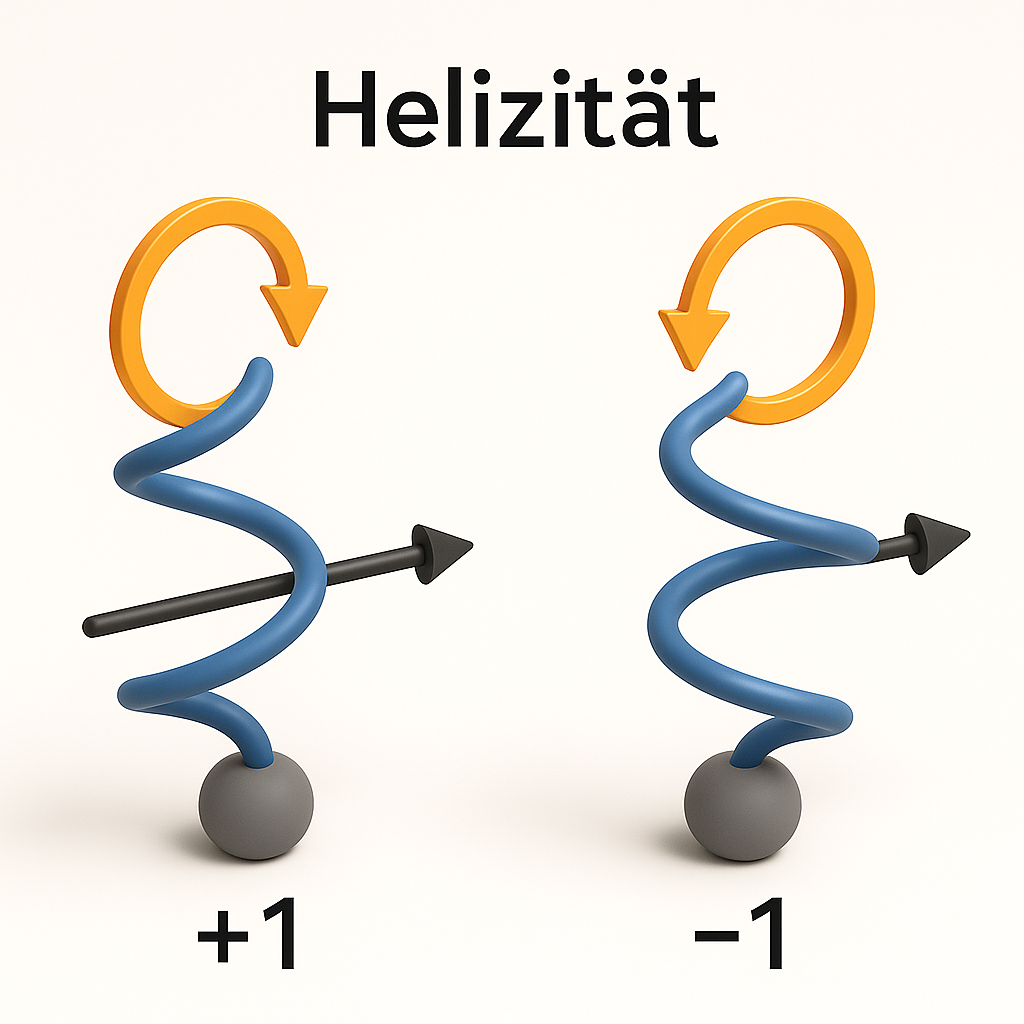
\includegraphics[width=0.65\textwidth]{bilder/Helizitaet.png}
	\caption{Visualisierung der Helizität eines Photons. Links: Helizität $+1$ (rechtszirkular), rechts: Helizität $-1$ (linkszirkular). Die orangefarbenen Pfeile zeigen die Drehrichtung (Spin), die schwarzen Pfeile die Ausbreitungsrichtung des Photons.}
	\label{fig:helizitaet}
\end{figure}

\begin{tcolorbox}[physikbox, title=Kommentar zur Darstellung]
	\label{box:Kommentar zur Darstellung}
	Die spiralförmige Struktur veranschaulicht, wie sich der elektrische Feldvektor bei zirkular polarisierter Strahlung dreht. Das Photon bewegt sich geradlinig entlang der Ausbreitungsrichtung (Impulspfeil). Die gezeigte Spirale stellt die Rotation des Feldes dar – nicht den Flugweg. Dies ist eine wichtige Unterscheidung beim Verständnis von Helizität.
\end{tcolorbox}
\vspace{1em}
Diese beiden Zustände bilden die quantenmechanische Grundlage für die \textit{zirkulare Polarisation}, auf die wir im nächsten Abschnitt näher eingehen.

\newpage
\noindent
Zum Vergleich:
\begin{itemize}
	\item Ein \textbf{Elektron} besitzt Spin $1/2$ mit zwei Zuständen (up/down).
	\item Ein \textbf{Z-Boson} (massiv, Spin 1) zeigt drei Zustände: $-1$, $0$, $+1$.
	\item Das \textbf{Photon} (masselos, Spin 1) zeigt nur $-1$ und $+1$ – der $0$-Zustand entfällt.
\end{itemize}
\vspace{1em}
\begin{tcolorbox}[physikbox, title=Didaktischer Merksatz]
	\label{box:didaktischerMerksatz}
	Masselose Spin-1-Teilchen wie Photonen besitzen nur zwei mögliche Helizitätszustände: \textbf{$\pm1$}. Der longitudinal gepolte Zustand mit $0$ existiert nicht, weil sich kein Ruhesystem definieren lässt.
\end{tcolorbox}
\vspace{1em}
\subsubsection*{Fazit}
\phantomsection
Der Spin des Photons unterscheidet sich grundlegend vom Spin massiver Teilchen. Als masseloses Spin-1-Teilchen besitzt das Photon nur zwei mögliche Helizitätszustände: +1 und -1. Ein longitudinaler Spin-Zustand mit Helizität 0 ist ausgeschlossen, da kein Ruhesystem existiert.

\vspace{0.5em}
Die Rotation des Spins kann daher nur entlang der Bewegungsrichtung betrachtet werden – sie äußert sich in der Helizität:

\begin{itemize}
	\item Helizität +1: Spin zeigt in Bewegungsrichtung (rechtszirkular)
	\item Helizität -1: Spin zeigt entgegen der Bewegungsrichtung (linkszirkular)
\end{itemize}

Der klassische Begriff einer realen Rotation ist hier nicht anwendbar. Der Spin ist eine intrinsische quantenmechanische Eigenschaft, die sich beim Photon als zirkulare Polarisation zeigt.

\subsubsection{Polarisation als makroskopische Erscheinung \newline des Spins}

Die Polarisation von Licht ist ein beobachtbares Phänomen, das direkt mit dem quantenmechanischen Spin des Photons verknüpft ist. Während der Spin eine intrinsische Eigenschaft jedes einzelnen Photons darstellt, beschreibt die Polarisation den kollektiven Zustand eines Lichtfeldes – also vieler Photonen gemeinsam.

\vspace{0.5em}
Klassisch versteht man unter Polarisation die Ausrichtung des elektrischen Feldvektors einer elektromagnetischen Welle. Dieser schwingt stets senkrecht zur Ausbreitungsrichtung, kann jedoch verschiedene Richtungen und Rotationen annehmen:

\begin{itemize}
	\item \textbf{Linear polarisiertes Licht:} Der elektrische Feldvektor schwingt in einer festen Richtung (z.\,B. vertikal oder horizontal).
	\item \textbf{Zirkular polarisiertes Licht:} Der elektrische Feldvektor rotiert mit konstanter Amplitude im Kreis – im Uhrzeigersinn (rechtszirkular) oder gegen den Uhrzeigersinn (linkszirkular).
	\item \textbf{Elliptisch polarisiertes Licht:} Allgemeinster Fall – der Feldvektor beschreibt eine Ellipse.
\end{itemize}
\index{Linear polarisiertes Licht}\index{Zirkular polarisiertes Licht}\index{Elliptisch polarisiertes Licht}

\vspace{0.5em}
In der Quantenoptik entspricht die Polarisation dem kollektiven Zustand der Helizitäten vieler Photonen.\index{Quantenoptik} Ein vollständig rechtszirkular polarisiertes Lichtfeld besteht aus Photonen mit Helizität +1, linkszirkular polarisiertes Licht aus Photonen mit Helizität -1. Lineare Polarisation entsteht aus einer quantenmechanischen Überlagerung beider Zustände:

\begin{equation}
	|\text{linear}\rangle = \frac{1}{\sqrt{2}} \left( |+1\rangle + |-1\rangle \right)
\end{equation}

(Eine ausführlichere Darstellung der Polarisation in der Dirac-Notation und mit Jones-Vektoren findet sich in Anhang~A, Abschnitt~\ref{anhangA:polarisation}.)
\vspace{1em}
\begin{tcolorbox}[physikbox, title=Superposition und Polarisation]
	\label{box:Superposition}
	Ein linear polarisiertes Photon ist ein quantenmechanischer Überlagerungszustand der beiden Helizitätszustände $|+1\rangle$ und $|-1\rangle$. Diese Superposition führt zur festen Schwingungsrichtung des elektrischen Feldes.
\end{tcolorbox}

\vspace{0.5em}
Damit stellt die Polarisation eine direkt beobachtbare Konsequenz des Photon-Spins dar. In vielen Experimenten – z.\,B. mit Polarisationsfiltern, Polarisationskameras oder im Doppelspaltversuch mit polarisierter Strahlung – zeigt sich die Polarisation als makroskopisch messbares Phänomen quantenmechanischer Ursprünge.\index{Polarisationsfilter}
\vspace{1em}
\begin{tcolorbox}[physikbox, title=Superposition und Polarisation]
	\label{box:Superposition und Polarisation}
	Ein linear polarisiertes Photon befindet sich in einem quantenmechanischen Überlagerungszustand der beiden Helizitätszustände $|+1\rangle$ (rechtszirkular) und $|-1\rangle$ (linkszirkular):
	
	\[
	|\text{linear}\rangle = \frac{1}{\sqrt{2}} \left( |+1\rangle + |-1\rangle \right)
	\]
	
	Diese Superposition bedeutet:
	\begin{itemize}
		\item Das Photon besitzt keine definierte Helizität.
		\item Es ist gleichzeitig in den Zuständen $|+1\rangle$ und $|-1\rangle$ – mit gleicher Amplitude und fester Phasenlage.
		\item Die feste Schwingungsrichtung (lineare Polarisation) entsteht durch diese kohärente Überlagerung.
		\item Eine Messung der Helizität zerstört den Superpositionszustand: Das Photon wird entweder mit Helizität $+1$ oder $-1$ nachgewiesen – aber nie in beiden Zuständen zugleich.
	\end{itemize}
	
	Diese Darstellung zeigt: Polarisation ist mehr als eine Richtung des elektrischen Feldes – sie ist Ausdruck eines quantenmechanischen Zustands, der sich erst durch Superposition vollständig beschreiben lässt.
\end{tcolorbox}

\subsubsection{Messung und Nachweis der Polarisation}

Die Polarisation des Lichts ist eine makroskopisch beobachtbare Konsequenz der quantenmechanischen Spinstruktur von Photonen. Um sie experimentell zu untersuchen, stehen verschiedene optische Verfahren zur Verfügung – von einfachen Polarisationsfiltern bis hin zu präzisen Einzelphotonen-Detektoren in der Quantenoptik.

\vspace{0.5em}
\textbf{Lineare Polarisation} lässt sich klassisch mit Polarisationsfiltern nachweisen: Ein linear polarisiertes Lichtbündel wird durch einen zweiten Filter („Analysator“) geschickt. Je nach Drehwinkel zwischen beiden Filtern variiert die Intensität nach dem \textbf{Malus’schen Gesetz}:\index{Malus’sches Gesetz}

\[
I = I_0 \cos^2\theta
\]

Dabei ist \( \theta \) der Winkel zwischen Polarisationsrichtung des einfallenden Lichts und der Filterachse. Dieser Zusammenhang liefert einen direkten experimentellen Zugriff auf die Polarisationsebene.

\vspace{0.5em}
\textbf{Zirkulare Polarisation} kann durch Kombination eines linearen Polarisationsfilters mit einer Viertelwellenplatte sichtbar gemacht werden.\index{Viertelwellenplatte} Diese wandelt zirkulare Polarisation in lineare um, die dann analysiert werden kann.

\vspace{0.5em}
\textbf{Einzelphotonen-Experimente} in der Quantenoptik ermöglichen den direkten Nachweis quantisierter Polarisation:
\begin{itemize}
	\item Ein Photon trifft auf einen Polarisator. Es wird entweder durchgelassen oder absorbiert.
	\item Wiederholte Messungen an gleichpräparierten Photonen ergeben statistisch die Polarisation.
	\item Diese Experimente zeigen: Polarisation ist ein Einzelphotonenphänomen, keine rein klassische Wellenerscheinung.
\end{itemize}

\vspace{0.5em}
\textbf{Technische Anwendungen} der Polarisation sind zahlreich:
\begin{itemize}
	\item LCD-Bildschirme, Polarisationsbrillen, Fernerkundung
	\item Kommunikation durch Polarisationsmultiplex (z./,B. in der Glasfasertechnik)
	\item Quantenkommunikation mit polarisierten Einzelphotonen (QKD)
\end{itemize}
\index{QKD (Quantenkryptographie)}\index{Polarisationsmultiplex}

\begin{tcolorbox}[physikbox, title=Was uns die Polarisation über Photonen verrät ]
	\label{box:Was uns die}
	Polarisation ist nicht nur eine Eigenschaft elektromagnetischer Wellen, sondern ein direkt messbares Resultat des quantenmechanischen Spins von Photonen. Durch Polarisationsmessungen lassen sich fundamentale Aussagen über den Zustand einzelner Lichtquanten treffen – bis hin zur Verschränkung in der Quantenphysik.
\end{tcolorbox}
\index{Verschränkung}

\subsection{Fazit }\index{Fazit}

Kapitel~III hat gezeigt, wie sich das Licht aus quantenmechanischer Sicht nicht nur als elektromagnetische Welle, sondern auch als Teilchen -- das Photon -- verstehen lässt. Dieses Verständnis vereint klassische Konzepte wie Frequenz und Polarisation mit quantisierten Eigenschaften wie Energie, Impuls und Spin.

\vspace{0.5em}
Zentrale Erkenntnisse:
\begin{itemize}
	\item Die Energie eines Photons ist direkt proportional zur Frequenz: \( E = h\nu \).
	\item Der Impuls eines Photons ergibt sich aus seiner Wellenlänge: \( p = \frac{h}{\lambda} \).
	\item Photonen besitzen Spin~1, zeigen aber aufgrund ihrer Masselosigkeit nur die Helizitätszustände +1 und -1.
	\item Die Polarisation makroskopischer Lichtfelder ist ein kollektives Phänomen, das sich auf die quantenmechanischen Zustände vieler Photonen zurückführen lässt.
\end{itemize}

\vspace{0.5em}
Diese quantisierten Eigenschaften des Photons werden in Kapitel~IV eine zentrale Rolle spielen, wenn wir die Wellennatur von Teilchen und den Teilchencharakter von Wellen in Form des Welle-Teilchen-Dualismus betrachten.

	\chapter{Experimentelle Bestätigung des Photons}
\setcounter{section}{4}
\setcounter{subsection}{0}
\setcounter{subsubsection}{1}
\setcounter{secnumdepth}{3}
\setlength{\parindent}{0pt}
% Boxen-Stile definieren
\tcbset{physikbox/.style={colback=blue!5!white, colframe=blue!75!black, fonttitle=\bfseries}}
\tcbset{mathebox/.style={colback=green!5!white, colframe=green!50!black, fonttitle=\bfseries}}
\tcbset{didaktikbox/.style={colback=yellow!5!white, colframe=yellow!50!black, fonttitle=\bfseries}}
\tcbset{hypobox/.style={colback=orange!5!white, colframe=orange!75!black, fonttitle=\bfseries}}
\tcbset{hinweisbox/.style={colback=gray!10!white, colframe=black!40!black, fonttitle=\bfseries}}
\subsection{Der Photoeffekt }\index{Photoeffekt}

\subsubsection{ Einleitung und klassische Erwartung}\index{Klassische Elektrodynamik}\index{Wellenmodell}

Der sogenannte Photoeffekt – die Emission von Elektronen aus einer Metalloberfläche durch Bestrahlung mit Licht – war bereits im 19. Jahrhundert bekannt. Heinrich Hertz\index{Hertz, Heinrich} entdeckte das Phänomen 1887 zufällig bei seinen Untersuchungen zur elektromagnetischen Wellenstrahlung. Philipp Lenard\index{Lenard, Philipp} untersuchte es später systematisch und stellte fest: Es werden Elektronen aus dem Metall gelöst, wenn Licht einer bestimmten Art darauf trifft.

Die klassische Elektrodynamik erklärte dieses Verhalten mit Hilfe des Wellenmodells des Lichts\index{Wellenmodell}. Demnach sollte die Energie des Lichts kontinuierlich über die elektrische Feldstärke an das Elektron übertragen werden. Daraus folgten drei scheinbar plausible Erwartungen:

\begin{itemize}
	\item \textbf{Intensität entscheidet:} Je stärker die Lichtintensität, desto energiereicher müssten die ausgelösten Elektronen sein.
	\item \textbf{Verzögerung:} Bei schwachem Licht müsste eine messbare Zeit vergehen, bis ein Elektron genügend Energie aufgenommen hat, um emittiert zu werden.
	\item \textbf{Jeder Wellenlänge möglich:} Prinzipiell müsste jede Wellenlänge Licht – auch langwelliges rotes – zur Elektronenemission führen, wenn es nur intensiv genug ist.
\end{itemize}

Diese Erwartungen schienen logisch im Rahmen der klassischen Theorie. Doch sie wurden von der Realität drastisch widerlegt – ein Wendepunkt in der Geschichte der Physik.

\vspace{1em}
\begin{tcolorbox}[physikbox, title=Philipp Lenard (1902)\textit{ \cite{lenard1902} }]
	\label{box:Philipp Lenhard}
	\small
	„Es zeigte sich, dass das Licht mit größerer Energie auf die Elektronen zu wirken schien,\\
	je kürzer seine Wellenlänge war – ganz unabhängig davon, wie hell es war.“
\end{tcolorbox}

\subsubsection{Experimentelle Beobachtungen}

Die systematische Untersuchung des Photoeffekts durch Philipp Lenard\index{Lenard, Philipp}, Robert Millikan\index{Millikan, Robert A.} und andere führte zu Beobachtungen, die sich mit der klassischen Wellentheorie nicht vereinbaren ließen. Die zentralen experimentellen Befunde lauten:

\begin{itemize}
	\item \textbf{Sofortige Emission:} Die Elektronen werden ohne messbare Verzögerung freigesetzt – selbst bei extrem schwacher Lichtintensität.
	\item \textbf{Frequenzabhängigkeit:} Es existiert eine \emph{Grenzfrequenz} \( \nu_{\text{min}} \)\index{Grenzfrequenz}, unterhalb der keine Elektronen ausgelöst werden – unabhängig von der Intensität.
	\item \textbf{Intensitätsunabhängigkeit der Energie:} Die kinetische Energie der ausgelösten Elektronen hängt ausschließlich von der Frequenz des Lichts ab – nicht von seiner Intensität.
	\item \textbf{Linearer Zusammenhang:} Die Elektronenenergie steigt linear mit der Lichtfrequenz:
	\[
	E_{\text{kin}} = h \nu - A
	\]
	\index{Einstein-Gleichung (Photoeffekt)@Einstein-Gleichung (Photoeffekt)}\index{Austrittsarbeit}
\end{itemize}
(Eine ausführlichere Herleitung der Einstein-Gleichung für den Photoeffekt findet sich in Anhang~A, Abschnitt~\ref{anhangA:photoeffekt}.)

Diese Ergebnisse widersprachen fundamental der klassischen Erwartung einer kontinuierlichen Energieaufnahme aus dem elektromagnetischen Feld.

\vspace{1em}
\begin{tcolorbox}[physikbox, title=Albert Einstein (1905)\textit{ \cite{einstein1905}} ]
	\label{die Erzeuguung von Licht}
	\small
	„Die Erzeugung von Licht erfolgt nicht überall auf der Wellenfront gleichmäßig, sondern nur an bestimmten Orten, an einzelnen Punkten.“
\end{tcolorbox}
\index{Einstein, Albert}

\vspace{1em}
\begin{tcolorbox}[physikbox, title=Robert A. Millikan (1916)\textit{ \cite{millikan1916}}]
	\label{box:Robert A, Millikan}
	\small
	„Obwohl ich Einsteins Gleichung durch jahrelange Experimente bestätigt habe, konnte ich mich lange nicht mit dem Gedanken anfreunden, dass Licht aus Teilchen besteht.“
\end{tcolorbox}
\vspace{1em}
\index{Millikan, Robert A.}

\textbf{Fazit:} Die Beobachtungen ließen sich nur durch die Annahme erklären, dass Licht aus diskreten Quanten besteht – \emph{Photonen}\index{Photon}\index{Lichtquant|see{Photon}} –, die ihre Energie in einem Stoßprozess an ein Elektron übertragen. Die klassische Wellenvorstellung musste aufgegeben oder tiefgreifend ergänzt werden.
\subsubsection{Einsteins Erklärung (1905)}\index{Einstein, Albert}\index{Lichtquant|see{Photon}}\index{Photon}\index{Heuristischer Gesichtspunkt (Einstein 1905)}

Im Jahr 1905 veröffentlichte Albert Einstein seine bahnbrechende Arbeit mit dem Titel \textit{„Über einen die Erzeugung und Verwandlung des Lichtes betreffenden heuristischen Gesichtspunkt“} \cite{einstein1905}. Darin stellte er die klassische Vorstellung von Licht als kontinuierlicher Welle grundlegend infrage.\index{Klassische Elektrodynamik}\index{Wellenmodell}

Einstein schlug vor, dass Licht aus einzelnen Energieportionen – sogenannten \textbf{Lichtquanten}\index{Lichtquant|see{Photon}} – besteht. Diese Quanten tragen eine bestimmte Energiemenge:

\[
E = h \nu
\]\index{Planck-Einstein-Beziehung@$E=h\nu$}
(Eine formale Darstellung der Planck–Einstein-Beziehung findet sich in Anhang~A, Abschnitt~\ref{anhangA:planckEinstein}.)

Ein Photon mit Frequenz \( \nu \) besitzt also eine diskrete Energie, proportional zur Frequenz. Diese Idee war revolutionär, denn sie sprach dem Licht einen \emph{Teilchencharakter} zu – entgegen der etablierten Wellenvorstellung der Maxwell-Theorie.\index{Maxwell, James Clerk}\index{Maxwell-Theorie@Maxwell-Theorie}

Einstein postulierte weiter, dass ein solches Lichtquant seine Energie in einem Stoßprozess vollständig auf ein Elektron übertragen könne. 

Nur wenn die Energie des Photons größer ist als die sogenannte \textbf{Austrittsarbeit} \( A \), wird ein Elektron aus dem Metall ausgelöst:\index{Austrittsarbeit}

\[
E_{\text{kin}} = h \nu - A
\]\index{Einstein-Gleichung (Photoeffekt)@Einstein-Gleichung (Photoeffekt)}

Diese Gleichung erklärt unmittelbar:
\begin{itemize}
	\item Warum nur Licht mit ausreichend hoher Frequenz Elektronen auslösen kann,
	\item Warum die Emission sofort erfolgt (ein einzelnes Photon genügt),
	\item Warum die kinetische Energie der Elektronen linear mit der Frequenz wächst.
\end{itemize}

Einsteins Erklärung war radikal – und zunächst sehr umstritten. Selbst Max Planck, der Begründer der Quantentheorie, betrachtete die Lichtquantenhypothese als zu spekulativ.\index{Planck, Max}

\vspace{1em}
\begin{tcolorbox}[physikbox, title=Albert Einstein (1905)\textit{ \cite{einstein1905}} ]
	\label{die Erscheinung der Wärm}
	\small
	„Die Erscheinungen der Wärmestrahlung fordern eine Betrachtungsweise, wonach das Licht in der Ausbreitungsrichtung aus diskreten Energiequanten besteht.“
\end{tcolorbox}
\index{Einstein, Albert}
\vspace{1em}
\textbf{Einordnung:} Einstein machte aus Plancks mathematischem Kunstgriff eine physikalische Realität. Damit legte er den Grundstein für den modernen Photonbegriff und die Quantennatur des elektromagnetischen Feldes.\index{Photon}\index{Quantenelektromagnetisches Feld@Quantennatur des elektromagnetischen Feldes}

\subsubsection{Millikans Messungen (1916)}\index{Millikan, Robert A.}

Obwohl Albert Einsteins Lichtquantenhypothese eine überzeugende Erklärung für den Photoeffekt lieferte, blieb sie zunächst heftig umstritten. Viele Physiker – darunter auch Max Planck – hielten es für unvorstellbar, dass Licht aus echten Teilchen bestehen sollte.\index{Planck, Max} Einer der prominentesten Skeptiker war \textbf{Robert A. Millikan}.\index{Millikan, Robert A.}

In einer mehrjährigen Versuchsreihe (1909–1916) entwickelte Millikan ein besonders präzises Experiment, um Einsteins Gleichung systematisch zu überprüfen. Mit Hilfe einer Vakuum-Fotozelle\index{Vakuum-Fotozelle}, exakt justierbarer Gegenspannungen\index{Gegenspannung} und monochromatischer Lichtquellen\index{Monochromatisches Licht} konnte er die maximale kinetische Energie der Elektronen bei verschiedenen Lichtfrequenzen direkt messen.

\textbf{Das Ergebnis:} Millikan fand – trotz aller Zweifel – eine glasklare Bestätigung von Einsteins Vorhersage:

\[
e U = h \nu - A
\]\index{Einstein-Gleichung (Photoeffekt)@Einstein-Gleichung (Photoeffekt)}\index{Austrittsarbeit}
(Eine detaillierte Ableitung der Stoppspannungsgleichung und ihr experimenteller Bezug finden sich in Anhang~A, Abschnitt~\ref{anhangA:stoppspannung}.)

Dabei ist \( U \) die notwendige Gegenspannung zur vollständigen Unterdrückung des Elektronenstroms. Die Steigung der resultierenden Geraden (Elektronenenergie vs. Frequenz) ergab mit hoher Genauigkeit das Plancksche Wirkungsquantum \( h \).\index{Plancksches Wirkungsquantum@$h$ (Plancksches Wirkungsquantum)}

\vspace{1em}
\begin{tcolorbox}[physikbox, title=Robert A. Millikan (1916)\textit{ \cite{millikan1916}} ]
	\label{box:einsteins gleichung passt}
	\small
	„Einsteins Gleichung passt mit erstaunlicher Genauigkeit zu den Daten – und dennoch kann ich mich nicht dazu durchringen, sie als theoretisch befriedigend zu betrachten.“
\end{tcolorbox}
\index{Millikan, Robert A.}
\vspace{1em}
\textbf{Bemerkenswert:} Millikan widerlegte mit höchster Präzision die klassische Theorie – und bestätigte Einsteins Lichtquant – wollte dessen Konzept aber zunächst nicht anerkennen. Erst Jahre später akzeptierte er die quantisierte Natur des Lichts als physikalische Realität.

\textbf{Bedeutung:} Die Messungen von Millikan gelten als einer der wichtigsten experimentellen Nachweise für den Photonenbegriff.\index{Photon} Sie stärkten die Akzeptanz von Einsteins Theorie – auch wenn diese erst mit der Entwicklung der Quantenmechanik umfassend gewürdigt wurde.\index{Quantenmechanik}

\subsubsection{Mathematische Beschreibung}\index{Einstein-Gleichung (Photoeffekt)@Einstein-Gleichung (Photoeffekt)}\index{Austrittsarbeit}

Die zentrale Formel zur Beschreibung des Photoeffekts basiert auf Einsteins Annahme, dass jedes Photon eine diskrete Energie \( E = h\nu \) besitzt.\index{Planck-Einstein-Beziehung@$E=h\nu$} Trifft ein solches Photon auf ein Elektron im Metall, wird seine Energie auf das Elektron übertragen. Dabei gilt die Energiebilanz:

\[
E_{\text{Photon}} = E_{\text{Austritt}} + E_{\text{kin}}
\quad\Rightarrow\quad h \nu = A + E_{\text{kin}}
\]\index{Einstein-Gleichung (Photoeffekt)@Einstein-Gleichung (Photoeffekt)}
\newpage
\noindent
Hierbei ist:

- \( h \) das Plancksche Wirkungsquantum\index{Plancksches Wirkungsquantum@$h$ (Plancksches Wirkungsquantum)}  
- \( \nu \) die Frequenz des einfallenden Lichts\index{Frequenz}  
- \( A \) die materialabhängige \textbf{Austrittsarbeit}\index{Austrittsarbeit}  
- \( E_{\text{kin}} \) die kinetische Energie des Elektrons\index{Kinetische Energie}

Wird eine Gegenspannung \( U \) angelegt, die den Elektronenstrom gerade unterdrückt, so entspricht die Energie \( e U \) der maximalen kinetischen Energie der Elektronen:\index{Gegenspannung}\index{Stoppspannung@Stoppspannung (Photoeffekt)}

\[
eU = h \nu - A
\]\index{Einstein-Gleichung (Photoeffekt)@Einstein-Gleichung (Photoeffekt)}

Dies ist die experimentell messbare Form der Einstein-Gleichung.

\vspace{0.5em}
\begin{tcolorbox}[physikbox, title=Was ist die Austrittsarbeit \( A \)?]
	\label{bos:was ist Austrittsarbeit}
	\small
	Die Austrittsarbeit \( A \) ist die Mindestenergie, die nötig ist, um ein Elektron aus dem Metall zu lösen. Sie hängt vom Material ab und liegt typischerweise zwischen 2\,eV (z.\,B. Cäsium) und 5\,eV (z.\,B. Platin). Nur wenn \( h \nu > A \), wird ein Elektron ausgelöst.
\end{tcolorbox}
\vspace{1em}
\textbf{Graphische Darstellung:}\index{Stoppspannung@Stoppspannung (Photoeffekt)}\index{Grenzfrequenz}

Die Gleichung beschreibt eine \textit{lineare Abhängigkeit} der Elektronenenergie (bzw. Stoppspannung \( U \)) von der Frequenz \( \nu \). Der Graph ist eine Gerade:
\begin{figure}[H]
	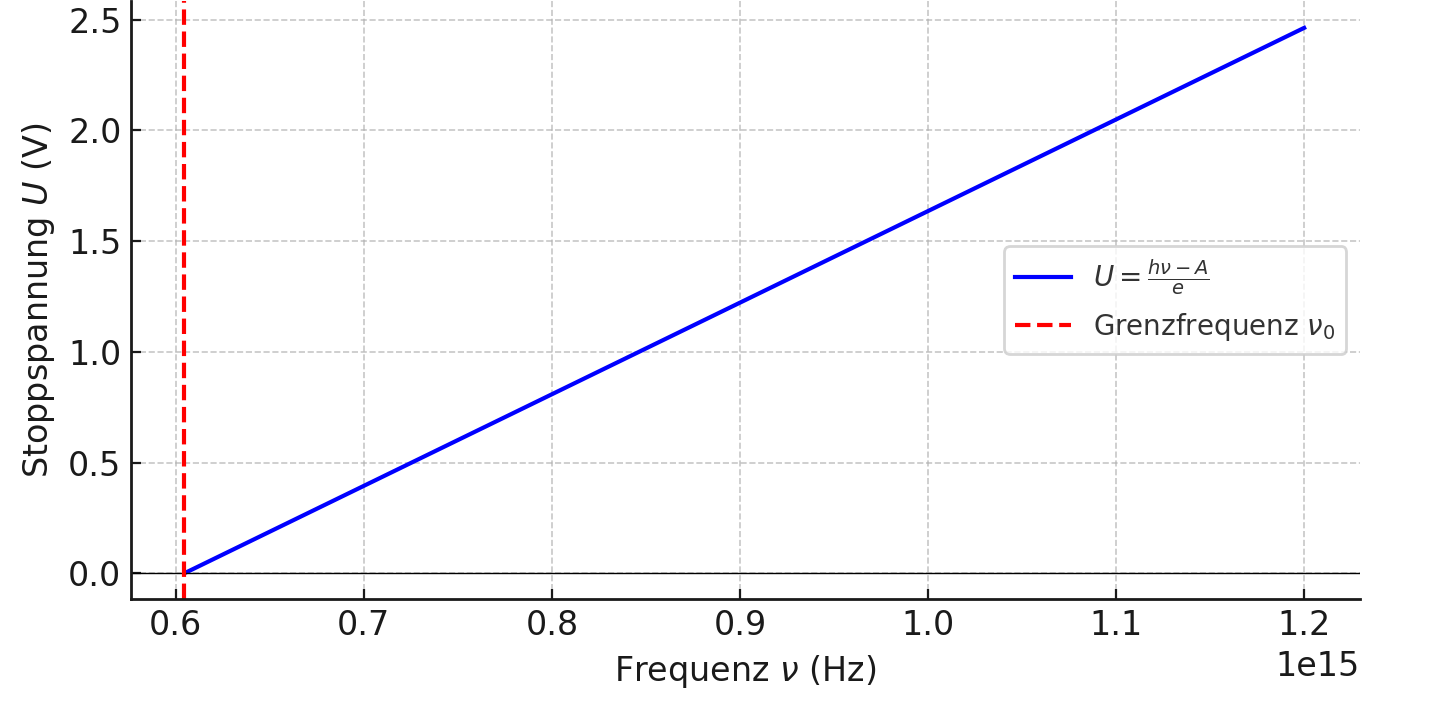
\includegraphics[width=0.65\textwidth]{bilder/photoeffekt.png}
	\caption{lineare Abhängigkeit der Elektronrnernergie}
\end{figure}

\begin{itemize}
	\item Die \textbf{Steigung} der Geraden entspricht \( h/e \)
	\item Der \textbf{x-Achsenabschnitt} \( \nu_0 \) ist die Grenzfrequenz: \( h \nu_0 = A \)\index{Grenzfrequenz}
	\item Für \( \nu < \nu_0 \) tritt keine Emission auf – unabhängig von der Intensität
\end{itemize}

Diese lineare Beziehung wurde von Millikan experimentell mit hoher Genauigkeit bestätigt.\index{Millikan, Robert A.}

\textbf{Dies hat dann zur Folge:}

\begin{quote}
	Die Energie eines Photons hängt allein von der Frequenz ab – nicht von der Lichtintensität.
\end{quote}
\index{Frequenz}\index{Intensität}
\subsubsection{ Vergleich: Wellenmodell vs. Photonenmodell}\index{Wellenmodell}\index{Photonenmodell}\index{Welle-Teilchen-Dualismus@Welle-Teilchen-Dualismus (Kontrast)}

Die Erklärung des Photoeffekts markiert einen tiefgreifenden Paradigmenwechsel in der Physik: von der klassischen Wellenvorstellung des Lichts hin zu einem quantisierten Teilchenbild.\index{Paradigmenwechsel} Um die Tragweite dieses Wechsels zu verdeutlichen, lohnt sich eine direkte Gegenüberstellung beider Modelle.

\vspace{1em}
\begin{table}[H]
	\centering
	\begin{tabular}{|p{4.75cm}|p{4.75cm}|} % vorher 5cm
		\hline
		\textbf{Klassisches Wellenmodell} & \textbf{Photonenmodell (Einstein)} \\
		\hline
		Licht ist eine kontinuierliche Welle im elektromagnetischen Feld & Licht besteht aus einzelnen Quanten (Photonen) mit Energie \( E = h\nu \) \\
		\hline
		Energie wird über die Feldstärke kontinuierlich übertragen & Energie wird stoßartig in diskreten Portionen übertragen \\
		\hline
		Intensität bestimmt die Energieübertragung & Intensität bestimmt nur die \emph{Anzahl} der Photonen, nicht deren Energie \\
		\hline
		Jede Frequenz kann bei genügender Intensität Elektronen lösen & Nur Photonen mit \( h\nu > A \) lösen Elektronen aus \\
		\hline
		Energie wird langsam angesammelt; Zeitverzögerung möglich & Sofortige Emission bei Photontreffer \\
		\hline
	\end{tabular}
	\caption{Vergleich zwischen klassischem Wellenmodell und Photonenmodell beim Photoeffekt}
	\label{tab:vergleich_photoeffekt}
\end{table}
\newpage
\noindent
\vspace{1em}

\begin{tcolorbox}[didaktikbox, title=Didaktische Klarstellung]
	\label{box:didaktischeKlarstellung}
	\small
	Die Intensität des Lichts entscheidet im Wellenmodell über die Stärke der Energieübertragung – im Photonenmodell jedoch nur über die Anzahl der auftreffenden Quanten.\\
	Die Energie eines einzelnen Photons hängt ausschließlich von der Frequenz ab.
\end{tcolorbox}
\vspace{1em}
\index{Intensität}\index{Frequenz}\index{Photon}
\textbf{Typisches Missverständnis:}  
„Helles Licht muss stärkere Elektronen auslösen.“  
$\rightarrow$ \emph{Falsch}, denn bei Licht unterhalb der Grenzfrequenz geschieht – unabhängig von der Helligkeit – gar nichts.\index{Grenzfrequenz}

\textbf{Einordnung:}  
Der Photoeffekt war der erste direkte Nachweis dafür, dass elektromagnetische Strahlung nicht nur Wellencharakter, sondern auch Teilcheneigenschaften besitzt. Diese Dualität wurde später im Konzept des Welle-Teilchen-Dualismus verallgemeinert.\index{Welle-Teilchen-Dualismus}
\subsubsection{Bedeutung für die Physik}\index{Photoeffekt!Bedeutung}\index{Photon}\index{Quantennatur des Lichts@Quantennatur des Lichts}\index{Einstein, Albert}\index{Klassische Elektrodynamik}

Der Photoeffekt war das erste Phänomen, das sich nur durch die Annahme einer diskreten Quantennatur des Lichts erklären ließ. Einsteins Lichtquantenhypothese von 1905 widersprach der klassischen Elektrodynamik und wurde zunächst als spekulativ abgetan. Doch Millikans präzise Bestätigung im Jahr 1916 zwang die Fachwelt, das Bild des Lichts grundlegend zu überdenken.\index{Millikan, Robert A.}

\textbf{Physikalische Konsequenzen:}
\begin{itemize}
	\item Die Energieübertragung des Lichts erfolgt nicht kontinuierlich, sondern in diskreten Quanten – den Photonen.\index{Photon}
	\item Die Energie eines Photons ist proportional zur Frequenz: \( E = h\nu \).\index{Planck-Einstein-Beziehung@$E=h\nu$}\index{Frequenz}
	\item Der Photoeffekt lieferte den ersten direkten experimentellen Nachweis für diese Quantisierung.\index{Photoeffekt!Nachweis}
\end{itemize}

Einstein selbst erhielt 1921 den Nobelpreis – ausdrücklich nicht für die Relativitätstheorie, sondern:\index{Nobelpreis!Einstein 1921}\index{Relativitätstheorie}
\begin{quote}
	„für seine Verdienste um die theoretische Physik, insbesondere für seine Entdeckung des Gesetzes des Photoelektrischen Effekts.“
\end{quote}

Auch Millikan wurde 1923 mit dem Nobelpreis ausgezeichnet – für seine Bestimmung der Elementarladung und seine Arbeiten zum Photoeffekt.\index{Nobelpreis!Millikan 1923}\index{Elementarladung}

\vspace{1em}
\begin{tcolorbox}[hinweisbox, title=Fazit]
	\label{box:fazit der photo}
	\small
	Der Photoeffekt markiert den Anfang des Photonenbegriffs – und damit den Beginn der Quantenphysik.\\
	Er zeigt: Licht besitzt nicht nur Welleneigenschaften, sondern verhält sich unter bestimmten Bedingungen wie ein Teilchen.
\end{tcolorbox}
\index{Quantenphysik}
\vspace{1em}
\textbf{Ausblick:}  
Im nächsten Abschnitt betrachten wir ein weiteres Schlüsselexperiment: die \textbf{Compton-Streuung}. Sie zeigt nicht nur die Energie-, sondern auch die \emph{Impulsübertragung} von Photonen – ein entscheidender Beleg für den Teilchencharakter des Lichts.\index{Compton-Streuung}\index{Impulsübertragung}

\subsection{Die Compton-Streuung}\index{Compton-Streuung}\index{Compton, Arthur H.}\index{Röntgenstrahlung}

\subsubsection{Das Compton-Experiment (1923)}\index{Compton, Arthur H.!Experiment (1923)}

Im Jahr 1923 veröffentlichte der amerikanische Physiker \textbf{Arthur H. Compton} die Ergebnisse eines Streuexperiments mit Röntgenstrahlung, das die Physik revolutionieren sollte. Er ließ hochenergetische Photonen auf nahezu freie Elektronen treffen – etwa in Graphit –, und analysierte die gestreute Strahlung in Abhängigkeit vom Winkel.\index{Elektron}\index{Graphit}

Die zentrale Beobachtung war verblüffend: Das gestreute Licht hatte eine größere Wellenlänge (niedrigere Energie) als das einfallende, und die Wellenlängenverschiebung war systematisch vom Streuwinkel abhängig.\index{Wellenlängenverschiebung}\index{Streuwinkel}

Diese Veränderung ließ sich weder durch klassische Streuung (wie bei Thomson) noch durch Interferenz erklären. Compton interpretierte das Ergebnis als \textbf{elastischen Stoß} zwischen einem Photon und einem Elektron – ganz im Sinne eines Teilchenmodells des Lichts. Damit wurde das Photon nicht nur Träger von Energie, sondern auch von Impuls.\index{Thomson-Streuung}\index{Elastischer Stoß}\index{Photonenimpuls}

\textbf{Physikalisches Prinzip:}
\begin{itemize}
	\item Ein Photon mit Wellenlänge \( \lambda \) trifft auf ein ruhendes Elektron.
	\item Beim Stoß wird das Photon abgelenkt (Streuwinkel \( \theta \)) und gibt dabei Impuls und Energie an das Elektron ab.
	\item Das gestreute Photon besitzt eine neue Wellenlänge \( \lambda' > \lambda \).
\end{itemize}

\textbf{Zentrale Gleichung:}
\[
\Delta \lambda = \lambda' - \lambda = \frac{h}{m_e c}(1 - \cos \theta)
\]\index{Compton-Formel}\index{Compton-Wellenlänge}\index{Elektron!Masse $m_e$}

\vspace{1em}
\begin{figure}[H]
	\begin{center}
		
		
		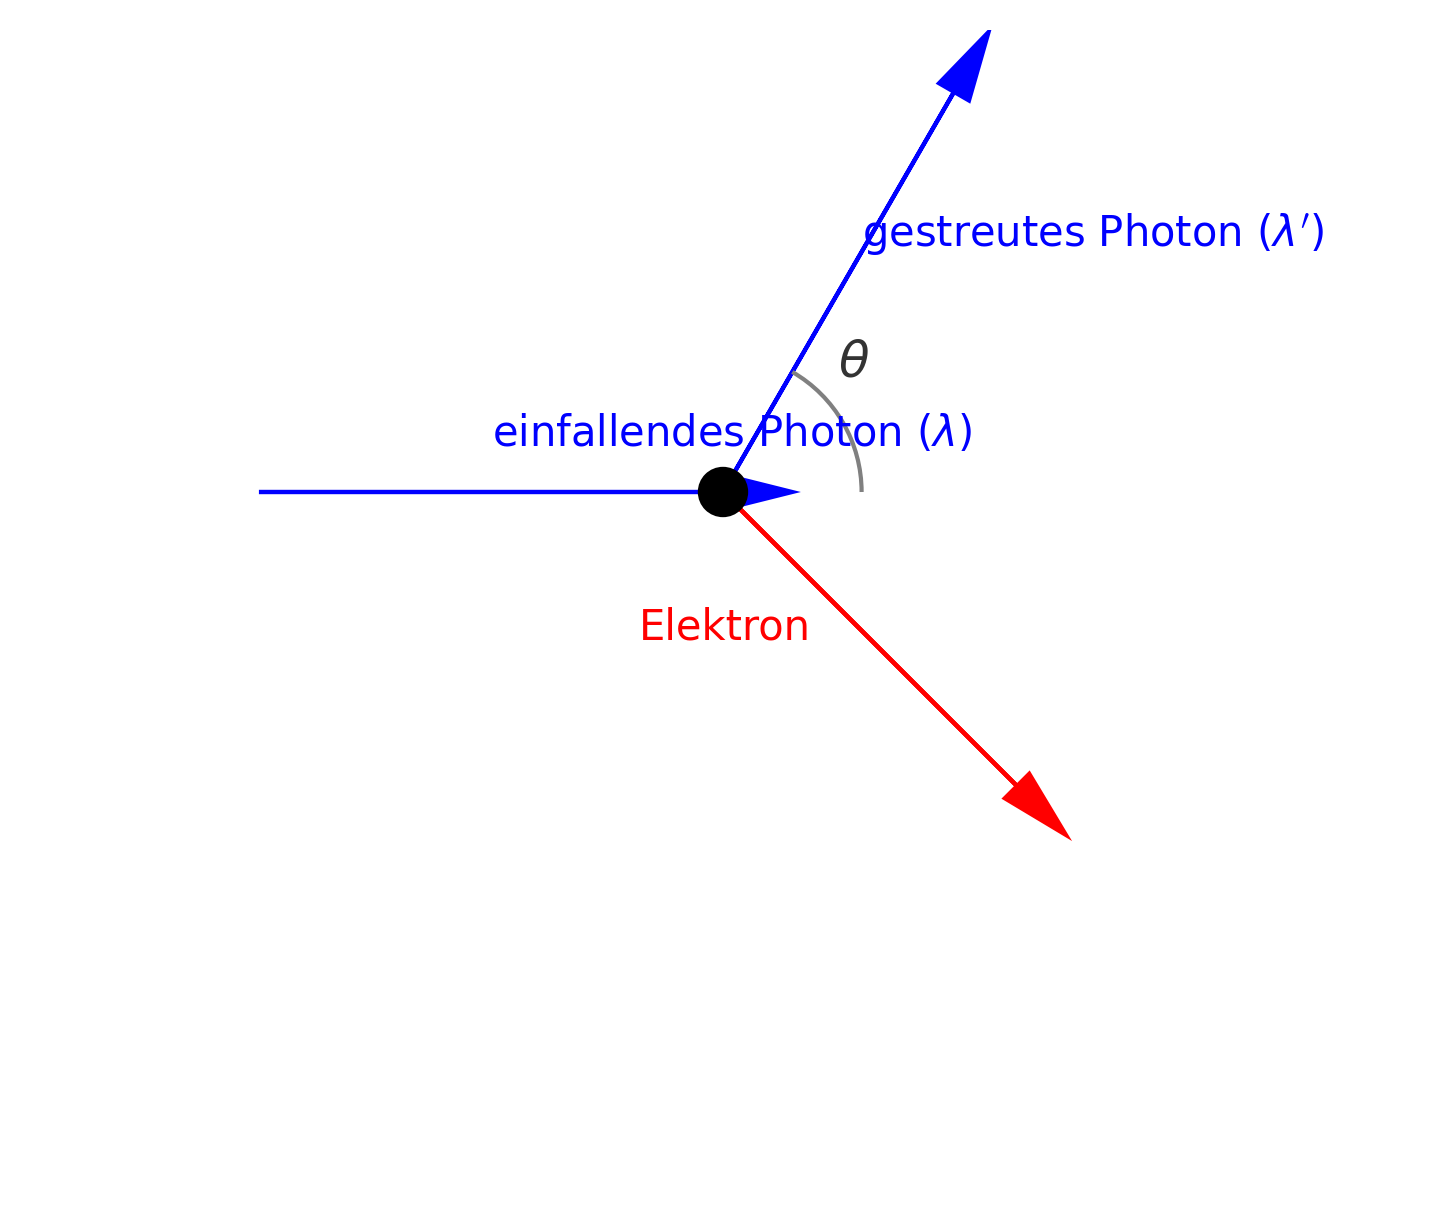
\includegraphics[width=0.6\textwidth]{bilder/compton-schema.png}
	\end{center}
	\caption{Schematische Darstellung der Compton-Streuung: Ein Photon überträgt Impuls auf ein Elektron.}
\end{figure}

\textbf{Bedeutung:}  
Die Compton-Streuung ist der erste experimentelle Beleg dafür, dass Photonen Impuls besitzen – ein entscheidender Schritt zur Anerkennung des Photons als echtes Teilchen. Arthur Compton erhielt dafür 1927 den Nobelpreis für Physik.\index{Photonenimpuls}\index{Nobelpreis!Compton 1927}

\subsubsection{Kompakte Herleitung der Compton-Formel}\index{Compton-Formel!Herleitung}\index{Energieerhaltung}\index{Impulserhaltung}

Die zentrale Beobachtung beim Compton-Effekt ist: Das gestreute Photon hat eine größere Wellenlänge als das einfallende. Diese Verschiebung lässt sich nur erklären, wenn man dem Photon nicht nur Energie \( E = h\nu \), sondern auch Impuls \( p = h/\lambda \) zuschreibt.\index{Planck-Einstein-Beziehung@$E=h\nu$}\index{Photonenimpuls}

\textbf{Grundidee der Herleitung:}
Das Photon trifft auf ein ruhendes Elektron. Beim Stoß wird Energie und Impuls auf das Elektron übertragen. Die Situation ähnelt einem elastischen Stoß zweier Teilchen – mit dem Unterschied, dass eines davon masselos ist.\index{Elastischer Stoß}\index{Masselose Teilchen}
\newpage
\noindent
\textbf{Zentrale Annahmen:}
\begin{itemize}
	\item \textbf{Energieerhaltung:} Die Summe aus Photonenenergie und Elektronenruheenergie bleibt erhalten.
	\item \textbf{Impulserhaltung:} Die Impulsvektoren vor und nach dem Stoß müssen sich vektoriell ausgleichen – in x- und y-Richtung.
	\item \textbf{Photonenimpuls:} Für das Photon gilt \( p = \frac{h}{\lambda} \), für das Elektron relativistische Energie-Impuls-Beziehung.\index{Relativistische Energie-Impuls-Beziehung}
\end{itemize}

Durch Anwendung dieser Erhaltungssätze ergibt sich nach Umformung die \textbf{Compton-Formel}:

\vspace{1em}
\begin{tcolorbox}[mathebox, title=Compton-Formel]
	\label{box:comptonFormel}
	\small
	\[
	\Delta \lambda = \lambda' - \lambda = \frac{h}{m_e c}(1 - \cos \theta)
	\]
\end{tcolorbox}
\vspace{1em}
(Eine ausführlichere Herleitung der Compton-Formel findet sich in Anhang~A, Abschnitt~\ref{anhangA:comptonHerleitung}.) % NEU
\textbf{Physikalische Interpretation:}
\begin{itemize}
	\item Die Wellenlänge des gestreuten Photons ist umso größer, je größer der Streuwinkel \( \theta \) ist.\index{Streuwinkel}
	\item Der Faktor \( \frac{h}{m_e c} \approx 2{,}43 \cdot 10^{-12}\,\mathrm{m} \) wird als \emph{Compton-Wellenlänge} des Elektrons bezeichnet.\index{Compton-Wellenlänge}
	\item Der Effekt zeigt, dass das Photon \emph{Impuls} überträgt – ein klarer Beleg für seinen Teilchencharakter.\index{Photonenimpuls}
\end{itemize}

\vspace{1em}

\subsection{Doppelspaltversuch mit einzelnen Photonen}\index{Doppelspaltversuch}\index{Einzelphoton}\index{Interferenz}\index{Welle-Teilchen-Dualismus}

Ein zentrales Argument für den Wellencharakter des Lichts war seit dem 19. Jahrhundert die Beobachtung von Interferenzmustern – insbesondere im berühmten Doppelspaltversuch. Doch moderne Experimente zeigen: Auch einzelne Photonen, die nacheinander durch den Versuchsaufbau geschickt werden, erzeugen am Schirm ein Interferenzmuster. Dies ist nur erklärbar, wenn man dem Photon auch Wellencharakter zuschreibt.\index{Interferenzmuster}
\newpage
\noindent
\textbf{Experimenteller Aufbau:}
\begin{itemize}
	\item Eine schwache Lichtquelle sendet einzelne Photonen aus – so schwach, dass sich niemals zwei gleichzeitig im Aufbau befinden.\index{Einzelphotonenquelle}
	\item Die Photonen passieren zwei eng beieinanderliegende Spalte (Doppelspalt).\index{Doppelspalt}
	\item Dahinter befindet sich ein lichtempfindlicher Schirm oder Detektor.\index{Detektor}
\end{itemize}

\textbf{Beobachtung:}
\begin{itemize}
	\item Jedes einzelne Photon wird punktuell registriert – wie ein Teilchen.\index{Teilchencharakter des Lichts}
	\item Nach und nach entsteht jedoch ein Interferenzmuster – wie bei einer Welle.\index{Wellencharakter des Lichts}
\end{itemize}

\vspace{1em}
\begin{figure}[H]
	\begin{center}
		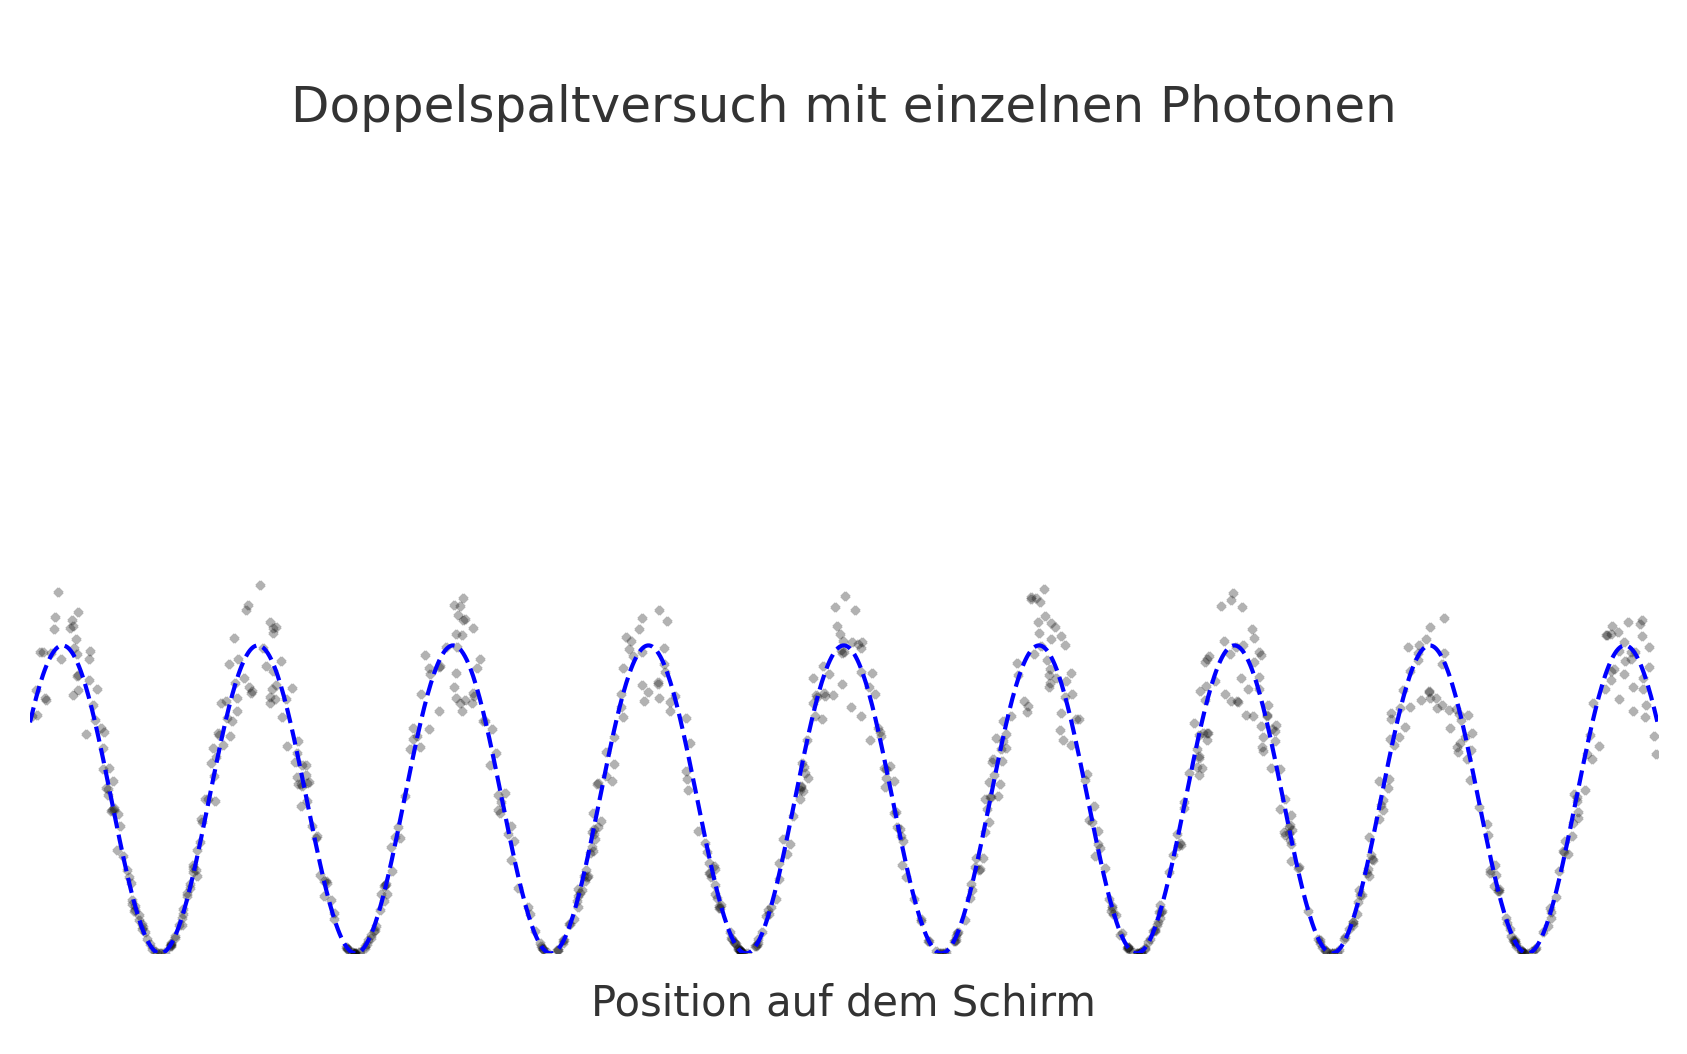
\includegraphics[width=0.65\textwidth]{bilder/doppelspalt-photonen.png}
	\end{center}
	\caption{Doppelspaltversuch mit einzelnen Photonen: Teilchendetektion mit Wellenmuster.}
\end{figure}

\begin{tcolorbox}[physikbox, title=Was die Photonengrafik zeigen soll]
	\label{box:was die photonengrafik}
	\small
	\begin{itemize}
		\item Die Punkte stehen für einzelne Photondetektionen – der Teilchenaspekt des Lichts.
		\item Mit der Zeit entsteht ein Muster, das typisch für Welleninterferenz ist – wie bei Wasserwellen.
		\item Die gestrichelte Linie zeigt nur die statistische Häufigkeit der Auftrefforte – sie ist kein Lichtstrahl und keine reale Welle.
	\end{itemize}
\end{tcolorbox}
\vspace{1em}
(Das mathematische Formalisieren des Doppelspaltversuchs mit einzelnen Photonen und die Superpositionsdarstellung finden sich in Anhang~A, Abschnitt~\ref{anhangA:doppelspalt}.) % NEU
\textbf{Interpretation:}  
Das Photon interferiert offenbar mit sich selbst – es „geht gleichzeitig durch beide Spalte“. Erst beim Nachweis am Schirm kollabiert der Zustand in ein einzelnes Ereignis. Dieses Verhalten lässt sich nur im Rahmen der Quantenmechanik verstehen: Das Photon ist weder klassische Welle noch klassisches Teilchen – es zeigt beides, abhängig vom Experiment.\index{Selbstinterferenz}\index{Quantenmechanik}\index{Zustandskollaps@Kollaps der Wellenfunktion}

\vspace{1em}
\begin{tcolorbox}[hypobox, title=Schlüsselidee]
	\label{box:schlüsselidee}
	\small
	Der Doppelspaltversuch mit einzelnen Photonen zeigt: Die Quantennatur des Lichts beinhaltet sowohl Wellen- als auch Teilcheneigenschaften. Das Interferenzmuster entsteht, obwohl niemals zwei Photonen gleichzeitig im System sind.
\end{tcolorbox}
\vspace{1em}
\begin{tcolorbox}[didaktikbox, title=Wellen-als auch Teilcheneigenschaften]
	\label{box:wellen}
	\small
	Das Interferenzmuster verschwindet sofort, wenn man versucht, den Weg des Photons durch einen der Spalte zu bestimmen. Die Möglichkeit zur Interferenz ist an die \emph{Unkenntnis des Weges} gebunden – ein Grundprinzip der Quantenphysik.
\end{tcolorbox}
\index{Welcher-Weg-Information}

\subsubsection*{Zusammenfassung}\index{Doppelspaltversuch!Zusammenfassung}\index{Superposition}

\phantomsection
\begin{tcolorbox}[didaktikbox, title=Fazit: Ein scheinbar paradoxes Verhalten]
	\label{box:Fazit ein scheinbarer}
	\small
	Selbst wenn Photonen einzeln – also nacheinander – durch den Doppelspalt geschickt werden, entsteht mit der Zeit ein Interferenzmuster.
	
	Das wirft eine tiefgreifende Frage auf: Woher „weiß“ ein einzelnes Photon, dass es Teil eines Musters ist?
	
	Im klassischen Sinne müsste es eine Art Kommunikation zwischen den Photonen geben – doch dem ist nicht so. Jedes Photon scheint mit sich selbst zu interferieren. Die Quantenmechanik erklärt dies durch die \textbf{Überlagerung aller möglichen Wege}: Das Photon ist nicht durch den einen oder den anderen Spalt gegangen – sondern durch beide, solange der Weg nicht gemessen wird.
	
	Diese Vorstellung widerspricht unserer Alltagserfahrung – ist aber experimentell zweifelsfrei belegt. Der Doppelspaltversuch ist damit ein Schlüsselergebnis der Quantenphysik.
	
	Der Doppelspaltversuch mit einzelnen Photonen stellt unser klassisches Denken infrage:  
	Wie kann ein einzelnes Photon zum Aufbau eines Interferenzmusters beitragen, obwohl kein zweites Photon gleichzeitig im Versuchsaufbau ist?
	
	Offenbar scheint jedes Photon mit sich selbst zu interferieren. In der Sprache der Quantenmechanik bedeutet das: Solange kein Messgerät den Weg bestimmt, überlagern sich alle möglichen Wege gleichzeitig – auch „durch beide Spalte zugleich“.
	
	Diese Superposition kollabiert erst bei der Detektion zu einem einzelnen Punkt. Das Interferenzmuster entsteht nicht durch Wechselwirkung der Photonen untereinander, sondern durch die \emph{Statistik vieler Einzelmessungen} – und durch die quantenmechanische Struktur des Zustandsraums.
	
	Was nach „Kommunikation“ aussieht, ist in Wahrheit ein Ausdruck der Nichtklassizität der Quantenwelt.
\end{tcolorbox}

\subsection{Antibunching: Der Nachweis einzelner \newline Photonen}\index{Antibunching}\index{Einzelphoton}\index{Einzelphotonenquelle}\index{Strahlteiler}\index{Detektor}

Ein besonders überzeugender experimenteller Beweis für die Existenz einzelner Photonen liefert das Phänomen des \textbf{Antibunching}. Dabei wird eine Lichtquelle verwendet, die nur jeweils ein Photon auf einmal abstrahlen kann – z.\,B. ein fluoreszierendes Atom oder Quantenpunkt.\index{Quantenpunkt}\index{Fluoreszenz}

In einem Aufbau mit Strahlteiler und zwei Detektoren zeigt sich: Es \emph{kommt niemals vor}, dass beide Detektoren gleichzeitig ein Signal registrieren. Das bedeutet: Es gibt kein „halbes“ Photon – sondern immer genau eines, das entweder hier oder dort ankommt.\\
\textbf{Warum widerspricht das der klassischen Wellenvorstellung?} \\
In der klassischen Theorie ist Licht eine kontinuierliche elektromagnetische Welle. Trifft eine solche Welle auf einen Strahlteiler, so wird sie \emph{aufgeteilt}: Ein Teil geht nach links, der andere nach rechts. Damit müssten – zumindest bei starker Intensität – auch beide Detektoren gleichzeitig ein Signal registrieren.\index{Klassische Elektrodynamik}\index{Wellenmodell}

Beim Antibunching hingegen zeigt sich: \emph{Nie} werden beide Detektoren gleichzeitig ausgelöst. Das bedeutet, dass das Licht nicht aufgeteilt ankommt, sondern in \textbf{unteilbaren Energiepaketen} – einzelnen Photonen. Genau das widerspricht der Vorstellung einer klassischen Welle.\index{Photon!Unteilbarkeit}

\vspace{1em}
\begin{tcolorbox}[physikbox, title=Was Antibunching zeigt]
	\label{box:wasAntibunching}
	\small
	Licht kann nicht gleichzeitig in zwei Richtungen aufgeteilt werden, wenn es aus einzelnen Photonen besteht.\\
	Dies widerspricht jeder klassischen Wellenvorstellung – aber entspricht genau dem Verhalten unteilbarer Lichtquanten.
\end{tcolorbox}
\vspace{1em}
(Eine mathematische Beschreibung der zweiten Ordnungs-Korrelations\-funktion \( g^{(2)}(0) \) findet sich in Anhang~A, Abschnitt~\ref{anhangA:antibunching}.) % NEU
\subsection{Hong-Ou-Mandel-Effekt: \newline Interferenz zweier Photonen}\index{Hong-Ou-Mandel-Effekt}\index{Ununterscheidbarkeit (Photonen)@Ununterscheidbarkeit von Photonen}\index{Wahrscheinlichkeitsamplitude}\index{Strahlteiler}

Ein weiteres eindrucksvolles Experiment ist der \textbf{Hong-Ou-Mandel-Effekt}. Zwei identische Photonen werden aus zwei entgegengesetzten Richtungen auf einen halbdurchlässigen Spiegel (Strahlteiler) gelenkt.
\begin{figure}[H]
	\begin{center}
		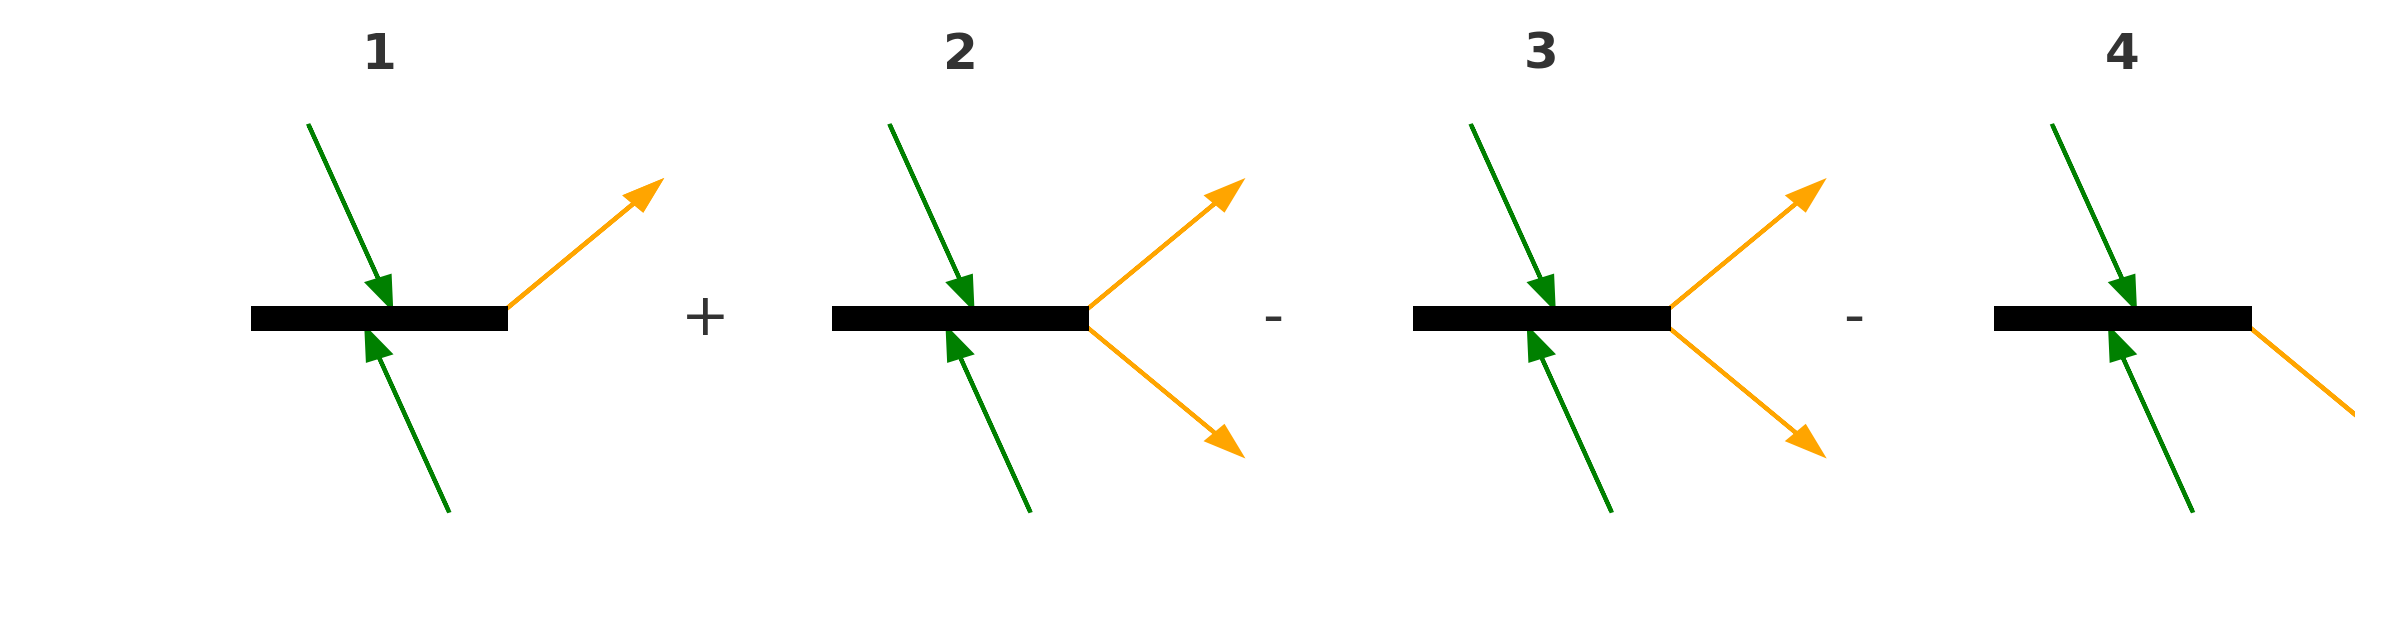
\includegraphics[width=0.95\textwidth]{bilder/hom_interferenzpfade_korrigiert.png}
		
	\end{center}
	\caption{Vier mögliche Pfade zweier Photonen am Strahlteiler.\\
		Die mittleren Fälle führen zu Koinzidenz – löschen sich aber durch Interferenz aus}
\end{figure}

\begin{tcolorbox}[hinweisbox, title=Was diese Darstellung zeigt]
	\label{box:was diese Darstellun}
	\small
	Das Diagramm zeigt die vier möglichen Pfade, die zwei identische Photonen beim Auftreffen auf einen Strahlteiler nehmen können.\\
	In den Fällen 1 und 4 verlassen beide Photonen gemeinsam denselben Ausgang – wie es experimentell beobachtet wird.
	
	Die Pfade 2 und 3 würden dazu führen, dass die Photonen an unterschiedlichen Detektoren ankommen (Koinzidenz). Doch genau diese Fälle löschen sich durch destruktive Interferenz aus – aufgrund der Ununterscheidbarkeit der Photonen und der quantenmechanischen Überlagerung ihrer Amplituden.
	
	Das Ergebnis: Bei perfekter Überlappung werden niemals gleichzeitig beide Detektoren ausgelöst – ein klarer Hinweis auf die Quantennatur des Lichts.
\end{tcolorbox}

Nach klassischer Erwartung müsste jedes Photon mit 50\,\% Wahrscheinlichkeit reflektiert oder transmittiert werden. Doch in der Quantenrealität passiert etwas anderes: Beide Photonen verlassen immer denselben Ausgang – nie gegensätzlich.\index{Reflexion}\index{Transmission}

Dieses Phänomen entsteht durch die Interferenz der \emph{Wahrscheinlichkeitsamplituden} beider Prozesse. Es zeigt: Photonen sind ununterscheidbar und können auf Quantenebene interferieren – nicht als Felder, sondern als Teilchen mit Wellennatur.\index{Interferenz}\index{Ununterscheidbarkeit (Photonen)@Ununterscheidbarkeit von Photonen}

\vspace{1em}
\begin{tcolorbox}[physikbox, title=Was der HOM-Effekt zeigt]
	\label{box:HOM-Effekt}
	\small
	Zwei Photonen können „verhindern“, dass sie unterschiedliche Wege nehmen – durch Interferenz ihrer Quantenzustände.\\
	Dies ist nur erklärbar, wenn man Photonen als ununterscheidbare Quantenteilchen betrachtet.
\end{tcolorbox}

\subsection{Fazit}\index{Photoeffekt}\index{Compton-Streuung}\index{Doppelspaltversuch}\index{Antibunching}\index{Hong-Ou-Mandel-Effekt}\index{Welle-Teilchen-Dualismus}

\begin{tcolorbox}[hinweisbox, title=Was die Experimente über Licht zeigen]
	\label{box:was die Experimente}
	\small
	Die vier in diesem Kapitel behandelten Experimente – Photoeffekt, Compton-Streuung, Doppelspalt mit einzelnen Photonen und moderne Quantenexperimente wie Antibunching und Hong-Ou-Mandel-Effekt – zeigen eindrucksvoll, dass Licht nicht allein durch klassische Modelle erklärbar ist.
	
	\begin{itemize}
		\item Der \textbf{Photoeffekt} zeigt: Licht überträgt \emph{Energie} in diskreten Portionen (Photonen).
		\item Die \textbf{Compton-Streuung} zeigt: Photonen besitzen auch \emph{Impuls} – wie Teilchen.
		\item Der \textbf{Doppelspaltversuch} zeigt: Photonen zeigen \emph{Wellenmuster} in ihrer Verteilung – selbst wenn sie einzeln auftreten.
		\item \textbf{Antibunching} und der \textbf{Hong-Ou-Mandel-Effekt} zeigen: Photonen sind \emph{nicht teilbar}, \emph{nicht klassisch unterscheidbar} und unterliegen den Regeln der Quantenmechanik.
	\end{itemize}
	(Eine detailliertere Herleitung der quantenmechanischen Interferenz am Strahlteiler beim HOM-Effekt findet sich in Anhang~A, Abschnitt~\ref{anhangA:HOM}.) % NEU
	Diese Experimente beweisen gemeinsam: Licht ist kein Entweder-Oder aus Welle und Teilchen – es ist beides zugleich, abhängig vom Experiment. Der Photonenbegriff ist damit nicht nur ein Rechenkonzept – sondern physikalisch real.
\end{tcolorbox}

	\chapter{Das Photon in der Quantenelektrodynamik (QED)}\index{Photon}\index{Quantenelektrodynamik (QED)}
\setcounter{section}{5}
\setcounter{subsection}{0}
\setcounter{subsubsection}{1}
\setcounter{secnumdepth}{3}
\setlength{\parindent}{0pt}
% Boxen-Stile definieren
\tcbset{physikbox/.style={colback=blue!5!white, colframe=blue!75!black, fonttitle=\bfseries}}
\tcbset{mathebox/.style={colback=green!5!white, colframe=green!50!black, fonttitle=\bfseries}}
\tcbset{didaktikbox/.style={colback=yellow!5!white, colframe=yellow!50!black, fonttitle=\bfseries}}
\tcbset{hypobox/.style={colback=orange!5!white, colframe=orange!75!black, fonttitle=\bfseries}}
\tcbset{hinweisbox/.style={colback=gray!10!white, colframe=black!40!black, fonttitle=\bfseries}}
\tcbset{warnbox/.style={colback=red!10!white, colframe=red!40!black, fonttitle=\bfseries}}

\subsection{Vom Photon zur Quantenelektrodynamik}\index{Quantenelektrodynamik (QED)!Einführung}\index{Photoeffekt}\index{Compton-Streuung}\index{Einstein, Albert}\index{Maxwell, James Clerk}\index{Austauschteilchen}
% Historischer und theoretischer Übergang: von der klassischen Elektrodynamik über die Quantenoptik zur QED

Die Geschichte des Photons beginnt mit einem Paradoxon: Das Licht, das man seit dem 19. Jahrhundert als elektromagnetische Welle verstand, zeigte bei bestimmten Experimenten ein Verhalten, das nur mit einem Teilchenbild erklärbar war – insbesondere beim Photoeffekt und der Compton-Streuung.\index{Wellenmodell}\index{Teilchenmodell}
Diese Experimente führten zur Einführung des Begriffs des \emph{Lichtquants} durch Einstein im Jahr 1905.\index{Lichtquant}
Doch obwohl sich das Photonenmodell experimentell bewährte, blieb es über Jahrzehnte umstritten.\index{Photonenmodell}

Ein vollständiges theoretisches Verständnis der Lichtmaterie-Wechsel\-wirkung gelang erst mit der Entwicklung der \textbf{Quantenelektrodynamik} (QED).\index{Licht-Materie-Wechsel wirkung}\index{Relativitätstheorie!Spezielle}\index{Quantenmechanik}
Sie verbindet die klassische Feldtheorie Maxwells mit den Prinzipien der Quantenmechanik und der speziellen Relativitätstheorie.
In der QED ist das Photon das Austauschteilchen der elektromagnetischen Wechselwirkung – ein masseloses, Spin-1-Trägerteilchen, das nicht nur reale, sondern auch virtuelle Zustände annehmen kann.\index{Spin}\index{Masselosigkeit}\index{Virtuelle Photonen}
(Eine kompakte Einführung in den Feldformalismus der QED und das Potential \(A^\mu\) findet sich in Anhang~A, Abschnitt~\ref{anhangA:feldformalismus}.)

\vspace{1em}
\begin{tcolorbox}[physikbox, title=Was ist Quantenelektrodynamik?]
	\label{box:was ist quantenelektro}
	\small
	Die Quantenelektrodynamik beschreibt, wie geladene Teilchen (z.\,B. Elektronen) Photonen austauschen und dadurch elektromagnetisch miteinander wechselwirken.\\
	Die Theorie basiert auf quantisierten Feldern, Feynman-Diagrammen und einem lokalen Eichprinzip. Sie ist die präziseste physikalische Theorie, die bisher experimentell getestet wurde.
\end{tcolorbox}
\vspace{1em}
Der Übergang vom klassischen zum quantenfeldtheoretischen Verständnis war jedoch alles andere als geradlinig. Anfangs betrachtete man Photonen als diskrete Pakete klassischer Wellenenergie – ein Kompromiss zwischen Teilchen- und Wellenbild.\index{Quantenfeldtheorie}\index{Wellenenergie}
Erst in den 1940er-Jahren, mit der Arbeit von Dirac, Feynman, Schwinger und Tomonaga, entstand eine konsistente Theorie, die das Photon als Quant des elektromagnetischen Feldes mathematisch beschreibt.\index{Dirac, Paul A. M.}\index{Feynman, Richard P.}\index{Schwinger, Julian}\index{Tomonaga, Sin-Itiro}\index{Quantisiertes Feld}

\textbf{Was sich mit QED ändert:}
\begin{itemize}
	\item Photonen werden nicht mehr als Lichtstrahlen gedacht, sondern als Anregungen eines quantisierten Feldes.\index{Anregung (Feld)}\index{Lichtstrahl}
	\item Die Wechselwirkung erfolgt nicht kontinuierlich, sondern in diskreten Prozessen (Vertices).\index{Wechselwirkung!Vertex}
	\item Auch virtuelle Photonen – nicht beobachtbar, aber mathematisch erforderlich – spielen eine zentrale Rolle.\index{Virtuelle Photonen}
\end{itemize}
(Zum Übergang vom klassischen Feld zur Quantisierung und zu Feynman-Diagrammen vgl. Anhang~A, Abschnitt~\ref{anhangA:feld_zu_qed}.)

Dieses Kapitel führt in die Eigenschaften des Photons im Rahmen der QED ein, beginnend mit seinem Vektorcharakter, gefolgt von seiner Rolle als Austauschteilchen in Feynman-Diagrammen, bis hin zu experimentellen Bestätigungen mit höchster Präzision.\index{Feynman-Diagramme}

\subsection{Der Vektorcharakter des Photons in der QED}\index{Photon!Vektorcharakter}\index{Polarisation!Transversal}\index{Spin}

Die transversale Polarisation des Photons und seine Eigenschaft als Spin\mbox{-}1\mbox{-}Teilchen wurden bereits in Abschnitt~3.6 beschrieben.\index{Helizität}
In der Quantenelektrodynamik ergibt sich diese Struktur jedoch nicht nur aus experimenteller Beobachtung oder klassischen Gleichungen, sondern aus dem zugrunde liegenden \emph{Feldformalismus} und der \emph{Eichsymmetrie} der Theorie.\index{Feldformalismus}\index{Eichsymmetrie}
(Eine formale Darstellung der Helizität des Photons findet sich zusätzlich in Anhang~A, Abschnitt~\ref{anhangA:helizitaet}; zur Polarisation in Jones-/Dirac-Notation siehe \ref{anhangA:polarisation}.)

\vspace{1em}
\begin{tcolorbox}[physikbox, title=Was ist der Feldformalismus?]
	\label{box:was ist Feldformalismus}
	\small
	In der QED sind Photonen keine „Teilchen mit Bahn“, sondern quantisierte Anregungen eines Feldes: des elektromagnetischen Potentials \( A^\mu(x) \). So wie eine Wasserwelle ein lokaler Ausschlag der Wasseroberfläche ist, ist ein Photon eine diskrete Schwingung des Feldes – beschrieben durch Quantenmechanik und Relativität zugleich.
\end{tcolorbox}
\vspace{1em}
\index{Vektorpotential $A^\mu$}
(Eine kurze Ableitung der Lorentz-kovarianten Form des Viererpotentials \(A^\mu\) steht in Anhang~A, Abschnitt~\ref{anhangA:viererpotential}.)

Der zentrale mathematische Ausgangspunkt ist die sogenannte \emph{Lagrangedichte} \( \mathcal{L} \), aus der die Bewegungsgleichungen des Feldes abgeleitet werden.\index{Lagrangedichte}\index{Bewegungsgleichungen}
Für das elektromagnetische Feld lautet sie:

\[
\mathcal{L}_{\text{EM}} = -\frac{1}{4} F_{\mu\nu} F^{\mu\nu}
\quad \text{mit} \quad F_{\mu\nu} = \partial_\mu A_\nu - \partial_\nu A_\mu
\]\index{Feldstärketensor $F_{\mu\nu}$}
(Herleitung von Feldstärketensor und EM-Lagrangedichte: Anhang~A, Abschnitte~\ref{anhangA:feldstaerketensor} und \ref{anhangA:lagrange_em}; zur Energie-Impuls-Relation vgl. \ref{anhangA:energie_impuls}.)

Diese Lagrangedichte führt – über das Prinzip der kleinsten Wirkung – auf die Maxwellschen Gleichungen in ihrer relativistischen Form.\index{Prinzip der kleinsten Wirkung}\index{Maxwellsche Gleichungen}
Sie ist invariant unter sogenannten \textbf{Eichtransformationen}:

\[
A^\mu(x) \rightarrow A^\mu(x) + \partial^\mu \Lambda(x)
\]\index{Eichtransformation}
(Zur lokalen \(U(1)\)-Eichsymmetrie, Eichfixierung und \newline Lorenz-Bedingung siehe Anhang~A, Abschnitt~\ref{anhangA:eichsymmetrie}.)
\vspace{1em}
\begin{tcolorbox}[physikbox, title=Was bedeutet Eichsymmetrie?]
	\label{box:was bedeutet Eichsy}
	\small
	Eichsymmetrie bedeutet, dass man das elektromagnetische Potential \( A^\mu(x) \) lokal verändern kann, ohne dass sich messbare Größen wie das elektrische Feld ändern. Diese Freiheit ist kein Rechenkunststück, sondern strukturbildend: Sie bestimmt, welche Terme erlaubt sind – und welche nicht.
\end{tcolorbox}

\textbf{Warum ist das Photon masselos?}\index{Masselosigkeit}
Ein Masseterm der Form \( \frac{1}{2} m^2 A_\mu A^\mu \) wäre unter dieser Transformation \emph{nicht invariant}. Die Forderung nach Eichsymmetrie verbietet ihn – das Photon muss masselos sein.\index{Masseterm}\index{Eichinvarianz}
(Formale Argumentation via Proca-Lagrange­dichte und gebrochene Eichinvarianz: Anhang~A, Abschnitt~\ref{anhangA:masselosigkeit_proca}.)

\textbf{Warum ist das Photon transversal?}\index{Transversalität}
Ein Vektorfeld hat vier Komponenten, aber nicht alle sind physikalisch unabhängig. Die Eichfreiheit und die Lorentz-Invarianz erlauben es, nicht-physikalische Moden zu eliminieren. Am Ende bleiben genau zwei zulässige Polarisationszustände: die transversalen mit Helizität \( +1 \) und \( -1 \).\index{Lorentz-Invarianz}\index{Polarisationszustände}
(Reduktion der Freiheitsgrade, Lorenz-Bedingung und Spur/Projektor-Methode: Anhang~A, Abschnitt~\ref{anhangA:transversalitaet}; vgl. auch \ref{anhangA:helizitaet}.)

\vspace{1em}
\begin{tcolorbox}[physikbox, title=Folgen der Eichsymmetrie]
	\label{box:folgen der Eichsy}
	\small
	Die Eichsymmetrie der QED erklärt zwei grundlegende Eigenschaften des Photons:
	
	\begin{itemize}
		\item \textbf{Masselosigkeit:} Ein Masseterm wäre nicht eichinvariant – daher ist das Photon zwingend masselos.
		\item \textbf{Transversalität:} Die Symmetrie erlaubt nur zwei Polarisationsmoden – beide senkrecht zur Ausbreitungsrichtung.
	\end{itemize}
\end{tcolorbox}

\textbf{Virtuelle Photonen – eine Ausnahme}\index{Virtuelle Photonen}
Während reale Photonen ausschließlich transversale Zustände besitzen, können sogenannte \emph{virtuelle Photonen} – die in inneren Linien von Feynman-Diagrammen auftreten – auch longitudinale oder skalare Komponenten enthalten.\index{Longitudinale Mode}\index{Skalare Mode}
Diese sind jedoch nicht beobachtbar und verschwinden bei physikalischen Vorhersagen (z.\,B. in der Streuamplitude) vollständig.\index{Streuamplitude}
(Longitudinale/skalarer Anteile in Propagatoren und ihre Auslöschung in Observablen: Anhang~A, Abschnitt~\ref{anhangA:virtuelle_moden}.)

\textbf{Fazit:}\index{Eichsymmetrie!Folgen}
In der QED ergibt sich die Struktur des Photons nicht durch Zusatzannahmen, sondern aus dem symmetrischen Aufbau der Theorie selbst. Die Eichsymmetrie ersetzt Intuition – und erzeugt Ordnung.

%index Anhang
\subsection{Virtuelle Photonen und Feynman-Diagramme}\index{Virtuelle Photonen}\index{Feynman-Diagramme}

\subsubsection{Was sind virtuelle Teilchen?}\index{Virtuelle Teilchen}
\addcontentsline{toc}{subsubsection}{5.3.1 Was sind virtuelle Teilchen?}

Virtuelle Teilchen – insbesondere virtuelle Photonen – sind zentrale Rechenelemente in der Quantenfeldtheorie.\index{Quantenfeldtheorie}
Sie unterscheiden sich grundlegend von realen Teilchen, wie sie in einem Detektor nachgewiesen werden können.\index{Reale Teilchen}\index{Detektor}
Ihre Existenz ist \textbf{mathematischer Natur} – und dennoch zeigen sich ihre Wirkungen in realen Experimenten.\index{Mathematisches Objekt}

\subsubsection*{Unterschied: reale  oder virtuelle Teilchen}\index{On-shell}\index{Off-shell}
\phantomsection
\begin{table}[H]
	\centering
	\scriptsize 

{\small
	\begin{center}
		\renewcommand{\arraystretch}{1.3}
		\begin{tabular}{|p{3cm}|p{3.0cm}|p{3.0cm}|}
			\hline
			\textbf{Eigenschaft} & \textbf{Reale Photonen} & \textbf{Virtuelle Photonen} \\
			\hline
			Beobachtbar im Detektor & Ja (z.\,B. Lichtquant im Photoeffekt) & Nein \\
			\hline
			Energie-Impuls-Beziehung & $E = pc$ (on-shell) & $E^2 \ne p^2 c^2$ (off-shell) \\
			\hline
			Lebensdauer & Beliebig lang (bei stabilen Teilchen) & Extrem kurz (durch Unschärferelation) \\
			\hline
			Physikalische Existenz & Ja & Nur als Rechenelement in Diagrammen \\
			\hline
		\end{tabular}
	\end{center}
}
\end{table}
\vspace{1em}

% Mathebox: On-shell-Bedingung
\begin{tcolorbox}[hinweisbox, title=On-shell-Bedingung]
	\label{box:On-shell-Bedingung}
	Ein Teilchen ist \textbf{on-shell}, wenn es die relativistische Energie-Impuls-Beziehung erfüllt:
	\[
	E^2 = p^2 c^2 + m^2 c^4
	\]
	Für masselose Teilchen (z.\,B. Photonen) reduziert sich dies auf:
	\[
	E = pc
	\]
	Off-shell-Zustände treten bei virtuellen Teilchen auf, die nur in Zwischenrechnungen vorkommen.
\end{tcolorbox}
\index{Energie-Impuls-Beziehung}\index{Relativistische Kinematik}

\subsubsection*{Zeit-Energie-Unschärfe}\index{Unschärferelation!Zeit-Energie}
\phantomsection
Nach der Heisenbergschen Unschärferelation gilt:
\[
\Delta E \cdot \Delta t \gtrsim \hbar
\]\index{Heisenberg, Werner}\index{$\hbar$}
Für sehr kurze Zeiten $\Delta t$ ist es also möglich, kurzfristig gegen die Energieerhaltung zu „verstoßen“ – z.\,B. durch das Auftreten eines virtuellen Photons mit scheinbar „falscher“ Energie.\index{Energieerhaltung}
Dieser Effekt ist kein Regelbruch, sondern eine Konsequenz der Quantenmechanik.\index{Quantenmechanik}

\subsubsection*{Interpretation}\index{Zwischenzustand}
\phantomsection

Virtuelle Teilchen treten in \textbf{Zwischenzuständen} auf – etwa wenn ein Elektron kurz ein Photon abstrahlt, das sofort wieder absorbiert wird.\index{Elektron}\index{Absorption}\index{Emission}
Diese Prozesse finden in \textbf{Feynman-Diagrammen} ihren Ausdruck. Die virtuellen Teilchen sind dabei die \textbf{inneren Linien} des Diagramms.\index{Innere Linien (Diagramme)}

\vspace{1em}

% Physikbox: Virtuelle Teilchen

\vspace{1em}
\begin{tcolorbox}[physikbox, title=Virtuelle Teilchen im Quantenvakuum, label=box:virtuelle-teilchen]
	\label{box:virtuelle-teilchen}
	Virtuelle Teilchen entstehen als Zwischenzustände bei quantenmechanischen Wechselwirkungen. Sie erfüllen nicht die klassische Energie-Impuls-Beziehung (sind \emph{off-shell}) und können nicht direkt beobachtet werden.
	
	Trotzdem zeigen sich ihre Effekte in präzisesten Experimenten – etwa beim \textbf{Lamb-Shift} im Wasserstoffspektrum oder bei der \textbf{Anomalie des $g$-Faktors} des Elektrons.
\end{tcolorbox}
\index{Quantenvakuum}\index{Lamb-Shift}\index{g-Faktor!Anomalie}\index{Wasserstoffspektrum}

\vspace{1em}
\begin{tcolorbox}[hinweisbox, title=Indirekte Nachweise virtueller Photonen]
	\label{box:Nachweis virtueller Photonen}
	\small
	\begin{itemize}
		\item \textbf{Lamb-Shift:} In hochpräzisen Spektren des Wasserstoffatoms zeigt sich eine feine Verschiebung der Energieniveaus, die nur mit quantenfeldtheoretischen Korrekturen erklärt werden kann – insbesondere durch den Einfluss virtueller Photonen auf das Elektron.
		\item \textbf{$g$-Faktor-Anomalie:} Das Elektron besitzt ein magnetisches Moment, das geringfügig vom klassischen Wert $g = 2$ abweicht. Diese Abweichung entsteht durch Schleifenprozesse in Feynman-Diagrammen – mit virtuellen Photonen als Vermittlern.
	\end{itemize}
\end{tcolorbox}
\index{Schleifenprozesse}\index{Magnetisches Moment}\index{Elektron}

\vspace{1em}
% Didaktikbox: Denkfehler vermeiden
\begin{tcolorbox}[didaktikbox, title=Virtuell heißt nicht: weniger real?, label=box:virtuell-denkfehler]
	\label{box:virtuell-denkfehler}
	Der Begriff \glqq virtuell\grqq{} kann leicht in die Irre führen. Virtuelle Teilchen sind \textbf{nicht einfach „unreale“ Teilchen} – sie sind präzise definierte mathematische Objekte in der Quantenfeldtheorie.
	
	Sie folgen eigenen Regeln und tragen wesentlich zum richtigen Ergebnis bei – gerade weil sie \emph{nicht} die Bedingungen realer Teilchen erfüllen.
\end{tcolorbox}


\vspace{1em}

\subsubsection*{Übergang}\index{Coulomb-Kraft}\index{Streuung}
\phantomsection

Im nächsten Abschnitt betrachten wir, wie genau diese virtuellen Photonen in der Quantenfeldtheorie die elektromagnetische Wechselwirkung vermitteln – von der klassischen Coulomb-Kraft bis zu Streuprozessen.
\subsubsection{Virtuelle Photonen als Austauschteilchen}\index{Virtuelle Photonen!Austauschteilchen}\index{Austauschteilchen}\index{Wechselwirkung!elektromagnetisch}

In der klassischen Physik wird die elektromagnetische Kraft als ein Feld beschrieben, das von Ladungen erzeugt wird und auf andere Ladungen wirkt – wie im Coulomb-Gesetz\index{Coulomb-Gesetz} oder in Maxwells Gleichungen\index{Maxwellsche Gleichungen}. In der Quantenfeldtheorie hingegen wird die Kraftwirkung durch den Austausch von virtuellen Photonen vermittelt.\index{Virtuelle Photonen}

Diese virtuellen Photonen treten in Wechselwirkungsprozessen zwischen geladenen Teilchen auf, ohne dass sie als reale Lichtquanten nachgewiesen werden.\index{Reale Photonen} Sie sind nicht beobachtbar – und dennoch sind sie das zentrale Element, durch das sich Kräfte quantenmechanisch erklären lassen.\index{Kraft!quantenmechanische Vermittlung}

\subsubsection*{Austauschbild statt Kraftbild}\index{Austauschbild}\index{Kraftbild}\index{Impulsübertrag}
\phantomsection

Statt sich eine „Kraft“ im klassischen Sinn vorzustellen, denkt man sich in der QED, dass Teilchen sich gegenseitig \emph{virtuelle Photonen zusenden}, die den Impuls übertragen. Dadurch entsteht der Eindruck einer Wechselwirkung. \index{QED}\index{Wechselwirkung!Austauschprinzip}
\vspace{1em}
\begin{tcolorbox}[physikbox, title=Virtuelle Photonen als Kraftvermittler]
	\label{box:Virtuelle Photonen als kraftvermittler}
	Virtuelle Photonen übertragen Impuls zwischen geladenen Teilchen und vermitteln so die elektromagnetische Wechselwirkung. Dieser Prozess ist die quantenfeldtheoretische Erklärung für Kräfte wie die Coulomb-Kraft oder den Magnetismus.
	
	Dabei „fliegt“ kein reales Photon zwischen den Teilchen – die Wirkung entsteht ausschließlich durch mathematisch beschriebene Zwischenzustände im Feynman-Diagramm.
\end{tcolorbox}
\index{Kraftvermittler}\index{Feynman-Diagramme}

\subsubsection*{Beispiel: Elektron-Elektron-Streuung}\index{Elektron-Elektron-Streuung}\index{Møller-Streuung}\index{Streuung!elastisch}
\phantomsection
Ein besonders anschauliches Beispiel ist die sogenannte \emph{Møller-Streuung}, bei der zwei Elektronen elastisch miteinander stoßen. In der klassischen Physik würde man von einer abstoßenden Coulomb-Kraft sprechen – in der QED jedoch beschreibt man den Prozess als Austausch eines virtuellen Photons zwischen den Elektronen.\index{Coulomb-Kraft}\index{Virtuelle Photonen!Austausch}
\begin{figure}[H]
	\begin{center}
		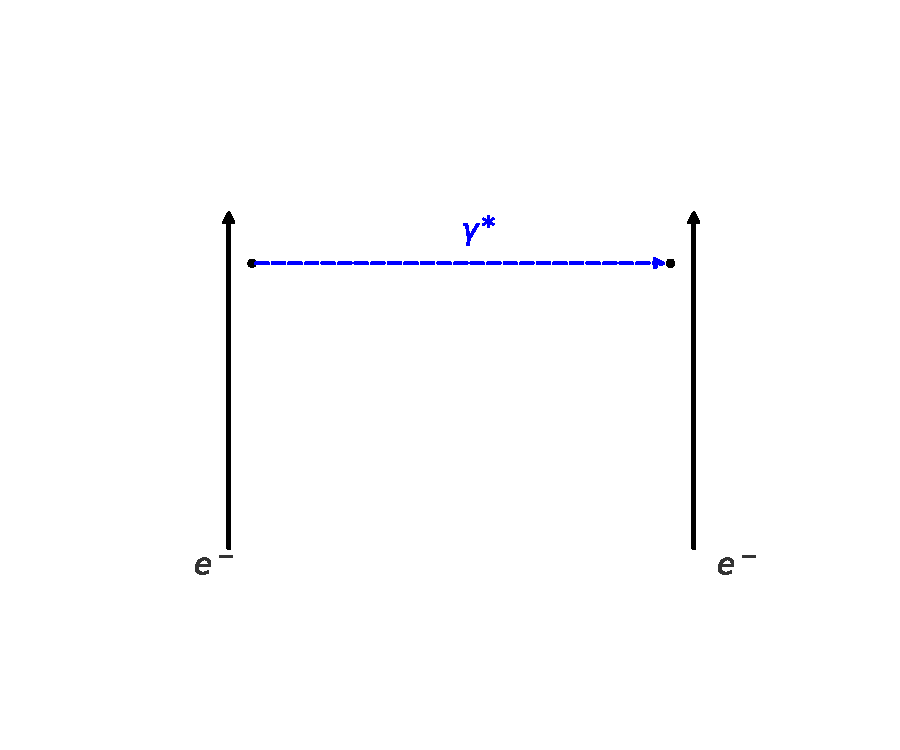
\includegraphics[width=0.4\textwidth]{bilder/moeller-diagramm.pdf}
	\end{center}
	\caption{Das virtuelle Photon ist hier die innere Linie des Feynman-Diagramms. Es vermittelt Impuls – obwohl es niemals real existiert.}
\end{figure}

\subsubsection*{Was zeigt dieses Diagramm?}\index{Feynman-Diagramme!Deutung}\index{Innere Linien (Diagramme)}\index{Vertex}\index{Impulsübertragung}\index{Energieübertragung}
\phantomsection
Das Feynman-Diagramm stellt eine typische \textbf{Møller-Streuung} dar – die elastische Streuung zweier Elektronen durch den Austausch eines virtuellen Photons. Die Zeitachse verläuft dabei von unten nach oben.\index{Zeitachse (Diagramm)}

\begin{itemize}
	\item \textbf{Zwei Elektronen} kommen von unten ins Bild (linke und rechte Seite). Sie bewegen sich aufeinander zu und treten in Wechselwirkung.\index{Elektron}
	
	\item Das \textbf{virtuelle Photon} (gekennzeichnet durch die gestrichelte blaue Linie und das Symbol $\gamma^*$) wird zwischen den Elektronen ausgetauscht.\index{Photon!virtuell $\gamma^*$} Es ist \emph{nicht real}, sondern ein Zwischenzustand der quantenfeldtheoretischen Rechnung.\index{Zwischenzustand}
	
	\item Das Photon überträgt Impuls und Energie – dadurch ändern die Elektronen ihre Bewegungsrichtung und verlassen das Wechselwirkungsgebiet gestreut nach oben.\index{Streuwinkel}
	
	\item Die beiden \textbf{Vertices} (Verbindungspunkte) zeigen, wo die Wechselwirkung lokalisiert ist. Dort findet mathematisch der Impulsübertrag statt.\index{Vertex}
\end{itemize}

\begin{tcolorbox}[didaktikbox, title=Was zeigt das Feynman-Diagramm wirklich?]
	\label{box:Was zeigt das Feynman-Diagramm wirklich}
	Das gezeigte Diagramm der Møller-Streuung zeigt nicht, wie ein reales Photon zwischen Elektronen fliegt. Vielmehr beschreibt es einen quantenmechanischen Übergangszustand:
	
	Ein \textbf{virtuelles Photon} vermittelt die Wechselwirkung – mathematisch im Rahmen der Störungsrechnung. Dieses Photon erfüllt nicht die klassische Beziehung $E = pc$, es existiert nur als \emph{off-shell}-Zwischenzustand und überträgt Impuls.
	
	Reale Effekte wie Streuwinkel und Energieverteilung lassen sich daraus berechnen – ohne dass je ein Photon detektiert wird.
\end{tcolorbox}
\index{Störungsrechnung}\index{Off-shell}\index{Energieverteilung}

\subsubsection*{Keine direkte Beobachtbarkeit – aber messbare Wirkung}\index{Wirkungsquerschnitt}\index{Messgrößen}
\phantomsection
Virtuelle Photonen sind nicht detektierbar. Dennoch beeinflussen sie messbare Größen: Wirkungsquerschnitte, Streuwinkel und Energieverteilungen lassen sich mit hoher Genauigkeit durch die zugrunde liegende Austauschart beschreiben.

\subsubsection*{Abgrenzung zur realen Photonenerzeugung}\index{Compton-Effekt}\index{Photonenprozesse}\index{Austauschdiagramme}\index{Reale Photonen}
\phantomsection
Ein wichtiger Unterschied: Beim \emph{Compton-Effekt} wird ein \textbf{reales} Photon gestreut – mit Nachweis im Detektor. Beim \textbf{virtuellen Austausch} hingegen ist kein Photon als reales Teilchen beteiligt. Das ist der fundamentale Unterschied zwischen \textbf{Austauschdiagrammen} und \textbf{Photonenprozessen}.

\vspace{1em}

% Didaktikbox: Kein klassisches Kraftfeld
\begin{tcolorbox}[didaktikbox, title=Keine „unsichtbare Kraft“ mehr nötig]
	\label{box:unsichtbare Kraft}
	In der Quantenfeldtheorie braucht man kein klassisches Kraftfeld mehr, das zwischen zwei Ladungen wirkt. Stattdessen entstehen Wechselwirkungen durch den Austausch von virtuellen Teilchen – hier: virtuellen Photonen.
	
	Das klassische Bild der Fernwirkung wird so durch ein lokales, quantisiertes Austauschprinzip ersetzt.
\end{tcolorbox}
\index{Fernwirkung}\index{Lokalität}\index{Austauschprinzip}

\subsubsection{Feynman-Diagramme als visuelle Rechenhilfe}\index{Feynman-Diagramme!Rechenhilfe}\index{Wahrscheinlichkeitsamplitude}\index{Störungsrechnung}

Die sogenannten \textbf{Feynman-Diagramme} sind ein zentrales Werkzeug der Quantenfeldtheorie – insbesondere in der Quantenelektrodynamik (QED).\index{Quantenfeldtheorie}\index{QED} Sie dienen als \emph{grafische Notation} für mathematische Terme in der Störungsrechnung und helfen dabei, komplexe Prozesse anschaulich zu strukturieren.

Ein Diagramm stellt keinen realen „Ablauf in Raum und Zeit“ dar, sondern kodiert eine Wahrscheinlichkeitsamplitude. Dennoch lassen sich daraus physikalisch messbare Größen wie Streuwinkel, Wirkungsquerschnitte oder Lebensdauern berechnen.\index{Lebensdauer}

\subsubsection*{Elemente eines Feynman-Diagramms}\index{Fermionlinien}\index{Photonenlinien}\index{Vertices}\index{Zeitachse (Diagramm)}
\phantomsection
\begin{itemize}
	\item \textbf{Fermionlinien:} durchgezogene Linien mit Pfeil – z.\,B. Elektronen oder Positronen
	\item \textbf{Photonenlinien:} wellige oder gestrichelte Linien – je nach Konvention
	\item \textbf{Vertices:} Punkte, an denen Teilchen „wechselwirken“, also Impuls übertragen wird
	\item \textbf{Zeitachse:} meist von unten nach oben oder von links nach rechts
\end{itemize}
\begin{figure}[H]
	\begin{center}
		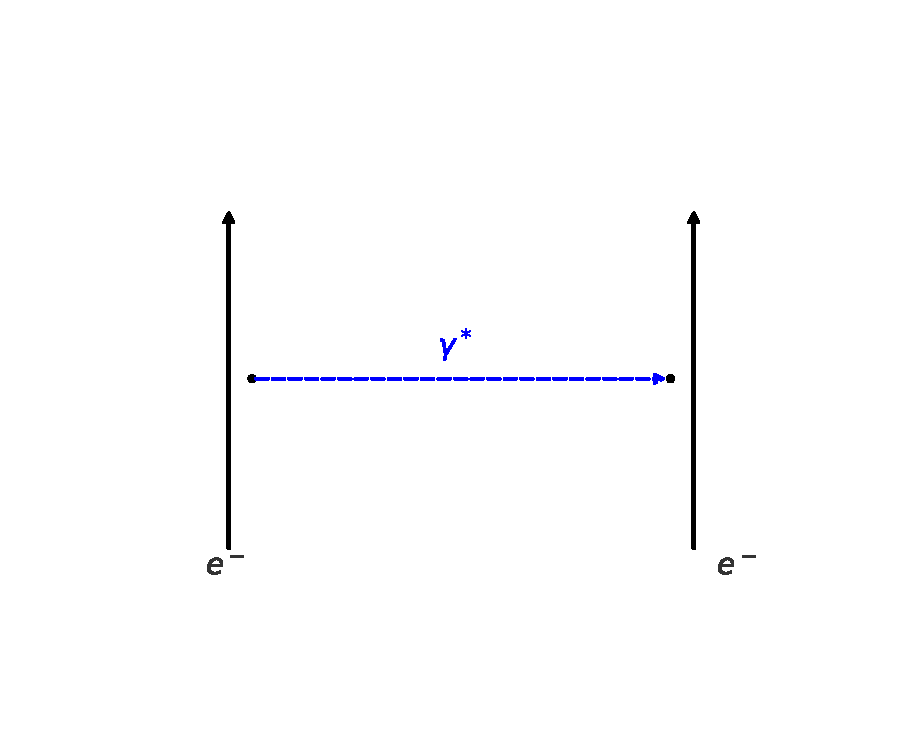
\includegraphics[width=0.45\textwidth]{bilder/feynman-einphoton.pdf}
	\end{center}
	\caption{Feynman-Diagramm}
\end{figure}

\vspace{0.5em}
\begin{tcolorbox}[physikbox, title=Was ein Feynman-Diagramm wirklich zeigt]
	\label{box:Was ein Feynman-Diagramm}
	Ein Feynman-Diagramm ist kein klassischer Bewegungsfilm, sondern eine symbolische Darstellung eines mathematischen Integrals über alle möglichen Pfade eines Prozesses. Es kodiert die Struktur der Wahrscheinlichkeitsamplitude, nicht die exakte Bahn einzelner Teilchen.
\end{tcolorbox}
\index{Pfadintegral}

\subsubsection*{Beispiel: Ein-Photon-Austausch}\index{Ein-Photon-Austausch}\index{Elektron-Elektron-Streuung}\index{Impulsübertrag}
\phantomsection
Beim elastischen Elektron-Elektron-Stoß besteht das zugehörige Feyn\-man-Diagramm aus zwei einlaufenden und zwei auslaufenden Elektronenlinien sowie einer virtuellen Photonenlinie dazwischen. Dieses Diagramm steht symbolisch für eine Formel, die über alle möglichen Impulsüberträge und Zeitpunkte summiert – es ersetzt nicht die Realität, sondern bildet sie probabilistisch ab.\index{Probabilistische Beschreibung}

\subsubsection*{Mehr als nur Bilder – Diagrammregeln}
\phantomsection
\index{Feynman-Regeln}\index{Propagator}\index{Kopplungskonstante}\index{Ladung!elektrische}\index{Amplitude!Streuamplitude}
Jedes Feynman-Diagramm entspricht einem mathematischen Ausdruck. Die sogenannte \emph{Feynman-Regel} weist z.\,B. jeder Linie einen Bruchterm (Propagator), jedem Vertex eine Kopplungskonstante (z.\,B. $e$), und dem Gesamtdiagramm ein Integral über Impulse zu. Die Summe aller möglichen Diagramme bis zu einem bestimmten Ordnungsniveau ergibt die physikalisch messbare Größe.\index{Impulsraum-Integral}\index{Ordnung (Störungstheorie)}

\vspace{1em}
\begin{tcolorbox}[didaktikbox, title=Diagramm ist nicht gleich Realität]
	\label{boxx:Diagramm ist nicht gleich realität}
	Ein häufiges Missverständnis ist, dass ein Feynman-Diagramm einen realen Ablauf zeigt – etwa wie ein Photon „fliegt“. Tatsächlich beschreibt es eine \emph{Überlagerung aller möglichen Zwischenzustände}, zusammengefasst in einer quantenmechanischen Amplitude. Es ist also ein Werkzeug des Rechnens, kein Film des Geschehens.
\end{tcolorbox}
\index{Überlagerung}\index{Zwischenzustand}

\subsubsection{Beispielhafte Diagramme}\index{Prozesse!QED}\index{Virtuelle Photonen!vs.\ reale Photonen}\index{Reale Photonen}
\phantomsection

Um die Rolle virtueller Photonen im Vergleich zu realen Photonen besser zu verstehen, lohnt sich ein Blick auf typische Prozesse in der Quantenelektrodynamik. Feynman-Diagramme zeigen dabei deutlich, ob ein Photon real (detektierbar) oder nur virtuell (vermittelt Wechselwirkung) ist.

\subsubsection*{1. Virtueller Austausch: Møller-Streuung (Elastischer $e^-e^-$-Stoß)}\index{Møller-Streuung}\index{Streuung!elastisch}\index{Virtuelle Photonen!Austausch}
\phantomsection
In diesem Prozess stoßen zwei Elektronen über den Austausch eines virtuellen Photons elastisch aneinander. Das Photon ist nicht real – es vermittelt lediglich Impuls.\index{Impulsübertragung}
\begin{figure}[H]
	\begin{center}
		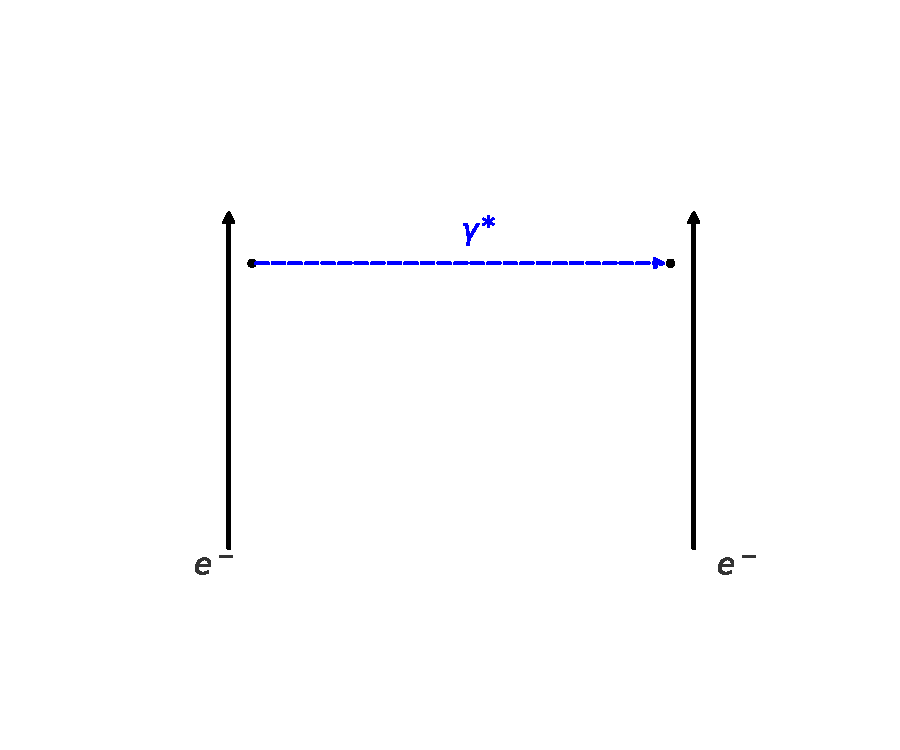
\includegraphics[width=0.42\textwidth]{bilder/moeller-diagramm.pdf}
	\end{center}
	\caption{Virtuelles Photon}
\end{figure}


\begin{tcolorbox}[physikbox, title=Virtuelles Photon]
	\label{box:virtuelles Photon}
	Das ausgetauschte Photon ist virtuell – es existiert nicht als reales Teilchen. Es überträgt Impuls und Energie, erfüllt aber nicht $E = pc$.
\end{tcolorbox}
\index{Photon!virtuell}\index{Energieübertragung}
\subsubsection*{2. Reales Photon: Compton-Streuung}\index{Compton-Effekt}\index{Reale Photonen}\index{Feynman-Diagramme!Compton-Streuung}\index{On-shell}\index{Elektronen-Propagator}\index{Vertex}
\phantomsection
Beim Compton-Effekt wird ein reales Photon an einem Elektron gestreut. Sowohl Ein- als auch Aus-Photon sind reale, detektierbare Teilchen.\index{Detektion} Das Feynman-Diagramm zeigt zwei Vertices mit einem internen Elektronen-Propagator.\index{Propagator!Elektron}\index{Vertices}

\begin{figure}[H]
	\begin{center}
		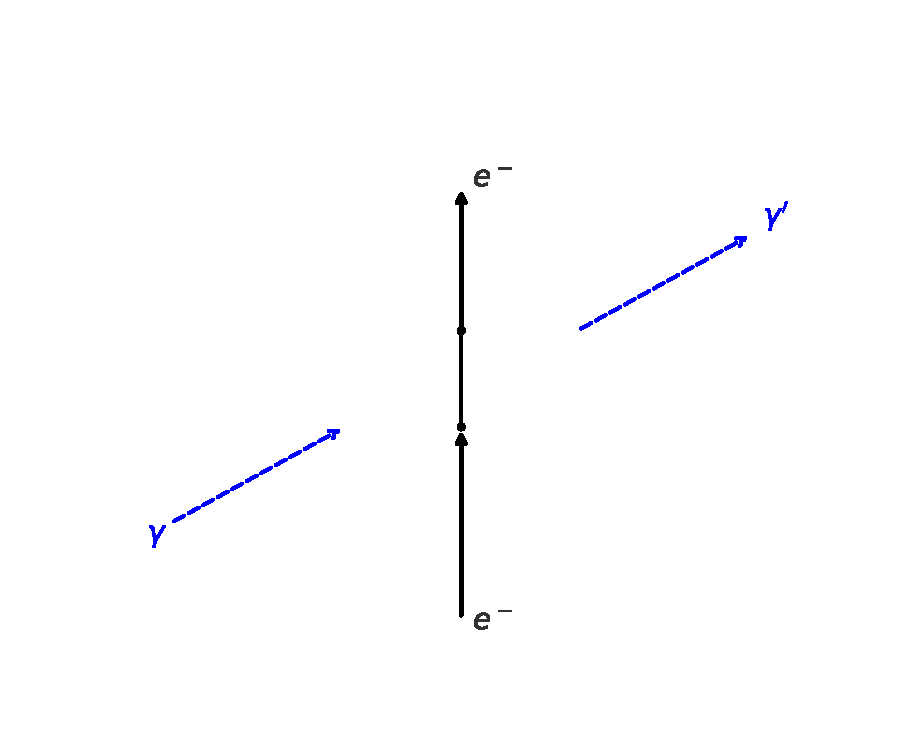
\includegraphics[width=0.5\textwidth]{bilder/compton-diagramm.pdf}
	\end{center}
	\caption{Reales Photon}
\end{figure}

\begin{tcolorbox}[physikbox, title=Reale Photonen]
	\label{box:Reale Photonen}
	In der Compton-Streuung treten Photonen als reale Teilchen auf. Sie sind messbar und erfüllen die on-shell-Bedingung $E = pc$.
\end{tcolorbox}
\index{Photon!real}\index{On-shell-Bedingung}

\subsubsection*{3. Schleifendiagramme: Selbstwechselwirkung und g-Faktor}\index{Schleifendiagramme}\index{Selbstenergie}\index{Vertexkorrektur}\index{g-Faktor!Anomalie}
\phantomsection
In höheren Ordnungen der Störungsrechnung tauchen geschlossene Schleifen in Feynman-Diagrammen auf – etwa bei der Selbstwechselwirkung eines Elektrons mit sich selbst über ein virtuelles Photon.\index{Virtuelle Photonen} Solche Diagramme erklären u.\,a. die Anomalie des $g$-Faktors.\index{Anomalie!$g$-Faktor}
\begin{figure}[H]
	\begin{center}
		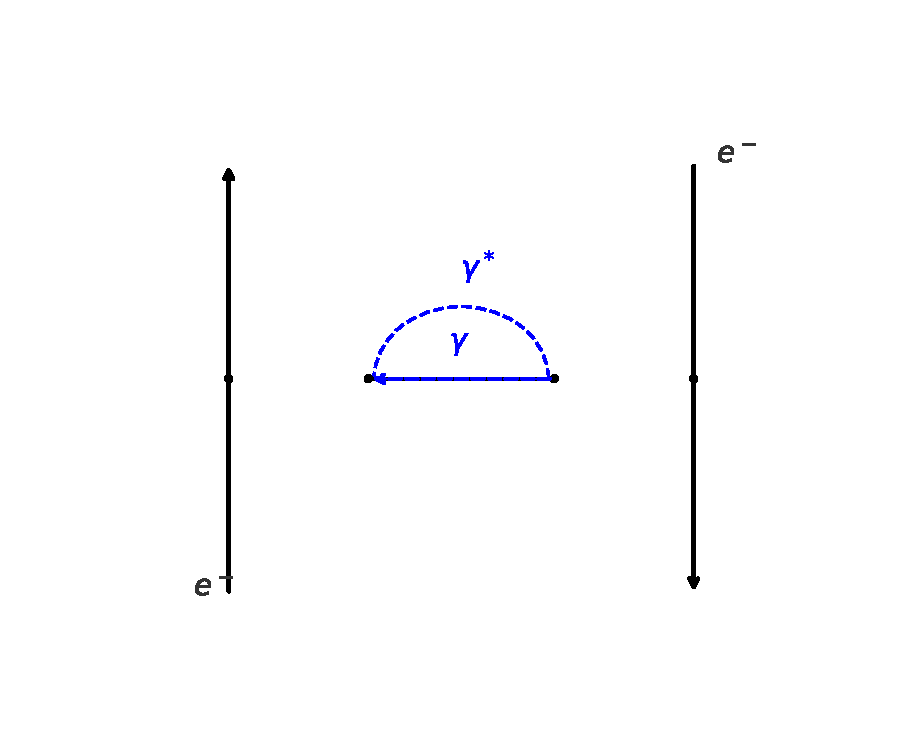
\includegraphics[width=0.4\textwidth]{bilder/vertex-korrektur.pdf}
	\end{center}
	\caption{Schleifendiagramm}
\end{figure}

\begin{tcolorbox}[hinweisbox, title=Schleifendiagramme und Präzisionseffekte]
	\label{box:Schleifendiagramme}
	Schleifen mit virtuellen Photonen liefern Korrekturen zu einfachen Prozessen – etwa für den exakten Wert des Elektron-$g$-Faktors oder den Lamb-Shift. Diese Effekte wurden experimentell mit hoher Präzision bestätigt.
\end{tcolorbox}
\index{Lamb-Shift}\index{Präzisionsexperimente}

\subsubsection*{Didaktischer Vergleich}\index{Didaktischer Vergleich}\index{Photonen!real vs.\ virtuell}
\phantomsection
\begin{itemize}
	\item \textbf{Virtuelle Photonen} treten als innere Linien in Diagrammen auf. Sie sind nicht direkt nachweisbar, aber physikalisch wirksam.\index{Innere Linien}\index{Nachweis!indirekt}
	\item \textbf{Reale Photonen} sind äußere Linien. Sie können gemessen werden und sind on-shell.\index{Äußere Linien}
\end{itemize}

\begin{tcolorbox}[didaktikbox, title=Reale oder virtuelle Photonen im Diagramm]
	\label{box:Reale oder virtuelle Photonen}
	Ob ein Photon real oder virtuell ist, erkennt man daran, ob es als ein- oder auslaufendes Teilchen dargestellt wird. Nur reale Photonen sind beobachtbar. Virtuelle Photonen sind innere Linien – sie „existieren“ nur innerhalb des Rechenwegs.
\end{tcolorbox}
\index{Beobachtbarkeit}\index{Einlaufende Teilchen}\index{Auslaufende Teilchen}

\subsubsection{Bedeutung für die QED}\index{QED!Bedeutung}\index{Elektromagnetische Wechselwirkung}

Die Quantenelektrodynamik (QED) ist die am genauesten bestätigte Theorie der Physik. Ihre enorme Präzision wäre ohne das Konzept der virtuellen Photonen und die Feynman-Diagramme nicht denkbar.\index{Feynman-Diagramme}\index{Virtuelle Photonen}

\subsubsection*{Zentrale Rolle der virtuellen Photonen}\index{Virtuelle Photonen!zentrale Rolle}\index{Störungsrechnung}
\phantomsection
Virtuelle Photonen ermöglichen die Berechnung der elektromagnetischen Wechselwirkung zwischen geladenen Teilchen auf quantenmechanischer Ebene. Sie treten in allen Ordnungen der Störungsrechnung auf – vom einfachen Austausch bis zu komplexen Schleifenprozessen.\index{Austauschprozesse}\index{Loop-Korrekturen}

\vspace{1em}
\begin{tcolorbox}[physikbox, title=Ohne virtuelle Photonen keine QED]
	\label{box:Ohne virtuelle Photonen keine}
	Virtuelle Photonen sind das Fundament der quantenfeldtheoretischen Beschreibung elektromagnetischer Prozesse. Ohne sie könnte die QED keine Kräfte vermitteln und keine quantitativen Vorhersagen machen.
\end{tcolorbox}

\subsubsection*{Feynman-Diagramme als methodisches Rückgrat}\index{Feynman-Diagramme!Methode}\index{Amplituden!Wahrscheinlichkeits-}
\phantomsection
Feynman-Diagramme liefern nicht nur eine anschauliche Darstellung, sondern auch eine präzise Rechenvorschrift. Für jede mögliche Wechselwirkung können alle erlaubten Diagramme gezeichnet und in einen mathematischen Ausdruck übersetzt werden. Die Summe aller Diagramme liefert die beobachtbare Amplitude.\index{Summe über Diagramme}

\subsubsection*{Beispiel: Berechnung des $g$-Faktors}\index{g-Faktor!Elektron}\index{Anomalous magnetic moment}
\phantomsection
Die Abweichung des gyromagnetischen Faktors des Elektrons vom klassischen Wert $g = 2$ ist eines der genauesten Experimente der modernen Physik. Die Korrektur ergibt sich aus einem Schleifenprozess mit einem virtuellen Photon – also aus einem Feynman-Diagramm zweiter Ordnung.\index{Zweite Ordnung}

\subsubsection*{Exaktheit der Theorie}\index{QED!Exaktheit}\index{Vergleich Theorie–Experiment}
\phantomsection
Die theoretisch berechneten Werte für Größen wie den Lamb-Shift, den Elektron-$g$-Faktor oder Streuwinkel in Elektron-Stößen stimmen mit den Messergebnissen auf viele Dezimalstellen überein.\index{Streuwinkel}\index{Elektron-Streuung}
\vspace{1em}
\begin{tcolorbox}[didaktikbox, title=Die Quantenelektrodynamik als Erfolgsmodell]
	\label{box:Die Quantenelekrodynamik}
	Die QED ist nicht nur eine elegante Theorie – sie liefert mit Hilfe virtueller Teilchen und Feynman-Diagrammen quantitative Vorhersagen mit einer Genauigkeit von bis zu 12 Dezimalstellen. Die Rolle des Photons – auch als virtuelles Teilchen – steht dabei im Zentrum.
\end{tcolorbox}
\index{Erfolgsmodell}\index{Genauigkeit!12 Dezimalstellen}

\subsubsection{Grenzen und Missverständnisse}\index{Grenzen der QED}\index{Missverständnisse!Feynman-Diagramme}

Trotz ihrer anschaulichen Darstellung dürfen Feynman-Diagramme nicht als bildliche Beschreibung realer Abläufe missverstanden werden. Virtuelle Photonen existieren nicht im klassischen Sinn – sie sind mathematische Objekte in einer Näherungsrechnung.\index{Näherungsrechnung}

\subsubsection*{Virtuelle Photonen fliegen nicht}\index{Virtuelle Photonen!kein Flug}\index{Teilchenbahn!nicht klassisch}
\phantomsection
Es ist irreführend zu sagen, dass ein virtuelles Photon „zwischen zwei Elektronen hin- und herfliegt“. Virtuelle Teilchen sind nicht messbar, nicht lokalisiert und erfüllen keine klassische Bewegungsgleichung. Ihre Rolle besteht ausschließlich in der Vermittlung von Wechselwirkung innerhalb eines quantenmechanischen Rechenmodells.\index{Lokalisation}\index{Bewegungsgleichung!klassisch}

\vspace{0.5em}
\begin{tcolorbox}[didaktikbox, title=Keine Teilchenbahn im Diagramm]
	\label{box: Keine Teilchenbahn im Diagramm}
	Ein Feynman-Diagramm beschreibt keine Bewegung im Raum und keine klassische Flugbahn. Es stellt eine symbolische Struktur für die Berechnung einer Amplitude dar. Die „Linien“ im Diagramm sind keine Bahnen, sondern Terme in einer Formel.
\end{tcolorbox}
\index{Linien!keine Bahnen}

\subsubsection*{Off-shell heißt: keine Energie-Impuls-Beziehung}\index{Off-shell}\index{Energie-Impuls-Beziehung}
\phantomsection
Virtuelle Photonen erfüllen nicht die bekannte Beziehung $E = pc$. Sie sind \emph{off-shell}, d.\,h. sie verletzen kurzfristig die Energie-Impuls-Bilanz – im Rahmen der Heisenbergschen Unschärferelation.\index{Unschärferelation!Zeit–Energie} Dies ist keine Schwäche der Theorie, sondern eine ihrer zentralen Eigenschaften.

\subsubsection*{Die Diagramme sind keine exakten Abbilder}\index{Feynman-Diagramme!keine Abbilder}\index{Realität!vs.\ Modell}
\phantomsection
Ein weiteres Missverständnis ist die Annahme, Feynman-Diagramme zeigten, „was wirklich passiert“. Tatsächlich enthalten sie keine Aussage über die Reihenfolge von Ereignissen, reale Orte, oder klassische Zeiten. Die Diagramme stehen für Wahrscheinlichkeitsamplituden – nicht für Beobachtungen.\index{Beobachtungen}

\vspace{0.5em}
\begin{tcolorbox}[warnbox, title=Warnung: Feynman-Diagramme nicht wörtlich nehmen!]
	\label{box:Warnung}
	Feynman-Diagramme sind ein mächtiges Rechenwerkzeug – aber keine Realitätsskizzen. Wer sie als „Ablauf von Teilchenflügen“ versteht, verfehlt den Kern der Quantenfeldtheorie.
\end{tcolorbox}
\index{Warnung}

\subsubsection*{Grenzen der Gültigkeit}\index{Gültigkeitsbereich}\index{Starke Wechselwirkung!Grenzen der Störungstheorie}\index{Gittereichtheorie}
\phantomsection
Die QED – und mit ihr das Konzept virtueller Photonen – ist eine Störungstheorie. Sie funktioniert hervorragend bei kleinen Kopplungskonstanten (z.\,B. in der Elektrodynamik), versagt aber bei starker Wechselwirkung. Dort sind andere Methoden (z.\,B. Gittertheorie) notwendig.

\subsubsection*{Fazit dieses Abschnitts}\index{Fazit!virtuelle Photonen und Diagramme}
\phantomsection
Virtuelle Photonen und Feynman-Diagramme sind zentrale Begriffe in der QED – aber sie müssen korrekt interpretiert werden: nicht als „fliegende Teilchen“, sondern als Bausteine einer mathematischen Theorie mit enormer Vorhersagekraft.

\subsubsection{Zusammenfassung}\index{Zusammenfassung!QED-Interpretation}

Virtuelle Photonen erscheinen nicht in Detektoren – aber sie bestimmen, was dort gemessen wird. Sie sind die unsichtbaren Träger der elektromagnetischen Wechselwirkung in der Quantenwelt. Feynman-Diagramme helfen dabei, ihre Wirkung mathematisch zu erfassen, ohne ihnen eine klassische Realität zu unterstellen.

Die QED wäre ohne diese Konzepte nicht möglich – und gerade ihre scheinbar abstrakten Bausteine machen sie zur präzisesten Theorie der Physik.\index{Präziseste Theorie}

\subsection{Der QED-Formalismus}\index{QED!Formalismus}\index{Lagrangedichte!QED}\index{Eichinvarianz}\index{Renormierung@Renormierung (allg.)}
% Kopplungskonstante, Eichinvarianz, Renormierung, Propagatoren

Die Quantenelektrodynamik – kurz QED – ist die Feldtheorie der elektromagnetischen Wechselwirkung.\index{Feldtheorie} Sie beschreibt, wie sich Elektronen, Positronen und Photonen quantenmechanisch verhalten und miteinander wechselwirken.\index{Elektron}\index{Positron}\index{Photon}

Im vorangegangenen Kapitel haben wir gesehen, wie Feynman-Dia\-gramme verwendet werden, um Prozesse wie Elektron-Streuung, Compton-Effekt oder Selbstwechselwirkungen darzustellen.\index{Elektron-Streuung}\index{Compton-Effekt}\index{Selbstwechselwirkung} Doch diese Diagramme sind kein Ersatz für die zugrunde liegende Theorie – sie sind \emph{abgeleitete Werkzeuge}.\index{Werkzeuge!abgeleitete}

In diesem Kapitel gehen wir einen Schritt tiefer: Wir betrachten den \textbf{mathematischen Aufbau} der QED.\index{Mathematischer Aufbau} Im Zentrum steht die sogenannte \textbf{Lagrangedichte}, aus der sich alle Vorhersagen der Theorie ableiten lassen – von der Struktur der Wechselwirkung bis hin zu den Feynman-Regeln.\index{Feynman-Regeln}

Dabei zeigt sich: Die gesamte Quantenelektrodynamik lässt sich aus wenigen Prinzipien aufbauen – insbesondere aus der Forderung nach \textbf{Eichinvarianz} und der \textbf{Relativitätstheorie}.\index{Relativitätstheorie} Diese Prinzipien bestimmen nicht nur die Form der Gleichungen, sondern auch, wie sich das Photon in dieser Theorie als masseloses Wechselwirkungsteilchen einfügt.\index{Photon!masselos}\index{Wechselwirkungsteilchen}

Ziel dieses Kapitels ist es daher, die QED aus ihrem Fundament zu verstehen – nicht als Sammlung von Rechenregeln, sondern als elegant strukturierte Theorie mit enormer Vorhersagekraft.\index{Vorhersagekraft}
\vspace{1em}
\begin{tcolorbox}[hinweisbox, title=Hinweis für Leser:innen]
	\label{box:Hinweis füe Leser}
	Dieses Kapitel führt in die mathematische Struktur der Quantenelektrodynamik (QED) ein. Es richtet sich an Leser:innen mit Interesse an der theoretischen Herleitung der Photonen-Wechselwirkung. 
	
	Wer sich primär für die experimentelle Bestätigung und Anwendungen interessiert, kann direkt mit Kapitel~5.5 fortfahren – ohne den roten Faden des Buches zu verlieren.
\end{tcolorbox}
\newpage
\noindent
\subsubsection{Grundidee der QED als Feldtheorie}\index{Grundidee!QED}\index{Feldtheorie!Grundlagen}

Die Quantenelektrodynamik ist eine \textbf{Feldtheorie}.\index{Feldtheorie} Das bedeutet: Sie beschreibt nicht einzelne Teilchen, sondern Felder, die sich im Raum ausbreiten und miteinander wechselwirken.

Ein Elektron wird nicht als Punktteilchen behandelt, sondern als Anregung eines \emph{Dirac-Feldes}.\index{Dirac-Feld} Auch das Licht – genauer: das Photon – ist in dieser Sichtweise keine Welle und kein klassisches Teilchen, sondern die Anregung eines \emph{elektromagnetischen Feldes}, das selbst quantisiert ist.\index{Elektromagnetisches Feld!quantisiert}

\subsubsection*{Teilchen als Felder}\index{Teilchen als Felder}\index{Fock-Raum}\index{Anregungen}
\phantomsection
Statt den Wechsel von Teilchen zu beschreiben, arbeitet die QED mit Feldern wie:
\begin{itemize}
	\item \textbf{Elektronenfeld} $\psi(x)$ (Dirac-Feld)\index{Elektronenfeld $\psi$}
	\item \textbf{Photonenfeld} $A^\mu(x)$ (Viererpotential)\index{Photonenfeld $A^\mu$}\index{Viererpotential}
\end{itemize}

Der Zustand eines Elektrons (z.\,B. Ort, Impuls, Spin) wird durch eine Wellenfunktion im Dirac-Feld beschrieben.\index{Wellenfunktion}\index{Spin} Ein Photon hingegen ist eine Anregung des quantisierten Feldes $A^\mu$ – genauer: ein \textbf{Fock-Zustand} mit einem Photon.\index{Fock-Zustand}

\subsubsection*{Wechselwirkung über Kopplung der Felder}\index{Wechselwirkung!Kopplung der Felder}
\phantomsection
Die zentrale Idee der QED ist, dass diese beiden Felder \emph{miteinander gekoppelt} werden. Die Wechselwirkung erfolgt nicht direkt zwischen Teilchen, sondern über Terme in der sogenannten \textbf{Lagrangedichte}:\index{Lagrangedichte}
\[
\mathcal{L}_{\text{int}} = -e \, \bar{\psi} \gamma^\mu \psi \, A_\mu
\]
\index{Kopplungsterm $-e\bar\psi\gamma^\mu\psi A_\mu$}

Dieser Ausdruck beschreibt, dass das Elektronenfeld $\psi$ mit dem elektromagnetischen Feld $A_\mu$ koppelt – also „fühlt“, ob ein Photon da ist.\index{Kopplung!Elektron–Photon} Der Kopplungsterm enthält genau die Struktur, die später in den Feynman-Diagrammen als Vertex auftaucht.\index{Vertex}

\vspace{0.5em}
\begin{tcolorbox}[physikbox, title=Feldtheorie statt Teilchenmechanik]
	\label{box:Feldtheorie statt Teilchenmechanik}
	In der QED werden Elektronen und Photonen nicht als klassische Teilchen behandelt, sondern als quantisierte Felder. Ihre Wechselwirkung entsteht durch einen Kopplungsterm in der Lagrangedichte – nicht durch eine klassische Kraft.
\end{tcolorbox}
\index{Teilchenmechanik!vs.\ Feldtheorie}

\subsubsection*{Warum dieser Ansatz notwendig ist}\index{Motivation!QED}\index{Grenzen!klassische Elektrodynamik}
\phantomsection
Die klassische Elektrodynamik (Maxwell-Gleichungen) kann viele Phänomene nicht erklären:\index{Maxwellsche Gleichungen}
\begin{itemize}
	\item Keine quantisierte Energieübertragung\index{Energieübertragung!quantisiert}
	\item Kein Photon-Begriff\index{Photon!Begriff}
	\item Keine Möglichkeit zur Beschreibung von Streuung auf Quantenebene\index{Streuung!Quantenebene}
\end{itemize}

Nur eine quantisierte Feldtheorie erlaubt es, Prozesse wie den Photoeffekt, Compton-Streuung oder die Annihilation von Elektron und Positron korrekt zu beschreiben.\index{Photoeffekt}\index{Compton-Effekt}\index{Annihilation!Elektron–Positron}

\vspace{0.5em}
\begin{tcolorbox}[didaktikbox, title=Warum nicht einfach klassisch?]
	\label{box:Warum nicht einfach klassisch?}
	Die Quantenfeldtheorie erweitert die Quantenmechanik auf Systeme mit variabler Teilchenzahl. Nur so lassen sich Erzeugung und Vernichtung von Photonen oder Elektronen mathematisch sauber beschreiben. Ohne diesen Zugang könnte man keine Feynman-Diagramme herleiten – und keine Präzisionsergebnisse der QED erzielen.
\end{tcolorbox}
\index{Quantenfeldtheorie}\index{Quantenmechanik}\index{Erzeugung und Vernichtung}

\subsubsection{Die QED-Lagrangedichte}\index{Lagrangedichte!QED}

Im Zentrum der QED steht die sogenannte \textbf{Lagrangedichte}, aus der sich alle Gleichungen der Theorie ableiten lassen. Sie enthält sowohl die freien Felder (Elektron, Photon) als auch deren Wechselwirkung.

Die vollständige QED-Lagrangedichte lautet:
\[
\mathcal{L}_{\text{QED}} = \bar{\psi}(i \gamma^\mu \partial_\mu - m)\psi - \frac{1}{4}F_{\mu\nu}F^{\mu\nu} - e \bar{\psi} \gamma^\mu \psi A_\mu
\]

\begin{tcolorbox}[mathebox, title=Aufbau der QED-Lagrangedichte]
	\label{box:Sufbau der QED-Langrangedichte}
	\begin{itemize}
		\item $\bar{\psi}(i \gamma^\mu \partial_\mu - m)\psi$: Dirac-Term für das freie Elektronenfeld\index{Dirac-Term}
		\item $-\frac{1}{4}F_{\mu\nu}F^{\mu\nu}$: Kinetischer Term für das Photon (Maxwell-Teil)\index{Maxwell-Term}\index{Kinetischer Term}
		\item $-e \bar{\psi} \gamma^\mu \psi A_\mu$: Kopplung zwischen Elektronenfeld und elektromagnetischem Feld\index{Kopplung!Elektron–Photon}
	\end{itemize}
\end{tcolorbox}

\subsubsection*{Bedeutung der Terme}\index{Termdeutung}\index{Freies Feld}
\phantomsection
Jeder Teil der Lagrangedichte steht für eine Komponente der Theorie:

- Der erste Term beschreibt das \textbf{freie Dirac-Feld} – also ein Elektron oder Positron ohne äußere Einflüsse.\index{Freies Dirac-Feld}
- Der zweite Term ist die \textbf{freie elektromagnetische Feldstärke} – die Quantenversion des Maxwell-Feldes.\index{Freies Photonenfeld}
- Der dritte Term beschreibt die \textbf{Wechselwirkung} zwischen Elektron und Photon – das Herzstück der QED.\index{Wechselwirkung!Elektron–Photon}

\subsubsection*{Feldstärketensor}\index{Feldstärketensor $F_{\mu\nu}$}
\phantomsection
Der Ausdruck $F_{\mu\nu}$ ist der sogenannte \textbf{Feldstärketensor}, definiert als:
\[
F_{\mu\nu} = \partial_\mu A_\nu - \partial_\nu A_\mu
\]
\index{Lorentzinvarianz}

Er enthält sowohl das elektrische als auch das magnetische Feld – verpackt in ein einziges relativistisches Objekt. Der Term $F_{\mu\nu}F^{\mu\nu}$ ist dabei invariant unter Lorentztransformationen.

\vspace{1em}
\begin{tcolorbox}[physikbox, title=Photonenfeld aus der Lagrangedichte]
	\label{box:Photonenfeld aus der Lagrangedichte}
	Die Lichtquanteneigenschaft des Photons ergibt sich in der QED durch die Quantisierung des Feldes $A^\mu$ in der Maxwell-Struktur. Der Feldstärketensor $F_{\mu\nu}$ enthält die Dynamik des Photons als quantisiertes Eichfeld.
\end{tcolorbox}
\index{Eichfeld}

\subsubsection*{Wechselwirkung als Kopplungsterme}\index{Wechselwirkung!Kopplungsterme}\index{QED-Vertex}
\phantomsection
Der Wechselwirkungsterm\\$-e \bar{\psi} \gamma^\mu \psi A_\mu$ beschreibt die Kopplung der Elektronen an das Photon. 
\newpage
\noindent
Aus diesem Term folgt direkt die Struktur des QED-Vertices in Feynman-Diagrammen:
\begin{figure}[H]
	
	\[
	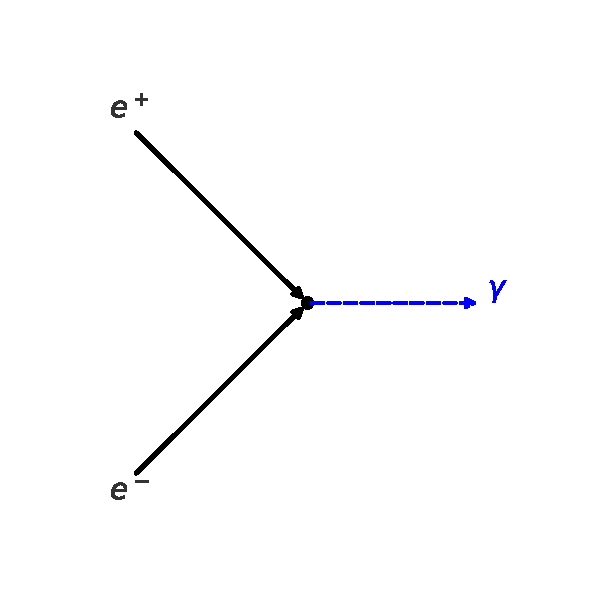
\includegraphics[height=8.5em]{bilder/qed-vertex.pdf} \quad \Rightarrow \quad -ie\gamma^\mu
	\]
	\caption{Wechselwirkungsterm}
\end{figure}
\vspace{0.5em}
\begin{tcolorbox}[didaktikbox, title=Vom Lagrange-Term zum Feynman-Vertex]
	\label{box:Vom Lagrange-Term zum Feynmann-Vertax}
	Die Kopplung in der Lagrangedichte erzeugt das QED-Vertex: ein Elektron, ein Positron, ein Photon treffen an einem Punkt zusammen. Diese Struktur bildet die Grundlage aller Diagramme in der QED.
\end{tcolorbox}
\index{Vertexfaktor $-ie\gamma^\mu$}

\subsubsection*{Eichinvarianz als Prinzip}\index{Eichinvarianz!lokal}\index{Eichtransformation}
\phantomsection
Die Form der QED-Lagrangedichte ist nicht beliebig gewählt. Sie ist das Resultat der Forderung, dass die Theorie \textbf{lokal eichinvariant} ist – also symmetrisch unter Transformationen der Form:
\[
\psi(x) \rightarrow e^{i\alpha(x)} \psi(x), \qquad A_\mu(x) \rightarrow A_\mu(x) - \frac{1}{e} \partial_\mu \alpha(x)
\]

Nur mit dieser Struktur bleibt die Theorie konsistent, relativistisch invariant und quantisierbar.\index{Quantisierbarkeit}

\subsubsection{Kopplung zwischen Elektronen und Photonen}\index{Kopplung!Elektronen–Photonen}\index{Lokale Eichinvarianz}

Die Wechselwirkung zwischen Elektron und Photon ergibt sich in der QED nicht „von außen“, sondern folgt aus einem fundamentalen Prinzip: der \textbf{lokalen Eichinvarianz}. Diese Symmetrie zwingt uns, das Photon als Kopplungspartner des Elektronenfeldes einzuführen.

\subsubsection*{Globale und lokale Phasentransformation}\index{Phasentransformation!global}\index{Phasentransformation!lokal}
\phantomsection
Ein Dirac-Feld $\psi$ ist invariant unter einer \textbf{globalen} Phasentransformation:
\[
\psi(x) \rightarrow e^{i\alpha} \psi(x)
\]
Die Lagrangedichte bleibt dabei unverändert – es handelt sich um eine Symmetrie.

Wenn man aber verlangt, dass $\alpha$ vom Ort abhängt, also
\[
\psi(x) \rightarrow e^{i\alpha(x)} \psi(x)
\]
spricht man von einer \textbf{lokalen Eichtransformation}. Diese zerstört die Invarianz der Lagrangedichte – es sei denn, man führt ein zusätzliches Feld $A_\mu(x)$ ein, das sich mittransformiert:
\[
A_\mu(x) \rightarrow A_\mu(x) - \frac{1}{e} \partial_\mu \alpha(x)
\]

\subsubsection*{Kovarianter Ableiter und minimaler Ersatz}\index{Kovarianter Ableiter}\index{Minimaler Ersatz}
\phantomsection
Damit die Theorie lokal eichinvariant bleibt, ersetzt man in der Dirac-Lagrangedichte die gewöhnliche Ableitung durch den \textbf{kovarianten Ableiter}:
\[
\partial_\mu \rightarrow D_\mu = \partial_\mu + ie A_\mu
\]

Dadurch entsteht automatisch ein Wechselwirkungsterm in der Lagrangedichte:
\[
\mathcal{L}_{\text{int}} = -e \, \bar{\psi} \gamma^\mu \psi A_\mu
\]

\vspace{0.5em}
\begin{tcolorbox}[mathebox, title=Kopplung aus Prinzip]
	\label{box:Kopplung aus Prinzip}
	Die Kopplung zwischen Elektron und Photon ist kein zusätzlicher Term, sondern folgt zwangsläufig aus der Forderung nach lokaler Eichinvarianz. Sie bestimmt die Form der Wechselwirkung eindeutig.
\end{tcolorbox}
\index{Viererstromdichte $\bar\psi\gamma^\mu\psi$}

\subsubsection*{Physikalische Bedeutung}\index{Physikalische Bedeutung!Kopplung}
\phantomsection
Der Ausdruck $\bar{\psi} \gamma^\mu \psi$ ist die \textbf{Viererstromdichte} des Elektronenfeldes. Der Term $A_\mu$ koppelt sich an diesen Strom – genau wie ein klassisches elektromagnetisches Feld an einen elektrischen Strom koppelt. Nur dass hier beide Größen quantisiert sind.\index{Strom!elektrisch}

\subsubsection*{Einfaches Bild: „Feld fühlt Feld“}\index{Anschauliches Bild}\index{Feld koppelt an Feld}
\phantomsection
Man kann sich den Prozess so vorstellen: Das Elektronenfeld „spürt“ das Photonfeld – weil seine Ableitung modifiziert wird. Wo früher nur der Gradient stand, steht nun ein Zusammenhang, der auch das Photon einbezieht.

\vspace{1em}
\begin{tcolorbox}[didaktikbox, title=Die Kraft entsteht aus dem Ableiter]
	\label{box:Die Kraft entsteht aus dem Ableiter}
	Die elektromagnetische Wechselwirkung entsteht in der QED dadurch, dass das Elektronenfeld auf den \emph{kovarianten} Ableiter reagiert. Dieser enthält das Photon – und damit ist die Kopplung erzeugt.
\end{tcolorbox}
\index{Kraft!Ursprung in $D_\mu$}

\subsubsection{Feynman-Regeln aus der Lagrangedichte}\index{Feynman-Regeln}\index{Störungstheorie}

Die Feynman-Diagramme sind keine bloßen Skizzen – sie folgen aus der Struktur der Lagrangedichte. Jeder Term der QED-Lagrangedichte hat eine klare Entsprechung in einem Baustein der Diagramme.

\subsubsection*{Grundprinzip: Störungsentwicklung}\index{Störungsentwicklung}\index{Feinstrukturkonstante $\alpha$}
\phantomsection
Da die Wechselwirkung in der QED schwach ist (die Feinstrukturkonstante $\alpha \approx 1/137$ ist klein), kann man physikalische Größen wie Übergangswahrscheinlichkeiten oder Streuamplituden als \textbf{Reihe in der Kopplungskonstanten} entwickeln. Jedes Glied dieser Reihe entspricht einem Feynman-Diagramm.\index{Übergangswahrscheinlichkeit}\index{Streuamplitude}

\subsubsection*{Elemente und ihre Bedeutung}\index{Propagator}\index{Vertex}\index{Impulsintegral}
\phantomsection
Aus der Lagrangedichte ergeben sich die folgenden Zuordnungen:

\vspace{0.5em}
\begin{tcolorbox}[mathebox, title=Feynman-Regeln der QED (vereinfacht)]
	\label{box:Feynman-Regeln der QED}
	\begin{itemize}
		\item \textbf{Elektronenlinie:} $\displaystyle \frac{i(\slashed{p} + m)}{p^2 - m^2 + i\varepsilon}$ (Dirac-Propagator)\index{Dirac-Propagator}
		\item \textbf{Photonenlinie:} $\displaystyle \frac{-ig^{\mu\nu}}{q^2 + i\varepsilon}$ (Photon-Propagator)\index{Photon-Propagator}
		\item \textbf{Vertex:} $-ie\gamma^\mu$\index{Vertexfaktor $-ie\gamma^\mu$}
		\item \textbf{Jede innere Linie:} Integration über Viererimpuls $d^4p$\index{Viererimpuls!Integration}
		\item \textbf{Gesamtdiagramm:} Produkt aller Faktoren, Integration über Schleifenimpulse\index{Schleifenimpuls}
	\end{itemize}
\end{tcolorbox}

\subsubsection*{Beispiel: Ein-Photon-Austausch}\index{Ein-Photon-Austausch}\index{Møller-Streuung}
\phantomsection
Die einfachste Anwendung ist die Møller-Streuung (Elektron-Elektron-Streuung über ein virtuelles Photon). Aus dem Vertex $-ie\gamma^\mu$ und den Propagatoren ergibt sich die Formel zur Streuamplitude. Die Berechnung folgt direkt aus den Feynman-Regeln – und liefert messbare Größen wie Wirkungsquerschnitte und Streuwinkel.\index{Wirkungsquerschnitt}

\subsubsection*{Ordnung der Diagramme}\index{Ordnung!in $e$}\index{Ordnung!in $\alpha$}\index{Loop-Korrekturen}
\phantomsection
Je mehr Vertices ein Diagramm enthält, desto höher ist seine Ordnung in $e$ bzw. in $\alpha = e^2 / (4\pi\hbar c)$. Niedrigere Ordnungen liefern die Hauptbeiträge, höhere Ordnungen die Korrekturen – etwa in Form von Schleifen (Loop-Korrekturen).

\vspace{1em}
\begin{tcolorbox}[didaktikbox, title=Warum die Regeln funktionieren]
	\label{box:Warum die Regeln funktionieren}
	Die Feynman-Regeln ergeben sich systematisch aus der QED-Lagrangedichte durch Anwendung der Störungstheorie. Sie sind also keine Ansammlung willkürlicher Anweisungen – sondern das direkte Resultat der Struktur der Theorie.
\end{tcolorbox}

\subsubsection*{Zusammenhang zur Messung}\index{Messung!Zusammenhang}\index{Theorie–Experiment}
\phantomsection
Jede beobachtbare Größe – Streuwinkel, Energieverteilung, g-Faktor-Korrektur – lässt sich mit Hilfe der Feynman-Regeln berechnen. Die Übereinstimmung mit dem Experiment macht die QED zur präzisesten Theorie der Physik.\index{Energieverteilung}

\subsubsection{Quantisierung des elektromagnetischen Feldes}\index{Quantisierung!elektromagnetisches Feld}\index{Photon!als Anregung}

In der klassischen Elektrodynamik ist das elektromagnetische Feld durch das Viererpotential $A^\mu(x)$ beschrieben. Doch solange dieses Feld nur klassische Gleichungen erfüllt (z.\,B. die Maxwell-Gleichungen), gibt es keine Photonen. Erst durch \textbf{Quantifizierung} wird aus dem Feld ein Quantensystem – und das Photon tritt als \emph{Anregung} dieses Feldes auf.\index{Maxwellsche Gleichungen}

\subsubsection*{Von der Welle zum Photon}\index{Moden!Quantisierung}\index{Fock-Raum}
\phantomsection
Das elektromagnetische Feld besteht aus unendlich vielen schwingenden Freiheitsgraden – ähnlich wie ein Gitarrensaite mit unendlich vielen möglichen Obertönen. Jeder Modus kann quantisiert werden. Dabei entsteht ein sogenannter \textbf{Fock-Raum}, in dem man Zustände wie
\[
\lvert 0 \rangle, \quad \lvert 1_{\vec{k}} \rangle, \quad \lvert 2_{\vec{k}} \rangle, \quad \dots
\]
beschreibt – also Zustände mit null, einem oder mehreren Photonen einer bestimmten Wellenzahl $\vec{k}$.\index{Vakuumzustand}\index{Photonenzahlzustand}

\subsubsection*{Das Photon als Anregung}\index{Photon!Quantenzustand}\index{Impuls $\hbar\vec{k}$}\index{Energie $\hbar\omega$}
\phantomsection
Ein Photon ist nichts anderes als ein Zustand mit einer einzigen Anregung des quantisierten Feldes $A^\mu(x)$ in einem bestimmten Modus. Diese Sichtweise ist grundlegend anders als die klassische Vorstellung einer Welle oder eines Teilchens.

\vspace{0.5em}
\begin{tcolorbox}[physikbox, title=Was ist ein Photon in der QED?]
	\label{box:Warum ist ein Photon in der QED}
	Ein Photon ist die einfachste Anregung des quantisierten elektromagnetischen Feldes. Es besitzt keine Ruhemasse, aber eine definierte Energie $E = \hbar \omega$ und einen Impuls $\vec{p} = \hbar \vec{k}$.
\end{tcolorbox}

\subsubsection*{Polarisation und Transversalität}\index{Polarisation}\index{Transversalität}\index{Helizität}
\phantomsection
Da das Photon masselos ist, hat es nur zwei physikalisch beobachtbare Polarisationszustände – nicht drei, wie bei einem massiven Spin-1-Teilchen. Das ist eine direkte Konsequenz der Eichinvarianz und der Transversalität der Welle:
\[
\vec{k} \cdot \vec{\epsilon} = 0
\]

Die QED behandelt dies korrekt durch den sogenannten \textbf{Gupta-Bleuler-Formalismus}\index{Gupta-Bleuler-Formalismus} oder über Feynman-Gaugen, bei denen auch unphysikalische Freiheitsgrade zunächst mitgeführt und später herausgerechnet werden.\index{Feynman-Gauß@Feynman-Gauge}

\subsubsection*{Eichsymmetrie und Freiheitsgrade}\index{Eichsymmetrie}\index{Freiheitsgrade}
\phantomsection
Die Eichsymmetrie erlaubt es, bestimmte Komponenten des Feldes $A^\mu$ durch Transformationen zu eliminieren. Physikalisch relevant bleiben nur die transversalen Anteile – und das sind genau die zwei Polarisationsrichtungen des Photons.

\vspace{1em}
\begin{tcolorbox}[didaktikbox, title=Warum hat das Photon keinen Spin-3-Zustand?]
	\label{box:Warum hat das Photon keinen Spin-3-Zustand}
	Ein massives Spin-1-Teilchen hätte drei Polarisationszustände. Aber weil das Photon masselos ist und das elektromagnetische Feld eichinvariant ist, bleiben nur zwei Zustände übrig. Diese entsprechen linearer oder zirkularer Polarisation.
\end{tcolorbox}

\index{Spin!Photon}\index{Zirkulare Polarisation}\index{Lineare Polarisation}

\subsubsection{Zusammenfassung}\index{Zusammenfassung!QED-Formalismus}
\addcontentsline{toc}{subsubsection}{Zusammenfassung}

Die Quantenelektrodynamik (QED) ist die quantisierte Feldtheorie der elektromagnetischen Wechselwirkung. Ihre mathematische Struktur basiert auf folgenden zentralen Elementen:

\begin{itemize}
	\item \textbf{Feldbeschreibung:} Elektronen und Positronen werden durch das Dirac-Feld $\psi(x)$ beschrieben, das Photon durch das Viererpotential $A^\mu(x)$.\index{Dirac-Feld}\index{Viererpotential}
	
	\item \textbf{Lagrangedichte:} Die QED-Lagrangedichte enthält drei Bestandteile:
	\begin{itemize}
		\item den freien Dirac-Term für das Elektronenfeld,\index{Dirac-Term}
		\item den freien Maxwell-Term für das Photonenfeld (Feldstärketensor $F_{\mu\nu}$),\index{Maxwell-Term}\index{Feldstärketensor $F_{\mu\nu}$}
		\item und den Kopplungsterm $-e \bar{\psi} \gamma^\mu \psi A_\mu$.\index{Kopplungsterm $-e\bar\psi\gamma^\mu\psi A_\mu$}
	\end{itemize}
	
	\item \textbf{Kopplung über Eichsymmetrie:} Die Form des Wechselwirkungsterms ergibt sich aus der Forderung lokaler Eichinvarianz. Sie erfordert die Einführung eines kovarianten Ableiters.\index{Kovarianter Ableiter}
	
	\item \textbf{Feynman-Regeln:} Aus der Lagrangedichte lassen sich die Bausteine der Feynman-Diagramme ableiten: Propagatoren, Vertices und Integrationsvorschriften.\index{Propagator}\index{Vertex}\index{Integrationsvorschriften}
	
	\item \textbf{Quantisierung des Photonenfeldes:} Durch Quantisierung des elektromagnetischen Feldes entstehen Photonen als Anregungen – mit zwei physikalischen Polarisationszuständen.\index{Quantisierung!Photonenfeld}\index{Polarisation!Photon}
	
\end{itemize}

Die QED ist in sich konsistent, relativistisch invariant, und stimmt in allen bisher getesteten Bereichen mit der experimentellen Realität überein.\index{Konsistenz}\index{Lorentzinvarianz} Die konkrete Berechnung physikalischer Größen erfolgt über Störungsreihen und Feynman-Diagramme – sie ist Thema des nächsten Kapitels.\index{Störungsreihen}

\subsection{Präzisionsexperimente}\index{Präzisionsexperimente}\index{Tests!QED}

In diesem Abschnitt soll die Rolle des Photons in modernen Hochpräzisionsexperimenten beleuchtet werden.\index{Photon!Rolle in Experimenten} Solche Experimente liefern nicht nur beeindruckende Bestätigungen der Quantenelektrodynamik (QED), sondern auch der speziellen Relativitätstheorie und fundamentaler Symmetrien der Natur.\index{Spezielle Relativitätstheorie}\index{Symmetrien!fundamental} Das Photon ist dabei nicht nur Objekt der Beobachtung, sondern oft auch das zentrale Werkzeug zur Untersuchung feinster physikalischer Effekte.\index{Photon!Messwerkzeug}

\subsubsection{Der anomale magnetische Moment des Elektrons}\index{Magnetisches Moment!anomales}\index{g-Faktor!Elektron}

Eines der am genauesten getesteten Ergebnisse der QED ist das sogenannte \emph{anomalous magnetic moment} des Elektrons, also die kleine Abweichung des $g$-Faktors von exakt 2:
\[
g_e \approx 2{,}00231930436...
\]
Diese Abweichung resultiert aus quantenfeldtheoretischen Korrekturen, insbesondere aus dem Austausch virtueller Photonen:\index{Korrekturen!quantenfeldtheoretisch}\index{Virtuelle Photonen!Schleifen}
\vspace{1em}
\begin{tcolorbox}[physikbox,title=Physikalische Bedeutung]
	\label{box:physikalische Bedeutung}
	Die Differenz von $g_e = 2$ zu dem experimentell gemessenen Wert wird durch Schleifenprozesse in Feynman-Diagrammen erklärt, bei denen virtuelle Photonen zwischen Elektron und sich selbst vermittelt werden. Die Übereinstimmung zwischen Theorie und Experiment ist ein Triumph der QED.
\end{tcolorbox}
\index{Triumph der QED}

\subsubsection{Lamb-Verschiebung}\index{Lamb-Shift}\index{Wasserstoff!Spektrum}

Ein weiteres spektakuläres Beispiel für die experimentelle Bestätigung der QED ist die \emph{Lamb-Verschiebung} der Energieniveaus im Wasserstoffatom. Der klassische Dirac-Formalismus sagt für das 2s- und 2p-Niveau dieselbe Energie voraus. Experimentell wurde jedoch eine winzige Energieverschiebung festgestellt:
\[
\Delta E_\text{Lamb} \approx \SI{1057}{\mega\hertz}
\]
\vspace{0.5em}
\begin{tcolorbox}[didaktikbox,title=Warum ist das wichtig?]
	\label{box:Warum ist wichtig}
	Die Lamb-Verschiebung zeigt, dass der leere Raum – das Quantenvakuum – nicht „leer“ ist. Virtuelle Photonen bewirken Fluktuationen, die die Energieniveaus beeinflussen.
\end{tcolorbox}
\index{Quantenvakuum}\index{Vakuumfluktuationen}
\subsubsection{Spektroskopie und Konstanzmessungen}\index{Spektroskopie}\index{Naturkonstanten!Messungen}\index{Frequenzkamm}\index{Atomuhr}

Photonenbasierte Hochpräzisions-Spektroskopie liefert auch genaueste Messungen fundamentaler Naturkonstanten wie:

\begin{itemize}
	\item der Feinstrukturkonstante $\alpha$\index{Feinstrukturkonstante $\alpha$}
	\item der Planck-Konstante $h$\index{Planck-Konstante $h$}
	\item der Lichtgeschwindigkeit $c$ (heute fest definiert)\index{Lichtgeschwindigkeit $c$}
\end{itemize}

Diese Messungen stützen sich auf Lasertechnologie, Frequenzkämme und Atomuhren – allesamt photonengebundene Techniken.\index{Laser}\index{Photonentechniken}

\subsubsection{Tests fundamentaler Symmetrien}\index{Symmetrien!Tests}\index{CPT-Invarianz}\index{Lorentz-Invarianz}

Experimente mit Photonen tragen dazu bei, fundamentale Symmetrien zu testen:

\begin{itemize}
	\item \textbf{CPT-Invarianz:} Präzisionsmessungen am Antiwasserstoff vergleichen Spektrallinien mit gewöhnlichem Wasserstoff.\index{Antiwasserstoff}
	\item \textbf{Lorentz-Invarianz:} Richtungsabhängigkeiten der Lichtgeschwindigkeit werden mit resonatorgestützten Lasersystemen überprüft.\index{Resonator!optisch}
\end{itemize}
\vspace{0.5em}
\begin{tcolorbox}[hypobox, title={Was wäre, wenn Licht nicht isotrop wäre?}]
	\label{box:was wäre nicht isotop}
	
	Würde man eine Richtungsabhängigkeit der Lichtgeschwindigkeit messen, wäre das ein Hinweis auf eine fundamentale Verletzung der Lorentz-Symmetrie – mit drastischen Folgen für die Relativitätstheorie und unser physikalisches Weltbild.
\end{tcolorbox}
\index{Isotropie des Lichts}\index{Lorentz-Symmetrie!Verletzung}

\subsubsection{Zusammenfassung}\index{Zusammenfassung!Präzisionsexperimente}

Präzisionsexperimente sind eine der stärksten Säulen zur Überprüfung unserer physikalischen Theorien. Sie zeigen, wie weitreichend und verlässlich das Konzept des Photons in der modernen Physik verankert ist. Besonders die Quantenelektrodynamik beweist hier ihre beispiellose Genauigkeit – und mit ihr die zentrale Rolle des Photons als Austauschteilchen und Informationsträger.\index{Informationsträger!Photon}

\subsection{Fazit}
% Zusammenfassung der Rolle des Photons in der QED, Übergang zu Kapitel VI

In Kapitel~V haben wir das Photon als zentrales Vermittlungsteilchen der elektromagnetischen Wechselwirkung im Rahmen der Quantenelektrodynamik (QED) kennengelernt.\index{Vermittlungsteilchen} Beginnend mit dem Übergang vom klassischen Lichtquant zum quantisierten Feld wurde deutlich, wie tief die Struktur der QED mit dem Photon verknüpft ist. 

Wir haben gesehen:
\begin{itemize}
	\item wie sich das Photon mathematisch als Vektorfeld mit Eichfreiheit beschreiben lässt,\index{Vektorfeld!Photon}\index{Eichfreiheit}
	\item wie virtuelle Photonen in Feynman-Diagrammen die Wechselwirkung zwischen geladenen Teilchen vermitteln,\index{Virtuelle Photonen!Vermittlung}
	\item wie der QED-Formalismus über Eichsymmetrie, Lagrangedichte und Störungstheorie aufgebaut ist,\index{QED!Aufbau}\index{Störungstheorie}
	\item und wie Präzisionsexperimente – vom $g$-Faktor bis zur Lamb-Verschiebung – die Theorie mit beispielloser Genauigkeit bestätigen.\index{Bestätigung!experimentell}
\end{itemize}

Die Quantenelektrodynamik zählt zu den erfolgreichsten Theorien der Physik. Sie liefert nicht nur präzise Vorhersagen, sondern auch ein tiefes Verständnis der Rolle des Photons – als masseloses, aber wirkungsmächtiges Quantenobjekt.\index{Quantenobjekt!Photon} 

\vspace{1em}
\begin{tcolorbox}[hinweisbox,title=Ausblick auf Kapitel VI]
	\label{box:Ausblick auf Kapitel 6}
	Im nächsten Kapitel betrachten wir Anwendungen des Photons in Praxis und Forschung – von der Lasertechnologie über Quantensensoren bis zur Rolle in der modernen Kommunikation.
\end{tcolorbox}
\index{Lasertechnologie}\index{Quantensensorik}\index{Quantenkommunikation}

	\chapter{Anwendungen des Photons}

\setcounter{section}{6}
\setcounter{subsection}{0}
\setcounter{subsubsection}{1}
\setcounter{secnumdepth}{3}
% Boxen-Stile definieren
\tcbset{physikbox/.style={colback=blue!5!white, colframe=blue!75!black, fonttitle=\bfseries}}
\tcbset{mathebox/.style={colback=green!5!white, colframe=green!50!black, fonttitle=\bfseries}}
\tcbset{didaktikbox/.style={colback=yellow!5!white, colframe=yellow!50!black, fonttitle=\bfseries}}
\tcbset{hypobox/.style={colback=orange!5!white, colframe=orange!75!black, fonttitle=\bfseries}}
\tcbset{hinweisbox/.style={colback=gray!10!white, colframe=black!40!black, fonttitle=\bfseries}}

\subsection{Einleitung}

Photonen\index{Photon} sind nicht nur fundamentale Träger quantenphysikalischer Eigenschaften\index{Quantenphysikalische Eigenschaft} – sie bilden auch die Grundlage zahlreicher Anwendungen\index{Anwendung} in Technik\index{Technik}, Forschung\index{Forschung} und Alltag. In diesem Kapitel werden ausgewählte Einsatzfelder vorgestellt, in denen die Kontrolle\index{Photonenkontrolle}, Detektion\index{Photonendetektion} und Nutzung\index{Photonennutzung} einzelner Photonen eine zentrale Rolle spielt. Die Spannweite reicht von Lasertechnologie\index{Lasertechnologie} und Quantensensorik\index{Quantensensorik} über medizinische Bildgebung\index{Medizinische Bildgebung} bis hin zur optischen Kommunikation\index{Optische Kommunikation} und astronomischen Beobachtung\index{Astronomische Beobachtung}. Ziel ist es, die physikalischen Prinzipien\index{Physikalisches Prinzip} hinter diesen Anwendungen verständlich zu machen und ihre Bedeutung für Wissenschaft\index{Wissenschaft} und Gesellschaft\index{Gesellschaft} aufzuzeigen.

\subsection{Photonen in der Lasertechnologie}
\subsubsection{Funktionsprinzip von Lasern}

Der Begriff „Laser“\index{Laser} steht für \textbf{Light Amplification by Stimulated Emission of Radiation}\index{Light Amplification by Stimulated Emission of Radiation}. Ein Laser erzeugt Licht\index{Licht} nicht durch Glühen\index{Glühen} oder chemische Reaktionen\index{Chemische Reaktion}, sondern durch die gezielte Verstärkung von Photonen in einem aktiven Medium\index{Aktives Medium} – auf Basis der \emph{stimulierten Emission}\index{Stimulierte Emission}.
\newpage
\noindent
Die drei zentralen Prozesse\index{Einstein-Prozesse}, die Einstein\index{Einstein, Albert} bereits 1916 theoretisch beschrieb, sind:

\begin{itemize}
	\item \textbf{Spontane Emission}\index{Spontane Emission}: Ein angeregtes Atom\index{Atom} fällt ohne äußeren Einfluss in einen niedrigeren Zustand zurück und sendet ein Photon aus.
	\item \textbf{Absorption}\index{Absorption}: Ein Photon trifft auf ein Atom im Grundzustand und hebt es in einen angeregten Zustand.
	\item \textbf{Stimulierte Emission}: Ein Photon trifft auf ein bereits angeregtes Atom – dieses sendet daraufhin ein zweites, phasengleiches Photon aus.
\end{itemize}

Für eine effektive Lichtverstärkung\index{Lichtverstärkung} muss die stimulierte Emission dominieren. Dies erfordert eine sogenannte \emph{Besetzungsinversion}\index{Besetzungsinversion} – also mehr Atome im angeregten als im Grundzustand, was unter normalen Bedingungen nicht gegeben ist.

\vspace{1em}
\begin{tcolorbox}[physikbox, title={Stimulierte Emission als Grundlage des Lasers}]
	\label{box:grundlagedeslaser}
	Trifft ein Photon mit der passenden Energie auf ein angeregtes Atom, kann es dieses zur Aussendung eines zweiten Photons zwingen. Beide Photonen sind:
	\begin{itemize}
		\item \textbf{phasengleich}\index{Phasengleichheit} (gleiche Wellenphase),
		\item \textbf{frequenzgleich}\index{Frequenzgleichheit} (gleiche Energie) und
		\item \textbf{in gleicher Richtung}\index{Lichtausbreitungsrichtung} unterwegs.
	\end{itemize}
	Diese Eigenschaft erlaubt die kontrollierte Verstärkung von Licht – das Funktionsprinzip des Lasers.
\end{tcolorbox}
\newpage
\noindent
\subsubsection{Aufbau und Typen}

Ein Laser besteht im Wesentlichen aus drei funktionalen Komponenten:

\begin{itemize}
	\item \textbf{Aktives Medium:} Ein Material\index{Laser-Material}, dessen Atome oder Moleküle\index{Molekül} durch Energiezufuhr (Pumping\index{Pumping}) in angeregte Zustände gebracht werden können. Hier findet die stimulierte Emission statt.
	\item \textbf{Pumpeinheit}\index{Pumpeinheit}: Sie liefert die notwendige Energie, um eine Besetzungsinversion zu erzeugen. Möglich sind optisches\index{Optisches Pumpen}, elektrisches\index{Elektrisches Pumpen} oder chemisches Pumpen\index{Chemisches Pumpen}.
	\item \textbf{Resonator}\index{Resonator}: Zwei Spiegel\index{Spiegel}, die das Licht zwischen sich hin und her reflektieren. Einer der Spiegel ist teilweise durchlässig\index{Teilreflektierender Spiegel}, sodass ein Teil des verstärkten Lichts als Laserstrahl\index{Laserstrahl} austreten kann.
\end{itemize}

\begin{tcolorbox}[didaktikbox, title={Typenvielfalt von Lasern – ein Überblick}]
	\label{box:Typenvielfalt von Lasern}
	Laser unterscheiden sich hauptsächlich durch das aktive Medium:
	\begin{itemize}
		\item \textbf{Festkörperlaser}\index{Festkörperlaser} (z.\,B. Nd:YAG\index{Nd:YAG}): Hohe Leistung, verwendet in Industrie\index{Industrie} und Medizin\index{Medizin}.
		\item \textbf{Gaslaser}\index{Gaslaser} (z.\,B. Helium-Neon\index{Helium-Neon-Laser}, CO\textsubscript{2}\index{CO2-Laser}): Stabil und präzise, z.\,B. für Vermessung\index{Vermessung}.
		\item \textbf{Halbleiterlaser}\index{Halbleiterlaser} (z.\,B. Laserdiode\index{Laserdiode}): Kompakt, effizient, z.\,B. in CD/DVD-Playern\index{CD-Player}\index{DVD-Player} oder Laserpointern\index{Laserpointer}.
		\item \textbf{Faserlaser}\index{Faserlaser}: Licht wird in einer optischen Faser\index{Optische Faser} verstärkt – hohe Strahlqualität\index{Strahlqualität} bei robuster Bauweise.
		\item \textbf{Farbstofflaser}\index{Farbstofflaser}: Besonders flexibel in der Wellenlänge\index{Wellenlänge} durch organische Moleküle\index{Organisches Molekül} als Medium.
	\end{itemize}
\end{tcolorbox}

%index
\subsubsection{Anwendungen in Technik und Forschung}

\begin{tcolorbox}[didaktikbox, title={Anwendungen von Lasern — Technik (Überblick)}]	
	\label{box:lasertechnik}
	\begin{itemize}
		\item \textbf{Materialbearbeitung\index{Materialbearbeitung} (Schneiden, Schweißen, Härten):} Hohe Leistungsdichte, präziser Fokus, schmale Wärmeeinflusszone, gut automatisierbar.
		\item \textbf{Additive Fertigung\index{Additive Fertigung} (SLS/SLM, PBF):} Punktgenaues Aufschmelzen für komplexe, hochfeste Bauteile mit geringerem Materialverbrauch.
		\item \textbf{Messtechnik\index{Messtechnik} \& Metrologie\index{Metrologie} (Interferometrie, Lasertracker):} Präzise Längen-/Winkelmessungen bis in den nm-Bereich durch Kohärenz und Stabilität.
		\item \textbf{LIDAR\index{LIDAR} \& Distanzmessung\index{Distanzmessung}:} Schnelle 3D-Erfassung und robuste Reichweitenmessung (Autonomes Fahren, Drohnen, Geodäsie).
		\item \textbf{Glasfaserkommunikation\index{Glasfaserkommunikation}:} Sehr hohe Datenraten über große Distanzen (DWDM, kohärente Übertragung).
		\item \textbf{Oberflächenstrukturierung\index{Oberflächenstrukturierung} \& Lithografie\index{Lithografie}:} Direkte Mikro-/Nanostrukturierung („Laser-Direct-Write“), Prototyping, Mikromechanik.
		\item \textbf{Prozessanalytik\index{Prozessanalytik} (Raman\index{Raman-Spektroskopie}, LIBS\index{LIBS}):} Kontaktlose, schnelle Materialsensorik in-line ohne Probenvorbereitung.
		\item \textbf{Holografie\index{Holografie}, Displays\index{Displays} \& Projektion\index{Projektion}:} Hoher Kontrast, großer Farbraum, echte Hologramme und AR-Optiken.
		\item \textbf{Barcode-Scanning\index{Barcode-Scanning} \& Sensorik\index{Sensorik}:} Schnelle, kontrastreiche Abtastung in Handel, Logistik und Automation.
		\item \textbf{Ausrichten\index{Ausrichten} \& Justage\index{Justage}:} Der Laserstrahl als präzise Referenzgerade im Bau- und Maschinenbau.
	\end{itemize}
\end{tcolorbox}

\begin{tcolorbox}[didaktikbox, title={Anwendungen von Lasern — Forschung (Überblick)}] 
	\label{box:laser-app-forschung}
	\begin{itemize}
		\item \textbf{Spektroskopie\index{Spektroskopie} (Absorption, Fluoreszenz, Raman, CARS):} Schmalbandig/abstimmbar mit hoher Selektivität für Struktur- und Molekülinformationen.
		\item \textbf{Optische Pinzetten\index{Optische Pinzette} \& Mikromanipulation\index{Mikromanipulation}:} Kontaktlose Partikel-/Zellkontrolle durch stark fokussierte Strahlen.
		\item \textbf{Atomphysik\index{Atomphysik} (Laserkühlung\index{Laserkühlung}, MOT\index{Magneto-Optische Falle}, BEC\index{Bose-Einstein-Kondensat}):} Resonante Kühlung bis nK und präzise Kontrolle neutraler Atome.
		\item \textbf{Präzisionsmetrologie\index{Präzisionsmetrologie} (optische Uhren\index{Optische Uhr}, Frequenzkämme\index{Frequenzkamm}):} Extrem stabile Frequenzen und neue Zeit-/Längenstandards.
		\item \textbf{Nichtlineare Optik\index{Nichtlineare Optik} \& Attosekundenphysik\index{Attosekundenphysik}:} Frequenzumwandlung, Hochharmonische und ultraschnelle Dynamik.
		\item \textbf{Quantenoptik\index{Quantenoptik} \& Quantenkommunikation\index{Quantenkommunikation} (QKD\index{Quanten-Schlüsselverteilung}):} Einzelphotonen, Verschränkung, sichere Schlüsselverteilung.
		\item \textbf{Laser-Plasma\index{Laser-Plasma}, Beschleuniger\index{Teilchenbeschleuniger}, Fusion\index{Kernfusion}:} Extreme Intensitäten für dichte Plasmen, kompakte Beschleuniger und Trägheitsfusion.
		\item \textbf{Atmosphäre\index{Atmosphäre} \& Astronomie\index{Astronomie} (Lidar, Laser-Guide-Stars\index{Laser-Guide-Star}):} Sondierung von Aerosolen/Winden; adaptive Optik an Großteleskopen.
		\item \textbf{Biomedizinische Bildgebung\index{Biomedizinische Bildgebung} (2-Photonen, STED\index{STED-Mikroskopie}):} Tiefe, schonende und superauflösende Mikroskopie.
		\item \textbf{Femtochemie\index{Femtochemie} \& Pump-Probe\index{Pump-Probe-Experiment}:} Reaktionsdynamik in Echtzeit sichtbar machen.
	\end{itemize}
\end{tcolorbox}

%index
\subsection{Photonendetektoren und Sensorik\index{Photonendetektoren}\index{Sensorik}}

Die Detektion einzelner Photonen\index{Photon} ist eine Schlüsseltechnologie moderner Physik und Technik. Ob in der Astrophysik\index{Astrophysik}, der Quantenoptik\index{Quantenoptik}, der medizinischen Bildgebung\index{Medizinische Bildgebung} oder in der industriellen Qualitätskontrolle\index{Qualitätskontrolle} – empfindliche und präzise Sensoren entscheiden über die Aussagekraft eines Experiments oder den Erfolg einer Anwendung. In diesem Abschnitt werden zentrale Typen von Photonendetektoren, deren Funktionsweise sowie typische Anwendungen vorgestellt.

\subsubsection{Photomultiplier und Halbleiterdetektoren\index{Photomultiplier}\index{Halbleiterdetektoren}}

\textbf{Photomultiplier-Röhren (PMT)\index{PMT}} nutzen den photoelektrischen Effekt\index{Photoelektrischer Effekt}: Ein einfallendes Photon schlägt ein Elektron aus einer Photokathode\index{Photokathode} heraus. Dieses Elektron wird in einer Kaskade aus Dynoden\index{Dynode} vervielfacht und als makroskopisch messbares elektrisches Signal detektiert. PMTs bieten:

\begin{itemize}
	\item hohe Verstärkung (bis $10^6$–$10^8$),
	\item extrem hohe Empfindlichkeit im UV\index{Ultraviolett} bis sichtbaren Bereich,
	\item schnelle Reaktionszeiten im Nanosekundenbereich.
\end{itemize}

Nachteile sind die Empfindlichkeit gegenüber Magnetfeldern\index{Magnetfeld}, die Notwendigkeit einer Hochspannung\index{Hochspannung} und die mechanische Empfindlichkeit der Glasröhren.

\medskip

\textbf{Halbleiterdetektoren\index{Halbleiterdetektoren}}, insbesondere Avalanche-Photodioden (APDs\index{APD}) und Single-Photon Avalanche Diodes (SPADs\index{SPAD}), arbeiten ebenfalls mit dem photoelektrischen Effekt, aber innerhalb eines Halbleitermaterials\index{Halbleitermaterial}. Vorteile:

\begin{itemize}
	\item kompakte Bauform, robust und leicht integrierbar,
	\item gute Quanteneffizienz\index{Quanteneffizienz} (oft über 50\%),
	\item Möglichkeit zur Arrayschaltung\index{Arrayschaltung} (Pixel-Detektoren, SiPMs\index{SiPM}).
\end{itemize}

Sie sind die Basis moderner photonischer Sensorarrays\index{Sensorarray} in der Forschung und Industrie.
\begin{figure}[H]
	\centering
	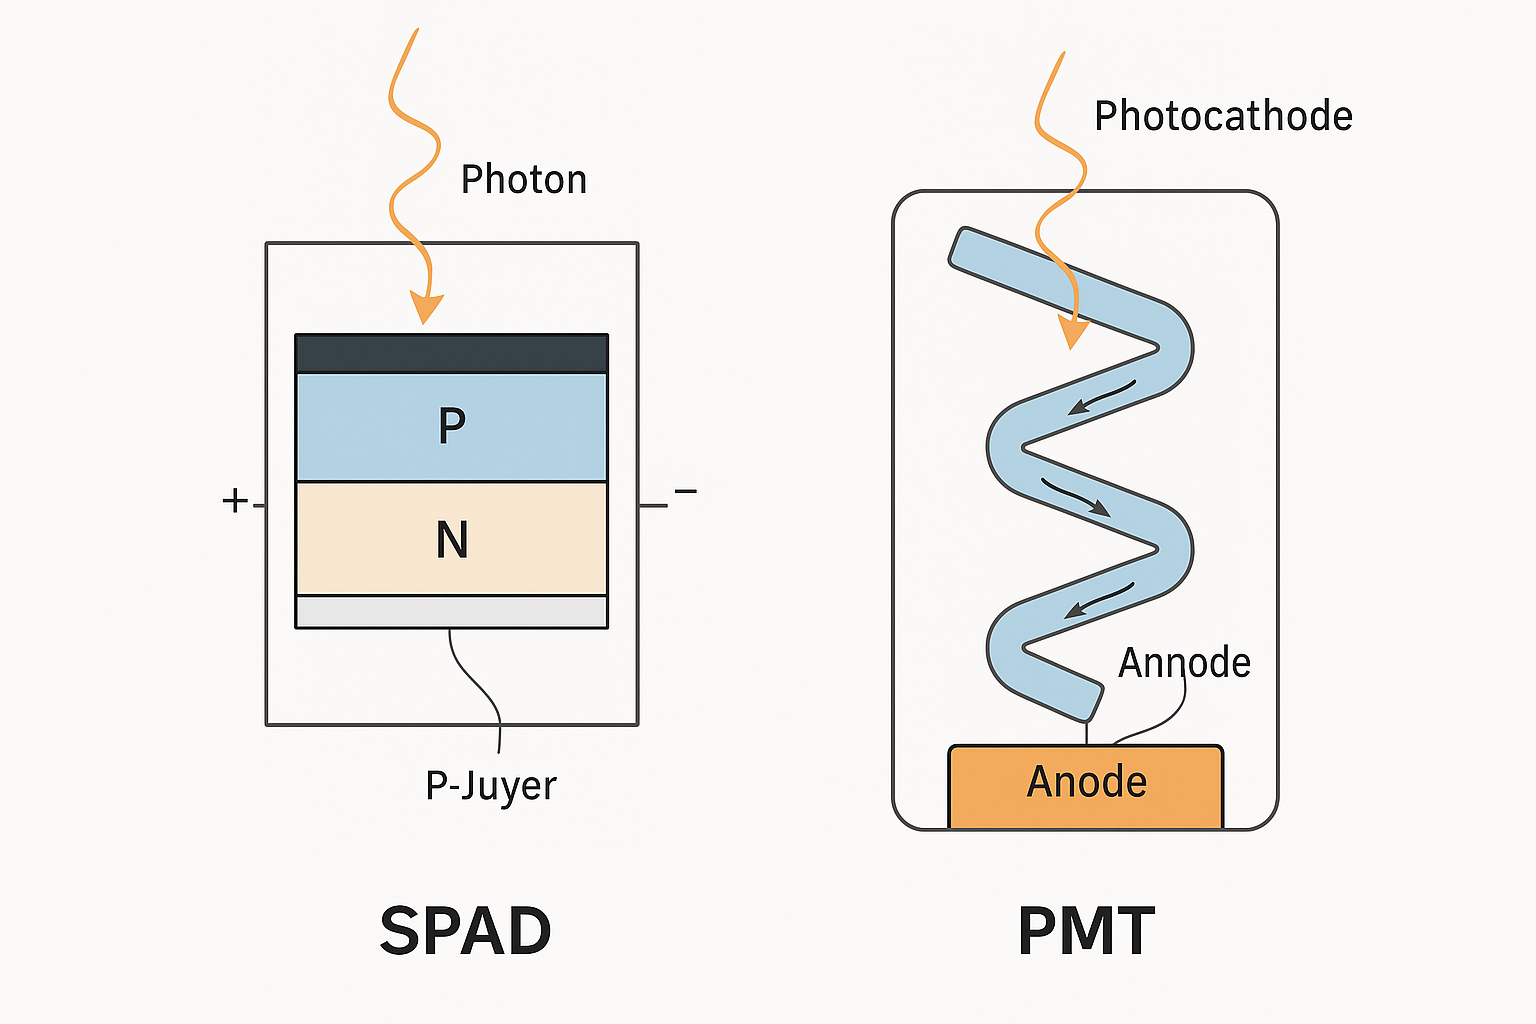
\includegraphics[width=0.9\textwidth]{bilder/SPAD-PMT.png}
	\caption{Schematischer Vergleich eines SPAD (Single-Photon Avalanche Diode, links) und eines PMT (Photomultiplier Tube, rechts). }
	\label{fig:spad_pmt}
\end{figure}
\begin{tcolorbox}[hinweisbox, title=Didaktischer Vergleich: SPAD vs. PMT]
	\label{box:vergleich SPAD}
	\small
	\begin{tabular}{p{0.48\textwidth} | p{0.48\textwidth}}
		\textbf{Single-Photon Avalanche Diode (SPAD)} & \textbf{Photomultiplier Tube (PMT)} \\
		\hline
		Halbleiterbauelement mit speziellem PN-Übergang\index{PN-Übergang}. & Vakuumröhre\index{Vakuumröhre} mit Photokathode und Verstärkungsstufen. \\
		\hline
		Ein Photon erzeugt ein Elektron-Loch-Paar\index{Elektron-Loch-Paar} im Sperrbereich\index{Sperrbereich}. & Ein Photon schlägt ein Elektron aus der Photokathode. \\
		\hline
		Das Elektron löst eine Avalanche-Lawine\index{Avalanche-Lawine} aus – ein elektrischer Impuls entsteht. & Das Elektron wird über mehrere Dynoden beschleunigt und vervielfacht. \\
		\hline
		Sehr hohe Zeitauflösung\index{Zeitauflösung}, ideal für kompakte, integrierte Quantensensoren\index{Quantensensor}. & Hohe Verstärkung, ideal für schwache Lichtquellen (z.\,B. Szintillatoren\index{Szintillator}). \\
		\hline
		Betrieb bei Raumtemperatur\index{Raumtemperatur}, einfache Integration in Chips\index{Chip}. & Benötigt Hochspannung, empfindlich gegen Magnetfelder. \\
		\hline
		Sehr gut geeignet für Arrays und bildgebende Systeme (SiPM). & Klassisch in der Kernphysik\index{Kernphysik}, Astronomie, PET\index{Positronen-Emissions-Tomographie} usw. verwendet. \\
	\end{tabular}
\end{tcolorbox}
\begin{tcolorbox}[didaktikbox, title=Begriffserklärung: Avalanche-Lawine]
	\label{box:avalanche}
	\small
	In einer \textbf{Avalanche-Lawine} (engl. avalanche breakdown) erzeugt ein freies Elektron im starken elektrischen Feld\index{Elektrisches Feld} eines Halbleiters durch Stoßionisation\index{Stoßionisation} weitere Elektronen. Dieser Prozess vervielfacht sich lawinenartig und führt zu einem messbaren Stromimpuls\index{Stromimpuls} – der Nachweis eines einzelnen Photons ist so möglich.
\end{tcolorbox}
\vspace{1em}
\begin{tcolorbox}[didaktikbox, title=Begriffserklärung: Szintillator]
	\label{box:szintillator}
	\small
	Ein \textbf{Szintillator} ist ein Material\index{Material}, das beim Auftreffen ionisierender Teilchen\index{Ionisierendes Teilchen} Licht\index{Licht} emittiert. Dieses sogenannte \emph{Szintillationslicht}\index{Szintillationslicht} kann von Photonendetektoren wie PMTs oder SiPMs registriert werden und ermöglicht die indirekte Messung von Strahlung\index{Strahlung}.
\end{tcolorbox}

%index111
\subsubsection{Einzelphotonenzählung und Quanteneffizienz\index{Einzelphotonenzählung}\index{Quanteneffizienz}}

Die Fähigkeit, \textbf{einzelne Photonen zu detektieren}\index{Photon} ist ein Meilenstein in der Quantentechnologie\index{Quantentechnologie}. Dabei ist nicht nur das „Zählen“ entscheidend, sondern auch die \textbf{Quanteneffizienz}\index{Quanteneffizienz}, also der Anteil der einfallenden Photonen, die tatsächlich ein messbares Signal erzeugen.
\vspace{1em}
\begin{tcolorbox}[physikbox, title=Physikalische Begriffe]
	\label{box:begriffe}
	\small
	\begin{itemize}
		\item \textbf{Einzelphotonenzählung (Single Photon Counting)}: Detektionsmethoden, bei denen jedes registrierte Signal einem einzelnen Photon zugeordnet werden kann.
		\item \textbf{Quanteneffizienz (QE)}: Verhältnis registrierter zu einfallenden Photonen, typischerweise wellenlängenabhängig\index{Wellenlänge}.
	\end{itemize}
\end{tcolorbox}

Technisch kommen dabei meist SPADs\index{SPAD} oder supraleitende Nanodetektoren\index{Supraleitender Nanodetektor} zum Einsatz. Letztere erreichen Quanteneffizienzen nahe 100\%, sind aber kryogen\index{Kryotechnik} zu betreiben.
\newpage
\noindent
\subsubsection*{Wie funktioniert Einzelphotonenzählung?}
\phantomsection
Bei der Einzelphotonenzählung wird jeder einzelne Photonenimpuls als diskretes Ereignis registriert. Der Detektor (z.\,B. ein SPAD) erzeugt bei Eintreffen eines Photons einen elektrischen Impuls – typischerweise eine kurze Spannungs- oder Stromspitze. Diese Impulse werden elektronisch ausgewertet:

\begin{itemize}
	\item Jeder Impuls entspricht einem detektierten Photon.
	\item Ein Zähler\index{Zähler} summiert diese Impulse über definierte Zeitintervalle.
	\item Das Ergebnis ist eine Photonenzahl pro Zeitintervall – z.\,B. „125 Photonen in 1 ms“.
\end{itemize}

Damit dies zuverlässig funktioniert, müssen die Impulse:
\begin{itemize}
	\item eine klare \textbf{Unterschreitungsschwelle} (Schwellwertdetektion\index{Schwellwertdetektion}) überschreiten,
	\item in der Zeit klar voneinander unterscheidbar sein (Totzeit\index{Totzeit} beachten),
	\item und dürfen nicht durch \textbf{thermisches Rauschen}\index{Thermisches Rauschen} oder Dunkelstrom\index{Dunkelstrom} verwechselt werden.
\end{itemize}
\vspace{1em}
\begin{tcolorbox}[didaktikbox, title=Was zählt als Photon? ]
	\label{box:photonenzaehlung}
	\small
	Nicht jeder registrierte Impuls stammt von einem Photon. Detektoren erzeugen auch \emph{Dunkelraten}\index{Dunkelrate} (Fehlsignale ohne Lichteinfall). Hochwertige Einzelphotonendetektoren erreichen jedoch Dunkelraten unter 100 Impulsen pro Sekunde und Quanteneffizienzen über 50–90\,\%.
\end{tcolorbox}

\subsubsection{Anwendungen in Industrie und Grundlagenphysik\index{Anwendungen!Photonendetektion}}

Die Anwendung photonischer Sensorik ist vielfältig:

\begin{itemize}
	\item \textbf{Grundlagenphysik\index{Grundlagenphysik}:} Detektion einzelner Photonen in Quantenoptik\index{Quantenoptik}-Experimenten (z.\,B. Antibunching\index{Antibunching}, HOM-Effekt\index{Hong-Ou-Mandel-Effekt}), Teilchendetektion in der Hochenergiephysik\index{Hochenergiephysik}, astronomische Beobachtungen\index{Astronomie} (z.\,B. Hubble\index{Hubble-Teleskop}, JWST\index{James-Webb-Weltraumteleskop}).
	\item \textbf{Industrielle Anwendungen\index{Industrie}:} Qualitätskontrolle\index{Qualitätskontrolle}, Laserscanner\index{Laserscanner}, Lichtvorhänge\index{Lichtvorhang}, Positionssensoren\index{Positionssensor}, Photonenspektroskopie\index{Photonenspektroskopie}.
	\item \textbf{Medizin und Biowissenschaften\index{Medizin}:} Fluoreszenzmikroskopie\index{Fluoreszenzmikroskopie}, PET-Scanner\index{Positronen-Emissions-Tomographie}, optische Tomographie\index{Optische Tomographie}.
\end{itemize}

\begin{tcolorbox}[hinweisbox, title=Hinweis zur Bedeutung der Detektionstechnologie]
	\label{box:detektionstechnologie}
	Die kontinuierliche Verbesserung der Photonen-Detektion ist eine Voraussetzung für den Fortschritt in der Quantenkommunikation\index{Quantenkommunikation}, der medizinischen Bildgebung\index{Medizinische Bildgebung} und der Grundlagenforschung\index{Grundlagenforschung}. Viele Entwicklungen der Quantentechnologie hängen direkt von der Fähigkeit ab, Photonen präzise und verlustarm nachzuweisen.
\end{tcolorbox}

\subsection{Photonen in der medizinischen Bildgebung\index{Photonen in der medizinischen Bildgebung}}

Photonen spielen eine zentrale Rolle in vielen bildgebenden Verfahren der modernen Medizin. Dabei reicht ihr Einsatzspektrum von hochenergetischer Röntgenstrahlung\index{Röntgenstrahlung} bis hin zu sanftem, sichtbarem Laserlicht\index{Laserlicht} in der optischen Diagnostik\index{Optische Diagnostik}. Unterschiedliche physikalische Prozesse – Absorption\index{Absorption}, Streuung\index{Streuung}, Fluoreszenz\index{Fluoreszenz} oder Emission\index{Emission} – werden genutzt, um Kontrast im Gewebe sichtbar zu machen oder pathologische Strukturen zu identifizieren.

%index
\subsubsection{Röntgen, CT und PET}

\textbf{Röntgenstrahlung}\index{Röntgenstrahlung} basiert auf hochenergetischen Photonen, die durch Absorption und Abschwächung beim Durchtritt durch den Körper ein Bild erzeugen. Dichteres Gewebe (z.\,B. Knochen) absorbiert mehr Photonen und erscheint heller auf dem Detektor.

\textbf{Computertomographie (CT)}\index{Computertomographie (CT)} erweitert diese Technik, indem sie aus vielen Röntgenprojektionen ein 3D-Bild rekonstruiert. Hierfür werden rotierende Röntgenquellen und Detektorarrays verwendet.

\textbf{Positronen-Emissions-Tomographie (PET)}\index{Positronen-Emissions-Tomographie (PET)} nutzt einen anderen Mechanismus: Radiopharmaka\index{Radiopharmakon} emittieren Positronen\index{Positron}, die mit Elektronen\index{Elektron} annihilieren – dabei entstehen zwei Photonen mit einer Energie von \SI{511}{keV}, die in entgegengesetzten Richtungen ausgesendet und durch Ringdetektoren erfasst werden. Aus der Koinzidenz der Detektion wird der Ursprungsort rekonstruiert.
\vspace{1em}
\begin{tcolorbox}[physikbox, title=Photonen bei der PET]
	\label{box:PET}
	\small
	Bei der PET entstehen zwei Gamma-Photonen mit \SI{511}{keV} bei der Annihilation von Elektron und Positron. Diese Photonen verlassen den Körper fast ungehindert und ermöglichen eine präzise Lokalisation des Stoffwechsels – z.\,B. bei Tumoren.
\end{tcolorbox}
\begin{figure}[H]
	\centering
	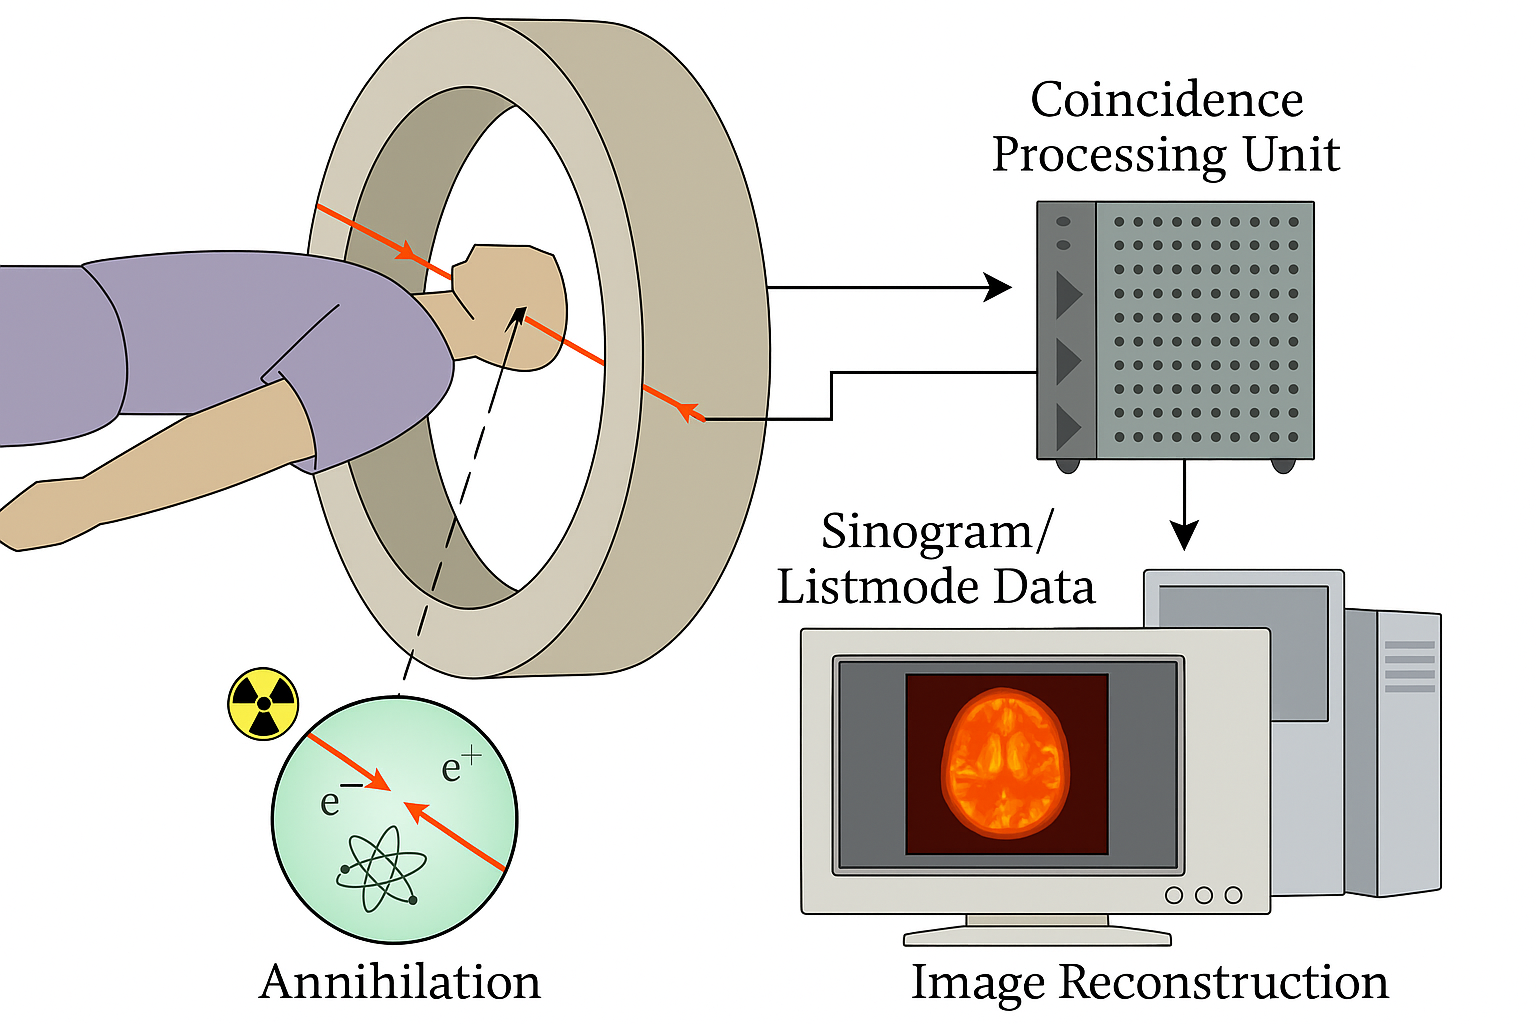
\includegraphics[width=0.85\textwidth]{bilder/petscan.png}
	\caption{Prinzip der Positronen-Emissions-Tomographie (PET): Ein verabreichtes Radiopharmakon emittiert ein Positron, das mit einem Elektron annihiliert. Dabei entstehen zwei Gamma-Photonen mit je \SI{511}{keV}, die in entgegengesetzten Richtungen ausgesendet und von Detektoren im PET-Ring registriert werden. Aus der Koinzidenz der Signale wird der Ursprungsort rekonstruiert.}
	\label{fig:pet_prinzip}
\end{figure}
\begin{tcolorbox}[didaktikbox, title=Begriffserklärung: Annihilation]
	\label{box:annihilation}
	\small
	Bei der \textbf{Annihilation} treffen ein Teilchen und sein Antiteilchen aufeinander und vernichten sich. Ihre Masse wird vollständig in Energie umgewandelt – meist in Form von Photonen. In der PET entsteht bei der Annihilation eines Elektrons mit einem Positron ein Photon-Paar mit je \SI{511}{keV}.
\end{tcolorbox}
\vspace{1em}
\begin{tcolorbox}[didaktikbox, title=Begriffserklärung: Radiopharmakon]
	\label{box:radiopharmakon}
	\small
	Ein \textbf{Radiopharmakon} ist ein radioaktiv markierter Wirkstoff, der gezielt in den Körper eingebracht wird. In der PET wird z.\,B. [\textsuperscript{18}F]FDG verwendet – eine Zucker-ähnliche Substanz, die sich in stoffwechselaktiven Geweben (wie Tumoren) anreichert. Die dort entstehenden Positronen liefern durch Annihilation das Bildsignal.
\end{tcolorbox}

\subsubsection{Optische Tomographie und Fluoreszenzbildgebung}

Im Gegensatz zur ionisierenden Strahlung setzen diese Verfahren auf sichtbares oder nahinfrarotes Licht.

\textbf{Diffuse optische Tomographie (DOT)}\index{Diffuse optische Tomographie (DOT)} verwendet Lichtquellen und Detektoren auf der Hautoberfläche. Die Photonen durchdringen das Gewebe, werden gestreut und absorbiert. Aus der Lichtverteilung kann auf die optischen Eigenschaften im Inneren geschlossen werden.

\textbf{Fluoreszenzbildgebung}\index{Fluoreszenzbildgebung} nutzt Substanzen (Fluorophore\index{Fluorophor}), die durch Licht angeregt werden und in einer anderen Wellenlänge wieder emittieren. Diese Methode erlaubt z.\,B. die Darstellung molekularer Prozesse oder Tumormarker.
\vspace{1em}
\begin{tcolorbox}[didaktikbox, title=Vorteil optischer Verfahren]
	\label{box:optisches Verfahren}
	\small
	Optische Methoden sind nicht-invasiv, strahlungsfrei und eignen sich besonders für Oberflächen- und funktionelle Bildgebung – z.\,B. bei Säuglingen, in der Neurodiagnostik oder der molekularen Bildgebung.
\end{tcolorbox}

\subsubsection{Laser in der Chirurgie und Diagnostik}

Laser\index{Laser} werden sowohl zur \textbf{Bildgebung} als auch zur \textbf{Gewebeeinwirkung} eingesetzt:

\begin{itemize}
	\item \textbf{Diagnostisch:} Konfokale Laser-Scanning-Mikroskopie\index{Konfokale Laser-Scanning-Mikroskopie}, optische Kohärenztomographie (OCT)\index{Optische Kohärenztomographie (OCT)}, Spektroskopie\index{Spektroskopie}.
	\item \textbf{Chirurgisch:} Gewebeschnitt, Koagulation, Ablation – je nach Wellenlänge, Pulsdauer und Leistung.
\end{itemize}
\newpage
\noindent
Laserchirurgie\index{Laserchirurgie} nutzt die präzise Fokussierung von Photonen zur gezielten Gewebeeinwirkung ohne mechanische Belastung. Typische Anwendungen sind:

\begin{itemize}
	\item Augenheilkunde\index{Augenheilkunde} (z.\,B. LASIK\index{LASIK}),
	\item Dermatologie\index{Dermatologie} (z.\,B. Tattoo-Entfernung\index{Tattoo-Entfernung}),
	\item Tumorchirurgie\index{Tumorchirurgie} (präzise Schnitte mit minimalem Blutverlust).
\end{itemize}

\begin{tcolorbox}[hinweisbox, title=Laserparameter]
	\label{box:laserparameter}
	\small
	Die Wirkung eines Lasers hängt stark von seiner Wellenlänge, Pulsdauer, Energie und Fokussierung ab. Kurze Pulse mit hoher Leistung ermöglichen präzise Schnitte, ohne umliegendes Gewebe zu beschädigen.
\end{tcolorbox}

\begin{figure}[H]
	\centering
	\includegraphics[width=0.85\textwidth]{bilder/oct.png}
	\caption{Schematische Darstellung der optischen Kohärenztomographie (OCT): Licht einer breitbandigen Quelle wird durch einen Strahlteiler aufgeteilt. Ein Teil trifft auf einen beweglichen Referenzspiegel (Referenzarm), der andere auf das zu untersuchende Gewebe (Sample). Die reflektierten Lichtanteile interferieren, und aus den Interferenzmustern wird das Tiefenprofil rekonstruiert. Das Ergebnis ist ein hochauflösendes Bild, z.\,B. der Netzhaut.}
	\label{fig:oct_prinzip}
\end{figure}

\begin{tcolorbox}[didaktikbox, title=Didaktische Erläuterung: Interferenz in der OCT]
	\label{box:interferenz_oct}
	\small
	\textbf{Interferenz} entsteht, wenn zwei Lichtwellen überlagert werden – je nach Phasenlage verstärken oder löschen sie sich aus. In der OCT wird diese Eigenschaft genutzt, um die Position reflektierender Strukturen im Gewebe mit hoher Präzision zu bestimmen.
	
	Nur wenn die optischen Weglängen im \emph{Sample Arm} und im \emph{Reference Arm} nahezu gleich sind, kommt es zu einem Interferenzsignal. Aus der gemessenen Intensität als Funktion der Referenzarm-Position ergibt sich ein sogenannter \textbf{A-Scan} – ein Tiefenprofil entlang einer Linie im Gewebe.
	
	Durch seitliches Verschieben des Messstrahls entsteht eine Vielzahl an A-Scans nebeneinander, die zu einem \textbf{B-Scan} (2D-Querschnitt) zusammengesetzt werden. So entsteht ein detailliertes Bild des untersuchten Gewebes – z.\,B. der Netzhaut.
\end{tcolorbox}

%index
\subsection{Photonen in der Kommunikation}
\index{Photonen in der Kommunikation}
\index{Datenübertragung}
\index{Quantenkommunikation}

Photonen bilden das Rückgrat moderner Datenübertragung – sowohl in klassischen Glasfasernetzen als auch in zukünftigen quantenbasierten Systemen. Die verlustarme Ausbreitung von Licht in optischen Medien, kombiniert mit hohen Bandbreiten und geringen Latenzen, macht die photonische Kommunikationstechnologie zu einem entscheidenden Faktor in der globalen Informationsinfrastruktur.

\subsubsection{Glasfaser und optische Netzwerke}
\index{Glasfaser}
\index{Optische Netzwerke}
\index{Totalreflexion}
\index{Wellenlängenmultiplexing}
\index{DWDM}
\index{EDFA}

\textbf{Glasfasern} leiten Licht durch Totalreflexion in einem dünnen Quarzfaserkern. Dabei können Photonen über Strecken von mehreren hundert Kilometern mit minimaler Dämpfung übertragen werden.

Vorteile:
\begin{itemize}
	\item extrem hohe Datenraten (Terabit/s),
	\item keine elektromagnetische Störung,
	\item geringe Dämpfung (z.\,B. \SI{0.2}{dB/km} bei \SI{1550}{nm}).
\end{itemize}

\textbf{Optische Netzwerke} nutzen Wellenlängenmultiplexing (DWDM), Verstärker (EDFA) und modulierte Lasersysteme, um große Datenmengen parallel und effizient zu übertragen – von Backbone-Netzen bis hin zu Glasfaseranschlüssen im Haus.
\vspace{1em}
\begin{tcolorbox}[physikbox, title=Totalreflexion in Glasfasern]
	\label{box:glasfaser}
	\small
	Die Lichtführung in einer Glasfaser erfolgt durch Totalreflexion an der Grenzfläche zwischen dem höherbrechenden Kern und dem Mantelmaterial. Der kritische Winkel bestimmt, ob das Licht innerhalb des Kerns „gefangen“ bleibt.
\end{tcolorbox}
\begin{figure}[H]
	\centering
	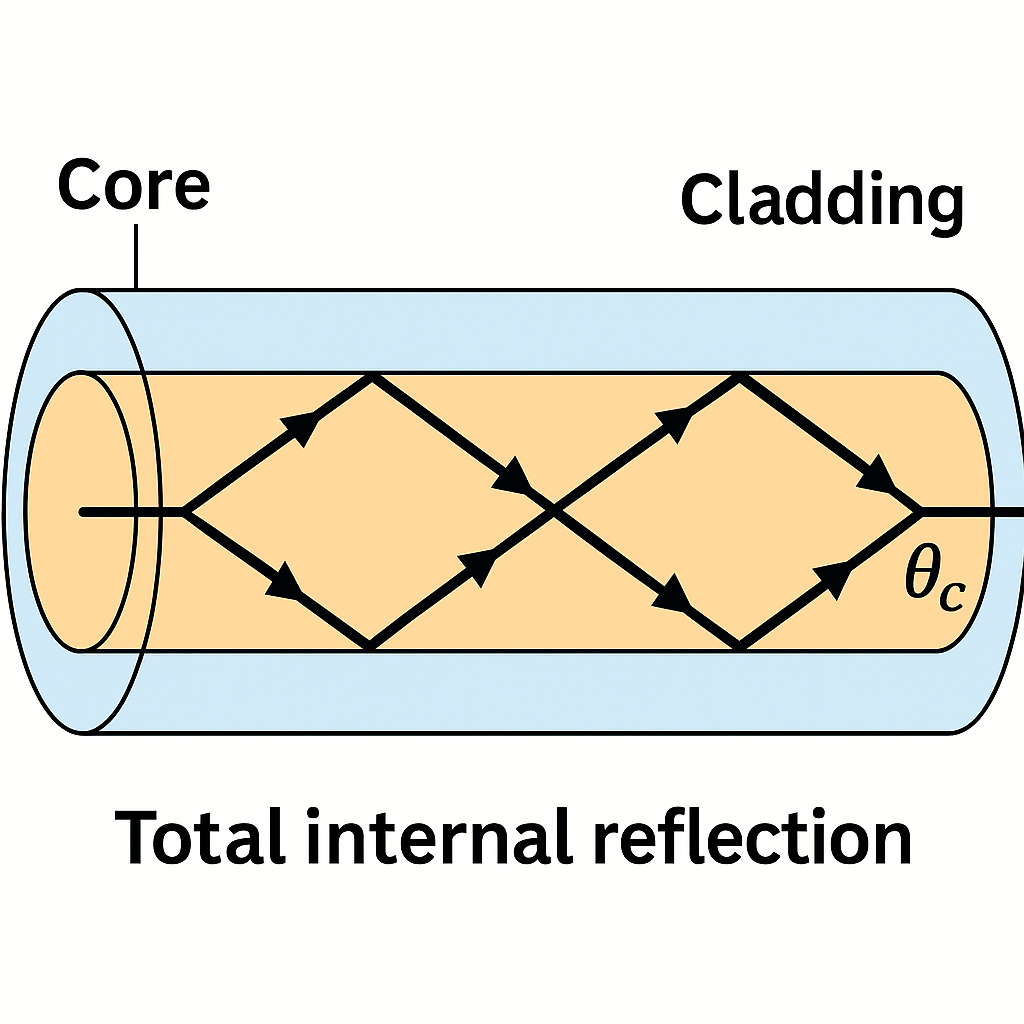
\includegraphics[width=0.8\textwidth]{bilder/glasfaser.png}
	\caption{Schematische Darstellung der Totalreflexion in einer Glasfaser: Das Licht (Photonen) wird im höherbrechenden Kern geführt und an der Grenzfläche zum Mantel (Cladding) vollständig reflektiert. So bleibt das Licht auch über große Strecken im Kern „gefangen“.}
	\label{fig:totalreflexion}
\end{figure}

%index
\subsubsection{Quantenkommunikation und QKD}\index{Quantenkommunikation}\index{QKD}\index{Photonen!Quantenkommunikation}\index{Polarisation!Photonen}\index{Verschränkung!Photonen}

Die \textbf{Quantenkommunikation} nutzt quantenmechanische Zustände von Photonen – etwa Polarisation oder Verschränkung –, um Informationen absolut abhörsicher zu übertragen.

\textbf{QKD (Quantum Key Distribution)} ist eine praktische Anwendung: Zwei Parteien (Alice und Bob) tauschen einen geheimen Schlüssel aus. Jeder Abhörversuch (Eve) verändert unweigerlich den Quantenzustand der Photonen und wird dadurch erkennbar.

\begin{tcolorbox}[didaktikbox, title=Was macht QKD sicher?] \index{QKD!Sicherheit}
	\label{box:qkd}
	\small
	Die Sicherheit beruht auf zwei quantenphysikalischen Prinzipien:
	\begin{itemize}
		\item \textbf{Nicht-Klonbarkeit}: Unbekannte Quantenzustände können nicht exakt kopiert werden.
		\item \textbf{Messstörung}: Jede Messung beeinflusst den Zustand – ein Abhörversuch stört das System messbar.
	\end{itemize}
\end{tcolorbox}

\textbf{BB84} ist das erste und bekannteste QKD-Protokoll. Es nutzt zufällige Polarisationen und Basiswechsel zur Erzeugung eines Schlüssels, der anschließend über einen klassischen Kanal verifiziert wird.

\vspace{1em}
\begin{tcolorbox}[didaktikbox, title=Wie funktioniert QKD (z.\,B. BB84)?] \index{QKD!BB84}\index{Quantenkommunikation!BB84}
	\label{box:wie funktioniert QKD}
	\small
	Beim BB84-Protokoll sendet Alice einzelne Photonen, deren Polarisation zufällig gewählt ist – z.\,B. horizontal ($\rightarrow$), vertikal ($\uparrow$), diagonal ($\searrow$) oder antidiagonal ($\nwarrow$). Bob misst ebenfalls in zufälligen Basen.
	
	Nur wenn Sender- und Empfängerbasis übereinstimmen, ergibt sich ein valides Bit. Nach dem Austausch vergleichen Alice und Bob (öffentlich) die verwendeten Basen und behalten nur die passenden. Aus diesen Bits entsteht der Schlüssel.
	
	Wird ein Photon abgehört, ändert sich seine Polarisation – dadurch erkennen Alice und Bob Störungen im Schlüssel und können Abhörversuche entdecken.
\end{tcolorbox}

%index
\subsubsection{Photonische Chips und zukünftige Systeme}\index{Photonische Chips}\index{Siliziumphotonik}\index{Photonen!Photonische Chips}\index{Datenverarbeitung!photonisch}\index{Logiksysteme!photonische}

Mit dem Aufkommen von \textbf{photonischen Chips} werden Lichtsignale nicht mehr durch Glasfasern allein, sondern direkt durch integrierte optische Schaltkreise geleitet. Diese ermöglichen:

\begin{itemize}
	\item kompakte, energieeffiziente Datenverarbeitung,
	\item lichtbasierte Logik- und Modulationssysteme,
	\item neue Konzepte für neuronale Netze und KI-Beschleuniger.
\end{itemize}

Photonische Chips kombinieren Laser, Modulatoren, Wellenleiter und Detektoren auf einem einzigen Substrat – oft Siliziumphotonik.

\begin{tcolorbox}[hinweisbox, title=Zukunft der photonischen Kommunikation] \index{Photonenbasierte Kommunikation}
	\label{box:Zukunft Kommunikation}
	\small
	Photonenbasierte Kommunikation ist nicht nur schneller als klassische Elektronik – sie wird zur Voraussetzung für sichere Quantennetzwerke, lichtbasierte Prozessoren und globale, abhörsichere Kommunikation.
\end{tcolorbox}

\subsection{Photonen in der astronomischen Beobachtung}\index{Astronomie!Photonen}\index{Photonen!Astronomie}\index{Photonen!astronomische Beobachtung}

Die Beobachtung von Photonen aus dem All ist das Fundament der modernen Astronomie. Da Photonen – anders als etwa Gravitationswellen oder Neutrinos – vergleichsweise leicht messbar sind, liefern sie einen Großteil unserer Informationen über das Universum. Ob sichtbares Licht, Radiostrahlung oder hochenergetische Gammastrahlen – jedes Photon, das die Erde erreicht, enthält eine Botschaft aus Raum und Zeit.

\subsubsection{Detektion von Photonen aus dem All}\index{Detektion!Photonen}\index{Photonen!Detektion!astronomisch}

Teleskope und Detektoren auf der Erde und im Weltall messen Photonen verschiedenster Wellenlängenbereiche:

\begin{itemize}
	\item \textbf{Optischer Bereich:} CCDs (Charge-Coupled Devices), CMOS-Sensoren
	\item \textbf{Infrarot und Radio:} Bolometer, Radioteleskope
	\item \textbf{Röntgen und Gamma:} Weltraumteleskope mit Szintillatoren und Halbleiterdetektoren
\end{itemize}

Die Analyse dieser Photonen liefert Informationen über Temperatur, Bewegung (Dopplerverschiebung), Zusammensetzung und Entfernung kosmischer Objekte.

\vspace{1em}
\begin{tcolorbox}[physikbox, title=Warum kommen manche Photonen nicht auf der Erde an?] \index{Erdatmosphäre!Photonenabsorption}\index{Photonen!Erdatmosphäre}
	\label{box:photonen auf erde}
	\small
	Die Erdatmosphäre ist für viele Wellenlängenbereiche nicht durchlässig – insbesondere für UV-, Röntgen- und Gammastrahlen. Deshalb müssen entsprechende Teleskope außerhalb der Atmosphäre – z.\,B. im Erdorbit – positioniert werden.
\end{tcolorbox}

%index
\subsubsection{Adaptive Optik, Spektroskopie und Teleskope}
\index{Adaptive Optik}
\index{Spektroskopie}
\index{Teleskope}
\index{Interferometrie}

\textbf{Teleskope} sammeln Photonen\index{Photon} und fokussieren sie auf Detektoren. Moderne Großteleskope (z.\,B. das VLT\index{Very Large Telescope (VLT)} oder ELT\index{Extremely Large Telescope (ELT)}) nutzen adaptive Optik, um die Bildqualität zu verbessern:

- \textbf{Adaptive Optik} kompensiert atmosphärische Störungen in Echtzeit durch deformierbare Spiegel.
- \textbf{Spektroskopie} zerlegt das Licht in seine Wellenlängen und erlaubt die Analyse chemischer Zusammensetzung, Temperatur und Bewegung von Himmelskörpern.
- \textbf{Interferometrie} kombiniert mehrere Teleskope zu einem virtuellen Riesenteleskop mit extrem hoher Winkelauflösung.
\begin{figure}[H]
	\centering
	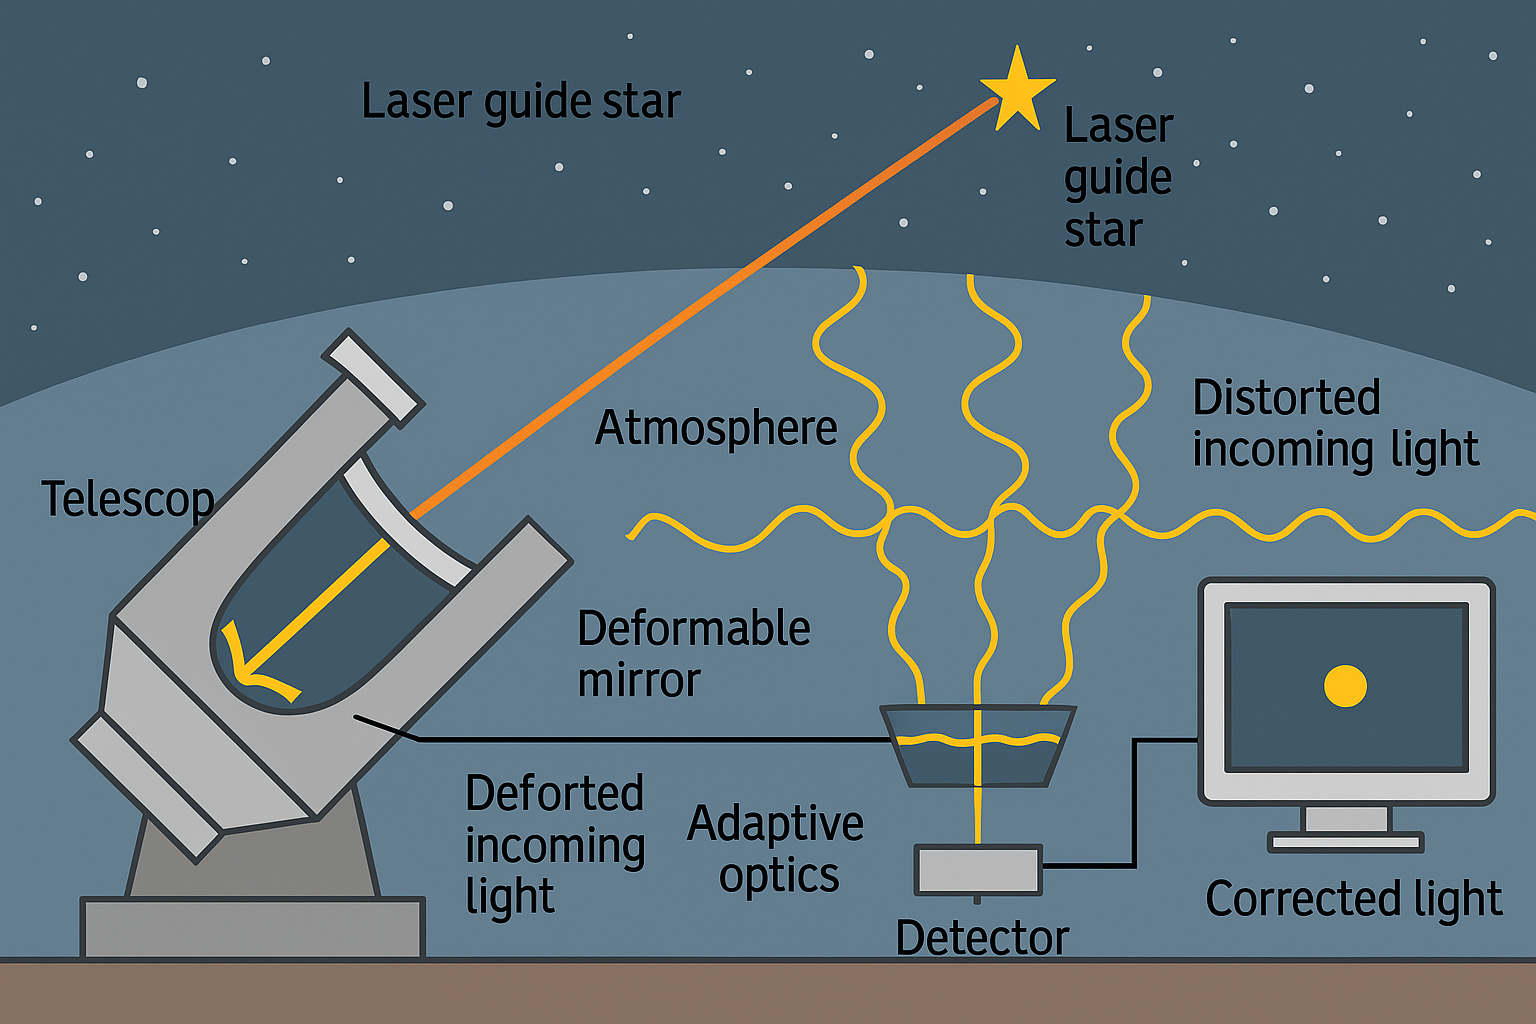
\includegraphics[width=0.9\textwidth]{bilder/Teleskop.png}
	\caption{Schematische Darstellung eines Teleskops mit adaptiver Optik. Ein Wellenfrontsensor analysiert Verzerrungen durch die Atmosphäre. Eine deformierbare Spiegeloberfläche korrigiert diese in Echtzeit, sodass ein scharfes Bild entsteht.}
	\label{fig:adaptive_optik}
\end{figure}

\begin{tcolorbox}[didaktikbox, title=Was zeigt ein Spektrum?]
	\label{box:was zeigt spektrum}
	\small
	Ein Spektrum\index{Spektrum} ist die Verteilung der Intensität der Photonen nach Wellenlängen. Typische Merkmale sind:
	\begin{itemize}
		\item \textbf{Emissionslinien}\index{Emissionslinien} $\rightarrow$ heiße, strahlende Gase,
		\item \textbf{Absorptionslinien}\index{Absorptionslinien} $\rightarrow$  kalte Gase vor heißen Quellen,
		\item \textbf{Rotverschiebung}\index{Rotverschiebung} $\rightarrow$  Bewegung des Objekts vom Beobachter weg.
	\end{itemize}
\end{tcolorbox}
\begin{figure}[H]
	\centering
	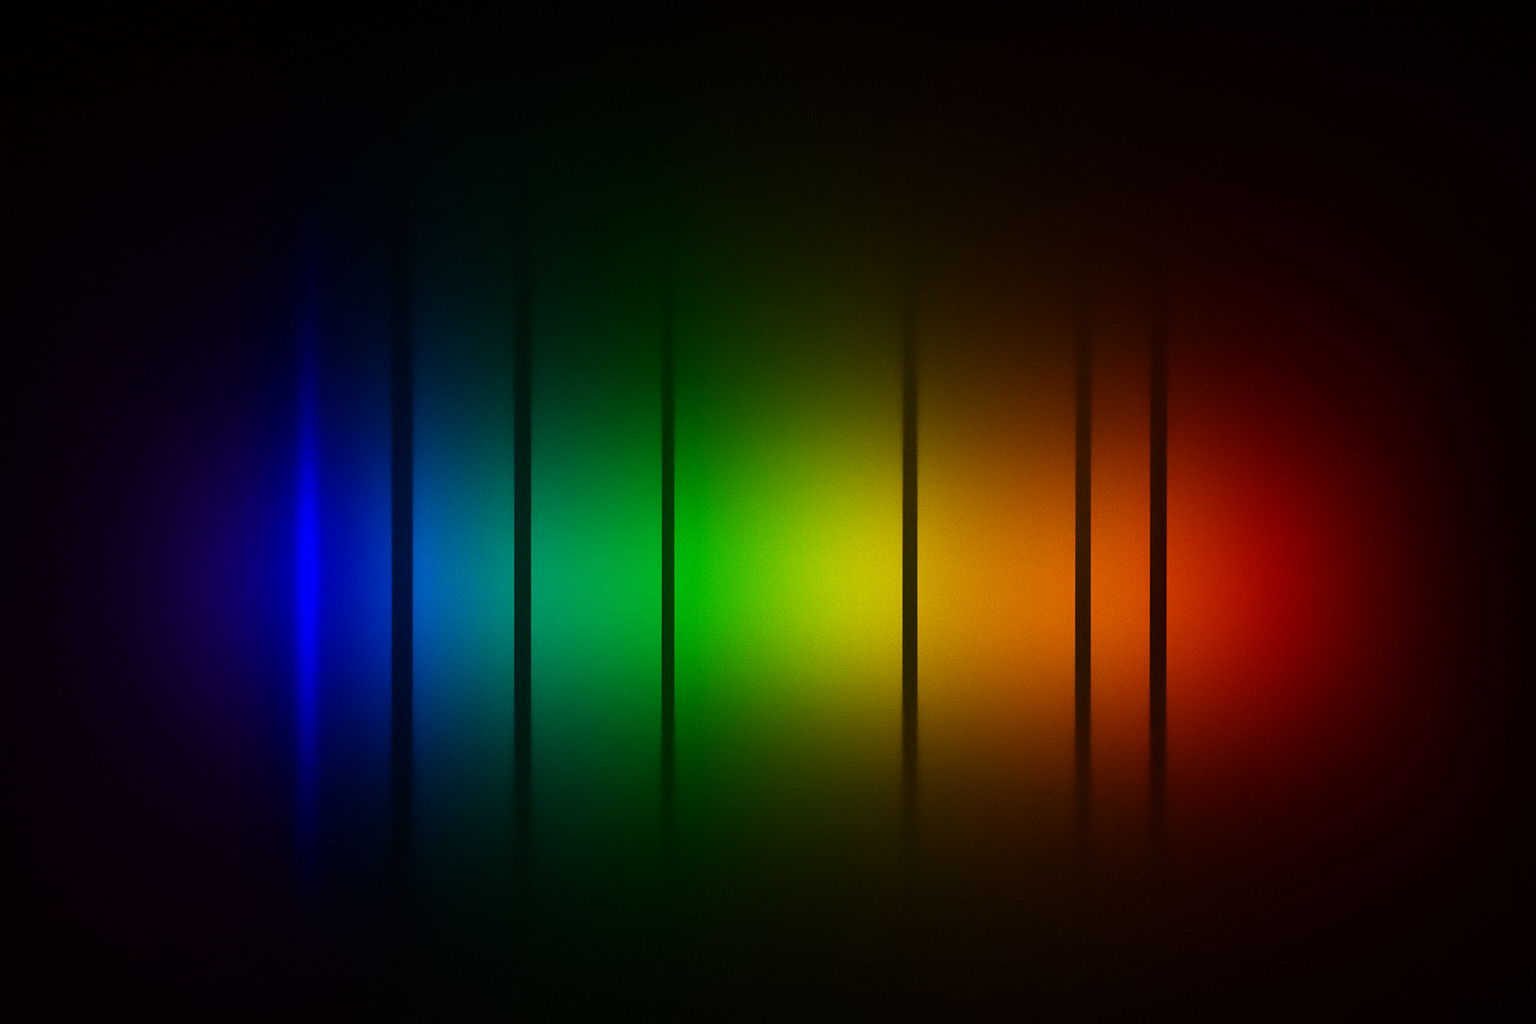
\includegraphics[width=0.9\textwidth]{bilder/emissionslinien.png}
	\caption{Emission von Strahlungslinien eines glühenden \newline Wasserstoffgases.}
	\label{fig:emission_hydrogen}
\end{figure}

\begin{tcolorbox}[physikbox, title=Spektrallinien und Rotverschiebung]
	\label{box:spektrallinien}
	\small
	\begin{itemize}
		\item \textbf{Emissionslinien} entstehen, wenn Atome spezifische Photonen aussenden. Diese Linien sind hell und charakteristisch für das jeweilige Element\index{Elementspektrum}.
		\item \textbf{Absorptionslinien} entstehen, wenn Photonen bestimmter Frequenzen von einem durchstrahlten Gas absorbiert werden – sie fehlen dann im Spektrum.
		\item \textbf{Rotverschiebung:} Entfernt sich eine Lichtquelle, verschieben sich alle Linien zu längeren Wellenlängen – in Richtung Rot. Dies wird zur Messung kosmischer Bewegungen\index{Kosmische Expansion} genutzt.
	\end{itemize}
\end{tcolorbox}

%index
\subsubsection{Photonen in der Gravitationswellenastronomie}
\index{Gravitationswellenastronomie}
\index{Gravitationswellen}
\index{Photon}
\index{Interferometer}
\index{LIGO}
\index{Virgo}

Gravitationswellen sind fundamentale Verzerrungen der Raumzeit\index{Raumzeit} – ausgelöst durch beschleunigte Massen, etwa bei der Verschmelzung Schwarzer Löcher\index{Schwarzes Loch}. Sie sind keine elektromagnetischen Wellen und bestehen nicht aus Photonen. Dennoch sind es gerade Photonen, die den Nachweis dieser Phänomene ermöglichen: als präzise Messsonden in hochsensitiven Interferometern.

\vspace{0.5em}
\textbf{LIGO, Virgo und andere Gravitationswellen-Detektoren} nutzen kilometerlange Laserinterferometer, um winzige Veränderungen der Raumzeit zu messen. Dabei werden Laserstrahlen (bestehend aus kohärenten Photonen) in zwei senkrecht zueinander verlaufende Arme gesendet, an Spiegeln reflektiert und am Ausgang überlagert. Eine vorbeiziehende Gravitationswelle verändert minimal die Armlängen – und damit das Interferenzmuster.

\vspace{1em}
\begin{tcolorbox}[physikbox, title=Photonen als Messwerkzeug für Raumkrümmung]
	\label{box:messwerkzeug}
	\small
	Laserinterferometer wie LIGO nutzen Photonen, um Differenzen in der Armlänge von bis zu \SI{1e-19}{m} zu detektieren – das ist etwa tausendmal kleiner als ein Proton\index{Proton}. Der Zeitunterschied, den ein Photon auf zwei Wegen durch das Interferometer benötigt, ändert sich messbar durch eine vorbeiziehende Gravitationswelle.
\end{tcolorbox}

Diese Technik beruht auf der Interferenz\index{Interferenz} kohärenter Lichtwellen. Sobald die beiden Teilstrahlen nach ihrem Lauf durch die beiden Arme wieder zusammengeführt werden, kommt es – je nach Phasenverschiebung – zu konstruktiver oder destruktiver Interferenz. Schon kleinste Änderungen der optischen Weglängen beeinflussen dieses Muster. Auf diese Weise lassen sich selbst winzige Krümmungen der Raumzeit nachweisen.

\vspace{0.5em}
Dank dieser photonengestützten Präzisionsmessung wurden erstmals Ereignisse wie die Verschmelzung Schwarzer Löcher, die Kollision von Neutronensternen\index{Neutronenstern} oder Spuren des kosmischen Gravitationshintergrunds\index{Kosmischer Gravitationshintergrund} experimentell nachgewiesen. Photonen machen also sichtbar, was ansonsten jenseits direkter Beobachtung läge – ein weiterer Beleg für ihre zentrale Rolle in der modernen Physik.

\vspace{1em}
\begin{tcolorbox}[didaktikbox, title=Wie funktioniert ein Interferometer? \label{box:interferometer}]
	\small
	Ein Interferometer nutzt das Prinzip der Überlagerung (Interferenz) von Lichtwellen, um kleinste Längenunterschiede sichtbar zu machen. 
	
	\begin{itemize}
		\item Ein Laserstrahl\index{Laser} wird mithilfe eines Strahlteilers in zwei Teilstrahlen aufgespalten.
		\item Diese laufen entlang zweier rechtwinklig zueinander stehender Arme zu Spiegeln, werden reflektiert und wieder zusammengeführt.
		\item Wenn sich die optischen Weglängen der beiden Arme genau entsprechen, löschen sich die Wellen teilweise oder vollständig aus – das Interferenzmuster ist konstant.
		\item Verändert sich eine Armlänge minimal (z.\,B. durch eine Gravitationswelle), verschiebt sich die Phase einer Welle, und das Interferenzmuster ändert sich messbar.
	\end{itemize}
	
	So können selbst winzige Längenänderungen – kleiner als ein Atomdurchmesser – durch die Analyse der Lichtintensität am Detektor erkannt werden. Das Licht dient dabei als präzise „Messlatte“ im Raum.
\end{tcolorbox}

\vspace{1em}
\begin{tcolorbox}[didaktikbox, title=Warum sind Photonen so genau messbar? \label{box:photonen_genau}]
	\small
	Photonen sind ideale Messwerkzeuge – aus mehreren Gründen:
	
	\begin{itemize}
		\item \textbf{Hohe Kohärenz:} Laserlicht besteht aus kohärenten Photonen – also Wellen mit exakt gleicher Frequenz und stabiler Phasenlage. Das ermöglicht extrem empfindliche Interferenzeffekte.
		\item \textbf{Geringe Wechselwirkung:} Photonen wechselwirken kaum mit Materie. Dadurch lassen sich lange Laufstrecken realisieren, ohne dass sie gestört oder abgelenkt werden.
		\item \textbf{Quantennatur:} Einzelne Photonen sind diskrete Quantenobjekte\index{Quantennatur}. Ihre Erfassung erzeugt eindeutige, zählbare Signale – ideal für präzise Zeit- oder Ortsmessungen.
		\item \textbf{Lichtgeschwindigkeit als Konstante:} Die Geschwindigkeit von Photonen im Vakuum ist konstant\index{Lichtgeschwindigkeit}. Dadurch eignen sie sich als natürliche „Zeit- und Längenmaßstäbe“.
	\end{itemize}
	
	Diese Eigenschaften machen Photonen unverzichtbar in der modernen Messtechnik – vom Interferometer über Quantensensoren\index{Quantensensor} bis hin zu optischen Atomuhren\index{Optische Atomuhr}.
\end{tcolorbox}

\subsubsection{Fazit}

Photonen sind nicht nur zentrale Objekte der modernen Physik, sondern auch unverzichtbare Werkzeuge in Wissenschaft, Technik, Medizin und Kommunikation. Dieses Kapitel hat gezeigt, wie vielfältig und präzise Photonen kontrolliert, erzeugt und detektiert werden können:

\begin{itemize}
	\item In der \textbf{Lasertechnologie}\index{Lasertechnologie} ermöglichen stimulierte Emission und kohärente Lichtverstärkung Anwendungen von der Materialbearbeitung bis zur Quantenoptik\index{Quantenoptik}.
	\item \textbf{Photonendetektoren}\index{Photonendetektor} wie SPADs\index{SPAD} oder PMTs\index{Photomultiplier (PMT)} erlauben die Einzelphotonenzählung mit hoher Quanteneffizienz\index{Quanteneffizienz} – Grundlage für Quantentechnologien\index{Quantentechnologie} und präzise Bildgebung.
	\item In der \textbf{medizinischen Diagnostik}\index{Medizinische Diagnostik} werden Photonen zur Bildgebung mit hoher räumlicher Auflösung und minimaler Belastung eingesetzt – vom Röntgen\index{Röntgen} bis zur Fluoreszenzmikroskopie\index{Fluoreszenzmikroskopie}.
	\item Die \textbf{optische Kommunikation}\index{Optische Kommunikation} nutzt Photonen zur schnellen, verlustarmen und abhörsicheren Datenübertragung – in Glasfasern\index{Glasfaser} wie auch in Quantenkommunikationssystemen\index{Quantenkommunikation}.
	\item In der \textbf{astronomischen Beobachtung}\index{Astronomie} liefern Photonen entscheidende Informationen über Struktur, Bewegung und Zusammensetzung des Universums – bis hin zum Nachweis von Gravitationswellen durch interferometrische Messung.
\end{itemize}

Die Fähigkeit, einzelne Photonen gezielt zu erzeugen, zu lenken und zu messen, markiert einen technologischen Wendepunkt: Von klassischen Anwendungen bis zur Quanteninformationstechnik\index{Quanteninformationstechnik} eröffnet das Photon neue Horizonte – in Forschung, Industrie und Gesellschaft.




	\chapter{Photonen und die Zukunft der Physik}
\setcounter{section}{7}
\setcounter{subsection}{0}
\setcounter{subsubsection}{1}
\setcounter{secnumdepth}{3}
% Boxen-Stile definieren
\tcbset{physikbox/.style={colback=blue!5!white, colframe=blue!75!black, fonttitle=\bfseries}}
\tcbset{mathebox/.style={colback=green!5!white, colframe=green!50!black, fonttitle=\bfseries}}
\tcbset{didaktikbox/.style={colback=yellow!5!white, colframe=yellow!50!black, fonttitle=\bfseries}}
\tcbset{hypobox/.style={colback=orange!5!white, colframe=orange!75!black, fonttitle=\bfseries}}
\tcbset{hinweisbox/.style={colback=gray!10!white, colframe=black!40!black, fonttitle=\bfseries}}

\subsection{Einleitung}
\index{Photon}
\index{Photonik}
\index{Kommunikation}
\index{Messtechnik}
\index{Datenverarbeitung}
\index{Photonischer Computer}
\index{Quantenkommunikationsnetz}
\index{Graviton}
\index{Dunkle Energie}
\index{Standardmodell}

Photonen prägen nicht nur unsere heutige Technologie, sondern öffnen auch Türen zu völlig neuen Forschungsfeldern. 
Während sie in der Kommunikation, Messtechnik und Datenverarbeitung bereits unverzichtbar sind, stehen wir zugleich am Beginn einer Ära, in der Photonen zentrale Rollen in photonischen Computern, Quantenkommunikationsnetzen und präzisesten Experimenten der Grundlagenforschung übernehmen.  
Dieses Kapitel spannt den Bogen von aktuellen Entwicklungen in der Photonik über zukunftsweisende Anwendungen bis hin zu den großen offenen Fragen der Physik – von der Suche nach dem hypothetischen Graviton über das Rätsel der Dunklen Energie bis zu möglichen Erweiterungen des Standardmodells. 
Die vorgestellten Themen zeigen, wie das kleinste Quantenobjekt des Lichts zum Schlüssel für die Technologien und Entdeckungen von morgen werden könnte.
\begin{figure}[H]
	\centering
	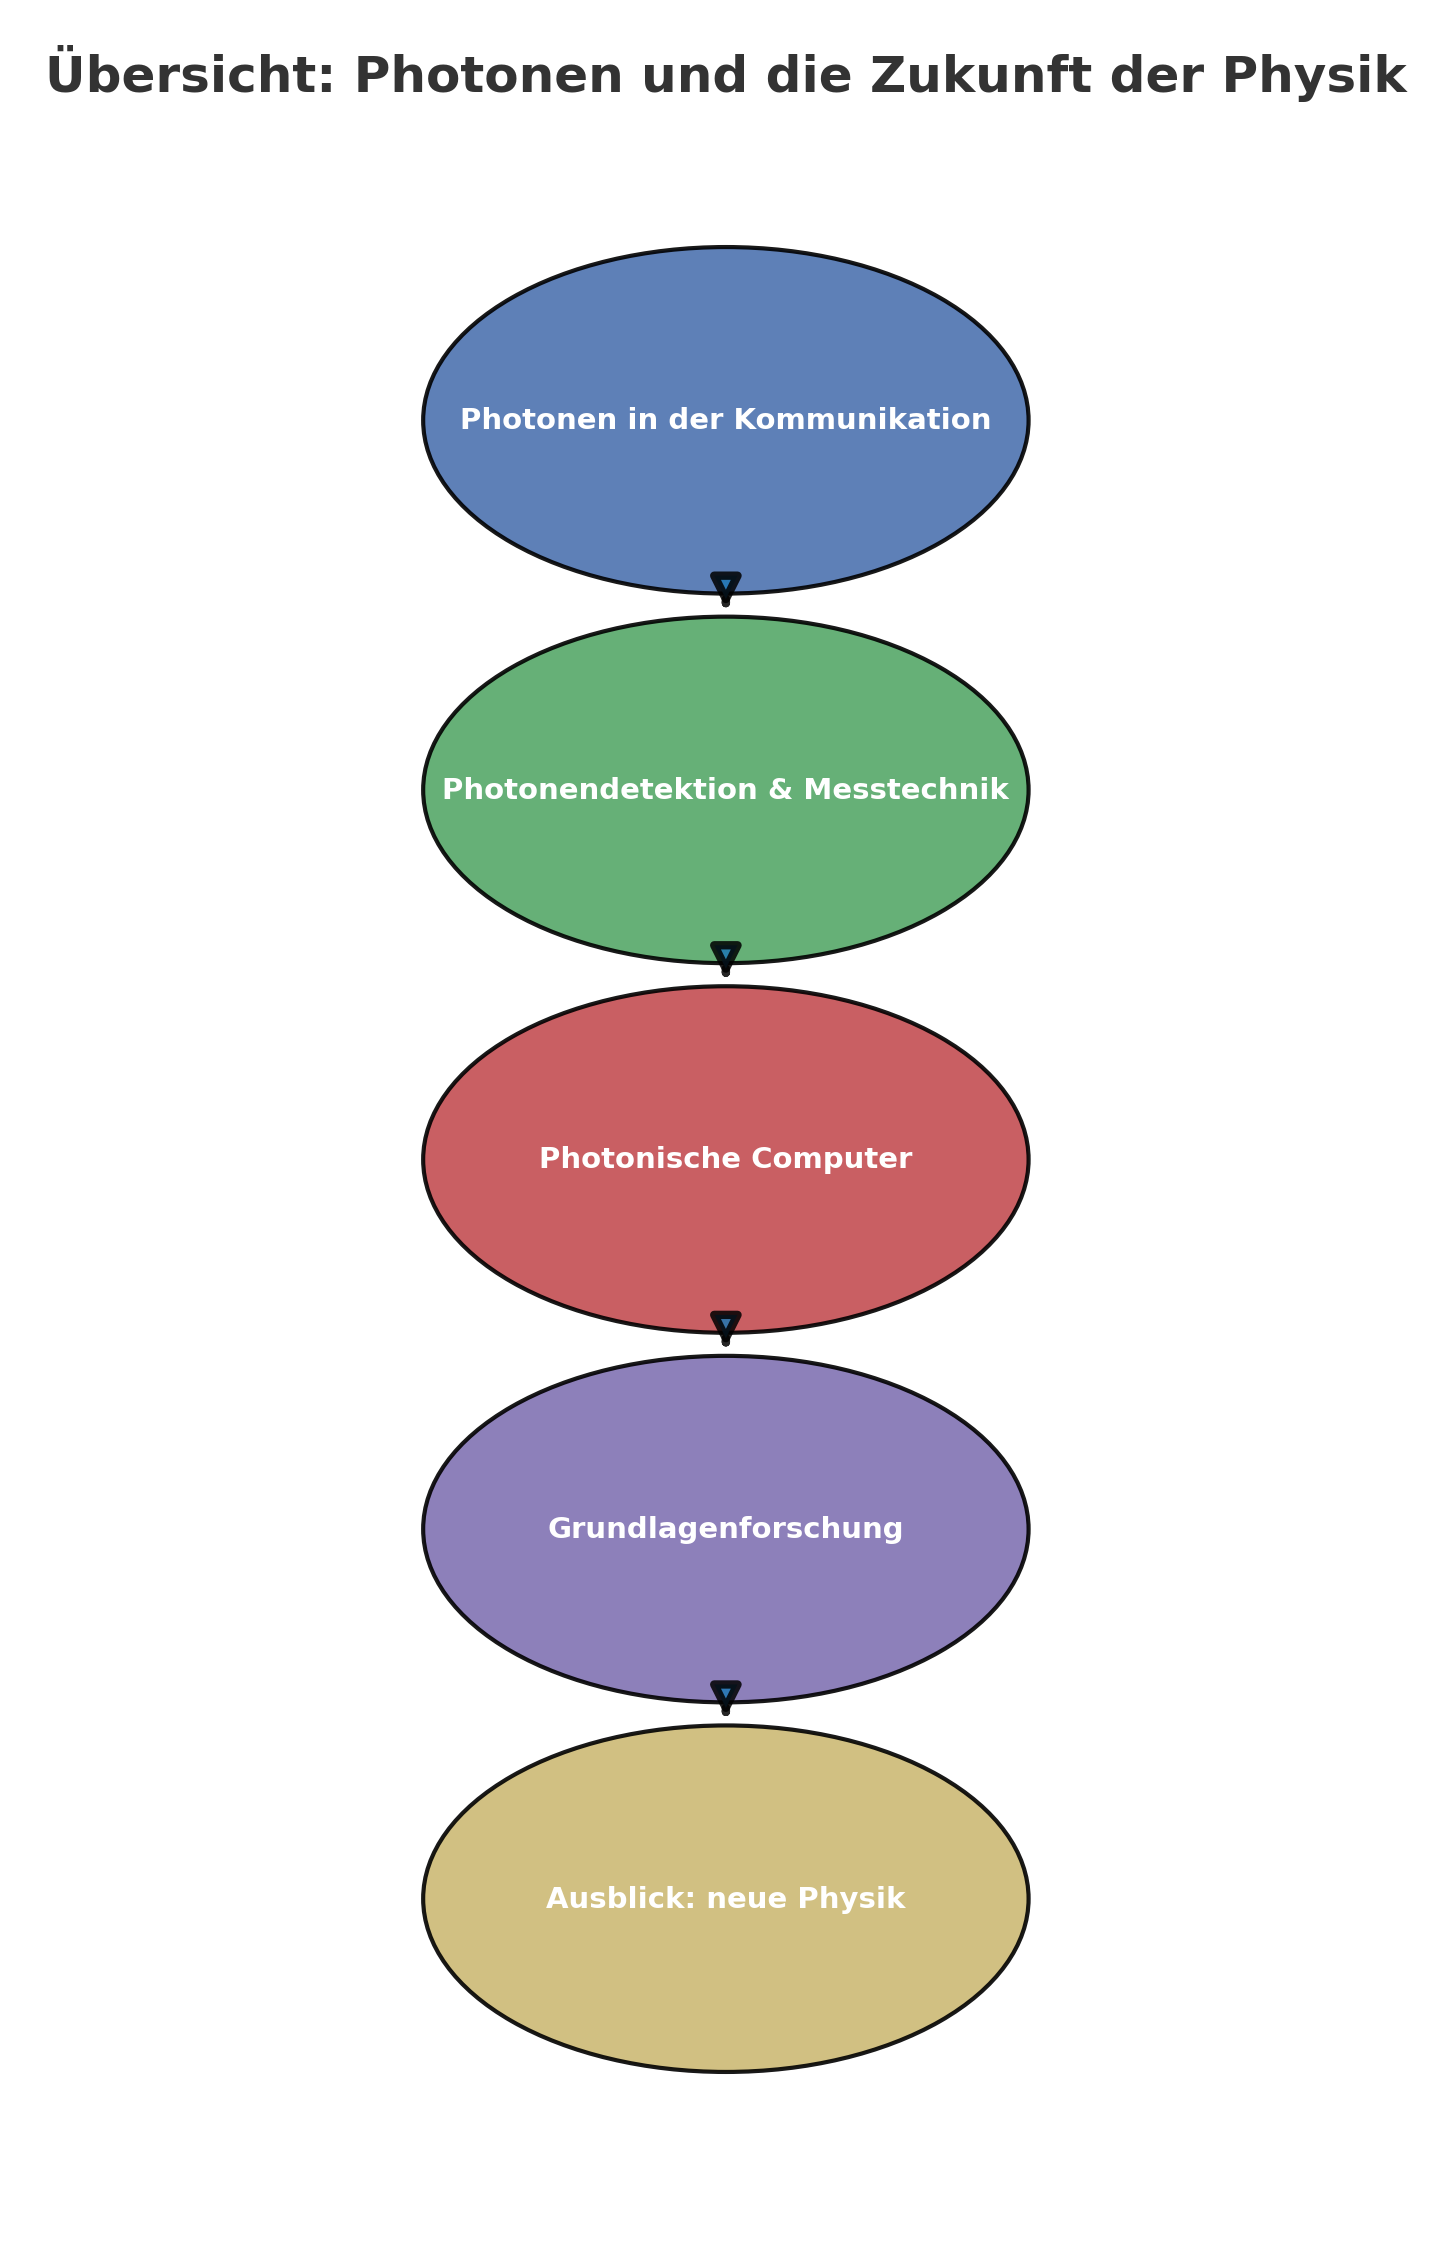
\includegraphics[width=0.75\textwidth]{bilder/kapitel_VII_uebersicht.png}
	\caption[Übersicht Kapitel~VII]{Übersicht: Photonen und die Zukunft der Physik. 
		Die Grafik zeigt die Hauptthemen dieses Kapitels in einer vertikalen Anordnung, 
		von photonischer Logik bis zu offenen Fragen neuer Physik.}
	\label{fig:kapitel_VII_uebersicht}
\end{figure}

\subsection{Einzelphotonen und Quanteninformation}
\index{Einzelphoton}
\index{Quanteninformation}
\index{Qubit}
\index{Superposition}
\index{Polarisation}
\index{Zeit-Bin}
\index{Frequenzkodierung}

Die Fähigkeit, einzelne Photonen gezielt zu erzeugen, zu steuern und zu detektieren, hat in den letzten Jahren eine Schlüsselrolle in der Quanteninformationstechnologie eingenommen. Einzelphotonen dienen als ideale Träger quantenmechanischer Information: Sie sind robust gegenüber Störungen, bewegen sich mit Lichtgeschwindigkeit\index{Lichtgeschwindigkeit} und lassen sich in wohldefinierten Quantenzuständen\index{Quantenzustand} präparieren.

In der klassischen Informationstechnik werden Bits in Form von elektrischen Spannungen oder magnetischen Zuständen gespeichert und verarbeitet. In der Quanteninformation dagegen basiert die kleinste Informationseinheit — das \emph{Qubit} — auf der kohärenten Superposition\index{Superposition} von Zuständen. Bei Photonen werden diese Zustände oft durch Polarisationsrichtungen, Zeit-Bins oder Pfadinformationen realisiert.
\vspace{1em}
\begin{tcolorbox}[physikbox, title=Was macht ein Photon zum Informationsträger? \label{box:photon_information}]
	\small
	Photonen können verschiedene physikalische Freiheitsgrade tragen, die als Qubits nutzbar sind:
	\begin{itemize}
		\item \textbf{Polarisation:} Horizontal ($\ket{H}$) und vertikal ($\ket{V}$) als Basiszustände.
		\item \textbf{Zeit-Bins:} Frühe und späte Ankunftszeiten als logische Zustände.
		\item \textbf{Ort/Pfad:} Zwei verschiedene optische Wege in einem Interferometer\index{Interferometer}.
		\item \textbf{Frequenz:} Unterschiedliche spektrale Modi für kodierte Information.
	\end{itemize}
	Diese Freiheitsgrade lassen sich präzise kontrollieren und über große Distanzen übertragen, ohne dass die Quanteninformation zerstört wird.
\end{tcolorbox}

\subsubsection{Erzeugung von Einzelphotonen}
\index{Einzelphotonenquelle}
\index{Spontane parametrische Fluoreszenz}
\index{Einzelatom}
\index{Ion}
\index{Quantenpunkt}
\index{nichtlinearer Kristall}
\index{Halbleitermaterial}

Einzelphotonenquellen sind zentrale Bausteine der Quantenoptik\index{Quantenoptik}. Gängige Methoden sind:
\begin{itemize}
	\item \emph{Spontane parametrische Fluoreszenz} (SPDC) in nichtlinearen Kristallen.
	\item \emph{Einzelatome} oder Ionen in optischen Fallen\index{optische Falle}.
	\item \emph{Quantenpunkte} in Halbleitermaterialien.
\end{itemize}
Ziel ist es, Photonen mit hoher Reinheit (geringe Mehrphotonenwahrscheinlichkeit) und hoher Indistinguishability (Unterscheidbarkeit) zu erzeugen.
\vspace{1em}
\begin{tcolorbox}[hinweisbox, title=Was bedeutet „Indistinguishability“? \label{box:indistinguishability}]
	\small
	In der Quantenoptik beschreibt \emph{Indistinguishability}, dass zwei Photonen in allen physikalischen Eigenschaften ununterscheidbar sind:
	\begin{itemize}
		\item gleiche Frequenz (Energie)
		\item gleiche Polarisation
		\item identischer räumlicher Modus (gleicher Strahlweg)
		\item identische Ankunftszeit innerhalb der Kohärenzzeit
	\end{itemize}
	Nur wenn Photonen vollkommen indistinguishabel sind, können sie quantenmechanische Interferenzeffekte wie das \emph{Hong–Ou–Mandel-Dip}-Phänomen zeigen.
\end{tcolorbox}
\vspace{1em}
\begin{tcolorbox}[physikbox, title=Das Hong–Ou–Mandel-Dip-Phänomen \label{box:hong_ou_mandel}]
	\small
	Das \emph{Hong–Ou–Mandel-Dip}-Experiment ist ein zentrales Verfahren, um die \emph{Indistinguishability} zweier Photonen zu überprüfen. Treffen zwei ununterscheidbare Photonen gleichzeitig auf einen 50:50-Strahlteiler, verlassen sie diesen stets gemeinsam durch denselben Ausgang — ein reiner Quanteninterferenzeffekt.  
	Die Tiefe des gemessenen „Dips“ in der Koinzidenzrate ist ein direktes Maß für die Ununterscheidbarkeit der Photonen.  
	Eine ausführliche Beschreibung und Abbildung findet sich in \textbf{Kapitel IV.5}.
\end{tcolorbox}

\subsubsection{Dekohärenz und Fehlerquellen}
\index{Dekohärenz}
\index{Quantenfehlerkorrektur}
\index{Quantenrepeater}
\index{Faserdämpfung}
\index{Streuung}
\index{Phasenrauschen}
\index{Vibration}

Quanteninformation ist empfindlich gegenüber Störungen. Bei Photonen sind die Hauptursachen für Dekohärenz:
\begin{itemize}
	\item Wechselwirkung mit dem Übertragungsmedium (z.\,B. Faserdämpfung, Streuung).
	\item Phasenrauschen durch Temperaturschwankungen und Vibrationen.
\end{itemize}
Fehlerkorrektur und Quantenrepeater sind notwendig, um Quanteninformation über weite Strecken zu erhalten.
\newpage
\noindent
\subsubsection{Anwendungen}
\index{Quantenkryptographie}
\index{Satellitenkommunikation}
\index{Hybrid-Quantensystem}

Einzelphotonen bilden die Grundlage für:
\begin{itemize}
	\item Quantenkryptographie.
	\item Quantenkommunikation über Satelliten.
	\item Hybride Systeme, in denen Photonen als Schnittstelle zwischen Materie-Qubits dienen.
\end{itemize}
Diese Anwendungen markieren den Beginn einer neuen Ära der Informationsverarbeitung, in der Photonen nicht nur Träger, sondern auch Vermittler zwischen unterschiedlichen Quantensystemen sind.

\subsection{Quantenkryptographie und Quantenkommunikation} \label{sec:quantum_crypto}
\index{RSA}
\index{Quantencomputer}
\index{Quantenkryptographie}
\index{Quantenkommunikation}
\index{Heisenbergsche Unschärferelation}
\index{No-Cloning-Theorem}
\index{BB84-Protokoll}
\index{Bennett, Charles}
\index{Brassard, Gilles}
\index{Quanten-Schlüsselverteilung}
\index{Satellitenbasierte Quantenkommunikation}
\index{Micius}

Die Sicherheit klassischer Kommunikationssysteme basiert auf mathematischen Verfahren, deren Sicherheit auf der praktischen Unmöglichkeit bestimmter Berechnungen beruht — etwa der Faktorisierung großer Zahlen bei RSA. Diese Sicherheit kann durch zukünftige Quantencomputer gefährdet werden.  
Die Quantenkryptographie hingegen nutzt fundamentale physikalische Gesetze, um die Sicherheit zu gewährleisten — unabhängig von der Rechenleistung eines Angreifers.
\vspace{1em}
\begin{tcolorbox}[physikbox, title=Kernprinzip der Quantenkryptographie \label{box:qcrypto_prinzip}]
	\small
	Die Quantenkryptographie beruht auf zwei zentralen Eigenschaften der Quantenmechanik:
	\begin{enumerate}
		\item \textbf{Messstörung:} Jeder Messversuch an einem Quantenzustand verändert diesen (Heisenbergsche Unschärferelation).
		\item \textbf{Nicht-Klonbarkeit:} Unbekannte Quantenzustände können nicht verlustfrei kopiert werden (No-Cloning-Theorem).
	\end{enumerate}
	Daraus folgt: Abhören hinterlässt unausweichlich Spuren, die von den legitimen Kommunikationspartnern erkannt werden können.
\end{tcolorbox}
\newpage
\noindent
\subsubsection{Quanten-Schlüsselverteilung (QKD)}

Das bekannteste Protokoll ist \textbf{BB84} (Bennett \& Brassard, 1984). Dabei werden einzelne Photonen in zufälligen Polarisationszuständen übertragen.  
Der Ablauf in Kurzform:
\begin{itemize}
	\item Sender (\emph{Alice}) wählt zufällig eine von zwei möglichen Basen (z.\,B. horizontal/vertikal oder diagonal).
	\item Empfänger (\emph{Bob}) misst in zufällig gewählten Basen.
	\item Nach der Übertragung vergleichen beide öffentlich ihre Basiswahl und verwerfen Messungen, bei denen die Basen nicht übereinstimmen.
	\item Aus den verbleibenden Daten wird ein gemeinsamer Schlüssel extrahiert.
\end{itemize}
Ein Abhörversuch (\emph{Eve}) führt zu zusätzlichen Fehlern, die statistisch nachweisbar sind.

\subsubsection{Quantenkommunikation über große Distanzen}

Die Reichweite direkter Quantenkommunikation ist durch Verluste in Glasfasern\index{Glasfaser} und durch atmosphärische Störungen\index{Atmosphäre} begrenzt. Mögliche Lösungen sind:
\begin{itemize}
	\item \textbf{Quantenrepeater:} Knotenpunkte, die verschränkte Photonenpaare\index{verschränkte Photonen} erzeugen und über große Entfernungen verteilen.
	\item \textbf{Satellitenbasierte Quantenkommunikation:} Umgehung der Faserverluste durch freie Übertragung im Weltraum (z.\,B. der chinesische Quantenkommunikationssatellit \emph{Micius}).
\end{itemize}

\subsubsection{Anwendungen und Ausblick}

Quantenkryptographie wird derzeit für hochsichere Regierungs- und Finanzkommunikation getestet. In Kombination mit klassischen Netzwerken entstehen hybride Systeme, die langfristig sichere Kommunikation auch im Zeitalter der Quantencomputer ermöglichen sollen.

Bemerkenswert ist dabei die doppelte Rolle der Quantenphysik:  
Einerseits bedrohen Quantencomputer durch ihre Rechenleistung die Sicherheit heutiger Verschlüsselungsverfahren.  
Andererseits liefert dieselbe Physik mit der Quantenkryptographie einen völlig neuen Ansatz, der prinzipiell abhörsichere Kommunikation erlaubt.  
Dieses Wechselspiel zwischen Herausforderung und Lösung macht die Quantenkommunikation zu einem der spannendsten Forschungsfelder der modernen Physik.

\subsection{Photonik als Zukunftstechnologie}
\index{Laser}
\index{LED}
\index{Glasfaser}
\index{Photonischer Chip}
\index{Photonendetektor}
\index{Modulator}
\index{Filter}
\index{nichtlinearer Kristall}

Photonen sind nicht nur fundamentale Informationsträger in der Quantenphysik, sondern bilden auch die Grundlage zahlreicher moderner Technologien.  
Die \emph{Photonik} umfasst alle Technologien, die auf der Erzeugung, Kontrolle und Detektion von Licht basieren – vom Laser in der Medizin bis zur Glasfaser im weltweiten Kommunikationsnetz.
\vspace{1em}
\begin{tcolorbox}[hinweisbox, title=Was bedeutet „Photonik“? \label{box:photonics_definition}]
	\small
	Der Begriff \emph{Photonik} beschreibt den ingenieurwissenschaftlichen und technologischen Umgang mit Photonen – analog zur Elektronik, die sich mit Elektronen beschäftigt.  
	Photonik umfasst:
	\begin{itemize}
		\item Lichtquellen (Laser, LEDs, Quantenlichtquellen)
		\item Lichtführung (Glasfaser, photonische Chips)
		\item Lichtdetektion (Kameras, Photonendetektoren)
		\item Lichtmanipulation (Modulatoren, Filter, nichtlineare Kristalle)
	\end{itemize}
\end{tcolorbox}

%index
\subsubsection{Photonik in der Kommunikation}
\index{Telekommunikation}
\index{Photonischer Schalter}
\index{Router}
\index{Mikrochip}

In der Telekommunikation ersetzt Photonik zunehmend die Elektronik, um die steigenden Datenmengen zu bewältigen. Glasfasernetze übertragen Informationen mit Lichtgeschwindigkeit und minimalem Energieverlust.  
Photonische Schalter und Router auf Mikrochips versprechen ultraschnelle Signalverarbeitung direkt mit Photonen.

\subsubsection{Photonik in der Medizin}
\index{Laserchirurgie}
\index{optische Kohärenztomographie}
\index{Fluoreszenzdiagnostik}
\index{Biosensor}

Photonische Verfahren wie Laserchirurgie, optische Bildgebung (OCT) und fluoreszenzbasierte Diagnostik haben die Medizin revolutioniert.  
Zukünftige Entwicklungen umfassen minimalinvasive Operationen mit ultrakurzen Laserpulsen und photonische Biosensoren für Echtzeitdiagnosen.

\subsubsection{Photonik in der Sensorik und Messtechnik}
\index{Photonischer Sensor}
\index{LIDAR}
\index{Gravitationswellendetektor}

Photonische Sensoren ermöglichen hochpräzise Messungen in Industrie, Geowissenschaften und Raumfahrt.  
Beispiele sind LIDAR-Systeme für autonomes Fahren und interferometrische Gravitationswellendetektoren.

\vspace{1em}
\begin{tcolorbox}[physikbox, title=Photonische Schaltungen vs. Elektronische Schaltungen \label{box:photon_vs_electron}]
	\small
	Photonische Schaltungen bieten gegenüber elektronischen Ansätzen mehrere entscheidende Vorteile:
	\begin{itemize}
		\item \textbf{Höhere Geschwindigkeit:} Licht bewegt sich im Medium deutlich schneller als Elektronen in Leitern.
		\item \textbf{Geringere Verluste:} Keine ohmsche Erwärmung durch elektrischen Widerstand.
		\item \textbf{Höhere Bandbreite:} Ein Photonensignal kann viele Wellenlängen (Multiplexing) gleichzeitig tragen.
		\item \textbf{Geringe Übersprechung:} Kaum elektromagnetische Störeinflüsse zwischen benachbarten Leitungen.
	\end{itemize}
	Diese Eigenschaften machen photonische Schaltungen zu einem Schlüsselfaktor für zukünftige Hochgeschwindigkeits- und Hochbandbreitentechnologien.
\end{tcolorbox}

\subsubsection{Ausblick}

Photonik gilt als Schlüsseltechnologie des 21. Jahrhunderts. Ihre Kombination mit der Quantenphysik – etwa in Quantenkommunikation, Quantencomputern oder Quantenmetrologie – verspricht völlig neue Anwendungen.  
Die Entwicklung hin zu integrierten photonischen Schaltkreisen könnte in der Informationsverarbeitung einen ähnlichen Umbruch auslösen wie die Mikroelektronik im 20. Jahrhundert.

\subsection{Optische Logik und photonische Computer}
\index{Optische Logik}
\index{Mach--Zehnder-Interferometer}
\index{Mikroresonator}
\index{Optischer Modulator}

Die Miniaturisierung elektronischer Schaltkreise stößt zunehmend an physikalische Grenzen: Transistoren werden so klein, dass Quanten- und Wärmeeffekte ihre Funktion beeinträchtigen. Gleichzeitig steigt der Energiebedarf moderner Rechenzentren rasant. Eine vielversprechende Alternative ist die Nutzung von Photonen anstelle von Elektronen zur Informationsverarbeitung.
\vspace{1em}
\begin{tcolorbox}[physikbox, title=Warum Photonen für Logikschaltungen interessant sind, label=box:optlogik_vorteile]
	\small
	\begin{itemize}
		\item \textbf{Hohe Geschwindigkeit:} Licht bewegt sich nahezu mit Lichtgeschwindigkeit – optische Signale können extrem schnell verarbeitet werden.
		\item \textbf{Keine ohmschen Verluste:} Im Gegensatz zu elektrischen Strömen erwärmen sich optische Leitungen kaum.
		\item \textbf{Parallele Verarbeitung:} Durch Multiplexing können mehrere Wellenlängen gleichzeitig genutzt werden.
		\item \textbf{Direkte Kopplung an Glasfaser-Kommunikation:} Keine Umwandlung zwischen Elektronen- und Photonen-Signalen nötig.
	\end{itemize}
\end{tcolorbox}

\subsubsection{Grundprinzip optischer Logikgatter}
\index{Optisches Logikgatter}
\index{Photonischer Kristall}

Optische Logikschaltungen arbeiten mit Bauelementen, die Lichtstrahlen abhängig von Eingangsbedingungen umleiten, abschwächen oder verstärken. Beispiele sind nichtlineare Kristalle, optische Modulatoren oder photonische Kristallstrukturen.  
Logikgatter wie \textsc{AND}, \textsc{OR} und \textsc{NOT} lassen sich dabei durch Interferenz, Absorption oder Polarisationsänderung realisieren.
\vspace{1em}
\begin{tcolorbox}[didaktikbox, title=Von Elektronik zu Photonik]
	\label{box:optlogik_didaktik}
	\small
	In der Elektronik basieren Logikgatter auf Transistoren, die den Stromfluss blockieren oder freigeben. In der Photonik übernehmen Bauelemente wie Mach–Zehnder-Interferometer oder Mikroresonatoren diese Aufgabe – nur eben für Licht.
\end{tcolorbox}

\subsubsection{Photonische Computer}
\index{Photonischer Computer}
\index{Künstliche Intelligenz}
\index{Signalverarbeitung}
\index{Quanteninformationsverarbeitung}

Ein photonischer Computer nutzt optische Schaltungen für zentrale Rechenoperationen. Besonders geeignet ist diese Technik für:
\begin{itemize}
	\item \textbf{Künstliche Intelligenz:} Matrixmultiplikationen können extrem schnell und energieeffizient in optischen Netzwerken durchgeführt werden.
	\item \textbf{Signalverarbeitung:} Breitbandige Verarbeitung ohne elektrische Engpässe.
	\item \textbf{Quanteninformationsverarbeitung:} Kombination aus photonischer Logik und Quantenbits (Qubits).
\end{itemize}
\vspace{1em}
\begin{tcolorbox}[hypobox, title={Was wäre, wenn optische Computer Elektronik ablösen?}]
	\label{box:optlogik_zukunft}
	\small
	Falls photonische Computer die Elektronik vollständig ersetzen könnten, ließe sich der Energieverbrauch großer Rechenzentren drastisch senken. Gleichzeitig könnten Taktraten im Terahertz-Bereich erreicht werden – weit jenseits heutiger Prozessoren.
\end{tcolorbox}
Optische Logikgatter lassen sich auch mit einem Mach–Zehnder-Interferometer (MZI) realisieren. 
Dabei teilt ein Strahlteiler den Laserstrahl in zwei Pfade, in denen jeweils ein Phasenmodulator sitzt. 
Nur wenn beide Modulatoren eine bestimmte Phasenverschiebung setzen, interferieren die beiden Strahlen am zweiten Strahlteiler so, dass Licht am gewünschten Ausgang erscheint. 
Wählt man die Phasen so, dass dies nur bei zwei aktiven Eingaben geschieht, arbeitet das MZI wie ein klassisches \textsc{AND}-Gatter – allerdings auf rein optischem Weg. 
%Eine kompakte Wahrheitstabelle und die genaue Funktionsweise sind in \ref{sec:mzi_and_detail} beschrieben.
\vspace{1em}
\begin{tcolorbox}[didaktikbox, title=Photonisches AND-Gatter im Mach--Zehnder-Interferometer, label={box:mzi_and}]
	\small
	Ein Mach--Zehnder-Interferometer kann so beschaltet werden, dass es wie ein \textsc{AND}-Gatter arbeitet. 
	Die Eingänge \(A\) und \(B\) steuern Phasenmodulatoren in den beiden Armen des Interferometers. 
	Nur wenn beide eine Phasenverschiebung von \(\pi\) setzen, addieren sich die Phasen zu \(2\pi\) und es kommt zu konstruktiver Interferenz am „1“-Ausgang.
	
	\begin{center}
		\begin{tabular}{c c c c c c}
			\toprule
			\(A\) & \(B\) & Phase A & Phase B & Ausgang „1“ & Ausgang „0“ \\
			\midrule
			0 & 0 & \(0\) & \(0\) & 1 & 0 \\
			0 & 1 & \(0\) & \(\pi\) & 0 & 1 \\
			1 & 0 & \(\pi\) & \(0\) & 0 & 1 \\
			1 & 1 & \(\pi\) & \(\pi\) & 1 & 0 \\
			\bottomrule
		\end{tabular}
	\end{center}
	
	Nur bei \(A=1\) und \(B=1\) ist die Gesamtphase \(2\pi\), sodass der obere Ausgang hell wird. 
	In allen anderen Fällen wird das Licht in den „0“-Ausgang gelenkt.
\end{tcolorbox}
\begin{figure}[H]
	\centering
	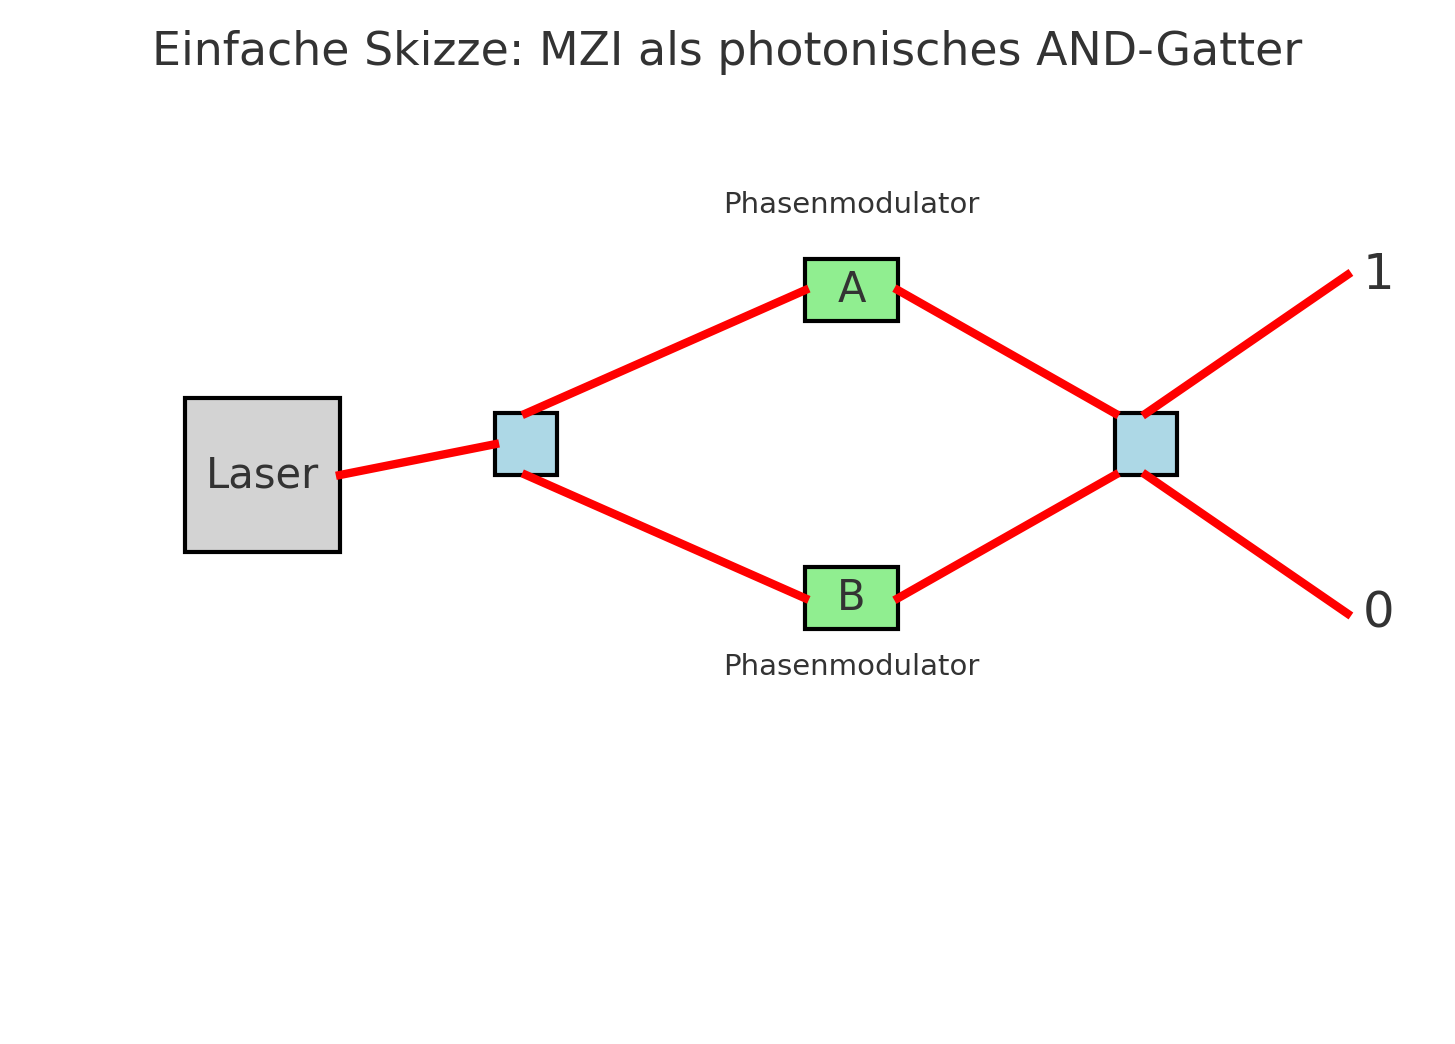
\includegraphics[width=0.75\textwidth]{bilder/mzi_and_simple.png} % <-- Pfad anpassen
	\caption{Einfache schematische Darstellung eines Mach--Zehnder-Interferometers mit zwei Phasenmodulatoren (\(A\) und \(B\)), das als photonisches \textsc{AND}-Gatter arbeitet. Nur wenn beide Modulatoren eine Phasenverschiebung von \(\pi\) setzen, addieren sich die Phasen zu \(2\pi\) und es erscheint Licht am „1“-Ausgang.}
	\label{fig:mzi_and_simple}
\end{figure}

\subsubsection{Herausforderungen}
\index{Chip-Integration}
\index{Miniaturisierung}
\index{Elektronik-Integration}

Trotz der Vorteile gibt es noch offene Probleme:
\begin{itemize}
	\item Effiziente Erzeugung und Kontrolle einzelner Photonen auf Chip-Ebene.
	\item Miniaturisierung optischer Bauteile auf Nanometermaßstab.
	\item Integration mit bestehender Elektronik.
\end{itemize}

\subsubsection{Zusammenfassung}

Optische Logik und photonische Computer bieten eine faszinierende Möglichkeit, die Rechenleistung zu steigern und den Energiebedarf zu senken. Ob sie die klassische Elektronik komplett ablösen oder nur in Spezialanwendungen dominieren werden, hängt von der Lösung der technischen Herausforderungen ab.
\newpage
\noindent
\subsection{Photonen in der Grundlagenforschung}
\index{Boson}
\index{Kosmologie}
\index{Kosmischer Mikrowellenhintergrund}
\index{Bell-Test}
\index{Quantentomographie}
\index{Gravitationslinse}
\index{Lorentz-Invarianz}
\index{CPT-Symmetrie}

Photonen spielen nicht nur in der Technik, sondern auch in der modernen Grundlagenforschung eine zentrale Rolle. 
Ihre Eigenschaften als masselose, bosonische Quantenobjekte machen sie zu idealen Werkzeugen, um fundamentale Fragen der Physik zu untersuchen – vom kleinsten Maßstab der Quantenmechanik bis zu kosmologischen Distanzen.

\begin{itemize}
	\item \textbf{Prüfung der Quantenmechanik:} Experimente mit einzelnen Photonen – etwa Doppelspaltversuche, Bell-Tests oder Quantentomographie – testen die Grenzen und Vorhersagen der Quantenmechanik mit höchster Präzision.
	\item \textbf{Astrophysik und Kosmologie:} Photonen aus fernen Galaxien und dem kosmischen Mikrowellenhintergrund liefern Informationen über die Entstehung und Entwicklung des Universums.
	\item \textbf{Präzisionsmessungen:} Laserinterferometer wie LIGO oder Virgo detektieren winzige Längenänderungen durch Gravitationswellen – basierend auf kohärenten Photonenstrahlen.
	\item \textbf{Tests fundamentaler Symmetrien:} Polarisation, Frequenz und Flugzeit von Photonen werden genutzt, um Lorentz-Invarianz, CPT-Symmetrie und andere fundamentale Prinzipien zu überprüfen.
	
\end{itemize}
\vspace{1em}
\begin{tcolorbox}[physikbox, title={Photonen als Boten der Naturgesetze}, label={box:photonen_grundlagen}]
	\small
	Photonen interagieren nur schwach mit ihrer Umgebung, bewegen sich mit Lichtgeschwindigkeit und tragen Informationen über ihre Quelle über Milliarden Jahre und Lichtjahre hinweg. 
	Dies macht sie zu einzigartigen Boten, die uns Einblicke in Prozesse geben, die weder direkt zugänglich noch reproduzierbar sind – von den ersten Momenten nach dem Urknall bis hin zu den subtilsten Effekten in der Quantenfeldtheorie.
\end{tcolorbox}
\begin{figure}[H]
	\centering
	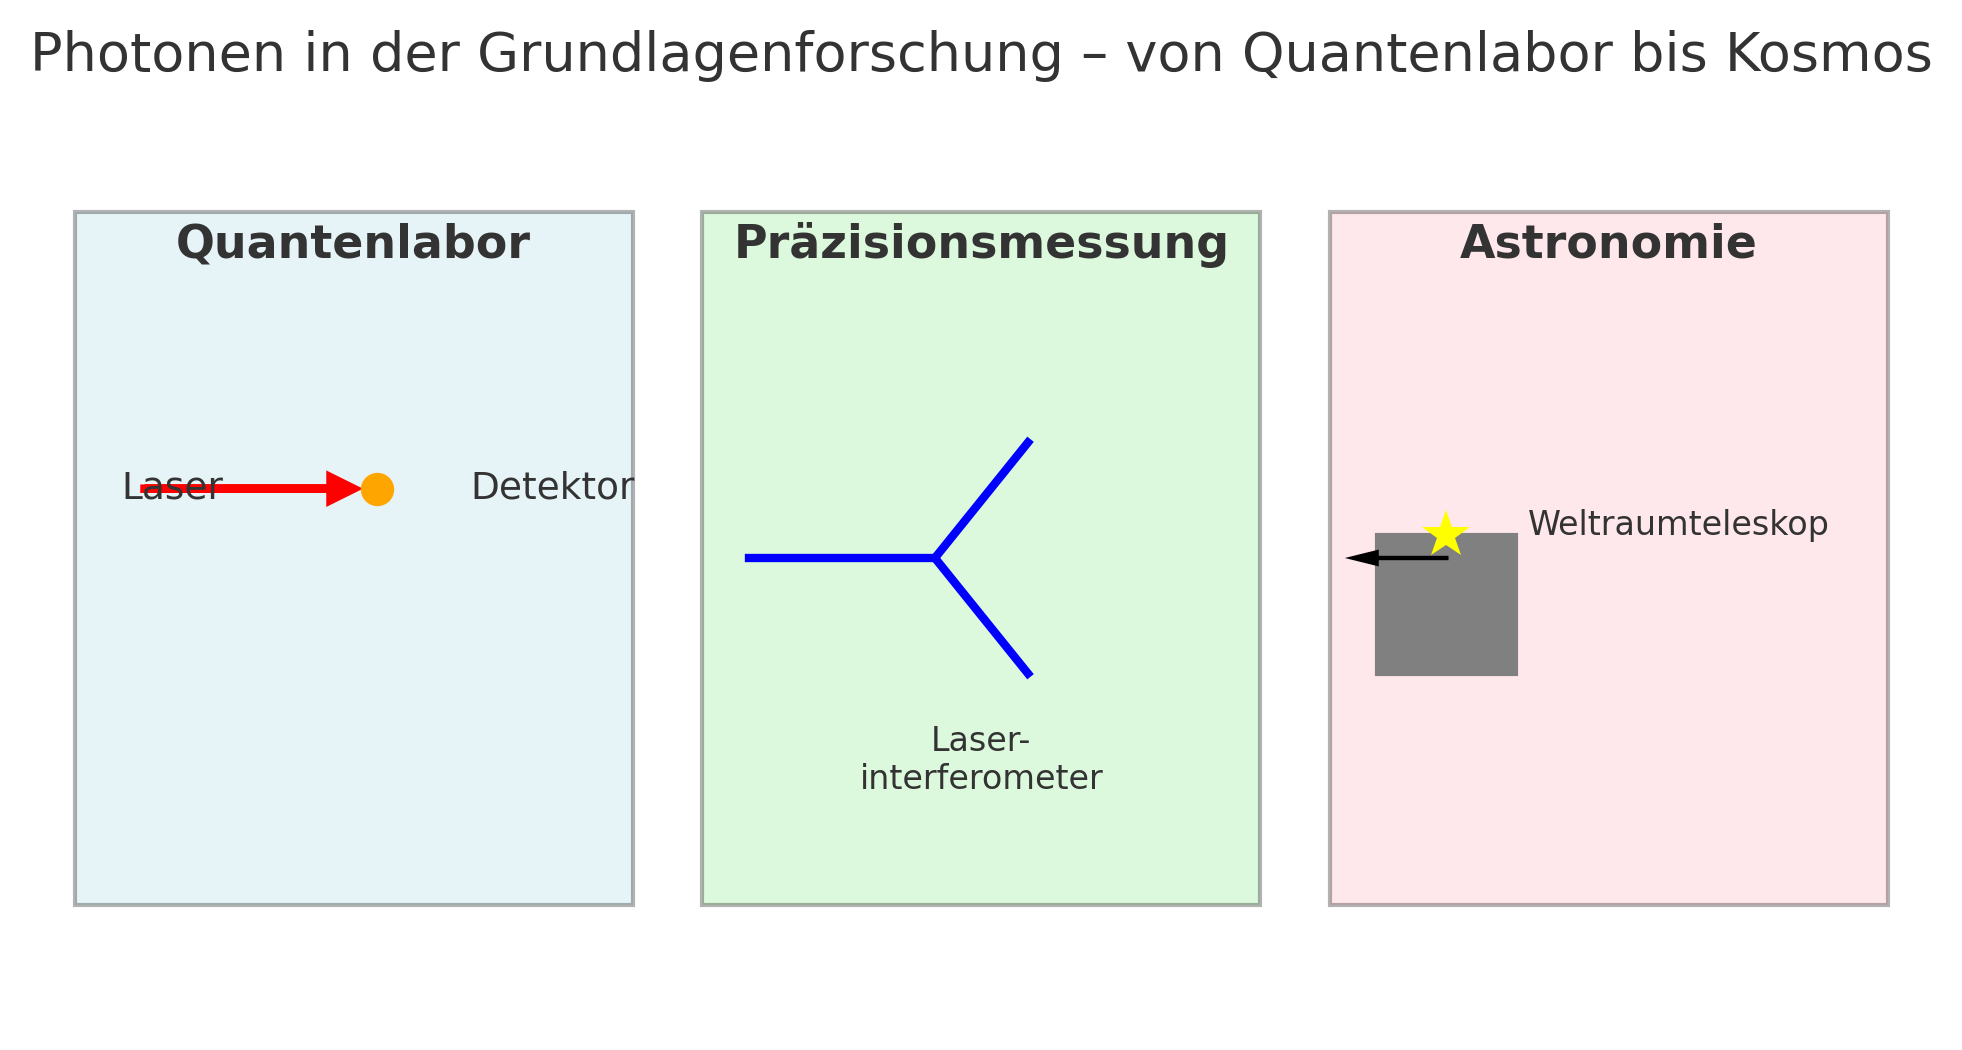
\includegraphics[width=0.9\textwidth]{bilder/photonen_grundlagenforschung.png} % <-- Pfad anpassen
	\caption{Photonen in der Grundlagenforschung: 
		vom Quantenlabor über Präzisionsmessungen bis hin zur Astronomie. 
		Die Illustration zeigt Beispiele für zentrale Einsatzbereiche: 
		Experimente mit einzelnen Photonen im Labor, Laserinterferometrie für Gravitationswellendetektion und weltraumgestützte Beobachtungen von Sternen und Galaxien.}
	\label{fig:photonen_grundlagen}
\end{figure}

\subsubsection{Ausblick}

Die Grundlagenforschung mit Photonen ist längst nicht abgeschlossen. 
Neue Detektionsmethoden, verbesserte Quellen für einzelne und verschränkte Photonen sowie weltraumgestützte Experimente versprechen noch tiefere Einblicke in die Struktur der Naturgesetze.
\newpage
\noindent
\subsection{Ausblick: Graviton, Dunkle Energie, neue \newline Physik?}
\index{Neue Physik}

Auch wenn das Photon als Lichtquant in der modernen Physik bestens verstanden ist, bleiben viele fundamentale Fragen offen – und Photonen spielen bei deren Beantwortung oft eine Schlüsselrolle.

\begin{itemize}
	\item \textbf{Das Graviton:} Das hypothetische Austauschteilchen der Gravitation wurde bisher nicht nachgewiesen. 
	Präzise Messungen mit Photonen – etwa über Gravitationslinsen oder Interferometrie – könnten indirekte Hinweise liefern.
	\item \textbf{Dunkle Energie:} Die beschleunigte Expansion des Universums deutet auf eine bislang unbekannte Form von Energie hin. 
	Photometrie und Spektroskopie entfernter Supernovae und Galaxien nutzen Photonen als einzige Informationsquelle, um diese rätselhafte Komponente zu untersuchen.
	\item \textbf{Neue Physik jenseits des Standardmodells:} Hochpräzise Experimente mit Photonen könnten Abweichungen von etablierten Theorien aufdecken, etwa winzige Verletzungen der Lorentz-Invarianz oder Hinweise auf zusätzliche Raumdimensionen.
\end{itemize}

\begin{tcolorbox}[hypobox, title={Was wäre, wenn das Photon nicht das einzige masselose Boson wäre?}, label={box:photon_neue_physik}]
	\small
	Die Existenz weiterer masseloser Austauschteilchen – etwa des Gravitons – würde unser Verständnis der fundamentalen Kräfte grundlegend verändern. 
	Photonenexperimente könnten über subtile Effekte, wie Abweichungen in der Lichtausbreitung oder Polarisationsmuster, erste Hinweise auf eine solche neue Physik liefern.
\end{tcolorbox}
\begin{figure}[H]
	\centering
	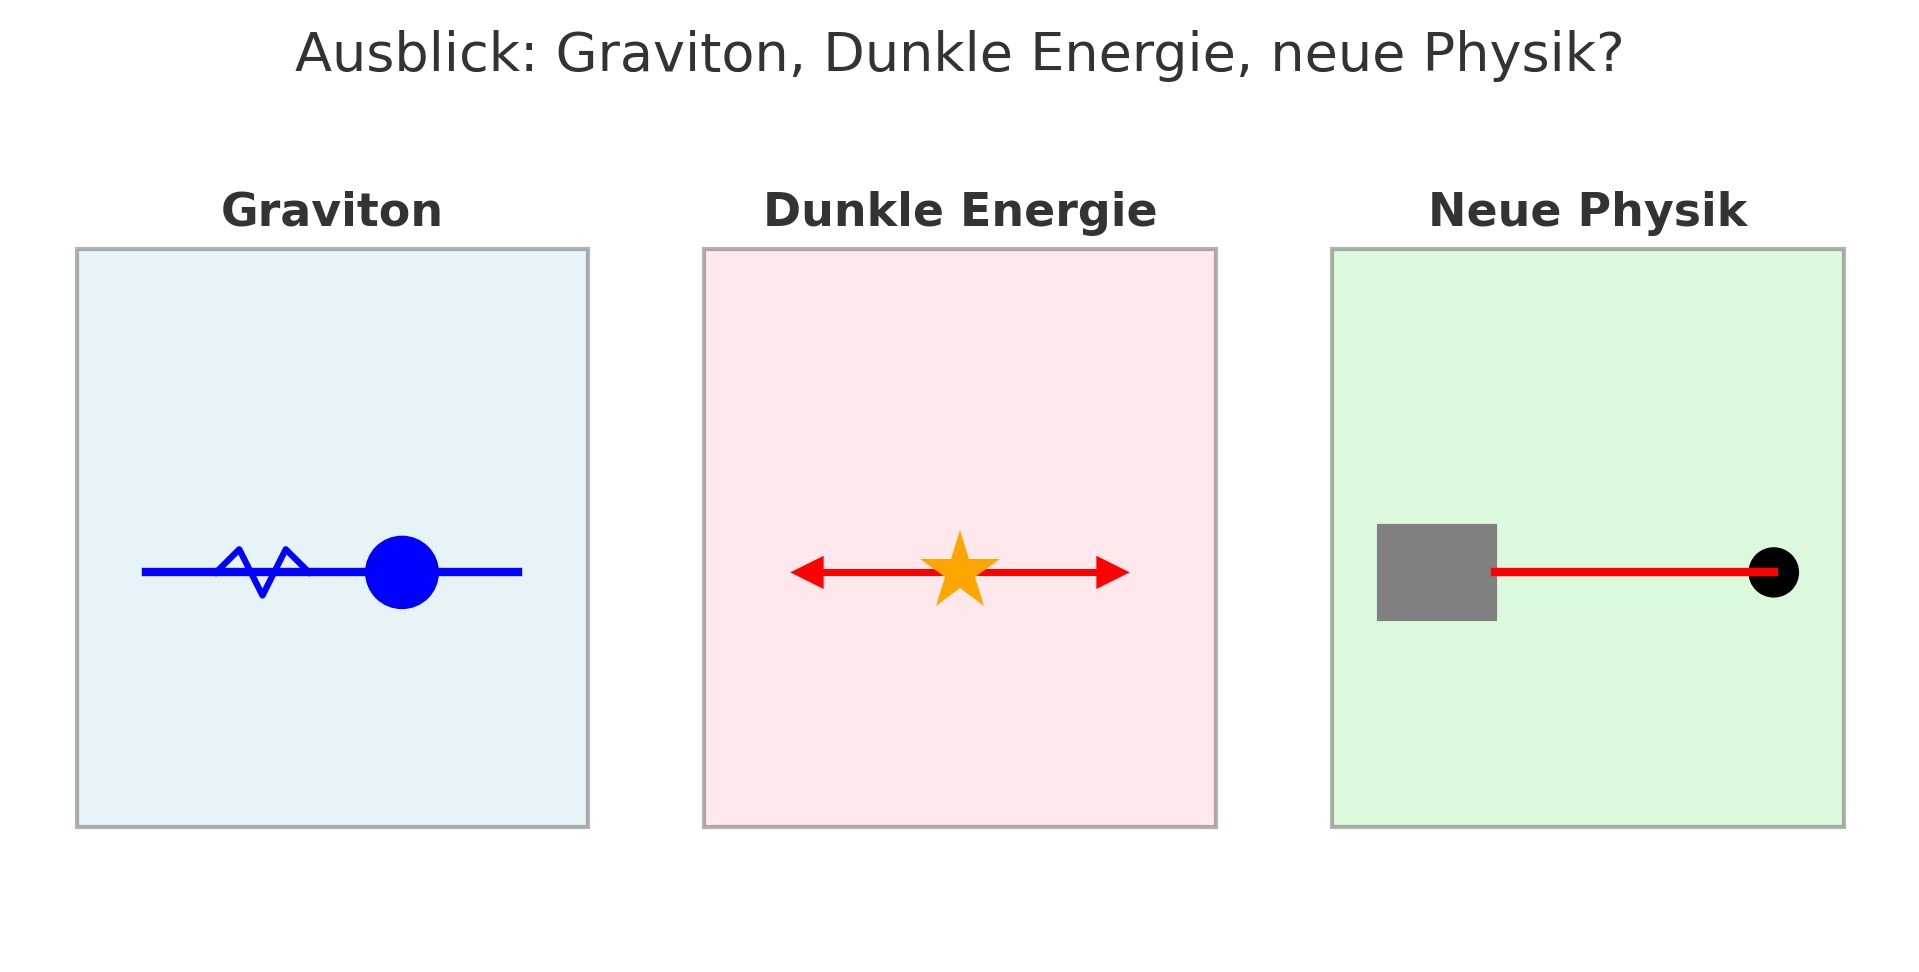
\includegraphics[width=0.9\textwidth]{bilder/photonen_ausblick_fixed.png} % <-- Pfad anpassen
	\caption{Symbolische Darstellung des Ausblicks auf offene Fragen in der Physik:
		\textbf{links:} das hypothetische Graviton als möglicher weiterer masseloser Austauschteilchen-Kandidat;
		\textbf{Mitte:} Dunkle Energie, erkennbar durch die beschleunigte Expansion des Universums;
		\textbf{rechts:} Labor-Experimente mit Photonen, die nach Hinweisen auf neue Physik suchen.}
	\label{fig:photonen_ausblick}
\end{figure}

\subsubsection{Ausblick}

Die Zukunft der Photonenforschung liegt nicht nur in technischen Anwendungen, sondern auch in der Rolle des Photons als präzisem Boten neuer Naturgesetze. 
Weltraumteleskope, Gravitationswellenobservatorien und Labor-Experimente mit nie dagewesener Empfindlichkeit könnten uns der Beantwortung dieser fundamentalen Fragen näherbringen.

\subsection{Fazit}

Photonen sind weit mehr als nur Träger von Licht – sie sind Werkzeuge, Datenüberträger, Messinstrumente und Boten der fundamentalen Gesetze der Natur. 
Von optischer Kommunikation und präziser Messtechnik über photonische Computer bis hin zur Untersuchung kosmischer Phänomene zeigt sich ihre Vielseitigkeit. 
Die hier vorgestellten Anwendungen verdeutlichen, dass Photonen nicht nur die Grundlage moderner Technologien bilden, sondern auch entscheidend für die Erforschung offener Fragen der Physik sind – von der Natur der Gravitation über die Dunkle Energie bis hin zu möglichen Erweiterungen des Standardmodells. 
Die Zukunft der Photonenforschung liegt daher gleichermaßen in der Weiterentwicklung technischer Systeme wie in der Suche nach neuer Physik.

\medskip
\emph{Das Photon ist nicht nur ein Lichtteilchen – es ist ein Schlüssel zur Technologie von heute und zur Physik von morgen.}
\vspace{1em}
\begin{tcolorbox}[hypobox, title={Was wäre, wenn wir Photonen völlig kontrollieren könnten?}]
	\label{box:hypo_kapVII}
	Ein Gedankenexperiment: 
	\begin{itemize}
		\item Photonenchips könnten klassische Elektronik ablösen – mit nahezu lichtschnellen Berechnungen.
		\item Globale Quantenkommunikationsnetze wären absolut abhörsicher.
		\item Einzelphotonen-Labore könnten medizinische Diagnosen auf molekularer Ebene revolutionieren.
		\item Photonen als „Sonden“ könnten uns direkte Einblicke in Dunkle Materie oder die Struktur der Raumzeit geben.
	\end{itemize}
	\medskip
	Solche visionären Szenarien gehen über heutige Technik hinaus – sie bilden die Brücke zum nächsten Kapitel über \emph{Photonen im Standardmodell und visionäre Anwendungen}.
\end{tcolorbox}

	\chapter{Das Photon im Standardmodell der Teilchenphysik}
\setcounter{section}{8}
\setcounter{subsection}{0}
\setcounter{subsubsection}{1}
\setcounter{secnumdepth}{3}
% Boxen-Stile definieren
\tcbset{physikbox/.style={colback=blue!5!white, colframe=blue!75!black, fonttitle=\bfseries}}
\tcbset{mathebox/.style={colback=green!5!white, colframe=green!50!black, fonttitle=\bfseries}}
\tcbset{didaktikbox/.style={colback=yellow!5!white, colframe=yellow!50!black, fonttitle=\bfseries}}
\tcbset{hypobox/.style={colback=orange!5!white, colframe=orange!75!black, fonttitle=\bfseries}}
\tcbset{hinweisbox/.style={colback=gray!10!white, colframe=black!40!black, fonttitle=\bfseries}}

\subsection{Das Standardmodell: Überblick}

Das \textbf{Standardmodell der Teilchenphysik}\index{Standardmodell der Teilchenphysik} ist eine erfolgreiche Theorie, die die bekannten fundamentalen Teilchen und ihre Wechselwirkungen – mit Ausnahme der \textbf{Gravitation}\index{Gravitation} – beschreibt.  
Es kombiniert die \textbf{Quantenelektrodynamik (QED)}\index{Quantenelektrodynamik (QED)}, die \textbf{Quantentheorie der schwachen Wechselwirkung}\index{Schwache Wechselwirkung} und die \textbf{Quantenchromodynamik (QCD)}\index{Quantenchromodynamik (QCD)} zu einem konsistenten Rahmenwerk.

Die fundamentalen Bausteine sind \textbf{Fermionen}\index{Fermion}, die Materie bilden, und \textbf{Bosonen}\index{Boson}, die als Austauschteilchen für die fundamentalen Kräfte wirken.  
Bosonen sind Teilchen mit ganzzahligem Spin, die durch ihre Austauschwirkung die fundamentalen Kräfte vermitteln.  
Zu den Eichbosonen\index{Eichboson} zählen das \textbf{Photon}\index{Photon} (Träger der elektromagnetischen Wechselwirkung), die \textbf{$W^\pm$- und $Z^0$-Bosonen}\index{W-Boson}\index{Z-Boson} (Träger der schwachen Wechselwirkung) sowie die \textbf{Gluonen}\index{Gluon} (Träger der starken Wechselwirkung).  
Das \textbf{Higgs-Boson}\index{Higgs-Boson} spielt eine besondere Rolle: Es verleiht den Elementarteilchen über den \textbf{Higgs-Mechanismus}\index{Higgs-Mechanismus} ihre Masse.

Die Wechselwirkungen werden durch \textbf{Eichsymmetrien}\index{Eichsymmetrie} beschrieben, die in der mathematischen Sprache von \textbf{Lie-Gruppen}\index{Lie-Gruppe} formuliert sind.  
Das Standardmodell basiert auf der Symmetriegruppe \(\mathrm{SU(3)} \times \mathrm{SU(2)} \times \mathrm{U(1)}\)\index{SU(3)}\index{SU(2)}\index{U(1)}.  
Jeder dieser Faktoren steht für eine fundamentale Wechselwirkung:  
\(\mathrm{SU(3)}\) für die starke Wechselwirkung, \(\mathrm{SU(2)} \times \mathrm{U(1)}\) für die \textbf{elektroschwache Theorie}\index{Elektroschwache Theorie}.

Trotz seines Erfolges ist das Standardmodell unvollständig:  
Es erklärt weder die Gravitation, noch liefert es Antworten auf Fragen nach \textbf{Dunkler Materie}\index{Dunkle Materie} oder \textbf{Dunkler Energie}\index{Dunkle Energie}.

\subsection{U(1)-Eichsymmetrie und das Photon}



Die elektromagnetische Wechselwirkung lässt sich elegant als \textbf{U(1)-Eich\-symmetrie}\index{U(1)-Eichsymmetrie} formulieren.  
Die Gruppe \(\mathrm{U(1)}\)\index{U(1)} ist die Menge aller komplexen Zahlen mit Betrag 1, die sich in der Form \(e^{i\theta}\) darstellen lassen.  
Sie ist eine \textbf{abelsche Gruppe}\index{Abelsche Gruppe}, d.\,h. die Gruppenoperation (hier: Multiplikation) ist kommutativ.  
In der Sprache der Mathematik gehört \(\mathrm{U(1)}\) zu den \textbf{Lie-Gruppen}\index{Lie-Gruppe}, also zu stetigen Symmetriegruppen, deren Elemente durch stetige Parameter beschrieben werden.

In der Quantenmechanik beschreibt eine \textbf{globale U(1)-Symmetrie}\index{Globale Symmetrie} die Invarianz der Wellenfunktion unter einer Phasenänderung \(\psi \to e^{i\alpha}\psi\).  
Nach dem \textbf{Noether-Theorem}\index{Noether-Theorem} ist diese Symmetrie direkt mit der \textbf{Ladungserhaltung}\index{Ladungserhaltung} verknüpft.

Wird die Symmetrie \emph{lokal} gemacht – d.\,h. der Phasenwinkel \(\alpha\) darf von Raum und Zeit abhängen –, spricht man von einer \textbf{lokalen U(1)-Eichsymmetrie}\index{Lokale Symmetrie}.  
Damit diese Invarianz erhalten bleibt, muss ein neues Feld eingeführt werden: das elektromagnetische Potential \(A_\mu\)\index{Elektromagnetisches Potential}.  
Dieses Feld kompensiert die Änderungen der Phase und führt zur \textbf{Eichkopplung}\index{Eichkopplung} zwischen geladenen Teilchen und dem Feld.

Die Quantisierung dieses Feldes liefert das \textbf{Photon}\index{Photon} als masseloses \textbf{Eichboson}\index{Eichboson} der elektromagnetischen Wechselwirkung.  
Seine Eigenschaften – insbesondere Masselosigkeit und Spin 1 – folgen direkt aus der Struktur der U(1)-Symmetrie.

Die U(1)-Eichtheorie ist ein Spezialfall einer abelschen Eichtheorie\index{Abelsche Eichtheorie} und bildet den elektromagnetischen Sektor der \textbf{elektroschwachen Theorie}\index{Elektroschwache Theorie}.  
Ihre mathematische Einfachheit macht sie zu einem idealen Ausgangspunkt, um komplexere Theorien wie \(\mathrm{SU(2)}\) oder \(\mathrm{SU(3)}\) zu verstehen.
\vspace{1em}
\begin{tcolorbox}[didaktikbox, title=U(1) anschaulich erklärt]
	\label{box:u1_kreis}
	\small
	\begin{minipage}{0.35\textwidth}
		\centering
		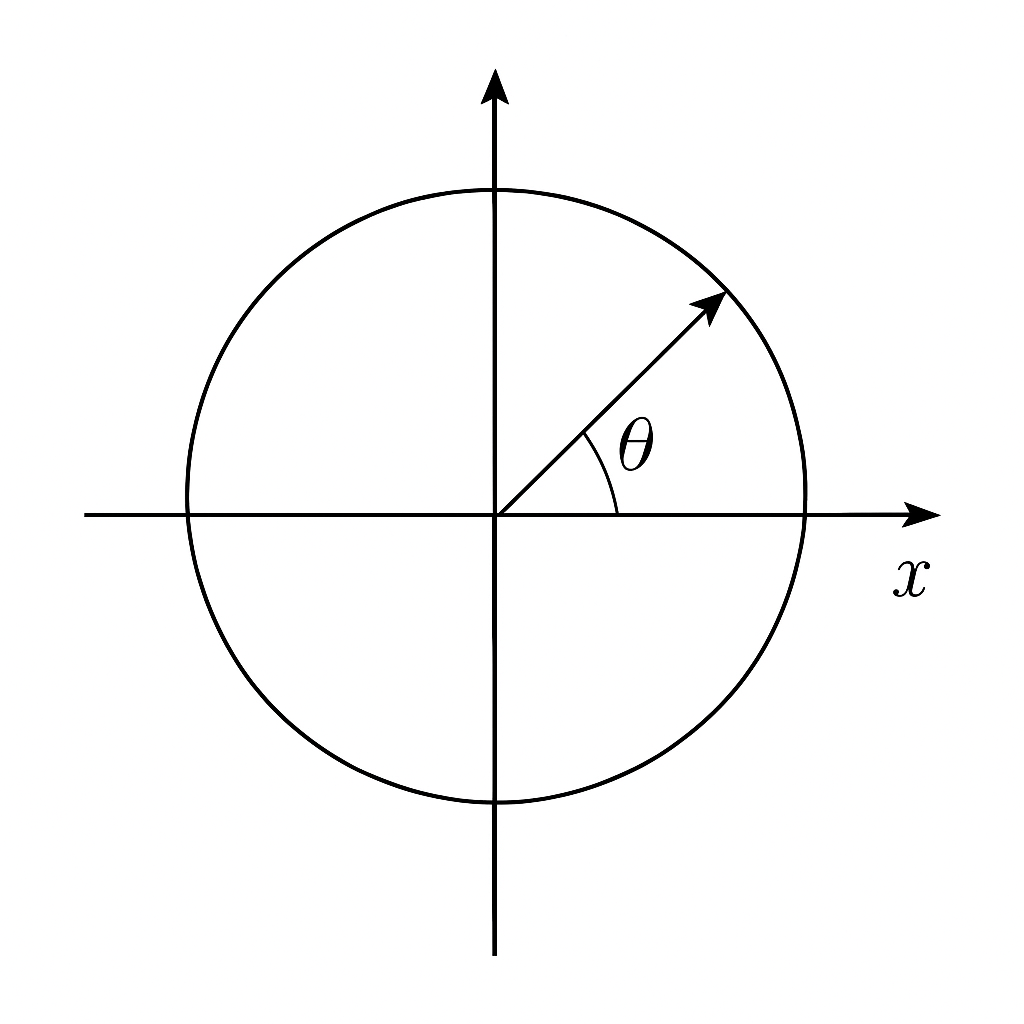
\includegraphics[width=\linewidth]{bilder/u1_kreis.png}
	\end{minipage}%
	\begin{minipage}{0.63\textwidth}
		Die Gruppe \(\mathrm{U(1)}\) kann man sich anschaulich als alle möglichen
		Drehungen auf einem Kreis vorstellen.  
		Jeder Punkt auf dem Kreis wird durch einen Winkel \(\theta\) beschrieben.  
		In der Quantenmechanik entspricht dies einer Phasenänderung der Wellenfunktion
		– der Abstand zum Ursprung bleibt immer gleich, nur die Richtung ändert sich.
	\end{minipage}
\end{tcolorbox}

\subsection{Elektroschwache Vereinheitlichung}


Die \textbf{elektroschwache Theorie}\index{Elektroschwache Theorie} beschreibt die Vereinigung der \textbf{elektromagnetischen Wechselwirkung}\index{Elektromagnetische Wechselwirkung} und der \textbf{schwachen Wechselwirkung}\index{Schwache Wechselwirkung} in einem gemeinsamen theoretischen Rahmen.  
Sie wurde Ende der 1960er Jahre von \textbf{Sheldon Glashow}\index{Glashow, Sheldon}, \textbf{Abdus Salam}\index{Salam, Abdus} und \textbf{Steven Weinberg}\index{Weinberg, Steven} entwickelt und bildet einen zentralen Bestandteil des \textbf{Standardmodells der Teilchenphysik}\index{Standardmodell der Teilchenphysik}.  
Für diese Leistung erhielten sie 1979 den \textbf{Nobelpreis für Physik}\index{Nobelpreis für Physik}.

Mathematisch basiert die elektroschwache Theorie auf der Symmetriegruppe \(\mathrm{SU(2)} \times \mathrm{U(1)}\)\index{SU(2)}\index{U(1)}.  
Die \(\mathrm{SU(2)}\)-Symmetrie beschreibt die schwache Wechselwirkung mit ihren drei Eichbosonen \(W^1, W^2, W^3\)\index{Eichboson}, während die \(\mathrm{U(1)}\)-Symmetrie den elektromagnetischen Anteil repräsentiert.  
Durch eine Mischung (\emph{Weinberg-Winkel}\index{Weinberg-Winkel}) der Felder \(W^3\) und \(B\) (dem U(1)-Boson) entstehen das masselose \textbf{Photon}\index{Photon} und das neutrale \textbf{\(Z^0\)-Boson}\index{Z-Boson}.

Die elektroschwache Symmetrie wird durch den \textbf{Higgs-Mechanismus}\index{Higgs-Mechanismus} spontan gebrochen.  
Dadurch erhalten die \(W^\pm\)- und \(Z^0\)-Bosonen\index{W-Boson}\index{Z-Boson} eine Masse, während das Photon masselos bleibt.  
Diese Eigenschaft ist ein direkter Ausdruck der verbleibenden ungebrochenen U(1)-Symmetrie\index{U(1)-Eichsymmetrie} der Elektrodynamik.

Die experimentelle Bestätigung der elektroschwachen Theorie gelang Anfang der 1980er Jahre am CERN\index{CERN} durch den direkten Nachweis der \(W\)- und \(Z\)-Bosonen.  
Diese Entdeckung gilt als einer der größten Erfolge der modernen Teilchenphysik.
\vspace{1em}
\begin{tcolorbox}[didaktikbox, title=Vom \(W^3\) und \(B\) zum Photon]
	\label{box:weinberg_mischung}
	\small
	\begin{minipage}{0.35\textwidth}
		\centering
		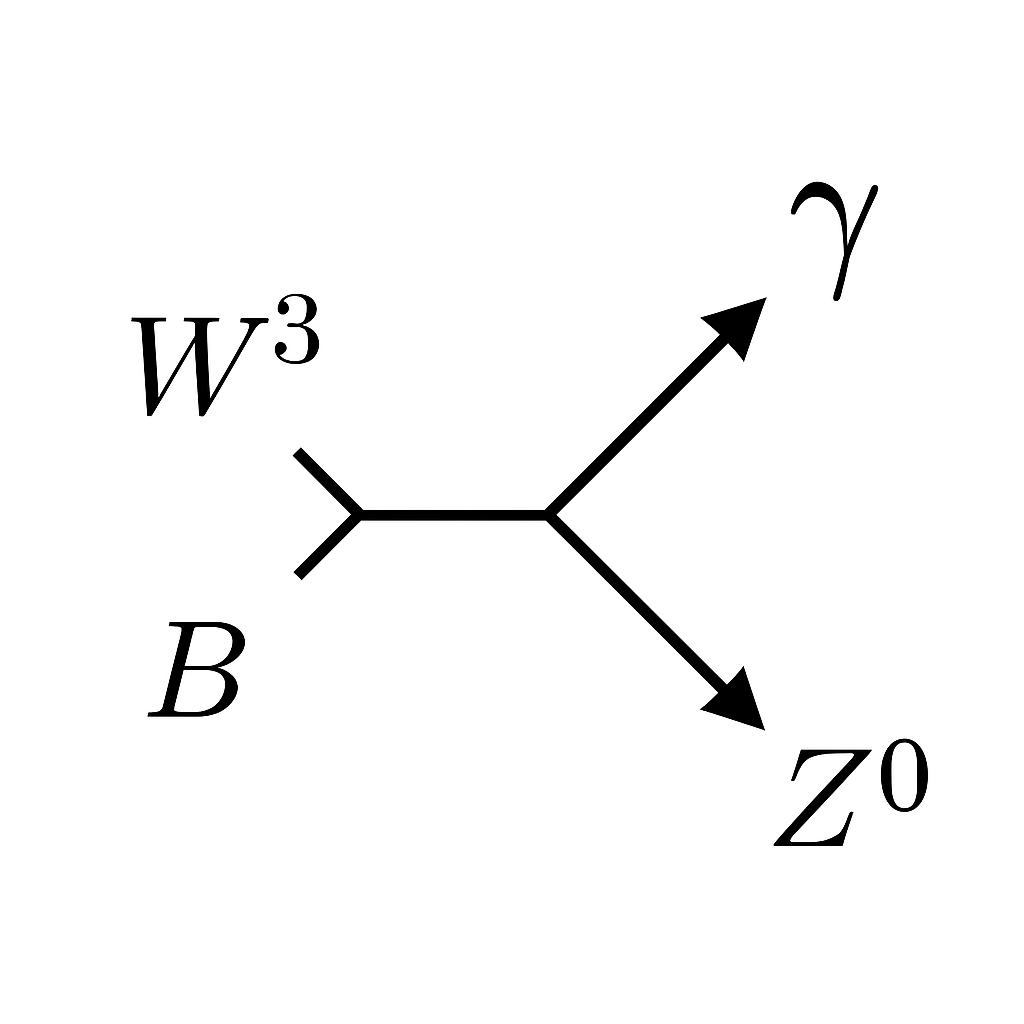
\includegraphics[width=\linewidth]{bilder/weinberg_mischung.png}
	\end{minipage}%
	\begin{minipage}{0.63\textwidth}
		In der elektroschwachen Theorie entstehen das \textbf{Photon} \(\gamma\) und das neutrale 
		\(\mathbf{Z^0}\)-Boson durch eine Mischung der Felder \(W^3\) und \(B\) 
		– beschrieben durch den \textbf{Weinberg-Winkel} \(\theta_W\).  
		\vspace{0.3em}
		
		Mathematisch gilt:
		\[
		\begin{aligned}
			\gamma &= \phantom{-}\cos\theta_W \, B + \sin\theta_W \, W^3 \\
			Z^0    &= -\sin\theta_W \, B + \cos\theta_W \, W^3
		\end{aligned}
		\]
		Diese Rotation der Felder erklärt, warum das Photon masselos bleibt, während 
		das \(Z^0\)-Boson eine Masse erhält.
	\end{minipage}
\end{tcolorbox}


\subsection{Warum ist das Photon masselos?}


Das \textbf{Photon}\index{Photon} ist im Rahmen des \textbf{Standardmodells der Teilchenphysik}\index{Standardmodell der Teilchenphysik} ein masseloses \textbf{Eichboson}\index{Eichboson} der elektromagnetischen Wechselwirkung.  
Seine Masselosigkeit ist eine direkte Folge der ungebrochenen \textbf{U(1)-Eichsymmetrie}\index{U(1)-Eichsymmetrie} in der \textbf{Quantenelektrodynamik (QED)}\index{Quantenelektrodynamik (QED)}.

Im \textbf{Higgs-Mechanismus}\index{Higgs-Mechanismus}, der in der elektroschwachen Theorie die \(W^\pm\)- und \(Z^0\)-Bosonen\index{W-Boson}\index{Z-Boson} mit Masse versieht, bleibt genau eine Eichsymmetrie ungebrochen: die U(1)-Symmetrie der Elektrodynamik.  
Das zugehörige Eichfeld wird als Photon identifiziert – und da ungebrochene Eichsymmetrien immer zu masselosen Austauschteilchen führen, besitzt das Photon keine Ruhemasse.

Mathematisch äußert sich dies darin, dass in der Lagrangedichte\index{Lagrangedichte} des elektromagnetischen Feldes kein Massenterm der Form \(\frac{1}{2} m^2 A_\mu A^\mu\) auftritt.  
Ein solcher Term würde die Eichinvarianz verletzen und ist daher verboten.

Die experimentellen Grenzen für eine eventuelle Photonenmasse sind extrem streng:  
Messungen setzen eine obere Schranke von weniger als \(10^{-18}\,\mathrm{eV}/c^2\)\index{Photonenmasse} fest.  
Praktisch ist das Photon daher perfekt masselos – eine Eigenschaft, die für die unendliche Reichweite\index{Reichweite elektromagnetischer Wechselwirkung} der elektromagnetischen Kraft entscheidend ist.
\vspace{1em}
\begin{tcolorbox}[hinweisbox, title=Masselosigkeit und Reichweite]
	\label{box:reichweite_masselos}
	\small
	Die Reichweite einer fundamentalen Wechselwirkung hängt direkt von der Masse ihres Austauschteilchens ab.  
	\begin{itemize}
		\item \textbf{Masselose Austauschteilchen} (z.\,B. Photonen) vermitteln Kräfte mit unbegrenzter Reichweite.  
		\item \textbf{Massive Austauschteilchen} (z.\,B. \(W^\pm\)- und \(Z^0\)-Bosonen) vermitteln Kräfte mit endlicher Reichweite, die durch die \emph{Compton-Wellenlänge} \(\lambda_C = \hbar/(mc)\) bestimmt wird.
	\end{itemize}
	Für das Photon folgt aus seiner Masselosigkeit die unendliche Reichweite der elektromagnetischen Wechselwirkung.
\end{tcolorbox}
\vspace{1em}
\begin{tcolorbox}[physikbox, title=Masseloses Photon und Spinwirkung über große Distanzen]
	\label{box:photon_spin_reichweite}
	\small
	Ein masseloses Photon besitzt keine Reichweitenbegrenzung für die Vermittlung seiner quantisierten Eigenschaften.  
	Das hat zwei wesentliche Konsequenzen:
	\begin{itemize}
		\item \textbf{Unendliche Reichweite der Wechselwirkung:} Die elektromagnetische Kraft wirkt prinzipiell über beliebige Entfernungen.
		\item \textbf{Erhalt der Spinrichtung (Polarisation):} Da das Photon masselos ist und sich mit Lichtgeschwindigkeit bewegt, bleibt seine Spin- bzw. Polarisationsausrichtung auch über kosmologische Distanzen erhalten. 
	\end{itemize}
	In verschränkten Quantenzuständen bedeutet dies, dass die Korrelation der Polarisation zweier Photonen selbst dann messbar bleibt, wenn sie weit voneinander entfernt sind – eine Folge der Kombination von Masselosigkeit und quantenmechanischer Verschränkung.
\end{tcolorbox}


\subsection{Vergleich mit anderen Eichbosonen}

Im \textbf{Standardmodell der Teilchenphysik}\index{Standardmodell der Teilchenphysik} existieren mehrere \textbf{Eichbosonen}\index{Eichboson}, die fundamentale Wechselwirkungen vermitteln.  
Das \textbf{Photon}\index{Photon} unterscheidet sich von ihnen in wesentlichen Eigenschaften:

\begin{itemize}
	\item \textbf{Photon (QED):} Masselos, Spin \(1\), vermittelt die \textbf{elektromagnetische Wechselwirkung}\index{Elektromagnetische Wechselwirkung}.  
	Reichweite: unendlich.
	
	\item \(\mathbf{W^\pm}\)- und \(\mathbf{Z^0}\)-\textbf{Bosonen} (elektroschwache Theorie)\index{W-Boson}\index{Z-Boson}:  
	Spin \(1\), besitzen hohe Masse (\(\approx 80{-}91\,\mathrm{GeV}/c^2\)), Reichweite: etwa \(10^{-18}\,\mathrm{m}\).  
	Vermitteln die \textbf{schwache Wechselwirkung}\index{Schwache Wechselwirkung}.
	
	\item \textbf{Gluonen} (QCD)\index{Gluon}:  
	Spin \(1\), formal masselos, vermitteln die \textbf{starke Wechselwirkung}\index{Starke Wechselwirkung}.  
	Reichweite jedoch effektiv stark begrenzt durch \textbf{Confinement}\index{Confinement} – Gluonen treten nicht als freie Teilchen auf.
	
	\item \textbf{Graviton}\index{Graviton} (hypothetisch):  
	Spin \(2\), masselos, würde die Gravitation vermitteln.  
	Noch nicht experimentell nachgewiesen.
\end{itemize}

Der entscheidende Unterschied:  
Nur das Photon tritt als frei messbares, masseloses Austauschteilchen mit unbegrenzter Reichweite auf.  
W- und Z-Bosonen sind massiv und daher kurzreichweitig, Gluonen sind zwar masselos, aber durch Confinement in gebundenen Zuständen gefangen.
\vspace{1em}
\begin{tcolorbox}[hinweisbox, title=Vergleich der Eichbosonen]
	\label{box:eichbosonen_vergleich}
	\small
	
	\resizebox{\linewidth}{!}{%
		\begin{tabular}{lcccc}
			\textbf{Teilchen} & \textbf{Spin} & \textbf{Masse} & \textbf{Reichweite} & \textbf{Wechselwirkung} \\
			\hline
			Photon & 1 & 0 & unendlich & elektromagnetisch \\
			\(W^\pm\) & 1 & \(\approx 80\,\mathrm{GeV}/c^2\) & \(10^{-18}\,\mathrm{m}\) & schwach \\
			\(Z^0\) & 1 & \(\approx 91\,\mathrm{GeV}/c^2\) & \(10^{-18}\,\mathrm{m}\) & schwach \\
			Gluon & 1 & 0 & \emph{effektiv kurz} & stark (Confinement) \\
			Graviton (hyp.) & 2 & 0 & unendlich & Gravitation \\
		\end{tabular}%
	}
	
\end{tcolorbox}




\subsection{Offene Fragen und Erweiterungen}

Trotz des Erfolgs des \textbf{Standardmodells der Teilchenphysik}\index{Standardmodell der Teilchenphysik} bleiben zentrale Fragen unbeantwortet, die auch das \textbf{Photon}\index{Photon} betreffen oder seinen theoretischen Rahmen erweitern könnten:

\begin{itemize}
	\item \textbf{Photonenmasse}\index{Photonenmasse}:  
	Experimentell gilt das Photon als masselos, doch ist nicht ausgeschlossen, dass es eine extrem kleine, bislang unmessbare Masse besitzt.  
	Verbesserte Messungen könnten diese Grenze weiter einschränken oder – überraschend – eine endliche Masse nachweisen.
	
	\item \textbf{Wechselwirkung mit Dunkler Materie}\index{Dunkle Materie}:  
	Ob Photonen in irgendeiner Form mit Dunkler Materie koppeln, ist unbekannt.  
	Direkte und indirekte Suchmethoden könnten hier in Zukunft Hinweise liefern.
	
	\item \textbf{Vereinheitlichte Theorien}\index{Vereinheitlichte Theorie}:  
	In Theorien jenseits des Standardmodells – etwa \textbf{Große Vereinheitlichung (GUT)}\index{Große Vereinheitlichung} oder \textbf{String\-theorien}\index{Stringtheorie} – ist das Photon Teil eines größeren Symmetriegefüges.  
	Diese Modelle könnten neue Eigenschaften oder Partnerteilchen vorhersagen.
	
	\item \textbf{Quantengravitation}\index{Quantengravitation}:  
	Eine konsistente Theorie, die die Gravitation mit den Quantenfeldern der Teilchenphysik verbindet, fehlt bislang.  
	Die Wechselwirkung des Photons mit hypothetischen \textbf{Gravitonen}\index{Graviton} oder der Struktur der Raumzeit auf kleinster Skala ist weitgehend unerforscht.
	
	\item \textbf{Neue Symmetrien oder Teilchen}:  
	Erweiterungen des Standardmodells könnten zusätzliche Eichbosonen oder Symmetrien beinhalten, die Einfluss auf die Rolle des Photons haben.
\end{itemize}

Die Beantwortung dieser Fragen erfordert eine Kombination aus präzisen Experimenten, neuen Beobachtungstechnologien und theoretischen Durchbrüchen.  
Das Photon bleibt damit nicht nur ein zentrales Werkzeug der Physik, sondern auch ein Schlüssel zu möglichen neuen physikalischen Welten.
\subsection{Fazit}
\subsubsection*{Das Photon – Teilchen, Welle und Fenster zur Zukunft}
\phantomsection
Das \textbf{Photon}\index{Photon} hat in der Geschichte der Physik eine einzigartige Rolle gespielt:  
Es war der Schlüssel zur Entstehung der Quantentheorie, der Ausgangspunkt für die Entwicklung der \textbf{Quantenelektrodynamik (QED)}\index{Quantenelektrodynamik (QED)} und bleibt bis heute ein unverzichtbares Werkzeug der experimentellen und theoretischen Forschung.

Vom \textbf{Photoeffekt}\index{Photoeffekt} über die \textbf{Compton-Streuung}\index{Compton-Streuung} bis hin zu modernen Anwendungen wie \textbf{Quantenkommunikation}\index{Quantenkommunikation} und \textbf{Photonik}\index{Photonik} hat das Photon nicht nur unsere physikalischen Modelle geprägt, sondern auch Technologien ermöglicht, die unseren Alltag verändern.

Im Rahmen des \textbf{Standardmodells der Teilchenphysik}\index{Standardmodell der Teilchenphysik} steht das Photon für eine ungebrochene \textbf{U(1)-Eichsymmetrie}\index{U(1)-Eichsymmetrie} – eine mathematische Eleganz, die sich in seiner Masselosigkeit und unendlichen Reichweite widerspiegelt.  
Gleichzeitig zeigt der Blick auf offene Fragen, dass wir vom vollständigen Verständnis noch weit entfernt sind.
\newpage
\noindent
Das Photon verbindet fundamentale Eigenschaften der Natur:
\begin{itemize}
	\item \textbf{Welle und Teilchen} in einer einzigen Quantenbeschreibung.
	\item \textbf{Masseloser Bote} mit unendlicher Reichweite.
	\item \textbf{Präzise Messsonde} in Astronomie, Teilchenphysik und Quantenoptik.
	\item \textbf{Schlüsselakteur} in künftigen Technologien wie Quantencomputern und photonischen Schaltkreisen.
\end{itemize}

Seine Doppelrolle als theoretisches Fundament und praktisches Werkzeug macht das Photon zu einem der faszinierendsten Objekte der Physik.  
Es ist nicht nur ein Bestandteil unseres physikalischen Weltbildes, sondern auch ein Tor zu noch unbekannten Aspekten des Universums – ein Tor, das wir in den kommenden Jahrzehnten weiter aufstoßen werden.



Auch wenn das Photon im Standardmodell in einer klaren und konsistenten Rolle erscheint, 
bleibt es zugleich ein Symbol für die Grenzen dieser Theorie.  
Um diese Doppelfunktion hervorzuheben – als Fundament und als Brücke zu neuer Physik – 
fassen wir die wichtigsten Erkenntnisse didaktisch zusammen und werfen anschließend 
einen spekulativen Blick in die Zukunft.
\vspace{1em}
\begin{tcolorbox}[didaktikbox, title=Didaktischer Abschluss: Das Photon im Standardmodell]
	\label{box:didaktik_kapVIII}
	Das Photon ist nicht nur ein Werkzeug der Quantenoptik und modernen Technologie, 
	sondern auch eine Schlüsselfigur im theoretischen Fundament der Physik.  
	
	\medskip
	\textbf{Kernbotschaft:}  
	Seine Rolle als masseloses Eichboson der ungebrochenen U(1)-Symmetrie verbindet mathematische Eleganz, 
	experimentelle Präzision und kosmische Reichweite.  
	Damit steht das Photon exemplarisch für die Stärke – aber auch für die Grenzen – des Standardmodells.
\end{tcolorbox}
\vspace{1em}
\begin{tcolorbox}[hypobox, title={Was wäre, wenn das Standardmodell nur ein Zwischenschritt wäre?}]
	\label{Merksatz zum Photon}
	Ein Gedankenspiel:
	\begin{itemize}
		\item Wenn Photonen mit Dunkler Materie wechselwirken könnten, würde das unser Verständnis von Kosmologie revolutionieren.  
		\item Ein Nachweis winziger Photonenmassen würde die Struktur der Elektrodynamik grundlegend ändern.  
		\item Neue Symmetrien oder verborgene Partnerteilchen des Photons könnten in einer erweiterten Theorie jenseits des Standardmodells auftauchen.  
		\item Vielleicht ist das Photon sogar der Schlüssel zur Verbindung von Quantenfeldtheorie und Gravitation.  
	\end{itemize}
	
	\medskip
	Solche spekulativen Perspektiven führen über das Standardmodell hinaus – und öffnen die Tür 
	zu einem künftigen Kapitel über \emph{neue Physik}.
\end{tcolorbox}

	
	% Anhänge
	
\cleardoublepage
\appendix
\renewcommand{\thechapter}{A}

\renewcommand{\thesection}{\Alph{chapter}.\arabic{section}}

\chapter{Mathematische Hintergründe und Herleitungen}
\label{anhangA}

In diesem Anhang werden die im Haupttext angesprochenen physikalischen Konzepte
formal und mathematisch vertieft. Ziel ist es, die didaktische Lesbarkeit der
Kapitel nicht zu beeinträchtigen und zugleich interessierten Lesern die
vollständigen Herleitungen zugänglich zu machen. 

Die Abschnitte sind thematisch nach den zentralen Eigenschaften des Photons
gegliedert, darunter Energie-Impuls-Relation, Massehypothese, Helizität und
Polarisation.\index{Photon!Eigenschaften} Auf diese Weise bildet der Anhang eine Brücke zwischen den
intuitiven Erklärungen im Haupttext und der mathematischen Strenge der
Quantenfeldtheorie.

%\section{Kapitel I}
\phantomsection
\section{Energie- und Impulsrelation des Photons}\index{Energie-Impuls-Relation!Photon}
\label{anhangA:energie_impuls}

In diesem Abschnitt wird formal hergeleitet, warum ein Photon die Energie
\[
E = h f
\]
und den Impuls
\[
p = \frac{h}{\lambda}
\]
besitzt. Ausgangspunkt sind die Maxwell-Gleichungen und deren Wellengleichung.
Über den Poynting-Vektor und die Energiedichte des elektromagnetischen Feldes
wird gezeigt, dass die Quantisierung der Felder zu diskreten Energieportionen
führt. Diese Herleitung ergänzt die intuitive Darstellung im Haupttext
(Kapitel~I).

\section{Das elektromagnetische Feld in der relativistischen Formulierung}\index{Elektromagnetisches Feld!relativistische Formulierung}\index{Feldstärketensor}\index{Lagrangedichte}
\label{anhangA:feldtheorie}

Hier erfolgt die Einführung in die formale Beschreibung des elektromagnetischen
Feldes:

\begin{itemize}
	\item Viererpotential $A^\mu = (\phi, \vec{A})$
	\item Feldstärketensor $F^{\mu\nu} = \partial^\mu A^\nu - \partial^\nu A^\mu$
	\item Antisymmetrie-Eigenschaft $F^{\mu\nu} = -F^{\nu\mu}$
	\item Lagrangedichte
	\[
	\mathcal{L} = -\frac{1}{4} F_{\mu\nu}F^{\mu\nu}
	\]
	\item Zusammenhang zur Quantisierung: Photon als Eichboson des $U(1)$
	Elektromagnetismus
\end{itemize}

Dies liefert den mathematischen Unterbau zur Aussage im Haupttext, dass
Photonen „Anregungen des elektromagnetischen Feldes“ sind.

\section{Formale Beschreibung verschränkter Photonen}\index{Photonen!Verschränkung}\index{Dirac-Notation}\index{SPDC (Spontane parametrische Fluoreszenz)}
\label{anhangA:verschr}

Die im Haupttext (Kapitel~I) dargestellten Experimente zur Erzeugung
verschränkter Photonenpaare (SPDC) lassen sich formal in der
Dirac-Notation beschreiben. Ein typisches verschränktes
Polarisations-Zustandspaar lautet:

\[
|\psi\rangle = \frac{1}{\sqrt{2}}\big( |H\rangle_A \otimes |V\rangle_B +
|V\rangle_A \otimes |H\rangle_B \big)
\]

\begin{itemize}
	\item $|H\rangle$: horizontal polarisierter Zustand
	\item $|V\rangle$: vertikal polarisierter Zustand
	\item Indizes $A, B$: die beiden Photonen
\end{itemize}

Dieser Formalismus macht die im Experiment beobachteten Korrelationen
transparent und zeigt, warum klassische Modelle mit verborgenen Variablen
nicht ausreichen.

%Kapitel II
%\section{Kapitel II}
\section{Herleitung des Rayleigh-Jeans-Gesetzes}\index{Rayleigh-Jeans-Gesetz!Herleitung}\index{Rayleigh, Lord}\index{Jeans, James}\index{Ultraviolett-Katastrophe}
\label{anhangA:rayleigh}

Das Rayleigh-Jeans-Gesetz ergibt sich, wenn man die elektromagnetischen
Moden in einem Hohlraum wie harmonische Oszillatoren behandelt:

\begin{enumerate}
	\item Man zählt die Anzahl der stehenden Wellen im Würfelvolumen $V$.
	\item Jede Mode besitzt zwei Polarisationsrichtungen.
	\item Nach dem Ausrüstungsprinzip der klassischen Thermodynamik trägt
	jede Freiheitsgrad im Gleichgewicht die mittlere Energie $kT$.
\end{enumerate}

Die Anzahl der Moden zwischen den Frequenzen $\nu$ und $\nu + d\nu$ ist
\[
g(\nu)\, d\nu = \frac{8\pi V \nu^2}{c^3}\, d\nu.
\]

Multipliziert mit $kT$ ergibt dies die spektrale Energiedichte
\[
u(\nu, T) = \frac{8\pi \nu^2}{c^3}\, kT,
\]
die in Wellenlängenform $u(\lambda, T) = \tfrac{8\pi kT}{\lambda^4}$ lautet.
Das Gesetz stimmt bei langen Wellenlängen, divergiert jedoch für
$\lambda \to 0$ – die \emph{Ultraviolett-Katastrophe}.

\section{Das Wiensche Strahlungsgesetz}\index{Wiensches Strahlungsgesetz}\index{Wien, Wilhelm}
\label{anhangA:wien}

Wilhelm Wien leitete 1896 eine Näherung für die Schwarzkörperstrahlung her.
Die Argumentation beruhte auf:

\begin{itemize}
	\item Thermodynamischen Überlegungen: Adiabatische Kompression eines
	Hohlraums verschiebt das Strahlungsspektrum.
	\item Dimensionsanalyse: Die Intensität hängt von $T$ und $\lambda$ ab
	und muss die korrekten Einheiten haben.
\end{itemize}

Das Resultat war
\[
u(\lambda, T) = \frac{c_1}{\lambda^5}\,
\exp\!\left(-\frac{c_2}{\lambda T}\right),
\]
mit Konstanten $c_1, c_2$, die erst durch Plancks Ansatz vollständig
verstanden wurden. Das Wiensche Gesetz stimmt im UV-Bereich,
versagt jedoch bei langen Wellenlängen.

\section{Herleitung des Planckschen Strahlungsgesetzes}\index{Plancksches Strahlungsgesetz!Herleitung}\index{Planck, Max}
\label{anhangA:planck}

Planck kombinierte die Grenzgesetze von Rayleigh-Jeans und Wien und
führte die Quantisierung der Energie ein:

\begin{itemize}
	\item Ein Oszillator kann nur Energien $E_n = nh\nu$ annehmen.
	\item Die Besetzungswahrscheinlichkeit folgt der Boltzmann-Verteilung.
\end{itemize}

Die mittlere Energie pro Oszillator lautet
\[
\langle E \rangle = \frac{h\nu}{e^{h\nu/kT} - 1}.
\]

Multipliziert mit der Modenzahl
$g(\nu)\, d\nu = \tfrac{8\pi V \nu^2}{c^3}\, d\nu$
ergibt dies die Strahlungsdichte
\[
u(\nu, T) = \frac{8\pi \nu^2}{c^3}\,
\frac{h\nu}{e^{h\nu/kT} - 1}.
\]

Dies ist das \textbf{Plancksche Strahlungsgesetz}, das für alle Frequenzen
mit dem Experiment übereinstimmt.

\section{Mathematische Beschreibung des Photoeffekts}\index{Photoeffekt!Mathematische Beschreibung}
\label{anhangA:photoeffekt}

Beim Photoeffekt absorbiert ein Elektron in einem Metall ein Photon
mit Energie $E_\gamma = h\nu$. Um das Elektron aus dem Metall zu lösen,
muss die \emph{Austrittsarbeit} $A$ überwunden werden. Die überschüssige
Energie geht in die kinetische Energie des Elektrons über:

\[
E_\text{kin} = h\nu - A.
\]

Daraus folgt eine \emph{Grenzfrequenz}
\[
\nu_\text{min} = \frac{A}{h},
\]
unterhalb derer keine Elektronen ausgelöst werden – unabhängig von der
Lichtintensität. Diese lineare Beziehung zwischen Elektronenenergie und
Lichtfrequenz wurde in Millikans Experimenten (1916) präzise bestätigt.\index{Millikan, Robert A.}
%\section{Kapitel III}
\section{Photonenimpuls}\index{Photon!Impuls}\index{Energie-Impuls-Relation}
\label{anhangA:impuls}

Der Impuls eines Photons lässt sich aus der relativistischen Energie-Impuls-Relation ableiten. Für beliebige Teilchen gilt
\[
E^2 = (pc)^2 + (m_0 c^2)^2 ,
\]
wobei $E$ die Energie, $p$ der Impuls, $c$ die Lichtgeschwindigkeit und $m_0$ die Ruhemasse ist.

\begin{itemize}
	\item Für masselose Teilchen ($m_0 = 0$) reduziert sich diese Gleichung zu
	\[
	E = p c.
	\]
	
	\item Für das Photon gilt zugleich die Quantisierungsbedingung
	\[
	E = h f = \frac{h c}{\lambda}.
	\]
	
	\item Setzt man beide Ausdrücke für $E$ gleich, folgt unmittelbar
	\[
	p = \frac{E}{c} = \frac{h}{\lambda}.
	\]
\end{itemize}

\noindent
Damit ist der Impuls eines Photons direkt an seine Wellenlänge gekoppelt. Diese Beziehung ist eine der zentralen Brücken zwischen Wellen- und Teilchenbeschreibung des Lichts.

\section{Energie-Impuls-Relation des Photons}\index{Photon!Massehypothese}\index{Photon!Masselosigkeit}\index{Energie-Impuls-Relation}
\label{anhangA:masse}

Für relativistische Teilchen gilt allgemein die Energie-Impuls-Relation:
\[
E^2 = (pc)^2 + (m c^2)^2.
\]

\begin{itemize}
	\item \textbf{Masseloses Photon:}  
	Setzt man $m=0$, so folgt unmittelbar:
	\[
	E = p c.
	\]
	Dies steht im Einklang mit den Relationen $E = h f$ und $p = h/\lambda$.
	
	\item \textbf{Hypothetisch massives Photon:}  
	Angenommen, das Photon hätte eine Ruhemasse $m_\gamma \neq 0$, so ergäbe sich:
	\[
	E^2 = (p c)^2 + (m_\gamma c^2)^2.
	\]
	Ein solches Photon würde sich stets langsamer als $c$ bewegen, und die Lichtgeschwindigkeit wäre nicht mehr universell konstant. 
	Bereits minimale Abweichungen von $m=0$ würden sich in Präzisionsexperimenten zeigen.
\end{itemize}

Experimentell konnte bisher nur eine obere Schranke für die Photonenmasse gesetzt werden. Aktuelle Grenzen liegen bei
\[
m_\gamma < 10^{-18}\,\text{eV}/c^2,
\]
was faktisch bedeutet, dass das Photon als masselos angesehen wird.

\section{Helizität des Photons}\index{Photon!Helizität}\index{Spin}
\label{anhangA:helizitaet}

Das Photon besitzt Spin $s=1$, doch aufgrund seiner Masselosigkeit sind nicht alle drei Spinprojektionen ($m_s=-1,0,+1$) physikalisch realisierbar. 

\begin{itemize}
	\item \textbf{Allgemeiner Spin-1-Zustand:}  
	Für massive Spin-1-Teilchen sind drei Polarisationszustände möglich, entsprechend den Projektionen $m_s=-1,0,+1$ auf die Bewegungsrichtung.
	
	\item \textbf{Masseloses Photon:}  
	Da das Photon keine Ruhemasse hat, existiert kein Ruhesystem, in dem man die Spinausrichtung unabhängig vom Bewegungsvektor definieren könnte.  
	Mathematisch erzwingt die Eichinvarianz der Maxwellgleichungen (bzw. des QED-Formalismus), dass die longitudinale Komponente ($m_s=0$) verschwindet.
	
	\item \textbf{Helizitätszustände:}  
	Übrig bleiben nur zwei mögliche Zustände:
	\begin{align*}
		\lambda& = +1 \quad \text{(Rechtsdrehung, Rechtspolarisation)}\\
		\lambda &= -1 \quad \text{(Linksdrehung, Linkspolarisation)}
	\end{align*}
	
	Diese werden als die beiden Helizitätszustände des Photons bezeichnet.
\end{itemize}

\noindent
Damit ist das Photon ein zweizuständiges masseloses Boson, dessen Freiheitsgrade vollständig durch die beiden möglichen Helizitäten beschrieben werden.

\section{Polarisation des Photons}\index{Photon!Polarisation}\index{Dirac-Notation}\index{Jones-Vektor}
\label{anhangA:polarisation}

Die Polarisation beschreibt die transversale Schwingungsrichtung des elektrischen Feldes eines Photons. Formal lässt sich dieser Freiheitsgrad auf zwei Arten darstellen:

\begin{itemize}
	\item \textbf{Dirac-Notation:}  
	In der Quantenmechanik werden Polarisationszustände als Basisvektoren in einem zweidimensionalen Hilbertraum notiert:  
	\[
	|H\rangle = \begin{pmatrix}1 \\ 0\end{pmatrix}, \qquad
	|V\rangle = \begin{pmatrix}0 \\ 1\end{pmatrix},
	\]
	wobei $|H\rangle$ für horizontale und $|V\rangle$ für vertikale Polarisation steht.  
	Beliebige Polarisationszustände lassen sich als Linearkombination schreiben:  
	\[
	|\psi\rangle = \alpha |H\rangle + \beta |V\rangle, \quad |\alpha|^2 + |\beta|^2 = 1.
	\]
	
	\item \textbf{Jones-Vektoren:}  
	In der klassischen Optik wird derselbe Zustand durch \emph{Jones-Vektoren} beschrieben:  
	\[
	\vec{E} = \begin{pmatrix} E_x \\ E_y \end{pmatrix},
	\]
	wobei $E_x$ und $E_y$ komplexe Amplituden der elektrischen Feldkomponenten in $x$- und $y$-Richtung sind.  
	Auch hier gilt: normiert man die Intensität, so entspricht dies der Normierung des Zustandsvektors in der Dirac-Notation.
\end{itemize}

\noindent
Beide Beschreibungen sind äquivalent – die Dirac-Notation betont den quantenmechanischen Zustandsraum, während die Jones-Vektoren die klassische elektromagnetische Wellenoptik widerspiegeln.  
Die Verknüpfung dieser Darstellungen ist in der Quantenoptik ein zentrales Werkzeug.
%\section{Kapitel IV}
\section{Herleitung der Einstein-Gleichung beim Photoeffekt}
\label{anhangA:photoeffekt}

Die Einstein-Gleichung\index{Einstein-Gleichung}\index{Photoeffekt}
\[
E_{\text{kin}} = h \nu - A
\]
ergibt sich aus einer einfachen Energiebilanz zwischen Photon\index{Photon} und Elektron\index{Elektron}.

\begin{enumerate}
	\item Ein Photon besitzt die Energie
	\[
	E_{\text{Photon}} = h \nu,
	\]
	wobei \( h \) das Plancksche Wirkungsquantum\index{Plancksches Wirkungsquantum}\index{Planck, Max} und \( \nu \) die Frequenz\index{Frequenz} des einfallenden Lichts ist.
	
	\item Um ein Elektron aus dem Metall zu lösen, muss die \textbf{Austrittsarbeit} \( A \)\index{Austrittsarbeit} überwunden werden. Diese entspricht der minimalen Bindungsenergie der Elektronen im Festkörper.
	
	\item Bleibt nach Überwindung von \( A \) Energie übrig, so erscheint sie als kinetische Energie\index{Kinetische Energie} des Elektrons:
	\[
	E_{\text{kin}} = E_{\text{Photon}} - A.
	\]
	
	\item Damit folgt direkt:
	\[
	E_{\text{kin}} = h \nu - A.
	\]
\end{enumerate}

\textbf{Bemerkung:}  
Wird zusätzlich eine Gegenspannung \( U \)\index{Gegenspannung} angelegt, so gilt
\[
eU = h \nu - A,
\]
wobei \( e \) die Elementarladung\index{Elementarladung} ist. Diese Form erlaubt eine direkte experimentelle Bestimmung von \( h \) durch Messung der Stoppspannung\index{Stoppspannung} als Funktion der Frequenz.

\section{Planck–Einstein-Beziehung \texorpdfstring{$E = h\nu$}{E = hν}}
\label{anhangA:planckEinstein}
\index{Planck–Einstein-Beziehung}

\textbf{Ziel.} Wir begründen, warum ein einzelnes Lichtquant (Photon) die Energie
\[
E = h\nu = \hbar \omega
\]
trägt.

\subsection*{Weg 1: Quantisierung der Normalmoden des elektromagnetischen Feldes.}
\phantomsection
Das freie elektromagnetische Feld\index{Elektromagnetisches Feld} in einem Volumen \(V\) lässt sich in ebene Normalmoden mit Kreisfrequenzen \(\omega_{\mathbf{k}}\) zerlegen. Jede Mode entspricht einem harmonischen Oszillator\index{Harmonischer Oszillator} mit Hamiltonoperator
\[
\hat H_{\mathbf{k}}=\hbar \omega_{\mathbf{k}}\!\left(\hat a_{\mathbf{k}}^\dagger \hat a_{\mathbf{k}}+\tfrac12\right).
\]
Die Eigenwerte sind \((n+\tfrac12)\hbar\omega_{\mathbf{k}}\), \(n\in \mathbb{N}_0\). 
Eine Anregung \(\Delta n = 1\) erhöht die Energie exakt um \(\Delta E = \hbar \omega\). 
Diese Energiezunahme identifizieren wir mit \emph{einem Photon} in dieser Mode:
\[
E_{\text{Photon}}=\hbar\omega=h\nu.
\]

\subsection*{Weg 2: Von Plancks Quantenhypothese zu Einsteins Lichtquant.}
\phantomsection
Planck\index{Planck, Max} postulierte 1900 für Materieoszillatoren diskrete Energien \(E_n=n h\nu\).
Einstein\index{Einstein, Albert} übertrug 1905 die Quantisierung auf das \emph{Strahlungsfeld} selbst: die Energie der Strahlung verhält sich, als wäre sie in räumlich lokalisierte \emph{Energiepakete} der Größe \(h\nu\) gebündelt. 
Nur so lassen sich u.\,a. Entropieeigenschaften Wiensches Strahlungsgesetz\index{Wiensches Strahlungsgesetz}) und der Photoeffekt konsistent erklären. 
Damit folgt für ein einzelnes Lichtquant:
\[
E_{\text{Photon}} = h\nu.
\]

\subsection*{Konsequenzen.}
\phantomsection
(i) Die Photonenenergie hängt \emph{nur} von der Frequenz ab (nicht von der Intensität\index{Intensität}). 
(ii) In Verbindung mit \(E_{\text{kin}}=h\nu-A\) erklärt dies die Grenzfrequenz\index{Grenzfrequenz} beim Photoeffekt. 
(iii) Zusammen mit der Feldquantisierung führt dies zu Teilchenzahloperator \(\hat N=\hat a^\dagger \hat a\)\index{Teilchenzahloperator} und einer klaren Zuweisung der Energie pro Photon.

\section{Herleitung der Stoppspannungsgleichung}
\label{anhangA:stoppspannung}

\textbf{Ziel.} Zusammenhang zwischen Photonenenergie, Austrittsarbeit und messbarer Gegenspannung \(U\).

\subsection*{Ausgangspunkt.}
\phantomsection
Die Energiebilanz beim Photoeffekt lautet
\[
E_{\text{Photon}} = h\nu = A + E_{\text{kin,max}}.
\]

\subsection*{Experimentelles Prinzip.}
\phantomsection
In einer Fotozelle\index{Fotozelle} wird zwischen Kathode\index{Kathode} und Anode\index{Anode} eine \emph{Gegenspannung} \(U\) angelegt.  
Elektronen mit kinetischer Energie \(E_{\text{kin}}\) müssen Arbeit \(eU\) verrichten, um die Anode zu erreichen.  
Bei der \textbf{Stoppspannung} \(U_0\)\index{Stoppspannung} ist die Energie gerade aufgebraucht:
\[
E_{\text{kin,max}} = eU_0.
\]

\subsection*{Herleitung.}
\phantomsection
Setzt man dies in die Energiebilanz ein:
\[
h\nu = A + eU_0,
\]
folgt unmittelbar:
\[
eU_0 = h\nu - A.
\]

\subsection*{Experimentelle Bedeutung.}
\phantomsection
- Der Graph \(U_0(\nu)\) ist eine Gerade mit Steigung \(h/e\).  
- Der Achsenabschnitt liefert die materialabhängige Austrittsarbeit \(A\).  
- Millikan\index{Millikan, Robert} bestimmte damit 1916 den Wert des Planckschen Wirkungsquantums mit hoher Genauigkeit – und bestätigte Einsteins Hypothese experimentell.

\subsection*{Konsequenz.}
\phantomsection
Die Stoppspannung erlaubt eine direkte Messung fundamentaler Naturkonstanten, ohne dass Intensität oder Anzahl der Photonen eine Rolle spielen.

\section{Die Austrittsarbeit}
\label{anhangA:austrittsarbeit}

Die \textbf{Austrittsarbeit} \( A \) ist die Mindestenergie, die notwendig ist, um ein Elektron aus einem Metall zu lösen. 
Sie hängt vom Material und der elektronischen Struktur der Oberfläche ab. 

\textbf{Formale Definition:}
\[
A = E_{\text{Fermi}} + E_{\text{Bindung}} - E_{\text{Vakuum}}
\]
wobei \( E_{\text{Vakuum}} \) das Energieniveau eines Elektrons im Vakuum darstellt.

\textbf{Typische Werte:}
\begin{itemize}
	\item Alkalimetalle (z.\,B. Cäsium, Kalium)
	\item Übergangsmetalle (z.\,B. Eisen, Kupfer)
	\item Edelmetalle (z.\,B. Platin)
\end{itemize}

Die Austrittsarbeit erklärt, warum nur Photonen oberhalb einer \emph{Grenzfrequenz} \( \nu_0 = A/h \) Elektronen freisetzen können. 
Sie ist eine materialspezifische Größe und kann durch Oberflächenzustand, Temperatur oder Beschichtung variieren.

\section{Herleitung der Compton-Formel}
\label{anhangA:comptonHerleitung}

Die Herleitung der \textbf{Compton-Formel}\index{Compton-Formel} basiert auf Energie- und Impulserhaltung\index{Impulserhaltung} beim Stoß eines Photons mit einem ruhenden Elektron. 

\textbf{Ausgangssituation:}
\begin{itemize}
	\item Ein Photon mit Wellenlänge \( \lambda \) trifft auf ein Elektron in Ruhe.
	\item Nach dem Stoß hat das Photon die Wellenlänge \( \lambda' \) und wird um den Winkel \( \theta \) abgelenkt.
	\item Das Elektron erhält einen Rückstoßimpuls \( \vec{p}_e \).
\end{itemize}

\textbf{Erhaltungssätze:}
\begin{align*}
	E_\gamma + m_e c^2 &= E'_\gamma + E_e \\
	\vec{p}_\gamma &= \vec{p'}_\gamma + \vec{p}_e
\end{align*}
mit
\[
E_\gamma = \frac{hc}{\lambda}, \quad 
E'_\gamma = \frac{hc}{\lambda'}, \quad 
p_\gamma = \frac{h}{\lambda}, \quad 
E_e^2 = (p_e c)^2 + (m_e c^2)^2.
\]

\textbf{Ergebnis:}
\[
\Delta \lambda = \lambda' - \lambda 
= \frac{h}{m_e c}(1 - \cos \theta).
\]

Diese Verschiebung ist unabhängig von der Photonenenergie und hängt nur vom Streuwinkel ab. Der Faktor
\[
\lambda_C = \frac{h}{m_e c} \approx 2{,}43 \cdot 10^{-12}\,\mathrm{m}
\]
wird als \textbf{Compton-Wellenlänge} des Elektrons\index{Compton-Wellenlänge}\index{Compton, Arthur} bezeichnet.

\section{Der Doppelspalt im quantenmechanischen Formalismus}
\label{anhangA:doppelspalt}

Der Doppelspaltversuch\index{Doppelspaltversuch} mit einzelnen Photonen lässt sich nur mit Hilfe der Quantenmechanik\index{Quantenmechanik} verstehen. 
Im Gegensatz zur klassischen Wellentheorie\index{Wellentheorie} oder Teilchenmechanik\index{Teilchenmechanik} betrachtet man die \textbf{Wellenfunktion}\index{Wellenfunktion} 
eines Photons und deren Überlagerung.

\textbf{Superpositionsprinzip:}\index{Superpositionsprinzip}  
Treffen zwei mögliche Wege \( W_1 \) und \( W_2 \) auf, so gilt für die Gesamtamplitude:
\[
\Psi_{\text{gesamt}} = \Psi_{1} + \Psi_{2}.
\]

\textbf{Darstellung in der Dirac-Notation:}\index{Dirac-Notation}  
Sei \(|1\rangle\) der Zustand „Photon geht durch Spalt 1“ und \(|2\rangle\) der Zustand „Photon geht durch Spalt 2“.  
Ohne Messung des Weges gilt:
\[
|\psi\rangle = \frac{1}{\sqrt{2}} \left( |1\rangle + |2\rangle \right).
\]

\section{Antibunching und die Korrelationsfunktion}
\label{anhangA:antibunching}

Das Phänomen des \textbf{Antibunching}\index{Antibunching} zeigt, dass Photonen \emph{einzeln} emittiert werden. 
Mathematisch wird dies mit der Korrelationsfunktion zweiter Ordnung\index{Korrelationsfunktion} beschrieben.

\textbf{Definition:}
\[
g^{(2)}(\tau) = \frac{\langle I(t) \, I(t+\tau) \rangle}{\langle I(t) \rangle^2},
\]
wobei \( I(t) \) die Intensität (bzw. Zählrate) am Detektor ist und \(\tau\) die Zeitverzögerung zwischen zwei Messungen.

\textbf{Antibunching:}
Bei einer idealen Einzelphotonenquelle\index{Einzelphotonenquelle} findet man:
\[
g^{(2)}(0) = 0.
\]

\textbf{Physikalische Konsequenz:}
- Antibunching widerspricht jeder klassischen Wellenvorstellung.  
- Es zeigt die \textbf{Unteilbarkeit des Photons}: entweder wird es hier oder dort nachgewiesen – aber niemals gleichzeitig an zwei Orten.  
- Damit ist Antibunching ein direkter Beweis für die Quantennatur des Lichts.

\section{Hong--Ou--Mandel-Interferenz\newline
	 am Strahlteiler}
\label{anhangA:HOM}

Der \textbf{Hong--Ou--Mandel (HOM)-Effekt}\index{Hong-Ou-Mandel-Effekt}\index{Hong, Chung-ki}\index{Mandel, Leonard} beschreibt die Zwei-Pho\-tonen-Interferenz\index{Zwei-Photonen-Interferenz} identischer Photonen an einem 50:50-Strahlteiler.\index{Strahlteiler}
Bei perfekter Ununterscheidbarkeit\index{Ununterscheidbarkeit von Photonen} verschwinden Koinzidenzen an den beiden Ausgängen (``HOM-Dip''\index{HOM-Dip}).

\subsection*{Strahlteiler-Transformation (Heisenberg-Bild).}\index{Heisenberg-Bild}
\phantomsection
Für die Eingangsmoden \(\hat a,\hat b\) und Ausgangsmoden \(\hat c,\hat d\) eines verlustfreien 50:50-Strahlteilers wählen wir die unitäre Transformation
\[
\begin{pmatrix}
	\hat c \\ \hat d
\end{pmatrix}
= \frac{1}{\sqrt{2}}
\begin{pmatrix}
	1 & i \\
	i & 1
\end{pmatrix}
\begin{pmatrix}
	\hat a \\ \hat b
\end{pmatrix},
\qquad
\begin{pmatrix}
	\hat a \\ \hat b
\end{pmatrix}
= \frac{1}{\sqrt{2}}
\begin{pmatrix}
	1 & -i \\
	-i & 1
\end{pmatrix}
\begin{pmatrix}
	\hat c \\ \hat d
\end{pmatrix}.
\]
Für die Erzeugungsoperatoren gilt entsprechend
\[
\hat a^\dagger=\frac{\hat c^\dagger - i \hat d^\dagger}{\sqrt{2}},
\qquad
\hat b^\dagger=\frac{-i\,\hat c^\dagger + \hat d^\dagger}{\sqrt{2}}.
\]

\subsection*{Eingangszustand und Ausgangszustand.}
\phantomsection
Zwei einzelne Photonen, eins in jeder Eingangs­mode,
\(|\psi_{\text{in}}\rangle=\hat a^\dagger \hat b^\dagger |0\rangle\),
werden zu
\[
|\psi_{\text{out}}\rangle
= \hat a^\dagger \hat b^\dagger |0\rangle
= \frac{1}{2}\,(\hat c^\dagger - i \hat d^\dagger)(-i\,\hat c^\dagger + \hat d^\dagger)\,|0\rangle
= -\frac{i}{2}\!\left(\hat c^{\dagger 2}+\hat d^{\dagger 2}\right)|0\rangle.
\]
Da \(\hat c^\dagger \hat d^\dagger\)-Terme sich exakt auslöschen, enthält der Ausgangszustand \emph{keine} \(|1_c,1_d\rangle\)-Komponente (keine Koinzidenz). Nach Normierung ergibt sich äquivalent
\[
|\psi_{\text{out}}\rangle
\propto |2_c,0_d\rangle \,\pm\, |0_c,2_d\rangle,
\]
wobei das relative Vorzeichen nur von der Phasenkonvention des Strahlteilers abhängt, die Physik (Verschwinden der Koinzidenzen) jedoch identisch bleibt.

\subsection*{Unvollständige Überlappung und HOM-Dip.}
\phantomsection
Reale Photonen sind zeitlich/spektral/polarisatorisch endliche Wellenpakete. Sei
\(\Lambda(\tau)=\int\!dt\, f_a(t)\,f_b^*(t+\tau)\)
die (komplexe) Überlappungsintegral der zeitlichen Moden (Verzögerung \(\tau\)).
Dann ist die Koinzidenzwahrscheinlichkeit an den Ausgängen
\[
P_{\text{coinc}}(\tau)=\frac{1}{2}\Bigl(1-|\Lambda(\tau)|^2\Bigr).
\]
Für perfekt überlappende, ununterscheidbare Photonen gilt \(|\Lambda(0)|=1\Rightarrow P_{\text{coinc}}(0)=0\).
Für zwei gaussförmige Wellenpakete mit Kohärenzzeit \(\tau_c\) ist
\(|\Lambda(\tau)|^2=\exp[-(\tau/\tau_c)^2]\),
sodass
\[
P_{\text{coinc}}(\tau)=\tfrac{1}{2}\Bigl(1-e^{-(\tau/\tau_c)^2}\Bigr)
\]
den charakteristischen \emph{HOM-Dip} zeigt.

\subsection*{Einfluss von Ununterscheidbarkeit.}
\phantomsection
Jede Unterscheidbarkeit (Polarisationswinkel \(\Delta\phi\), spektrale oder räumliche Modenfehler) reduziert die Sichtbarkeit \(V\in[0,1]\):
\[
P_{\text{coinc}}(\tau)=\frac{1}{2}\Bigl(1- V\,|\Lambda(\tau)|^2\Bigr),
\qquad
V=|\langle \xi_a|\xi_b\rangle|^2,
\]
wobei \(|\xi_{a,b}\rangle\) alle \emph{internen} Freiheitsgrade (z.\,B. Polarisation) beschreiben.

\subsection*{Bemerkung.}
\phantomsection
Das Verschwinden der Koinzidenzen ist kein klassischer Interferenzeffekt von Feldern, sondern eine \emph{Zwei-Photonen-Interferenz} der Wahrscheinlichkeitsamplituden\index{Wahrscheinlichkeitsamplitude}; es beweist die Ununterscheidbarkeit\index{Ununterscheidbarkeit von Photonen} und die bosonische Natur von
 Photonen.\index{Bosonen}
 
 
%\section{Kapitel V}
\section{Feldformalismus und Viererpotential}
\label{anhangA:feldformalismus}
\label{anhangA:viererpotential} % beide Labels zeigen auf dieselbe Stelle

In der Quantenelektrodynamik wird das Photon nicht als klassisches Teilchen,
sondern als Anregung des \emph{elektromagnetischen Feldes} beschrieben. 
Dieses Feld wird durch das \textbf{Viererpotential} \( A^\mu(x) \) dargestellt,
das in der relativistischen Formulierung vier Komponenten umfasst:

\[
A^\mu(x) = \big( \Phi(x), \, \vec{A}(x) \big) ,
\]

wobei \( \Phi(x) \) das elektrische Potential und \( \vec{A}(x) \) das magnetische Vektorpotential ist. 
Die zeitliche und räumliche Komponente vereinigen sich zu einem Lorentz-Vektor.

\subsection*{Feldstärketensor.}
\phantomsection
Aus dem Viererpotential erhält man den \textbf{Feldstärketensor}

\[
F_{\mu\nu} = \partial_\mu A_\nu - \partial_\nu A_\mu ,
\]

der die physikalischen Felder enthält:
\[
\vec{E} = -\nabla \Phi - \frac{\partial \vec{A}}{\partial t}, 
\quad
\vec{B} = \nabla \times \vec{A}.
\]

\subsection*{Lagrangedichte.}
\phantomsection
Die Dynamik des elektromagnetischen Feldes ergibt sich aus der
\textbf{Lagrangedichte}

\[
\mathcal{L}_{\text{EM}} = - \tfrac{1}{4} F_{\mu\nu} F^{\mu\nu} .
\]

Über das Prinzip der kleinsten Wirkung führt diese Formulierung auf die 
Maxwellschen Gleichungen in relativistischer Gestalt.

\subsection*{Eichsymmetrie.}
\phantomsection
Das Potential \( A^\mu \) ist nicht eindeutig bestimmt:
\[
A^\mu(x) \;\;\rightarrow\;\; A^\mu(x) + \partial^\mu \Lambda(x).
\]
Diese Freiheit heißt \textbf{Eichsymmetrie} und stellt sicher, dass nur
die physikalisch messbaren Größen \( \vec{E} \) und \( \vec{B} \) 
unabhängig von der Wahl des Potentials sind.

\medskip
Damit ist das Viererpotential die zentrale mathematische Struktur, aus der
sowohl die klassische Elektrodynamik als auch die quantisierte Form der QED
systematisch entwickelt werden können.
\section{Vom klassischen Feld zur QED}
\label{anhangA:feld_zu_qed}

Die klassische Elektrodynamik nach Maxwell beschreibt elektrische und 
magnetische Felder durch kontinuierliche Wellen, die sich im Raum ausbreiten. 
Das elektromagnetische Feld ist in dieser Sicht eine 
\emph{deterministische Lösung} der Maxwellschen Gleichungen. 

\subsection*{Grenzen des klassischen Modells.}
\phantomsection
Phänomene wie der Photoeffekt oder die Compton-Streuung zeigen jedoch,
dass Licht nicht beliebig teilbar ist, sondern nur in diskreten 
Energiepaketen (\( h\nu \)) mit Materie wechselwirkt. 
Dies deutet auf eine zugrunde liegende Quantennatur des Feldes hin.

\subsection*{Quantisierung des Feldes.}
\phantomsection
Die Quantenelektrodynamik (QED) geht über die klassische Theorie hinaus, 
indem sie das elektromagnetische Feld selbst \emph{quantisiert}. 
Das bedeutet:
\begin{itemize}
	\item Das Potential \( A^\mu(x) \) wird zum Operatorfeld.
	\item Seine Fourier-Moden entsprechen Erzeugungs- und Vernichtungsoperatoren 
	für Photonen.
	\item Die Zustände des Feldes werden im Fock-Raum beschrieben, 
	mit der Möglichkeit, beliebig viele Photonen in definierten 
	Moden zu erzeugen.
\end{itemize}

\subsection*{Neue Perspektive.}
\phantomsection
Das Photon erscheint somit als \textbf{Quant des elektromagnetischen Feldes}, 
nicht mehr als klassisches Teilchen oder Wellenpaket. 
Wechselwirkungen wie die Streuung zweier Elektronen werden als 
\emph{Photonenaustausch} verstanden, mathematisch dargestellt 
durch \textbf{Feynman-Diagramme}. 

\medskip
Damit schlägt die QED eine Brücke zwischen der klassischen Feldtheorie Maxwells, 
der Quantenmechanik und der speziellen Relativitätstheorie. 
Sie liefert ein konsistentes theoretisches Fundament, in dem das Photon 
als fundamentaler Austauschteilchen-Vektor bosonisch beschrieben wird.

\section{Feldstärketensor \(F_{\mu\nu}\)}

\label{anhangA:feldstaerketensor}

Die Grundlage der relativistischen Formulierung der Elektrodynamik
ist der \textbf{Feldstärketensor} \( F_{\mu\nu} \).
Er fasst die elektrischen und magnetischen Felder in einer 
kovarianten Form zusammen und wird direkt aus dem Viererpotential 
\( A^\mu(x) \) abgeleitet:

\[
F_{\mu\nu} \;=\; \partial_\mu A_\nu - \partial_\nu A_\mu .
\]

\subsection*{Eigenschaften.}
\phantomsection
\begin{itemize}
	\item \( F_{\mu\nu} \) ist \emph{antisymmetrisch}, d.\,h. 
	\( F_{\mu\nu} = - F_{\nu\mu} \).  
	\item Er enthält genau sechs unabhängige Komponenten, 
	die den drei Komponenten des elektrischen Feldes \( \vec{E} \) 
	und den drei Komponenten des magnetischen Feldes \( \vec{B} \) entsprechen.
\end{itemize}

\subsection*{Matrixdarstellung.}
\phantomsection
In 3+1-Darstellung ergibt sich:

\[
F_{\mu\nu} = 
\begin{pmatrix}
	0      & -E_x & -E_y & -E_z \\
	E_x    & 0    & -B_z & B_y \\
	E_y    & B_z  & 0    & -B_x \\
	E_z    & -B_y & B_x  & 0
\end{pmatrix}.
\]

\subsection*{Lorentz-Kovarianz.}
\phantomsection
Durch seine Definition ist \( F_{\mu\nu} \) ein Tensor zweiter Stufe
und transformiert sich wohldefiniert unter Lorentz-Transformationen.
Damit wird sichergestellt, dass elektrische und magnetische Felder
keine voneinander unabhängigen Größen sind, sondern je nach 
Beobachter ineinander übergehen.

\subsection*{Physikalische Bedeutung.}
\phantomsection
\begin{itemize}
	\item Der Feldstärketensor ist die zentrale Größe in der 
	Lagrangeformulierung der Elektrodynamik.
	\item Er erlaubt eine kompakte Darstellung der Maxwellschen Gleichungen.
	\item In der Quantenelektrodynamik bildet er die Grundlage 
	für die Definition der Photonenfelder und ihrer Wechselwirkungen.
\end{itemize}

\medskip
Damit fasst \( F_{\mu\nu} \) die klassischen Felder \( \vec{E} \) und \( \vec{B} \) 
in einer einheitlichen, relativistisch-invarianten Struktur zusammen.
\section{EM-Lagrangedichte und Gleichungen der Bewegung}
\label{anhangA:lagrange_em}

Die Dynamik des elektromagnetischen Feldes lässt sich elegant 
durch eine \textbf{Lagrangedichte} formulieren. 
Ausgangspunkt ist der Feldstärketensor \( F_{\mu\nu} \) 
(siehe Abschnitt~\ref{anhangA:feldstaerketensor}).

\subsection*{Lagrangedichte.}
\phantomsection
Die kanonische Form lautet
\[
\mathcal{L}_{\text{EM}} \;=\; -\tfrac{1}{4} \, F_{\mu\nu} F^{\mu\nu}.
\]

\begin{itemize}
	\item Der Vorfaktor \(-\tfrac{1}{4}\) ist notwendig, um bei der Variation 
	die richtigen Normierungen zu erhalten.
	\item Die kontrahierte Form \(F_{\mu\nu} F^{\mu\nu}\) 
	ist ein Lorentz-Skalar, also invariant unter Lorentztransformationen.
\end{itemize}

\subsection*{Kopplung an Materie.}
\phantomsection
Damit das Feld mit geladenen Teilchen wechselwirken kann,
fügt man einen Kopplungsterm ein:
\[
\mathcal{L}_{\text{int}} \;=\; - j_\mu A^\mu ,
\]
wobei \( j_\mu \) der Viererstrom ist.

\subsection*{Variation und Feldgleichungen.}
\phantomsection
Wendet man das \textbf{Prinzip der kleinsten Wirkung} auf
\[
\mathcal{L} \;=\; -\tfrac{1}{4} F_{\mu\nu}F^{\mu\nu} - j_\mu A^\mu
\]
an und variiert nach dem Potential \( A^\mu \), so erhält man:
\[
\partial_\nu F^{\mu\nu} \;=\; j^\mu .
\]

Dies sind die Maxwellschen Gleichungen in kompakter, 
kovarianter Form. Die inhomogenen Gleichungen
(\( \nabla \cdot \vec{E} = \rho, \, \nabla \times \vec{B} - \tfrac{\partial \vec{E}}{\partial t} = \vec{j} \))
sind darin enthalten.

\subsection*{Homogene Gleichungen.}
\phantomsection
Die beiden verbleibenden Maxwellschen Gleichungen 
(\( \nabla \cdot \vec{B} = 0, \, \nabla \times \vec{E} + \tfrac{\partial \vec{B}}{\partial t} = 0 \))
folgen aus der Definition des Feldstärketensors
und der Identität
\[
\partial_\lambda F_{\mu\nu} + \partial_\mu F_{\nu\lambda} + \partial_\nu F_{\lambda\mu} = 0 .
\]

\medskip
Damit zeigt sich, dass die gesamte klassische Elektrodynamik 
aus einer kompakten Lagrangeformulierung gewonnen werden kann – 
eine elegante Ausgangsbasis für die Quantisierung im Rahmen der QED.
\section{Eichsymmetrie, Eichfixierung und \newline Lorenz-Bedingung}
\label{anhangA:eichsymmetrie}

Ein zentrales Strukturprinzip der Elektrodynamik ist die \textbf{Eichsymmetrie}.
Sie besagt, dass das Viererpotential \( A^\mu(x) \) nicht eindeutig bestimmt ist,
sondern bis auf eine sogenannte \emph{Eichtransformation}:

\[
A^\mu(x) \;\;\rightarrow\;\; A^\mu(x) + \partial^\mu \Lambda(x),
\]

wobei \( \Lambda(x) \) eine beliebige skalare Funktion ist.

\subsection*{Physikalische Konsequenz.}
\phantomsection
\begin{itemize}
	\item Die beobachtbaren Felder \( \vec{E} \) und \( \vec{B} \) 
	bleiben unter dieser Transformation unverändert.
	\item Nur eichinvariante Größen sind physikalisch messbar.
	\item Ein Masseterm \( \tfrac{1}{2} m^2 A_\mu A^\mu \) 
	wäre nicht eichinvariant und ist daher ausgeschlossen.
\end{itemize}

\subsection*{Eichfreiheit und Freiheitsgrade.}
Ein Vektorfeld \( A^\mu \) besitzt formal vier Komponenten.  
Die Eichsymmetrie erlaubt es jedoch, überflüssige Freiheitsgrade zu eliminieren:
\begin{itemize}
	\item Die Eichtransformation entfernt eine Komponente.
	\item Die Gleichungen der Bewegung (Lorentz-Invarianz) 
	eliminieren eine weitere.
	\item Es bleiben genau zwei unabhängige Freiheitsgrade – 
	die beiden transversalen Polarisationszustände des Photons.
\end{itemize}

\subsection*{Eichfixierung.}
\phantomsection
Um Rechnungen durchführen zu können, wählt man oft eine spezielle \emph{Eichung}:
\begin{itemize}
	\item \textbf{Lorenz-Eichung:} 
	\(\partial_\mu A^\mu = 0\).  
	Sie ist Lorentz-kovariant und besonders geeignet für relativistische Formulierungen.
	\item \textbf{Coulomb-Eichung:} 
	\(\nabla \cdot \vec{A} = 0\).  
	Sie wird häufig in der Quantenoptik verwendet.
\end{itemize}

\subsection*{Lorenz-Bedingung.}
\phantomsection
Die Lorenz-Eichung reduziert die Bewegungsgleichungen auf die Form einer 
Wellen- bzw. D’Alembert-Gleichung:
\[
\square A^\mu(x) = j^\mu(x),
\]
mit dem d’Alembert-Operator \(\square = \partial_\mu \partial^\mu\).
Dies macht die Wellennatur des elektromagnetischen Feldes deutlich.

\medskip
Die Eichsymmetrie ist somit nicht nur ein mathematisches Hilfsmittel, 
sondern der Grund, warum das Photon \textbf{masselos} ist und 
genau zwei transversale Polarisationszustände besitzt.
\section{Warum das Photon masselos ist \newline (Proca-Argument)}
\label{anhangA:masselosigkeit_proca}

In der klassischen Feldtheorie könnte man für ein Vektorfeld \( A^\mu \) 
formal einen Masseterm hinzufügen. Die entsprechende Lagrangedichte 
lautet dann (Proca-Theorie):

\[
\mathcal{L}_{\text{Proca}} = -\tfrac{1}{4} F_{\mu\nu} F^{\mu\nu} 
+ \tfrac{1}{2} m^2 A_\mu A^\mu .
\]

\subsection*{Folgen des Masseterms.}
\phantomsection
\begin{itemize}
	\item Die Gleichungen der Bewegung sind modifiziert und führen 
	auf eine massive Wellengleichung für das Feld.
	\item Ein massives Spin-1-Feld besitzt \textbf{drei} unabhängige 
	Polarisationszustände (statt zwei).
	\item Die Ausbreitungsgeschwindigkeit wäre kleiner als die Lichtgeschwindigkeit.
\end{itemize}

\subsection*{Eichsymmetrie verletzt.}
\phantomsection
Der Masseterm \( \tfrac{1}{2} m^2 A_\mu A^\mu \) 
ist nicht invariant unter der Eichtransformation
\[
A^\mu \;\to\; A^\mu + \partial^\mu \Lambda(x).
\]
Damit würde die fundamentale \(U(1)\)-Eichsymmetrie der Elektrodynamik gebrochen.

\subsection*{Experimentelle Evidenz.}
\phantomsection
Alle Beobachtungen zeigen, dass:
\begin{itemize}
	\item elektromagnetische Wellen sich stets mit Lichtgeschwindigkeit \(c\) ausbreiten,
	\item das Photon nur zwei transversale Polarisationszustände besitzt,
	\item und keine Abweichung von perfekter Masselosigkeit festgestellt wurde.
\end{itemize}
Daraus folgt, dass die Eichsymmetrie exakt gilt 
und das Photon eine exakt verschwindende Ruhemasse hat.

\medskip
Das \textbf{Proca-Argument} zeigt also:  
Die Eichsymmetrie der QED verbietet einen Masseterm – 
und zwingt das Photon, masselos zu sein.
\section{Transversalität und Helizität \( \pm 1 \)}
\label{anhangA:transversalitaet}

Das Photon ist ein masseloses Spin-1-Teilchen. Seine physikalisch
zulässigen Polarisationszustände ergeben sich aus der Kombination
von \textbf{Eichsymmetrie} und \textbf{Lorentz-Invarianz}.

\subsection*{Reduktion der Freiheitsgrade.}
\phantomsection
Ein Vektorfeld \( A^\mu \) hat zunächst vier Komponenten.
\begin{itemize}
	\item Die Eichfreiheit erlaubt es, eine Komponente durch Wahl 
	einer Eichung zu eliminieren.
	\item Die Bewegungsgleichungen (z.\,B. Lorenz-Bedingung 
	\( \partial_\mu A^\mu = 0 \)) entfernen eine weitere.
	\item Es bleiben genau \textbf{zwei unabhängige Freiheitsgrade}.
\end{itemize}

\subsection*{Transversalität.}
\phantomsection
Die beiden verbleibenden Polarisationsmoden sind 
senkrecht zur Ausbreitungsrichtung des Photons.  
Dies wird als \emph{Transversalität} bezeichnet:
\[
\vec{k} \cdot \vec{\epsilon}_\lambda = 0,
\]
wobei \( \vec{k} \) der Wellenvektor und 
\( \vec{\epsilon}_\lambda \) der Polarisationsvektor ist.

\subsection*{Helizität.}
\phantomsection
Für ein masseloses Teilchen wie das Photon ist die 
\textbf{Helizität} – die Projektion des Spins auf die 
Bewegungsrichtung –
\[
h = \frac{\vec{S} \cdot \vec{p}}{|\vec{p}|}
\]
eine wohldefinierte, Lorentz-invariante Größe.  
Das Photon besitzt genau zwei Helizitätszustände:
\[
h = +1 \quad \text{und} \quad h = -1 .
\]

\subsection*{Physikalische Interpretation.}
\phantomsection
\begin{itemize}
	\item Helizität \( +1 \): rechtszirkular polarisierte Photonen.
	\item Helizität \( -1 \): linkszirkular polarisierte Photonen.
\end{itemize}

\medskip
Damit folgt: Das Photon ist \textbf{transversal polarisiert}
und trägt nur zwei mögliche Helizitäten.  
Dies ist eine direkte Konsequenz der Eichsymmetrie und der
Masselosigkeit des Photons 
(vgl. Abschnitt~\ref{anhangA:masselosigkeit_proca}).
\section{Virtuelle Photonen und nichtphysikalische\newline  Moden}
\label{anhangA:virtuelle_moden}

Während reale Photonen nur zwei transversale Helizitätszustände 
(\( h = \pm 1 \)) besitzen, treten in der Quantenelektrodynamik 
bei \textbf{virtuellen Photonen} zusätzliche Moden auf. 
Sie erscheinen in den inneren Linien von Feynman-Diagrammen und 
sind keine beobachtbaren Teilchen, sondern mathematische Hilfsgrößen 
im Formalismus.

\subsection*{Nichtphysikalische Komponenten.}
\phantomsection
In Propagatoren des Photonfeldes können neben den transversalen
auch longitudinale oder sogar skalare Anteile vorkommen.  
Diese entstehen aus der Eichfreiheit des Feldes 
und sind unvermeidlich, wenn man propagierende Lösungen in allen 
Komponenten zulässt.

\subsection*{Konsistenz der Theorie.}
\phantomsection
Obwohl solche nichtphysikalischen Moden in Zwischenrechnungen 
auftreten, verschwinden sie in allen \emph{physikalischen Observablen}.  
Dies geschieht durch:
\begin{itemize}
	\item die Eichinvarianz der Theorie,
	\item die Kopplung nur an den erhaltenen elektrischen Strom \( j^\mu \),
	\item und die Ward-Identitäten, die sicherstellen, 
	dass nichttransversale Beiträge herausfallen.
\end{itemize}

\subsection*{Beispiel: Photon-Propagator.}
\phantomsection
Im Feynman-Gauge lautet der Photon-Propagator
\[
D_{\mu\nu}(k) = \frac{-i g_{\mu\nu}}{k^2 + i\epsilon} ,
\]
der formal auch longitudinale und zeitartige Anteile enthält.  
In physikalischen Amplituden koppeln diese jedoch so,
dass sie sich exakt herauskürzen.

\medskip
\textbf{Fazit:}  
Virtuelle Photonen sind ein Recheninstrument der QED.  
Sie können scheinbar nichtphysikalische Moden enthalten, 
doch Eichsymmetrie und Stromerhaltung garantieren, 
dass nur die beiden transversalen Helizitätszustände des Photons 
physikalisch realisiert werden.

	\cleardoublepage
%\appendix
\renewcommand{\thechapter}{B}

\renewcommand{\thesection}{\Alph{chapter}.\arabic{section}}



\chapter{Boxenverzeichnis}
\label{anhangB}


%\chapter{Boxenverzeichnis}
\label{chap:boxenverzeichnis}
\thispagestyle{empty}


%\addcontentsline{toc}{chapter}{Anhang B – Boxenverzeichnis}

\section{Einführung}
\vspace{1em}
\begin{tcolorbox}[title=physikalische Boxen, physikbox]
\begin{itemize}
	\item \emph{Albert Einstein, (1909)}\dotfill \pageref{box:einstein1909}
	\item \emph{ Niels Bohr (1933)}\dotfill  \pageref{box:bohr1933}
	\item \emph{Richard P. Feynman, (1965)}\dotfill \pageref{box:feynman1965}
	\item \emph{Das einzelne Photon – wenn es klickt}\dotfill\pageref{box:einzelphoton}
	\item \emph{Wie entstehen verschränkte Photonen?}\dotfill \pageref{box:spdc}
\end{itemize}
\end{tcolorbox}

\vspace{1em}
\begin{tcolorbox}[title=didaktische Boxen,didaktikbox]
\begin{itemize}
		\item \emph{Quantenobjekt statt Lichtkugel} \dotfill\pageref{box:lichtkugel}
	\item \emph{Was ist Realität in der Quantenphysik?} \dotfill\pageref{box:realitaet}
	\item \emph{Was bedeutet Verschränkung?} \dotfill\pageref{box:verschr}
	\item \emph{Was uns die Experimente lehren} \dotfill\pageref{box:experimente}
	\item \emph{Was wir aus Kapitel I mitnehmen} \dotfill\pageref{box:kapitel1faz}
\end{itemize}
\end{tcolorbox}
\section{Der Weg zum Lichtquant}
\vspace{1em}
\begin{tcolorbox}[title=physikalische Boxen,physikbox]
\begin{itemize}
	\item \emph{Isaac Newton (1704), Teilchentheorie} \dotfill\pageref{box:newton}
	\item \emph{Huygens (1690), über Lichtausbreitung}\dotfill\pageref{box:huygens}
	\item \emph{Maxwell (1873)über Licht und \newline elektromagnetische Wellen} \dotfill\pageref{box:maxwell}
	\item \emph{Was ist ein schwarzer Körper?} \dotfill\pageref{box:schwarzerkoerper}
	\item \emph{Einstein (1905), Lichtquant}\dotfill\pageref{box:einstein-lichtquant}
	\item \emph{Robert A. Millikan über Einstein (1916)} \dotfill\pageref{box:millikan-einstein}
	\item \emph{Max Planck – Wissenschaftliche Selbstbiographie}\dotfill\pageref{box:planck-zitat}
\end{itemize}
\end{tcolorbox}

\vspace{1em}
\begin{tcolorbox}[title=didaktische Boxen,didaktikbox]
\begin{itemize}
	\item \emph{Warum versagt die klassische Theorie?} \dotfill\pageref{box:klassik-versagt}
	\item \emph{Wichtige geschichtliche Erkenntnis} \dotfill\pageref{box:geschichte-planck}
\end{itemize}
\end{tcolorbox}

\vspace{1em}
\begin{tcolorbox}[title=mathematische Boxen,mathebox]
\begin{itemize}
	\item \emph{Plancks Strahlungsgesetz: Eine mathematische\newline Interpolation}\dotfill\pageref{box:planck-interpolation}
\end{itemize}
\end{tcolorbox}

\vspace{1em}
\begin{tcolorbox}[title=hypothetische Boxen,hypobox]
\begin{itemize}
	\item \emph{Was wäre, wenn nicht gequantelt wäre?} \dotfill\pageref{box:hypo-keine-quanten}
\end{itemize}
\end{tcolorbox}


\section{Eigenschaften des Photons}
\vspace{1em}
\begin{tcolorbox}[title=physikalische Boxen,physikbox]

\begin{itemize}
	\item \emph{Max Plank (1905)} \dotfill\pageref{box:planck1948}
	\item \emph{Mikrowellenstrahlung}\dotfill\pageref{box:Mikrowellenstrahlung}
	\item \emph{Grünes Licht} \dotfill\pageref{box:grünesLicht}
	\item \emph{Röntgenstrahlen} \dotfill\pageref{box:röntgenstrahlen}
	\item \emph{Photonenimpuls} \dotfill\pageref{box:Photonenimpuls}
	\item \emph{Ionisierende und Nicht-ionisierende Strahlung} \dotfill\pageref{box:ionisierende}
	\item \emph{Hinweis zur Gefährdung} \dotfill\pageref{box:Hinweis zur Gefärdung}
	\item \emph{Fazit zum elektromagnetischen Spektrum} \dotfill\pageref{box:Fazit zum elektro}
	\item \emph{Warum sieht man keinen Unterschied?} \dotfill\pageref{box:Warum sieht man}
    \item \emph{Eigenschaften des Photon-Spins} \dotfill\pageref{box:Eigenschaften des}
	\item \emph{Kommentar zur Darstellung}\dotfill\pageref{box:Kommentar zur Darstellung}
	\item \emph{Didaktischer Merksatz} \dotfill\pageref{box:didaktischerMerksatz}
	\item \emph{Superposition und Polarisation} \dotfill\pageref{box:Superposition}
	\item \emph{Superposition und Polarisation}\dotfill\pageref{box:Superposition und Polarisation}
	\item \emph{Was uns die Polarisation über Photonen verrät} \dotfill\pageref{box:Was uns die}

\end{itemize}
\end{tcolorbox}

\vspace{1em}
\begin{tcolorbox}[title=mathematische Boxen,mathebox]
\begin{itemize}
	\item \emph{Photonen als Energiequanten}\dotfill\pageref{box:Photon als Energiequanten}
\end{itemize}
\end{tcolorbox}

\vspace{1em}
\begin{tcolorbox}[title=Hinweisboxen,hinweisbox]
\begin{itemize}
	\item \emph{Reales Bildmaterial} \dotfill\pageref{keybox:RealesBildmaterial}
	\item \emph{Reales Bildmaterial zur optischen Pinzette} \dotfill\pageref{box:Manipulation kleiner Partikel}
	\item \emph{Fazit zum elektromagnetischen Spektrum} \dotfill\pageref{box:Fazit zum elektro}
	\item \emph{Hinweis zur Grafik: Warum sieht man \newline keinen Unterschied?} \dotfill\pageref{box:Warum sieht man}
\end{itemize}
\end{tcolorbox}



\vspace{1em}
\begin{tcolorbox}[title=hypothetische Boxen,hypobox]
\begin{itemize}
	\item \emph{Was wäre wenn, wenn das Photon\newline eine Masse hätte?} \dotfill\pageref{box:was wäre wenn}
\end{itemize}
\end{tcolorbox}


\section{Experimentelle Bestätigung des Photons}


\vspace{1em}
\begin{tcolorbox}[title=physikalische Boxen,physikbox]
\begin{itemize}
	\item \emph{Philipp Lenard (1902)}\dotfill\pageref{box:Philipp Lenhard}
	\item \emph{Albert Einstein (1905)} \dotfill\pageref{die Erzeuguung von Licht}
	\item \emph{Robert A. Millikan (1916)} \dotfill\pageref{box:Robert A, Millikan}
	\item \emph{Albert Einstein (1905)}\dotfill\pageref{die Erscheinung der Wärm}
	\item \emph{Robert A. Millikan (1916)} \dotfill\pageref{box:einsteins gleichung passt}
	\item \emph{Was ist die Austrittsarbeit \( A \)?} \dotfill\pageref{bos:was ist Austrittsarbeit}
	\item \emph{Was die Photonengrafik zeigen soll} \dotfill\pageref{box:was die photonengrafik}
	\item \emph{Was Antibunching zeigt} \dotfill\pageref{box:wasAntibunching}
	\item \emph{Was der HOM-Effekt zeigt} \dotfill\pageref{box:HOM-Effekt}
\end{itemize}
\end{tcolorbox}

\vspace{1em}
\begin{tcolorbox}[title=mathematische Boxen,mathebox]

\begin{itemize}
	\item \emph{Compton-Formel} \dotfill\pageref{box:comptonFormel}
\end{itemize}
\end{tcolorbox}

\vspace{1em}
\begin{tcolorbox}[title=didaktische Boxen,didaktikbox]
\begin{itemize}
	\item \emph{Didaktische Klarstellung}\dotfill\pageref{box:didaktischeKlarstellung}
	\item \emph{Wellen- als auch Teilcheneigenschaften} \dotfill\pageref{box:wellen}
	\item \emph{Fazit: Ein scheinbar paradoxes Verhalten} \dotfill\pageref{box:Fazit ein scheinbarer}
\end{itemize}
\end{tcolorbox}

\vspace{1em}
\begin{tcolorbox}[title=Hinweisboxen,hinweisbox]
\begin{itemize}
	\item \emph{Fazit} \dotfill\pageref{box:fazit der photo}
	\item \emph{Was diese Darstellung zeigt} \dotfill\pageref{box:was diese Darstellun}
	\item \emph{Was die Experimente über Licht zeigen} \dotfill\pageref{box:was die Experimente}
\end{itemize}
\end{tcolorbox}

\vspace{1em}
\begin{tcolorbox}[title=hypothetisch Boxen,hypobox]
\begin{itemize}
	\item \emph{Schlüsselidee}\dotfill\pageref{box:schlüsselidee}
\end{itemize}
\end{tcolorbox}




\section{Das Photon in der Quantenelektrodynamik}


\vspace{1em}
\begin{tcolorbox}[title=physikalische Boxen, physikbox]
	\begin{itemize}
		\item \textbf{Was ist Quantenelektrodynamik?} \dotfill \pageref{box:was ist quantenelektro}
		\item \textbf{Was ist der Feldformalismus?} \dotfill \pageref{box:was ist Feldformalismus}
		\item \textbf{Was bedeutet Eichsymmetrie?} \dotfill \pageref{box:was bedeutet Eichsy}
		\item \textbf{Folgen der Eichsymmetrie} \dotfill \pageref{box:folgen der Eichsy}
		\item \textbf{Virtuelle Teilchen im Quantenvakuum} \dotfill \pageref{box:virtuelle-teilchen}
		\item \textbf{Virtuelle Photonen als Kraftvermittler} \dotfill \pageref{box:Virtuelle Photonen als kraftvermittler}
		\item \textbf{Was ein Feynman-Diagramm wirklich zeigt} \dotfill \pageref{box:Was ein Feynman-Diagramm}
		\item \textbf{Virtuelles Photon} \dotfill \pageref{box:virtuelles Photon}
		\item \textbf{Reale Photonen} \dotfill \pageref{box:Reale Photonen}
		\item \textbf{Ohne virtuelle Photonen keine QED} \dotfill \pageref{box:Ohne virtuelle Photonen keine}
		\item \textbf{Feldtheorie statt Teilchenmechanik} \dotfill \pageref{box:Feldtheorie statt Teilchenmechanik}
		\item \textbf{Photonenfeld aus der Lagrangedichte} \dotfill \pageref{box:Photonenfeld aus der Lagrangedichte}
		\item \textbf{Was ist ein Photon in der QED?} \dotfill \pageref{box:Warum ist ein Photon in der QED}
		\item \textbf{Physikalische Bedeutung} \dotfill \pageref{box:physikalische Bedeutung}
	\end{itemize}
\end{tcolorbox}

\vspace{1em}

\begin{tcolorbox}[title=mathebox, mathebox]
	\begin{itemize}
		%\item \textbf{Feynman-Regeln einfach erklärt} \dotfill \pageref{box:Feynman-Regeln einfach erklärt}
		\item \textbf{Aufbau der QED-Lagrangedichte} \dotfill \pageref{box:Sufbau der QED-Langrangedichte}
		\item \textbf{Kopplung aus Prinzip} \dotfill \pageref{box:Kopplung aus Prinzip}
		\item \textbf{Feynman-Regeln der QED (vereinfacht)} \dotfill \pageref{box:Feynman-Regeln der QED}
	\end{itemize}
\end{tcolorbox}

\vspace{1em}
\begin{tcolorbox}[title=didaktische Boxen, didaktikbox]
	\begin{itemize}
		\item \textbf{Virtuell heißt nicht: weniger real?} \dotfill \pageref{box:virtuell-denkfehler}
		\item \textbf{Was zeigt das Feynman-Diagramm wirklich?} \dotfill \pageref{box:Was zeigt das Feynman-Diagramm wirklich}
			\item \textbf{Keine „unsichtbare Kraft“ mehr nötig} \dotfill \pageref{box:unsichtbare Kraft}
		\item \textbf{Diagramm ist nicht gleich Realität} \dotfill \pageref{boxx:Diagramm ist nicht gleich realität}
		\item \textbf{Reale oder virtuelle Photonen \newline im Diagramm} \dotfill \pageref{box:Reale oder virtuelle Photonen}
		\item \textbf{Die Quantenelektrodynamik \newline als Erfolgsmodell} \dotfill \pageref{box:Die Quantenelekrodynamik}
		
		
		\item \textbf{Keine Teilchenbahn im Diagramm} \dotfill \pageref{box: Keine Teilchenbahn im Diagramm}
		
		\item \textbf{Warum nicht einfach klassisch?} \dotfill \pageref{box:Warum nicht einfach klassisch?}
		\item \textbf{Vom Lagrange-Term zum Feynman-Vertex} \dotfill \pageref{box:Vom Lagrange-Term zum Feynmann-Vertax}
		
		\item \textbf{Die Kraft entsteht aus dem Ableiter} \dotfill \pageref{box:Die Kraft entsteht aus dem Ableiter}
		\item \textbf{Warum die Regeln funktionieren} \dotfill \pageref{box:Warum die Regeln funktionieren}
		
		\item \textbf{Warum hat das Photon keinen \newline Spin-3-Zustand?} \dotfill \pageref{box:Warum hat das Photon keinen  Spin-3-Zustand}
        	\item \textbf{Warum ist das wichtig} \dotfill \pageref{box:Warum ist wichtig}
	\end{itemize}
\end{tcolorbox}

\vspace{1em}
\begin{tcolorbox}[title=Hinweisboxen, hinweisbox]
	\begin{itemize}
		\item \textbf{On-shell-Bedingung} \dotfill \pageref{box:On-shell-Bedingung}
		\item \textbf{Indirekte Nachweise virtueller Photonen} \dotfill \pageref{box:Nachweis virtueller Photonen}
		\item \textbf{Schleifendiagramme und Präzisionseffekte} \dotfill \pageref{box:Schleifendiagramme}
		\item \textbf{Hinweis für Leser:innen} \dotfill \pageref{box:Hinweis füe Leser}
		\item \textbf{Ausblick auf Kapitel VI} \dotfill \pageref{box:Ausblick auf Kapitel 6}
	\end{itemize}
\end{tcolorbox}
\vspace{1em}

\begin{tcolorbox}[title=hypothetische Boxen, hypobox]
	\begin{itemize}
		\item \textbf{Was wäre, wenn Licht nicht isotrop wäre?} \dotfill \pageref{box:was wäre nicht isotop}
	\end{itemize}
\end{tcolorbox}

\vspace{1em}
\begin{tcolorbox}[title=Warnhinweise, warnbox]
	\begin{itemize}
		\item \textbf{Feynman-Diagramme nicht wörtlich\newline nehmen!} \dotfill \pageref{box:Warnung}
	\end{itemize}
\end{tcolorbox}

\section{Anwendungen des Photons}
\vspace{1em}

\begin{tcolorbox}[title=physikalische Boxen, physikbox]
	\begin{itemize}
		\item \emph{Stimulierte Emission als Grundlage des Lasers} \dotfill\pageref{box:grundlagedeslaser}
		\item \emph{Physikalische Begriffe} \dotfill\pageref{box:begriffe}
		\item \emph{Photonen bei der PET} \dotfill\pageref{box:PET}
		\item \emph{Totalreflexion in Glasfasern} \dotfill\pageref{box:glasfaser}
		\item \emph{Warum kommen manche Photonen \newline nicht auf der Erde an?} \dotfill\pageref{box:photonen auf erde}
		\item \emph{Spektrallinien und Rotverschiebung} \dotfill\pageref{box:spektrallinien}
		\item \emph{Photonen als Messwerkzeug für Raumkrümmung}\dotfill\pageref{box:messwerkzeug}
	\end{itemize}
\end{tcolorbox}



\begin{tcolorbox}[title=didaktische Boxen, didaktikbox]
	\begin{itemize}
		\item \emph{Typenvielfalt von Lasern – ein Überblick} \dotfill\pageref{box:Typenvielfalt von Lasern}
		\item \emph{Anwendungen von Lasern  – \newline Technik (Überblick)} \dotfill\pageref{box:lasertechnik}
		\item \emph{Anwendungen von Lasern  – \newline Forschung (Überblick)}\dotfill\pageref{box:laser-app-forschung}
		\item \emph{Begriffserklärung: Avalanche-Lawine} \dotfill\pageref{box:avalanche}
		\item \emph{Begriffserklärung: Szintillator} \dotfill\pageref{box:szintillator}
		\item \emph{Was zählt als Photon?} \dotfill\pageref{box:photonenzaehlung}
		\item \emph{Begriffserklärung: Annihilation} \dotfill\pageref{box:annihilation}
		\item \emph{Begriffserklärung: Radiopharmakon} \dotfill\pageref{box:radiopharmakon}
		\item \emph{Vorteil optischer Verfahren} \dotfill\pageref{box:optisches Verfahren}
		\item \emph{Didaktische Erläuterung: Interferenz in der OCT} \dotfill\pageref{box:interferenz_oct}
		\item \emph{Was macht QKD sicher?} \dotfill\pageref{box:qkd}
		\item \emph{Wie funktioniert QKD (z.\,B. BB84)?} \dotfill\pageref{box:wie funktioniert QKD}
		\item \emph{Was zeigt ein Spektrum?} \dotfill\pageref{box:was zeigt spektrum}
		\item \emph{Wie funktioniert ein Interferometer?}\dotfill\pageref{box:interferometer}
		\item \emph{Warum sind Photonen so genau messbar?} \dotfill\pageref{box:photonen_genau}
	\end{itemize}
\end{tcolorbox}
\vspace{1em}
\begin{tcolorbox}[title=Hinweis-Boxen, hinweisbox]
	\begin{itemize}
		\item \emph{Didaktischer Vergleich: SPAD vs. PMT} \dotfill\pageref{box:vergleich SPAD}
		\item \emph{Hinweis zur Bedeutung der Detektionstechnologie} \dotfill\pageref{box:detektionstechnologie}
		\item \emph{Laserparameter}\dotfill\pageref{box:laserparameter}
		\item \emph{Zukunft der photonischen Kommunikation} \dotfill\pageref{box:Zukunft Kommunikation}
	\end{itemize}
\end{tcolorbox}




\section{Photonen und die Zukunft der Physik}
\vspace{1em}
\begin{tcolorbox}[title=physikalische Boxen, physikbox]
	\begin{itemize}
		\item \emph{Was macht ein Photon zum Informationsträger?} \dotfill\pageref{box:photon_information}
		\item \emph{Das Hong–Ou–Mandel-Dip-Phänomen} \dotfill\pageref{box:hong_ou_mandel}
		\item \emph{Kernprinzip der Quantenkryptographie} \dotfill\pageref{box:qcrypto_prinzip}
		\item \emph{Photonische Schaltungen vs. Elektronische \newline Schaltungen} \dotfill\pageref{box:photon_vs_electron}
		\item \emph{Warum Photonen für Logikschaltungen \newline interessant sind}\dotfill\pageref{box:optlogik_vorteile}
		\item \emph{Photonen als Boten der Naturgesetze} \dotfill\pageref{box:photonen_grundlagen}
	\end{itemize}
\end{tcolorbox}

\vspace{1em}
\begin{tcolorbox}[title=didaktische Boxen, didaktikbox]
	\begin{itemize}
		\item \emph{Von Elektronik zu Photonik} \dotfill\pageref{box:optlogik_didaktik}
		\item \emph{Photonisches AND-Gatter im \newline Mach--Zehnder-Interferometer} \dotfill\pageref{box:mzi_and}
	\end{itemize}
\end{tcolorbox}

\vspace{1em}
\begin{tcolorbox}[title=hypothetische Boxen, hypobox]
	\begin{itemize}
		\item \emph{Was wäre, wenn optische Computer\newline  Elektronik ablösen?}\dotfill\pageref{box:optlogik_zukunft}
		\item \emph{Was wäre, wenn das Photon nicht das einzige \newline masselose Boson wäre?} \dotfill\pageref{box:photon_neue_physik}
		\item \emph{Was wäre, wenn wie Photonen völlig \newline kontrollieren könnten?} \dotfill\pageref{box:hypo_kapVII}
	\end{itemize}
\end{tcolorbox}

\vspace{1em}
\begin{tcolorbox}[title=Hinweisboxen, hinweisbox]
	\begin{itemize}
		\item \emph{Was bedeutet „Indistinguishability“?} \dotfill\pageref{box:indistinguishability}
		\item \emph{Was bedeutet „Photonik“?} \dotfill\pageref{box:photonics_definition}
	\end{itemize}
\end{tcolorbox}
\section{Das Photon im Standardmodell der Teilchenphysik}
\vspace{1em}

\begin{tcolorbox}[title=physikalische Boxen, physikbox]
	\begin{itemize}
		\item \emph{Masseloses Photon und Spinwirkung über große Distanzen}\dotfill\pageref{box:photon_spin_reichweite}
	\end{itemize}
\end{tcolorbox}

\vspace{1em}
\begin{tcolorbox}[title=didaktische Boxen, didaktikbox]
	\begin{itemize}
		\item \emph{U(1) anschaulich erklärt} \dotfill\pageref{box:u1_kreis}
		\item \emph{Vom \(W^3\) und \(B\) zum Photon} \dotfill\pageref{box:weinberg_mischung}
		\item \emph{Didaktischer Abschluss: Das Photon \newline im Standartmodell} \dotfill\pageref{box:didaktik_kapVIII}
	\end{itemize}
\end{tcolorbox}

\vspace{1em}
\begin{tcolorbox}[title=Hinweisboxen, hinweisbox]
	\begin{itemize}
		\item \emph{Masselosigkeit und Reichweite} \dotfill\pageref{box:reichweite_masselos}
		\item \emph{Vergleich der Eichbosonen} \dotfill\pageref{box:eichbosonen_vergleich}
			%\item \emph{Merksatz zum Photon} – S.~\pageref{box:Merksatz zum Photon}
	\end{itemize}


\end{tcolorbox}
\begin{tcolorbox}[title=hypothetische Boxen, hypobox]
	\begin{itemize}
		
		\item \emph{Was wäre, wenn das Standardmodell\newline nur ein Zwischenschritt wäre?} \dotfill\pageref{Merksatz zum Photon}
	\end{itemize}
\end{tcolorbox}
\section{Anhang-C}
\vspace{1em}
\begin{tcolorbox}[title=Leitgedanke, didaktikbox]
	\begin{itemize}
		\item \emph{Leitgedanke} \dotfill\pageref{box:leitgedanke}
		
	\end{itemize}
\end{tcolorbox}
	\cleardoublepage

\renewcommand{\thesection}{\thechapter.\arabic{section}}
\renewcommand{\thechapter}{C}

\chapter{KI in der Wissenschaft – Werkzeug statt Wahrheit}
\phantomsection

%\addcontentsline{toc}{chapter}{Anhang C \quad KI in der Wissenschaft – Werkzeug statt\protect\\\hspace*{3.8em} Wahrheit}

%\addcontentsline{toc}{chapter}{Anhang C \quad KI in der Wissenschaft – Werkzeug statt Wahrheit}
\markboth{Anhang C}{Anhang C}
\label{anhangC:ki}

%\vspace{1em}
%\begin{center}
	%\LARGE\textbf{KI in der Wissenschaft – Werkzeug statt Wahrheit}
%\end{center}

\subsection*{Motivation}
\phantomsection
Dieses Buch entstand aus dem Wunsch, komplexe physikalische Zusammenhänge – insbesondere das Photon und seine Rolle in der modernen Physik – verständlich und fundiert darzustellen. Dabei wurde ein neues Werkzeug eingesetzt, das heute immer mehr Einzug in wissenschaftliches Arbeiten hält: \textbf{künstliche Intelligenz}\index{Künstliche Intelligenz}, konkret das Sprachmodell \textbf{ChatGPT}\index{ChatGPT} von OpenAI.

Doch wie lässt sich KI sinnvoll in der Wissenschaft\index{Wissenschaft} nutzen, ohne dass dabei Verständnis, Präzision oder Verantwortung\index{Verantwortung} verloren gehen? Und wie kann man das offenlegen, ohne die eigene wissenschaftliche Arbeit zu relativieren? Dieser Anhang gibt einen transparenten Einblick in den Entstehungsprozess dieses Buches und plädiert für einen verantwortungsvollen Umgang mit KI als Werkzeug – nicht als Wahrheit.

\subsection*{Was eine KI kann – und was nicht}
\phantomsection
KI-gestützte Sprachmodelle wie ChatGPT sind leistungsfähige Hilfsmittel beim Schreiben und Strukturieren. Sie können:
\begin{itemize}
	\item beim Formulieren erster Entwürfe helfen,
	\item komplexe Sachverhalte sprachlich glätten,
	\item Denkanstöße liefern oder Gliederungen vorschlagen,
	\item stilistische Alternativen aufzeigen.
\end{itemize}

Was sie jedoch \textbf{nicht} können:
\begin{itemize}
	\item \textbf{Verstehen}\index{Verstehen} im wissenschaftlichen Sinn,
	\item \textbf{prüfen}, ob eine Formel korrekt hergeleitet ist,
	\item \textbf{physikalische Konzepte durchdringen},
	\item \textbf{Quellen kritisch einordnen oder bewerten}.
\end{itemize}

Daher gilt: Eine KI kann \emph{unterstützen}, aber sie \textbf{kann und darf den wissenschaftlichen Erkenntnisprozess nicht ersetzen}. Wer mit KI arbeitet, muss dennoch selbst denken – und das Ergebnis stets kritisch prüfen.

\subsection*{Wie dieses Buch entstanden ist}
\phantomsection
Die Inhalte dieses Buches – von der Struktur über die physikalischen Erklärungen bis zu den mathematischen Herleitungen – wurden vom Autor konzipiert, recherchiert und verantwortet. ChatGPT kam in folgenden Bereichen unterstützend zum Einsatz:

\begin{itemize}
	\item beim \textbf{Formulieren einzelner Passagen}, z.\,B. bei Einleitungen, Zusammenfassungen oder didaktischen Abschnitten,
	\item zur \textbf{Stilüberprüfung} technischer Abschnitte,
	\item zur \textbf{Gliederungsentwicklung} in frühen Arbeitsphasen,
	\item zur Reflexion über \textbf{Verständlichkeit}\index{Verständlichkeit} und Leserführung.
\end{itemize}

Entscheidend ist: \textbf{Alle inhaltlichen Aussagen, Formeln und Interpretationen wurden vom Autor geprüft, hinterfragt, überarbeitet oder verworfen.} Keine KI war an der inhaltlichen Entwicklung der physikalischen Argumentation beteiligt.

\subsection*{Ethische Fragen und wissenschaftliche Verantwortung}
\phantomsection
Die Nutzung von KI in der Wissenschaft wirft berechtigte Fragen auf:

\begin{itemize}
	\item Wie viel darf automatisiert entstehen, ohne dass Autorschaft\index{Autorschaft} verwässert?
	\item Wie geht man mit potenziellen Fehlern\index{Fehler} um?
	\item Wie transparent muss die Nutzung offengelegt werden?
\end{itemize}

Die Antwort liegt in einem Grundprinzip wissenschaftlicher Arbeit: \textbf{Verantwortung}. Wer KI einsetzt, bleibt verantwortlich für das Ergebnis – unabhängig davon, ob einzelne Formulierungen von einem Modell vorgeschlagen wurden.

In diesem Sinne ist KI keine Autorin, sondern ein Werkzeug. Sie kann Prozesse beschleunigen, aber nicht ersetzen, was Wissenschaft im Kern ausmacht: \textbf{kritisches Denken, sorgfältiges Prüfen, methodisches Arbeiten}.

\subsection*{Empfehlungen für den Einsatz in der Forschung}
\phantomsection
Für Wissenschaftler:innen, Lehrende und Studierende ergibt sich daraus ein konstruktiver Weg:

\begin{itemize}
	\item Nutze KI \textbf{bewusst und gezielt} – für sprachliche Unterstützung, nicht für Argumentation oder Beweisführung.
	\item \textbf{Prüfe jede Aussage selbst} – gerade bei komplexen Sachverhalten.
	\item \textbf{Deklariere die Nutzung offen}, wenn es relevant ist – z.\,B. in Vorworten, Anhängen oder Einreichungserklärungen.
	\item Nutze KI nicht zur \textbf{Täuschung}\index{Täuschung} oder zum Feigenblatt, sondern als Hilfe zur besseren Darstellung deiner eigenen Gedanken.
\end{itemize}

\subsection*{Fazit: KI als Werkzeug – aber der Mensch bleibt denkend verantwortlich}
\phantomsection
Künstliche Intelligenz ist weder Ersatz noch Gegner menschlicher Erkenntnis. Sie ist ein \textbf{Werkzeug}\index{Werkzeug}, das bei der wissenschaftlichen Kommunikation helfen kann – \textbf{wenn es bewusst, reflektiert und verantwortungsvoll eingesetzt wird}.

Dieses Buch versteht sich auch in dieser Hinsicht als Beitrag zu einem neuen, aufgeklärten Umgang mit Technologie in der Wissenschaft. Nicht, weil die Technik alles kann – sondern weil wir gelernt haben, sie sinnvoll zu nutzen.

\vspace{1em}
\begin{tcolorbox}[didaktikbox, title=Leitgedanke]
	\label{box:leitgedanke}
	\small
	\textbf{KI ist nur so stark, wie der Mensch, der sie benutzt.}\\
	Sie kann Texte strukturieren, formulieren, variieren – 
	doch ohne kritisches Denken, Fachwissen und Verantwortung 
	des Autors bleibt sie ein Werkzeug ohne Sinn.
\end{tcolorbox}

	
	% Literatur
	% Literaturverzeichnis ins Inhaltsverzeichnis aufnehmen
	\addcontentsline{toc}{chapter}{Literature} % oder {Literatur} für Deutsch
	\printbibliography[title=Literature]       % [title=Literatur] für Deutsch
	
	
	% Index
	\clearpage
	\phantomsection
	\addcontentsline{toc}{chapter}{Stichwortverzeichnis}
	\renewcommand{\indexname}{Stichwortverzeichnis}
	\cleardoublepage
	\printindex
	
	% Impressum (optional)
	% \chapter*{Imprint}
%\addcontentsline{toc}{chapter}{Imprint}
\label{chap:imp}

\begin{flushleft}
	
	\textbf{Title:} \\
	Photon – Theory and Applications \\[1em]
	
	\textbf{Author:} \\
	Christian Weilharter \\
	Dipl.-Ing. (FH) \\[1em]
	
	\textbf{Publication:} \\
	Self-published or published online \\[1em]
	
	\textbf{Date of Publication:} \\
	June 8, 2025 \\[1em]
	
	\textbf{Contact:} \\
	\[christian@weilharter.de\] \\[1em]
	
	\textbf{Copyright:} \\
	All rights reserved. This work, including all its parts, is protected by copyright. Any use outside the narrow limits of copyright law is not permitted without the author's prior written consent. This applies in particular to reproductions, translations, microfilming, and storage or processing in electronic systems. \\[1em]
	
	\textbf{Disclaimer:} \\
	No liability is assumed for the accuracy, completeness, or timeliness of the content. Use of the material is at the user’s own risk. \\[1em]
	
	\textbf{ISBN:} \\
	\[Placeholder – optionally insert if published via BoD, KDP, etc.\]
	
\end{flushleft}

	
\end{document}
